\documentclass[12pt]{book}
\usepackage{graphicx} % Required for inserting images
\usepackage{geometry}  % Per modificare i margini
\usepackage{setspace} %per l'interlinea

\usepackage[utf8]{inputenc}  % Per gli accenti
\usepackage[italian]{babel}  % Per la lingua
\usepackage{lipsum}          % Testo fittizio  
% \usepackage{indentfirst}     % Fa partire i paragrafi col rientro
\usepackage{hyperref}        % Per link cliccabili nell'indice
\usepackage[normalem]{ulem} % per sottolineare
\usepackage{soul}     % Per evidenziare testo
\usepackage{xcolor}   % Per i colori

\setcounter{secnumdepth}{4} % Imposta il livello massimo di sezioni che verranno numerate.
                            % 0 = \part
                            % 1 = \section
                            % 2 = \subsection
                            % 3 = \subsubsection
                            % 4 = \paragraph
                            % 5 = \subparagraph (se disponibile)
                            
\setcounter{tocdepth}{4}    % Imposta il livello massimo di sezioni che verranno mostrate nell'indice (table of contents).
                            % Stessi livelli di sopra: 4 = mostra fino ai \paragraph nell'indice.





% Margini personalizzati
\geometry{
  a4paper,
  left=2cm,
  right=2cm,
  top=2cm,
  bottom=2cm
}

\title{Informatica Giuridica}
\author{Antonio Runcio}
\date{April 2025}


\includeonly{170_cap_17} % Per compilare solo un capitolo specifico, utile per la revisione
%-----------------------------------------------------------------------------------------%
\begin{document}

\frontmatter % Numerazione in numeri romani
% \tableofcontents % Indice

\mainmatter  % Numerazione normale
\pagestyle{plain} % numeri di pagina in basso al centro



\chapter{Lezione 1 - Informatica giuridica e diritto dell'informatica.}


Gli argomenti di oggi saranno:
\begin{itemize}
    \item il diritto e la società dell'informazione
    \item l'ambito dell'informatica giuridica
\end{itemize}
Iniziamo dal primo argomento. 
\section{Il diritto e la società dell'informazione.} Intanto cerchiamo di definire cosa intendiamo per società dell'informazione. Molti hanno definito la società dell'informazione o l'età della società dell'informazione come una nuova rivoluzione nel modo di produrre, scambiare beni e servizi, paragonabile alla rivoluzione industriale. Esistono tuttavia alcune differenze notevoli tra la società dell'informazione, i cambiamenti in atto, la rivoluzione produttiva ed economica in atto nella società dell'informazione e la rivoluzione industriale così come l'abbiamo conosciuta nell'età moderna.

Il primo e più importante motivo, profilo di distinzione e differenza, riguarda il concetto stesso di informazione o meglio nella società dell'informazione. L'informazione è \textbf{la materia prima}, ciò su cui lavorano i soggetti della società dell'informazione. 
La materia prima nella società dell'informazione, il bene, la risorsa che viene lavorata, raccolta, trasformata, scambiata non sono beni fisici, non è terra, sabbia o petrolio o carbone e quant'altro o altri artefatti, ma l'\textbf{informazione}.
 
Quindi nell'età dell'informazione la materia prima che viene cercata, trasformata, scambiata, registrata, venduta, acquisita è l'informazione, è ancora più precisamente l'informazione digitalizzata, trasformata in modo che possa circolare su supporti informatici e telematici. \par

Una seconda caratteristica della società dell'informazione è \textbf{la pervasività, l'interconnessione e la convergenza delle nuove tecnologie}.\par
La società dell'informazione è caratterizzata dall'apparire di nuove tecnologie in particolare le tecnologie digitali, informatiche e telematiche, cioè tecnologie che permettono di trasformare. Ad esempio la \textbf{digitalizzazione} che trasforma qualsiasi informazione in un codice digitale, un codice binario che può essere letto da alcune macchine o dalle macchine a ciò predisposte. 

\textbf{Informatizzazione e automazione}, vale a dire il fatto che queste informazioni digitalizzate possono essere trattate da alcune macchine che hanno un funzionamento in gran parte automatico, e \textbf{telematica}, cioè possibilità di trasmettere queste informazioni utilizzando particolari canali di comunicazione, che sono appunto quelli della telematica, le linee telefoniche in particolare, o anche l'etere e così via. \par
Questo dà luogo alle caratteristiche che abbiamo menzionato, vale a dire la pervasività della nuova tecnologia, perché le tecnologie che servono a digitalizzare, informatizzare e trasmettere per via telematica le informazioni, sono pervasive, sono sensibilmente onnipresenti, le troviamo in qualsiasi ambito produttivo; le troviamo nei supermercati, negli aeroporti, nei sistemi di gestione del traffico, nella didattica e così via. Quindi la diffusione di queste tecnologie è pervasiva, si trova nei settori produttivi, si trova nella vita quotidiana, si trova in qualsiasi ambito possiamo immaginare.

\subsubsection*{Interconnessione}
Interconnessione vuol dire che queste nuove tecnologie sono portate a dialogare tra loro. I sistemi di registrazione, conservazione, acquisizione delle informazioni sono portati a interconnettersi, ad essere tra loro collegati e a dialogare tra loro. L'esempio principe di interconnessione è ovviamente la rete internet che è la rete globale che connette tanti sistemi pluri-settoriali o connette singole macchine; La rete internet è la rete globale che connette tanti sistemi pluri-settoriali o connette singole macchine. Connettendosi alla rete internet si realizza questa interconnessione, vale a dire il fatto che i macchinari, le macchine, hardware e software che hanno la funzione di raccogliere, gestire, trattare, trasformare, acquisire informazioni dialogano tra loro , si interconnettono.\par

\subsubsection*{Convergenza delle nuove tecnologie}

Le tecnologie dell'era digitale, tecnologie informatiche, tecnologie telematiche tendono ad assorbire ruoli e funzioni che magari 20 o 30 anni fa venivano svolti da tecnologie di tipo diverso. Si pensi per esempio al passaggio alla televisione digitale, si pensi all'uso di videocamere o di macchine fotografiche digitali e così via. 

Per convergenza intendiamo il fatto che tecnologie un tempo disparate o che avevano funzioni disparate o che avevano strutture e/o modi di funzionamento diversi, oggi tendono in tutto o in parte a convergere verso la tecnologia propria dell'età digitale, dell'età dell'informazione.

\subsubsection*{Deterritorializzazione}
Un'altra caratteristica della società dell'informazione è la deterritorializzazione.

Per deterritorializzazione si indica la capacità che ha ciascun sistema, ciascuna macchina, ciascun utente che è connesso agli strumenti della società dell'informazione di interagire, di dialogare, di inviare e ricevere informazioni superando il vincolo dello spazio fisico. 
Quindi per scambiare o ottenere informazioni con qualsiasi altro soggetto non ho necessità di essere fisicamente vicino a questo soggetto, posso scambiare in tempo reale informazioni con qualsiasi altro soggetto o sistema posto in qualsiasi altro punto del globo. Questa è la deterritorializzazione ed è una conseguenza della interconnessione dei sistemi della società dell'informazione.
 
Un interessante dato sociologico è la rimodulazione dell'idea di comunità. Tradizionalmente, in età premoderna e in età moderna, gli individui tendevano comunque a raggrupparsi, ad associarsi in vari tipi di comunità. La prima comunità è la famiglia, ma pensiamo ad associazioni e quant'altro. Tipicamente in età premoderna, ma fino a tutta l'età moderna e gran parte dell'età contemporanea, il meccanismo primario, principale e non esclusivo di identificazione in una comunità era dato proprio dal fatto di trovarsi sullo stesso territorio. 

\subsubsection*{Globalizzazione}
L'idea prettamente moderna di nazione riguarda il vincolo che si instaura tra soggetti che abitano allo stesso territorio e hanno pertanto vincoli di sangue, di cultura, di linguaggio, di religione e quant'altro. Nell'età dell'informazione le comunità tendono sempre di più a prescindere dal vincolo territoriale. 
Si formano comunità globali, comunità transnazionali, comunità deterritorializzate; basti pensare al giro di amicizie che si può fare, per esempio, con un social network qualunque o così via. Questo porta ad un ulteriore profilo della società dell'informazione, assolutamente scontato, che è la globalizzazione. Nell'età dell'informazione le informazioni circolano su scala globale e le relazioni anche personali o commerciali possono svolgersi in maniera del tutto economica e in tempo reale su scala globale. 

Quindi società dell'informazione e globalizzazione sono due facce della stessa medaglia, sono strettamente interconnesse, sono strettamente legate.

\subsubsection*{Conservazione, registrazione, trasferimento di informazioni}
Un'ulteriore caratteristica della società dell'informazione è la quantità di informazioni che vengono conservate, registrate e trasferite. Perché tutte queste operazioni, la conservazione, la registrazione e il trasferimento di informazioni, sono oggi, nella società dell'informazione, operazioni estremamente economiche e operazioni in gran parte automatizzate. Che cosa vuol dire? È ovvio che nel funzionamento delle società umane da sempre l'informazione ha un valore, da sempre l'informazione è un bene. Esistono registri del catastro, registri dei beni immobili che risalgono al Medioevo, esistono tavolette di argilla di vari secoli prima di Cristo, per esempio in Mesopotamia, che hanno la funzione di catalogare certi tipi di beni soprattutto a fini fiscali. L'informazione è sempre stata un bene, nel senso di qualcosa che ha un valore economico, un valore nel funzionamento delle società umane. 

Tuttavia si pensi ai costi di gestione dell'informazione, in termini economici, in termini di risorse umane, in termini di tempo, per esempio di un archivio esclusivamente cartaceo in cui le informazioni sono stipate in faldoni, in fascicoli, custodite a loro volta in depositi, in archivi polverosi, magari non ordinatissimi, oppure queste informazioni potrebbero essere distribuite tra vari archivi diversi, distanti tra loro e che comunicano a fatica. 

Ecco, in un contesto di questo tipo la ricerca, la conservazione, il reperimento, lo scambio di informazioni è un'operazione costosa perché è necessario che qualcuno, un essere umano, dedichi molto tempo a cercare quelle informazioni, a reperirle, a lavorarle e eventualmente a trasmetterle ad un altro archivio che ha bisogno di quelle informazioni per interconnetterle con le informazioni in proprio possesso e così via. 

È evidente come tutte queste attività vengono assolutamente rivoluzionate nel contesto dell'età dell'informazione, nel contesto della digitalizzazione, dell'informatizzazione e automatizzazione. L'hard disk di un qualsiasi personal computer in vendita per poche centinaia di euro può contenere informazioni che equivalgono ad una pila di 30 metri di fogli di carta stampati su carta A4, quindi un supporto di dimensioni molto limitate oggi può contenere informazioni che fino a qualche decennio fa potevano essere contenute in vari depositi. Non solo, ma un qualsiasi personal computer o un sistema informatico di media complessità è in grado di reperire in maniera assolutamente veloce, agevole, tutte queste informazioni in tempi ristrettissimi. Di conseguenza, nell'età dell'informazione, le informazioni vengono conservate, registrate e trasferite in quantità impressionante e questo perché è molto economico e avviene attraverso procedimenti automatizzati.

\subsubsection*{Digital divide}
Una caratteristica forse inquietante dell'assaltato dell'informazione è il cosiddetto digital divide o divario digitale. 
Il digital divide riguarda in generale la distanza che c'è tra chi può usare tutte o molte delle risorse offerte dalla società dell'informazione e chi è da queste risorse escluso o le fruisce in maniera esclusivamente passiva. Quindi potremmo articolare il problema del digital divide in due profili.

\textbf{Divide}, cioè divario, distinzione, divaricazione, tra chi ha accesso alle risorse e opportunità della information society e chi ne è invece escluso. Quindi, fondamentalmente, tra chi ha le risorse economiche, in realtà abbastanza limitate, per procurarsi un accesso alle risorse informatiche e soprattutto chi ha le risorse culturali, quindi chi ha un sufficiente grado di alfabetizzazione informatica per accedere a queste risorse, e chi invece non ne ha. Oggi abbiamo una sorta di analfabetismo di ritorno perché per poter accedere alle risorse della società dell'informazione non è più sufficiente una scolarizzazione di base, ma occorre anche un'attitudine culturale e una serie di competenze che a dire il vero oggi si acquisiscono quasi in età infantile.

Per questo motivo il digital divide probabilmente colpisce in maniera più drastica giovani e vecchi, le persone anziane hanno più difficoltà ad accedere a queste risorse, persone più giovani crescono in un ambiente che include in maniera stabile queste risorse e le sanno usare in maniera quasi automatica.
 
Un secondo profilo del digital divide è tra chi produce i contenuti della information society e chi ne fruisce passivamente, quindi tra chi attiva un blog, tra chi scrive articoli su un giornale online e quant'altro e chi invece semplicemente consulta queste risorse senza avere le competenze culturali che gli permettono un vaglio critico su ciò che sta raccogliendo, su ciò che sta leggendo. Si pensi al funzionamento ad esempio di Wikipedia che è la più importante enciclopedia esistente online ed è un'enciclopedia sviluppata, alcuni dicono dal basso, cioè dagli utenti stessi. 

I contenuti, le voci sono inserite da utenti che si registrano. Per una voce redatta per Wikipedia possono succedere alcune cose, c'è un vaglio della redazione su alcune caratteristiche estrinseche della voce, per esempio il fatto che sia ben strutturata, non contenga insulti o opinioni troppo personali, abbia dei requisiti minimi. Davanti a una voce di Wikipedia però si può avere una reazione di due tipi o forse tre, una prima reazione è quella di ritenere insufficiente e prendere un'enciclopedia cartacea, una seconda reazione è quella di prendere acriticamente ciò che è scritto in quella voce, una terza reazione invece è quella di accreditarsi sul sito di Wikipedia e intervenire e modificarla se la si ritiene insoddisfacente, quindi il digital divide in questo caso distingue chi semplicemente assume acriticamente contenuti dalla rete e chi invece li immette o interviene eventualmente modificandoli.

\subsection{Problemi del diritto nela società dell'informazione}
Quali sono i principali problemi che riguardano il diritto nel contesto della società dell'informazione?

\subsubsection{Destatualizzazione}
Un primo problema o un primo aspetto di novità è la destatualizzazione che in qualche modo è legato alla deteritorializzazione e alla globalizzazione che abbiamo visto essere due caratteristiche portanti, due profili quasi definitori e strutturali della società dell'informazione. La rete internet che è il veicolo principale della società dell'informazione è la rete globale per definizione, su internet ci si scambiano opinioni, idee, informazioni, beni e servizi su scala globale, gli attori, i soggetti giuridici che compiono transazioni giuridiche su internet, ma anche altre cose giuridicamente rilevanti, ad esempio compiono reati su internet, possono mettere a dura prova la caratteristica strutturale del diritto, la caratteristica portante del diritto, cioè la sua statualità. \par 
Sin dall'età moderna e tuttora il diritto positivo, così come lo conosciamo, è un diritto legato a doppio filo allo stato, al potere statale, in almeno due modi, in un primo senso perché lo stato è l'unico soggetto abilitato a produrre diritto per un certo territorio, quindi dato un certo territorio, per esempio l'Italia, l'unico soggetto in prima battuta abilitato a produrre diritto valido e applicabile in Italia è lo stato italiano. 
In un secondo senso il rapporto tra stato e diritto è che il territorio statale è non solo l'ambito spaziale del monopolio giuridico dello stato, ma anche il limite del monopolio del potere giuridico dello stato, vale a dire che le norme giuridiche dello stato, salvo alcune eccezioni, alcune norme penali per esempio, ma tendenzialmente il diritto prodotto dello stato si applica solo nel territorio dello stato; alcune eccezioni sono date da alcune norme penali  o da alcune norme di diritto internazionale privato, ma anche se uno stato afferma che le sue norme o alcune sue norme possono essere applicate al di fuori dei suoi confini nazionali resta pur sempre il problema che lo stato può non avere gli strumenti per fare enforcement, per andare a applicare,  le proprie norme al di fuori del proprio territorio.

Cosa voglio dire? Lo stato italiano potrebbe affermare che un certo reato, un certo fatto compiuto in Brasile è di competenza o è rilevante per il diritto italiano, è reato per la legge italiana. Tuttavia lo stato italiano potrebbe non avere il potere giuridico di perseguire quel reato in Brasile. Lo stato italiano avrebbe bisogno della collaborazione delle autorità dello stato brasiliano affinché perseguono esse quel reato, ovvero trasferiscano l'autore del reato, facciano estradizione nel territorio italiano, perché lo stato in mancanza di accordi con le autorità competenti non può  attuare il proprio diritto al di fuori dei propri confini.

Quindi il diritto nella società dell'informazione affronta alcune sfide. 
La prima è la destatualizzazione che ha due profili. 

Il primo profilo è quello che abbiamo appena visto, vale a dire la dimensione sovranazionale, una dimensione che travalica i confini nazionali, propria degli scambi che avvengono nella società dell'informazione, dove per scambio intendo scambio di informazioni in generale, siano esse opinioni, siano esse notizie, siano esse informazioni volte allo scambio di beni e servizi, siano esse informazioni volta a commettere un reato. In secondo luogo, e in un certo senso anche in connessione con questo, vi è l'aspetto dell'\textbf{autoregolamentazione}. 

\subsubsection{Autoregolamentazione}
Una spinta crescente, sempre più forte nella società dell'informazione, è quella di lasciare che gli operatori si autoregolamentino, dettino da sé le regole che devono guidare e limitare le proprie condotte. Quindi il codice di autoregolamentazione per gli internet service providers, codice di autoregolamentazione per certi soggetti e così via. 
Questo perché? Per due ordini di motivi. 
Il primo motivo è dovuto al fatto che questi fenomeni sono spesso sovranazionali, il fatto di imporre regole giuridiche dall'alto in maniera verticale da parte dello Stato può risultare una chimera perché un provider italiano potrebbe installare le proprie macchine in uno Stato straniero semplicemente per vanificare gran parte delle attività giuridiche dello Stato che possono riguardare quel server.

Quindi innanzitutto l'autoregolamentazione può essere utile per la dimensione sovranazionale della rete. E in secondo luogo perché vi è fondamentalmente un certo timore nei confronti dell'ignoranza del legislatore nei confronti dei fenomeni che devono essere regolamentati. C'è un certo timore verso la possibilità che il legislatore quando interviene intervenga in maniera inaccurata creando danni allo sviluppo di queste tecnologie dell'informazione. Inoltre le tecnologie dell'informazione evolvono in maniera molto veloce e cambiare una legge può essere un processo molto lento, forse è più facile cambiare un codice di autoregolamentazione.

Quindi la destatualizzazione del diritto nella società dell'informazione riguarda la dimensione sovranazionale, il travalicare i confini nazionali e la autoregolamentazione riguarda la proposta di accantonamento di meccanismi giuridici rigidi come la legislazione e invece seguire forme di soft law, codici di condotta, best practices, lex mercatoria e così via.

\subsubsection{Dematerializzazione}
Una seconda sfida per il diritto nella società dell'informazione è la dematerializzazione. 
Il diritto, tradizionalmente, ha a che fare con cose fisicamente appprensibili, con cose che hanno la dimensione materiale, fisica, la proprietà, il possesso di cose, il furto di cose e quant'altro. Un aspetto importante, non un esclusivo, non l'unico, ma molto importante della regolamentazione giuridica è la regolamentazione di cose, di beni materiali, del loro uso, del loro scambio, della loro tutela e così via. 

Le cose e i beni che vengono scambiati nella società dell'informazione hanno una dimensione prettamente dematerializzata, smaterializzata. Si scaricano file musicali su internet, si scaricano file di film, circolano informazioni digitalizzate, circolano notizie e così via. Il diritto si trova a dover inseguire una realtà che è completamente diversa da quella che costituisce le caratteristiche tipiche della comprensione del giurista, avere a che fare con cose materiali. Si pensi alla smaterializzazione del documento, il documento informatico è un insieme di bit e non più cartaceo che viene conservato, fotocopiato, acquisito in duplice copia e quant'altro. Stessa cosa per la sottoscrizione, non viene apposta con una firma, ma per esempio apponendo il proprio nome in un documento e ponendo quel documento ad alcune procedure di validazione informatica. 

Infine se i beni che vengono scambiati sono beni non materiali, allora nell'era dell'informazione il diritto giuridico principale, più importante o comunque un diritto che acquista sempre più importanza, non è più quello di proprietà, di impossessarsi di un bene ma di accedere a beni. Quindi non più quello di comprare una videocassetta per esempio, ma quello di avere l'accesso a un sito che manda in onda quel film che mi interessa.

\subsubsection{Rapporto tra diritto e nuove tecnologie: rapporto dialettico}
Il rapporto tra diritto e nuove tecnologie, le tecnologie della società di informazione è un \textbf{rapporto dialettico}. 

Cosa vuol dire? Per un verso il diritto riflette e si adegua o dovrebbe adeguarsi o dovrebbe rispondere alle innovazioni della società di informazione. Per altro verso il diritto cerca di condizionare queste innovazioni tecnologiche. Quindi per un verso, l'abbiamo appena visto, il diritto ha la necessità di modificare alcune proprie categorie, alcuni istituti per renderli applicabili alle nuove categorie della società dei nuovi beni, della società di informazione. 
Per altro verso però è possibile che una certa regolamentazione giuridica indirizzi lo sviluppo delle risorse tecnologiche e delle innovazioni tecnologiche. 
Per esempio il diritto potrebbe richiedere per certi tipi di sistemi, per certi tipi di documenti, per certi tipi di attività un certo livello di sicurezza informatica, di sicurezza dei sistemi. Questo tipo di regolamentazione giuridica senz'altro incentiverà la ricerca e la corsa all'innovazione per esempio sulla sicurezza dei sistemi. Questo rapporto chiaramente può anche essere molto conflittuale. 

Si pensi a una vicenda avvenuta nel gennaio 2012 che ha riguardato la proposta negli Stati Uniti di approvare e promulgare due distinte leggi giudicate dagli operatori di settore molto limitative dello scambio di informazioni e della libertà su Internet. Si trattava di leggi, in particolare sulla tutela del diritto d'autore, tutela che veniva attuata in termini talmente ampi e con tecniche di tutela talmente rigide da permettere l'oscuramento di qualsiasi sito su Internet. Contro questa legge si è attuato non solo un movimento di opinione, ma anche una vera e propria reazione quasi di guerriglia di molti hacker con un attacco coordinato di decine di migliaia di hacker che hanno oscurato il sito del Congresso e il sito della FBI in America e così via. 
La reazione è stata sostanzialmente una ritirata del Congresso statunitense che ha deciso di posticipare la discussione di questi progetti di legge a un futuro non meglio identificato. Quindi un rapporto che può anche essere molto conflittuale quello fra diritto e società di informazione.\par


\section{Esigenze giuridiche legate all'Information Society}, 

\subsection{Il controllo sulle proprie informazioni personali}.
Se l'informazione è la materia prima e la merce di scambio nella società di informazione è ovvio che l'interessato, la persona a cui certe informazioni si riferiscono, ha un diritto o un interesse molto forte a controllare che queste informazioni circolino in maniera corretta, in maniera integra e così via, oppure che non circolino.

\subsection{Sicurezza dei sistemi}
Il diritto dovrebbe garantire o dovrebbe imporre che i sistemi informatici per esempio quelli con cui un operatore commerciale registra i dati delle carte di credito dei suoi clienti abbiano livelli di sicurezza elevati.

\subsection{Accesso ai dati pubblici}
Ci deve essere la possibilità che i dati pubblici, le informazioni gestite e lavorate delle amministrazioni pubbliche siano accessibili a tutti, così come per esempio ha fatto la legge sul procedimento amministrativo, legge del 241/90 che la prevede l'accessibilita ai documenti cartacei delle pubbliche amministrazioni.

\subsection{Integrità dei documenti}
 Vale dire il fatto che il documento informatico possa essere considerato autentico e la sottoscrizione sia vera.

\subsection{Protezione della proprietà intellettuale} 
Il fatto che un prodotto dell'attività intellettuale, dell'attività dell'ingegno abbia su internet tutele le equivalenti, ma questo è discutibile e controverso, a quelle esistenti nel mondo reale, cioè il problema dell'estensione o meno e in quale misura, alla circolazione su internet in formato digitale delle opere tutelate nel mondo reale, libri, musica e quant'altro. 

\section{L'ambito dell'informatica giuridica}
Passiamo al secondo argomento di questa lezione, l'ambito dell'informatica giuridica. Ci occuperemo a livello introduttivo, a livello di panoramica, dei settori, delle problematiche di cui si occupa l'informatica giuridica. 

L'informatica giuridica ha una duplice faccia, ha una duplice rilevanza. Per un verso si parla di informatica giuridica in senso stretto, per l'altro verso si parla di diritto dell'informatica.

\subsection{L'informatica giuridica in senso stretto} 
Riguarda l'utilizzo dell'informatica, delle tecnologie informatiche, delle tecnologie dell'età dell'informazione per la gestione o lo sviluppo di certe attività giuridiche. Quindi, potremmo dire, l'informatica giuridica in senso stretto è l'informatica applicata al diritto, è il sostegno informatico delle tecnologie legate all'informatica e anche della telematica allo svolgimento di attività giuridiche.


\subsection{L'informatica giuridica in senso stretto} 

\begin{itemize}
    \item \textbf{informatica giuridica, documentaria o documentale}. Questo è il primo ambito di sviluppo di interesse, sia in senso cronologico che in senso quantitativo dell'informatica giuridica. L'informatica giuridica in senso stretto riguarda la documentazione giuridica e quindi la registrazione dei documenti giuridici, la loro trasformazione in supporto digitale, la loro gestione, nel senso di accesso ai documenti giuridici, il così detto information retrieval e così via. 
    \item \textbf{informatica giuridica gestionale} L'uso dell'informatica per gestire vari aspetti di attività giuridiche. Vedremo degli esempi.
    \item \textbf{Attività giuridica decisionale} l'idea per alcuni versi utopica o utopistica, per alcuni versi in maniera sperimentale già esistente, che gli strumenti informatici possono essere usati per raggiungere decisioni giuridicamente rilevanti. In maniera futuribile, utopistica, l'idea che un computer possa sostituire un giudice, non si sa se questa idea sia un'utopia bella o un incubo. In senso un po' più realistico, il fatto che alcune parti di alcuni procedimenti giuridici amministrativi siano gestiti in maniera automatizzata e che quindi il computer possa svolgere un supporto ad un'attività che è comunque umana.
\end{itemize}

\subsection{Informatica giuridica documentaria}
\begin{itemize}
    \item riguarda per esempio la predisposizione di \textbf{banche dati legislative }, vedremo degli esempi in alcune elezioni successive.
    \item \textbf{banche dati giurisprudenziali} 
\end{itemize}

\subsection{ Informatica giuridica gestionale}
\begin{itemize}
    \item \textbf{Gestione dello studio legale}, può riguardare l'automatizzazione dello studio legale, il fatto che per esempio un professionista organizzi il proprio studio con il supporto di strutture informatiche e telematiche, realizzi per esempio una rete locale nel proprio studio, una intranet nel proprio studio e che sia dotato di software che gli permettono per esempio di archiviare le pratiche in un certo modo, di gestire le informazioni sui clienti in un certo modo.
    \item \textbf{Gestione dei servizi giudiziari come cancellerie, notifiche e quant'altro} in Italia esistono già in fase più che avanzata alcune attuazioni del processo civile telematico.  
        \item \textbf{Gestione della burocrazia} quindi uso dell'informatica per gestire aspetti delle attività amministrative burocratiche.
\end{itemize}
%%%%%%%%%%%%%%%%%%%%%%%%%%%%%%%%%%%%%%%%%%%%%%%%%%%%%%%%%%%%%%%%%%%%%%%%%
\subsection{Informatica giuridica decisionale}
\begin{itemize}
    \item In ambito legislativo, riguarda la possibilità che i sistemi informatici aiutino certi soggetti a prendere decisioni giuridiche, alcune parti del processo legislativo potrebbero essere in maniera ipotetica, sperimentale, realizzate col supporto di strumenti informatici. Per esempio la gestione degli emendamenti potrebbe essere agevolata da alcuni strumenti informatici, dall'uso di certi software, o la gestione dei collegamenti tra la legge che si vuole discutere e approvare e il panorama legislativo esistente. Alcuni strumenti informatici potrebbero rendere più semplice collegare la disciplina che si vuole introdurre con le discipline settoriali già esistenti.  
    \item In ambito giudiziario abbiamo accennato poco fa all'utopia del giudice computer, probabilmente quanto sto dicendo verrà smentito in futuro ma sembra irrealizzabile o comunque indesiderabile, e altrettanto in ambito amministrativo.  
\end{itemize}


\subsection{Il diritto dell'informatica} 
Il diritto dell'informatica invece è quella branca del diritto che ha per proprio oggetto lo svolgimento di attività informatiche. 
Nel diritto dell'informatica, l'informatica e la tecnologia dell'informazione sono invece l'oggetto della regolamentazione giuridica.

E' il diritto che ha come oggetto alcune attività che si svolgono con strumenti informatici o ha ad oggetto beni di tipo informatico. Le tradizionali partizioni del diritto si applicano anche al diritto dell'informatica, quindi il diritto dell'informatica è trasversale e abbiamo 
\begin{itemize}
    \item diritto privato dell'informatica
    \item un diritto pubblico dell'informatica 
    \item un diritto penale dell'informatica 
    \item diritto processuale dell'informatica 
\end{itemize}

\subsubsection{Diritto privato dell'informatica}

\begin{itemize}
    \item \textbf{contrattualistica}, per esempio il contratto che un'impresa fa con un internet service provider o con un soggetto che dovrebbe realizzare il sito web o la struttura per il commercio elettronico di quell'imprenditore, quindi la contrattualistica che ha ad oggetto lo scambio di servizi informatici o telematici.
    \item \textbf{commercio elettronico} quello che molti di noi fanno quasi quotidianamente su internet quando comprano un biglietto aereo su un sito web o quando acquistano a pagamento delle canzoni. 
    \item \textbf{diritto d'autore sul software} se il software goda della tutela della proprietà intellettuale, questi sono degli esempi di diritto privato dell'informatica.  
    \item \textbf{tutela dei contenuti delle pagine web} quando predispongo una pagina web che ha certi contenuti, questo è protetto dal diritto autore, nuovamente problematica di tipo privatistico-civilistico. 
    \item \textbf{la responsabilità civile applicata agli internet service provider} problema privatistico per eccellenza che verrà discusso in seguito.
\end{itemize}

\subsection{Diritto pubblico dell'informatica}
\begin{itemize}
    \item \textbf{e-government} si intende la distribuzione, l'esecuzione di attività di servizio pubblico amministrativo tramite supporto informatico e telematico.
    \item \textbf{ e-democracy, cittadinanza elettronica} è la possibilità che alcune attività democratiche, per esempio rivolgere petizioni al Parlamento e così via, o certe forme di democrazia diretta siano svolte tramite strumenti informatici. 
\end{itemize}

\subsection{Diritto penale dell'informatica}
\begin{itemize}
    \item \textbf{reati comuni però commessi con strumenti informatici} quindi reati che possono essere commessi anche con attività non informatiche, per esempio una diffamazione, che però nel caso sia stata commessa con strumenti informatici, per esempio la diffamazione online.
    \item \textbf{reati informatici in senso stretto}
\end{itemize}

\subsection{diritto processuale dell'informatica}
\begin{itemize}
    \item \textbf{il processo telematico}
    \item \textbf{le prove informatiche} vale a dire la possibilità che l'informatica sia utilizzata a fini probatori
\end{itemize}
\chapter{Lezione 2 - Evoluzione dell'informatica giuridica.}
Gli argomenti di questa lezione saranno:
\begin{itemize}
    \item una breve storia dell'informatica giuridica 
    \item il rapporto tra informatica giuridica e conoscenza del diritto 
\end{itemize}

\section{Breve storia dell'informatica giuridica}
L'informatica giuridica deve essere intesa come l'applicazione dell'informatica per gestire alcuni aspetti del diritto, aspetti della produzione del diritto, aspetti dell'applicazione del diritto, aspetti dell'accesso e conservazione e fruibilità delle norme giuridiche. 
La storia dell'informatica giuridica intesa in questo senso la possiamo fare iniziare più o meno verso gli anni 50, in particolare una ricerca sperimentale che si svolse presso lo Health Law Center di Pittsburgh. 

Cos'era successo? Lo Stato della Pennsylvania aveva deciso di riformare, riformulare la propria legislazione sanitaria in modo da purgarla, da emendarla da certi usi lessicali, da certi usi terminologici, considerati poco politicamente corretti. In particolare in alcuni testi legislativi statali era presente la dizione, la formulazione bambino ritardato. 

Era una legislazione che riguardava evidentemente assistenza alle famiglie, bambini ritardati, eccetera. Ora negli anni 50 il legislatore della Pennsylvania si pose l'obiettivo di riformulare i testi di legge in materia sanitaria in modo da individuare i testi che contenevano quella dizione e sostituire tale dizione con bambino eccezionale, bambino non comune o cose di questo tipo. Una dizione che sarebbe in quel momento risultata più politicamente corretta. 

Allora un istituto giuridico di un'università, l'Health Law Center di Pittsburgh, immaginò, e mise anche in opera, un programma per calcolatore che immagazzinava tutte la normativa statale rilevante ed era in grado di trovare nella normativa la parola bambino ritardato; segnalando la presenza di questa parola in un certo testo era poi possibile modificare quel testo e emendarlo dalla formulazione giudicata linguisticamente infelice. 

Questo, come possiamo vedere, è anche un tipico e il primo esempio di uso dell'informatica a fini giuridici. In primo luogo, perché l'informazione giuridica, il dato giuridico, il dato dei testi di legge, vengono immagazzinati con uno strumento informatico. 

In secondo luogo, perché l'informatica viene utilizzata non solo per mera conservazione, ma anche per il recupero di informazioni, vale a dire la ricerca di testi di legge che contengono certe parole. Sostanzialmente in tal modo il gioco era già pronto per ideare un sistema di informatica giuridica documentaria e di banca dati legislativa; infatti una volta immagazzinata tutta la legge statale in un database si poteva cercare qualsiasi parola presente, in qualunque delle leggi immagazzinata in quel database. Quindi si erano gettate le premesse o si era svolto gran parte del lavoro per la progettazione di un database legislativo, di una banca dati legislativa. 

Una volta che questa operazione poteva essere fatta con quella singola parola, è ovvio che poteva essere fatta con qualsiasi altra parola. Si sono così gettate le basi per la ricerca del materiale legislativo sul database, su banche di dati su cui sono stati immagazzinati testi di legge. In questo periodo però l'informatica era in uno stato che è completamente diverso da quello in cui è oggi, quello in cui diventerà negli anni 2000. I computer erano degli enormi calcolatori che avevano bisogno di alcune decine di metri quadrati di locali per essere custoditi, calcolatori enormi che lavorano con schede perforate e che si vedono tutt'ora in qualche film e questi calcolatori non dialogavano tra di loro, non comunicavano tra di loro. Ogni calcolatore faceva il proprio lavoro, gestiva le proprie informazioni, custodiva le proprie informazioni e faceva l'operazione richiesta, per esempio trovare una certa informazione tra quelle custodite, ma non dialogava con altri calcolatori. 

I calcolatori non erano interconnessi da una rete telematica, c'è una distinzione, una separazione fisica tra i calcolatori e le telecomunicazioni. Negli anni 60 e 70 questi spunti che abbiamo appena visto vengono sviluppati in maniera sempre maggiore. Abbiamo alcune applicazioni nell'editoria giuridica, nascono società commerciali, specialmente negli Stati Uniti, che si prefigurano come obiettivo quello di rendere questo tipo di servizio, la registrazione, la conservazione di materiale normativi, leggi, precedenti, anche dottrine, e collocare questi prodotti editoriali sul mercato, quindi proporre a pubbliche amministrazioni, a corti giudiziare, a studi privati l'accesso a queste risorse immagazzinate, risorse normative o giurisprudenziali o dottrinarie immagazzinate su calcolatore. Quindi nascono le prime applicazioni che sono di tipo privato commerciale negli Stati Uniti, dell'informatica applicata all'editoria giuridica. 

Nascono alcune riviste specializzate, specialmente negli Stati Uniti, e comincia a prendere piede un dibattito sempre più ricco e specialistico con proposte tal volta avveniristiche, molte delle quali non sono state realizzate, di applicazione dell'informatica al diritto. 

In Italia abbiamo un'idea che viene attuata e che è tuttora in piedi, del tutto innovativa che fa da battistrada in tutti i paesi europei ed è il sistema Italgiure predisposto nell'ambito del CED, del Centro Elaborazione Dati della Cassazione. 

Ad opera di alcuni magistrati, in particolare Vincenzo Borruso e altri magistrati della Cassazione, si comincia a sperimentare e successivamente ad attuare la possibilità di immagazzinare dati giurisprudenziali e in particolare massime della Cassazione, perché la Cassazione è in Italia l'unico ufficio giudiziario che dispone ufficialmente di un sistema di massimazione. Esiste, presso la Cassazione, un ufficio del massimario che si cura di estrapolare dalla decisione della Cassazione, dalle sentenze della Cassazione, la massima o principio di diritto. Questo è collegato alla funzione nomofilattica che ha la Cassazione nell'ordinamento italiano, vale a dire la funzione di assicurare l'uniforme interpretazione del diritto. Poiché le decisioni della Cassazione sono estrapolate in massime, l'idea era quella di raccogliere in un database informatico, in una banca dati, le massime della Cassazione. Questa sistema venne ideato e poi venne attuato e si chiama sistema italgiure. Questo sistema venne successivamente esteso anche ad altre decisioni giudiziarie e anche a dati normativi. Diremo qualcosa sul sistema italgiure un po' più avanti. Per il momento continuiamo con questa breve rassegna storica sull'evoluzione dell'informatica giuridica.

Sempre negli anni 60 e 70 inizia il dibattito su banche dati e privacy ad opera di giuristi, Stefano Rodotà in Italia, Spiros Simitis in Germania, di giuristi particolarmente sensibili al tema della riservatezza informatica. Che cosa succede? Come vedremo vanno creandosi in questo periodo sia a livello di possibilità tecnica, sia a livello di realtà effettuale, banche dati di grandi dimensioni, sovente in mano pubblica, sovente gestite dagli Stati, dalle pubbliche amministrazioni, che raccolgono numerose informazioni personali sui cittadini. Sorge immediatamente il problema del controllo su queste informazioni, vale a dire sul fatto che queste informazioni siano raccolte in maniera esatta e sul fatto che queste informazioni non siano utilizzate per fini distorti, per esempio a fini discriminatori. Come potrebbe succedere se per esempio un certo datore di lavoro volesse con un'operazione che l'informatica rende molto semplice conoscere le opinioni politiche di certi possibili lavoratori o di persone che si candidano a un posto di lavoro. Quindi in questo contesto inizia soprattutto in Italia, ma non solo, anche negli Stati Uniti e in Europa, il dibattito sul rapporto tra privacy e banche dati. Un libro molto importante di Rodotà di questo periodo si chiama Elaboratori elettronici e controllo sociale ed evoca esattamente quest'idea.

Il background tecnologico è esattamente quello che abbiamo detto, il formarsi di banche dati di grandi dimensioni, che raccolgono tantissimi dati e informazioni personali e che non sempre dialogano tra loro, ma sono accessibili a distanza, cioè possono essere collegate con dei terminali e quindi per esempio una banca dati di grandi dimensioni detenuta da un'amministrazione centrale, per esempio a Roma, a cui può accedere l'amministrazione periferica situata a Palermo, a Milano o ad Aosta. 

Negli anni 80 e 90 abbiamo una presa di coscienza sempre maggiore da parte del legislatore innanzitutto comunitario e poi da parte di alcuni legislatori nazionali. In Italia si arriverà a questo con un po' di ritardo a prendere sempre maggiore presa di coscienza sia delle opportunità, sia dei rischi che offrono la formazione di banche dati.

Le opportunità offerte dalle banche dati sono oggetto di normative comunitarie sulle banche dati, vale a dire normative comunitarie  e poi nazionali che intendono tutelare la proprietà intellettuale sulla banca dati. Che cosa vuol dire? Una banca dati può essere considerata un'opera dell'ingegno, una creazione intellettuale, perché è frutto di ingegno, è frutto di inventiva il modo in cui i dati sono catalogati, sono organizzati, il modo in cui si effettua la ricerca e così via. Quindi sorge la necessità commerciale di proteggere il valore di queste invenzioni.

D'altra parte, si prende coscienza che le banche dati come punta dell'iceberg possono dare luogo anche a rischi sul controllo delle informazioni, sulla integrità delle informazioni, sulla circolazione delle informazioni personali contenute nella banca dati. Per questo motivo si sviluppano in questo periodo normative  sia nazionali che comunitarie sulla privacy anche in rapporto agli elaboratori elettronici e anche in rapporto alle banche dati. 
Queste normative in realtà alla fine travalicano l'ambito informatico e l'ambito delle banche dati, ma è pur vero che trovano nel fenomeno dell'informatica e delle banche dati loro nocciolo duro.

Il background tecnologico delle normative anni 80 e 90 è un cambiamento nel modo in cui si diffonde la tecnologia informatica. Se precedentemente avevamo il grande calcolatore di uso anche abbastanza tecnico, specialistico, che doveva essere governato da un operatore ultra specializzato che indossava un camice bianco in una sorta di laboratorio e inseriva schede magnetiche, schede perforate o nastri magnetici e quant'altro, negli anni 80 e 90 si diffonde il personal computer, il PC, vale a dire l'informatica diventa alla portata di tutti o quasi, i computer diventano di piccole dimensioni e con un processo che è stato descritto da alcuni esperti del settore, un processo considerato ineluttabile, vale a dire sempre minori dimensioni dell'apparato e sempre maggiore capacità di calcolo e di memoria. Cioè un personal computer degli anni 80 o 90 che si trova sul tavolo di qualsiasi studente di scuola o universitario ha una potenza di calcolo e di memoria incomparabilmente superiore al grande calcolatore che viene gestito dal tecnico in camice bianco di cui sopra.

Quindi c'è la diffusione di personal computer e interconnessione di questi computer con il World Wide Web, il WWW. 

Nel corso dei primi anni 90, a livello tecnologico esisteva già, ma comincia diventare alla portata di tutti, l'accesso alla rete globale, all'internet e quindi l'interconnessione di tutti questi personal computer tra loro e ad altri computer, a banche dati e così via. Si passa dal modello del singolo calcolatore enorme, difficile da utilizzare, costoso e che prende molto spazio, al computer piccolo che ha grandissima potenza di calcolo e di memoria e che è interconnesso, potenzialmente, con qualsiasi altro computer tramite la rete globale.

Infine dagli anni 2000 in avanti tramite la rete globale, tramite internet, vi è una sempre maggiore interconnessione delle fonti disponibili, delle banche dati per esempio. Banche dati come italgiuri della Cassazione inizialmente nascono come banche dati residenti e utilizzabili solo negli uffici della Cassazione, dopodiché l'accesso viene esteso ad alcuni uffici giudiziari, poi a tutti gli uffici giudiziari, poi anche ad alcune pubbliche amministrazioni, poi viene permesso l'accesso ai privati, a pagamento e così via.

Quindi tramite le nuove tecnologie l'accessibilità delle fonti, dei database per esempio giuridici aumenta sempre di più. Aumenta in maniera esponenziale come fenomeno praticamente quotidiano il ricorso al commercio elettronico, l'entità di scambi di beni e servizi che si svolgono su Internet. Prende piede, a dir il vero con una certa fatica, ma è un fenomeno ormai anche questo irreversibile, l'informatizzazione della pubblica amministrazione, vale a dire che la burocrazia, gli uffici trasferiscono gradualmente sul supporto elettronico le proprie informazioni, i propri archivi e interconnettono anche i propri archivi, cioè possono dialogare in tempo reale scambiandosi le informazioni, là dove ciò sia previsto dai loro compiti istituzionali.

C'è un background tecnologico e Internet diventa sempre più diffuso e viaggia anche su supporti diversi, il Wifi, il satellite e così via, non più solo sulla rete telefonica. E' l'avvio di fenomeni che sono tuttora in evoluzione sotto i nostri occhi come ad esempio il cloud, la nuvola, cioè vale a dire la distribuzione sia della memoria, sia della potenza di calcolo dei computer su una rete. Ciascun computer che si inserisce in un cloud, mette in comune e prende da altri computer sia la propria memoria, sia la propria capacità di calcolo.

Questo pone alcuni problemi giuridici per esempio sulla riservatezza e la sicurezza delle informazioni, perché si verifica una condivisione ma anche una delocalizzazione sempre maggiore delle informazioni che prima magari risiedevano nel computer dell'utente
 
Conclusa questa velocissima panoramica sulla storia dell'informatica giuridica che ci ha permesso di aprire alcuni problemi che vedremo in dettaglio in questa lezione e nelle prossime, passiamo al successivo argomento.

\section{L'informatica e la conoscenza del diritto}

La conoscenza del diritto può essere intesa in senso ampio o in senso stretto. Il rapporto tra informatica e conoscenza o conoscibilità del diritto è evidente laddove ripensiamo a quello che abbiamo detto precedentemente, cioè che l'aspetto documentale o documentario è uno dei primi in ordine cronologico e tutt'ora uno dei primi in senso quantitativo e di importanza dei ruoli che ci si aspetta sia svolto dall'informatica nel diritto. 
Vale a dire il ruolo della conservazione della documentazione giuridica e la sua accessibilità semplificata nelle procedure, nei costi, nei tempi, tramite le risorse dell'informatica.

\subsection{Conoscenza del diritto in senso ampio}
Conoscenza del diritto in senso ampio è un concetto che ricopre la possibilità, l'opportunità di accedere a tutte le informazioni rilevanti per fruire di un servizio statale, quindi conoscenza del diritto in senso ampio riguarda la disponibilità delle informazioni, in questo caso disponibilità di  informazioni con strumenti informatici sulla rete internet, informazioni che riguardano l'azione dei poteri statali e la possibilità del soggetto di fruire delle opportunità legate a servizi statali. Ad esempio il fatto che un'amministrazione pubblichi un certo bando di concorso, che pubblicizzi la disponibilità di finanziamenti per certi tipi di attività e così via. 

\subsection{Conoscenza del diritto in senso stretto}
In senso stretto è il senso di cui ci occuperemo più specificamente nel seguito di questa lezione.
La conoscenza del diritto o conoscibilità riguarda la possibilità di accesso a norme giuridiche, quindi non a qualsiasi atto di una pubblica amministrazione che offra opportunità, informazioni, eccetera, ma a norme giuridiche, esempio tipico a leggi, a norme legislative.

\subsubsection{Differenza tra conoscenza e conoscibilità}
Una distinzione che può essere utile, conoscenza e conoscibilità non sono la stessa cosa, anche se in maniera un po' imprecisa ci capiterà di usarle come sinonimi.

\hl{Conoscenza} del diritto riguarda l'effettiva conoscenza, apprensione cognitiva che un soggetto ha del contenuto di una norma giuridica o dell'esistenza di una norma giuridica. 

\hl{Conoscibilità} invece riguarda la possibilità, l'opportunità, l'accessibilità alle norme giuridiche. Riguarda la possibilità astratta, l'esistenza di presupposti idonei affinché le norme giuridiche, il diritto sia conoscibile, affinché le norme giuridiche diventino oggetto di conoscenza. Quindi è ovvio che i due concetti non sono coestensivi \footnote{hanno la stessa estensione ovvero si applicano agli stessi oggetti/eventi/fenomeni}, posso avere idonee, plausibili, condizioni di conoscibilità di norme giuridiche, perché esistono tutta una serie di circostanze che sono idonee a rendere il diritto conosciuto e allo stesso tempo qualche cittadino può restare all'oscuro delle norme giuridiche e non realizzare la conoscenza del diritto.

Tenendo in mente questa distinzione ci occuperemo in realtà non tanto di conoscenza ma di conoscibilità, vale a dire ci occuperemo delle condizioni affinché il diritto sia conoscibile, anche se contingentamente può restare vero il caso che qualcuno non conosca di fatto il diritto. 

Conoscenza e conoscibilità del diritto, l'approccio tradizionale. 
L'approccio tradizionale tuttora in auge in gran parte nel nostro sistema giuridico è una presunzione di conoscenza. La presunzione di conoscenza del diritto è data dalla pubblicazione delle norme giuridiche, in particolare delle norme legislative ma non solo, anche di atti aventi forza di legge e alcune categorie di regolamenti, pubblicazione di questi atti nella gazzetta ufficiale.

Vale a dire lo Stato, tramite un ente pubblico che è il Poligrafico della Zecca dello Stato, predispone un servizio di pubblicazione degli atti aventi forza di legge, una volta promulgati dalle competenti autorità politiche, politico-giuridiche questi atti vanno pubblicati in un servizio ufficiale che è la Gazzetta Ufficiale dello Stato.

Una volta che quell'atto è stato pubblicato nella Gazzetta Ufficiale si presume che i cittadini lo conoscano e questo è l'approccio tradizionale. Questo approccio tradizionale si ripercuote su alcune discipline, per esempio sull'articolo 5 del codice penale su cui è intervenuta una sentenza della Corte Costituzionale che menzioneremo tra breve, ma che nella sua formulazione originaria codificava il cosiddetto principio dell'ignorantia legis non excusat, vale a dire che non si può addurre come scusa del fatto che non è stata seguita una legge penale, una norma penale, il fatto che non se ne conosceva l'esistenza.

Questo si ricollega alla presunzione di conoscenza che ho detto prima, al fatto che quella norma penale è stata pubblicata in Gazzetta Ufficiale. 

Questo approccio, che è l'approccio tradizionale, ha alcuni limiti. In primo luogo si tratta di una concezione palesemente collegata alla concezione liberale dello Stato minimo e al principio di stretta legalità del diritto penale.

Che cosa vuol dire? È come se dietro questa concezione della pubblicazione in Gazzetta Ufficiale come presunzione di conoscenza delle norme e dietro il principio dell'ignorantia legis non excusat, ci fosse una realtà istituzionale, un sistema di Stato che non è più quello che abbiamo noi oggi. Era  il modello di Stato liberale ottocentesco, cioè lo Stato minimo, lo Stato che adotta poche leggi chiare che restano in vigore per molto tempo, non vengono cambiate e modificate continuamente, di facile lettura e così via.

In questo modello che è comunque un modello semplificato, ideale, si potrebbe anche presumere, anche qui con un buono sforzo di volontà, che gli atti normativi importanti per il cittadino siano pubblicati in una pubblicazione periodica alla Gazzetta Ufficiale che il cittadino, con una semplice operazione di consultazione, magari andando in una biblioteca, può apprendere, può conoscere.

Chiaramente questo modello si sposa con una concezione, anch'essa abbastanza superata, che è quella secondo cui lo Stato, che è Stato minimo, interviene soprattutto per vietare, è uno Stato guardiano notturno, lo Stato che lascia libertà ai soggetti di svolgere le loro attività commerciali, nelle loro condotte di vita, intervenendo però con pochi precetti penali di divieto per proteggere alcuni beni. Chiaramente questo, a sua volta, si lega all'esigenza della certezza del diritto penale cioè i cittadini devono essere avvisati in anticipo di quali siano le condotte di vita e questo preavviso si trova nella pubblicazione in Gazzetta Ufficiale di certi atti normativi.

Questo modello, come si vede, è oggi superato, e la pubblicazione in Gazzetta Ufficiale come strumento di presunzione, iuris et de iure \footnote{una presunzione legale che non ammette prova contraria. In pratica, se qualcosa è presunto "iuris et de iure", allora è automaticamente considerato vero dalla legge, e non puoi dimostrarne il contrario, nemmeno se hai prove. La legge presume iuris et de iure che il marito sia il padre del figlio nato durante il matrimonio.}, di conoscenza del diritto, è ormai superata ed inadeguato per il tipo di Stato che abbiamo oggi in Italia e che hanno quasi tutte le democrazie di tipo occidentale.

Si è passati dallo Stato minimo, lo Stato che produce poche norme chiare, stabili nel tempo, secondo un ideale illuministico, ad uno Stato sociale e regolatore, cioè uno Stato che assume tantissimi compiti, interviene in tantissime attività sociali, promuove certe attività, si fa carico di certi interessi dei cittadini come ad esempio l'istruzione, la sanità e quant'altro, interviene a regolare tantissime attività private che non sono più lasciate a libera contrattazione delle parti ma sono regolate dall'alto dallo Stato e quindi in questo panorama dello Stato sociale e regolatore la produzione normativa non è più riconducibile a poche norme chiare, stabili nel tempo e così via, ma diventa una produzione normativa, massiccia, caotica, perché lo Stato interviene in tantissimi ambiti della vita sociale e della vita dei cittadini e quindi produce tanto diritto. E' anche una produzione caotica perché è una produzione normativa soggetta a obsolescenza, è facile che le norme giuridiche invecchino, sia necessario sostituirle perché emergono nuove esigenze, emergono innovazioni tecnologiche o innovazioni sociali che possono evolversi in maniera anche abbastanza rapida e così via.

In più la quantità spesso è anche nemica della qualità, si può produrre molto diritto e male, nel senso che le varie norme giuridiche possono essere poco coordinate tra di loro, possono essere oscure, può non essere chiaro quale sia il collegamento tra la norma giuridica promulgata in un certo momento e il panorama giuridico preesistente, se si sia verificata una abrogazione tacita o si possono armonizzare queste norme e così via.

Un ulteriore fattore di complicazione del panorama normativo attuale è il fatto che lo Stato oltre a intervenire su tanti ambiti della vita sociale e individuale, non è più lo è stato monadico \footnote{monadico si riferisce a ciò che ha natura di monade, cioè qualcosa di unitario, indivisibile, autosufficiente}, isolato, non più nella sua sovranità, ma integrato in sistemi sovranazionali come l'Unione Europea, nel caso dell'Italia, la Convenzione Europea dei Diretti dell'Uomo, la World Trade Organization e così via. 

Vale a dire che norme giuridiche vengono fuori da fonti diverse, anche queste che spesso si accavallano, sono caotiche, vengono prodotte in quantità massiccia, nuovamente in questo quadro l'ideale illuministico della pubblicazione di poche leggi chiare in un documento, la Gazzetta ufficiale, che basta sfogliare per avere cognizione del diritto, diventa sempre più lontano nel tempo e appartenente a un passato ormai irrecuperabile. 

\subsubsection{Fonti cartacee}
Nel contesto dello Stato sociale regolatore, il contesto che abbiamo appena visto, la fonte cartacea come fonte di conservazione e organizzazione dei documenti normativi, diventa insufficiente o inadeguata perché la fonte cartacea è fissa, si pubblica un volume cartaceo, ma se gli atti normativi si susseguono nel tempo in maniera anche disordinata e anche veloce, la fonte cartacea diventa obsoleta perché il singolo volume su cui è stato pubblicato un atto normativo del 2003 diventa inservibile, diventa obsoleto sei mesi dopo, un anno dopo, due anni dopo, quindi la fonte cartacea diventa quasi uno spreco, diventa inservibile, diventa obsoleta.

In più, poiché la produzione normativa è massiccia e caotica, la fonte cartacea ha il limite di non rendere chiari o di rendere difficoltosi i collegamenti sistematici, poiché le norme giuridiche sono destinate a interagire con un tessuto spesso molto complesso e spesso disordinato di ulteriori collegamenti normativi nazionali ma anche sovranazionali e così via. Pensiamo ad una legge di attuazione di una direttiva comunitaria, allora può essere necessario svolgere dei collegamenti sistematici tra l'atto normativo che ci interessa e ulteriori atti normativi nazionali, sovranazionali e così via. Questi collegamenti sistematici non sono impossibili ma sono difficili con la fonte cartacea perché evidentemente la singola legge dovrebbe tirarsi dietro come riferimenti, per esempio in nota, decine e decine di altri atti normativi e quindi la fonte cartacea diventerebbe enorme, si dilata la quantità di carta che è necessaria per far fronte a queste esigenze con i relativi costi e con la relativa difficoltà anche di consultazione. 

Quindi la fonte cartacea è insufficiente, costosa e ingombrante per i motivi che abbiamo detto. Abbiamo detto anche prima che un personal computer degli anni 90 o 2000 è in grado di immagazzinare informazioni che trasferite sul supporto cartaceo, occuperebbero una pila di carta di fogli A4 alta 30 metri. Ecco, la fonte cartacea è ingombrante, è costosa, deve essere trasportata nelle biblioteche per la sua diffusione. 

\section{Prospettiva contrattualistica} %35.00
Prospettiva contrattualistica, che cosa vuol dire? 

Il modello della presunzione iuris et de iure, della conoscenza assoluta del diritto, una volta che il diritto sia pubblicato in Gazzetta Ufficiale si rivela insufficiente e inadeguato anche in una prospettiva contrattualistica che dovrebbe governare rapporti tra Stato e cittadino. 

In un contesto in cui la conoscenza o meglio la conoscibilità del diritto diventa sempre più difficile nel modo tradizionale, con la pubblicazione in Gazzetta Ufficiale, eccetera, è come se lo Stato venisse meno ad una parte del proprio patto sociale, del proprio contratto sociale, ad una parte degli obblighi che gli derivano dal contratto sociale.

La prospettiva contrattualistica, il contratto sociale è come se dicesse la seguente cosa: "il cittadino è tenuto all'obbedienza alle leggi, il contratto sociale, il riunirci in società richiede che ciascuno obbedisca alle leggi che governano la nostra società, viceversa la società si disgregherebbe, quindi il contratto sociale richiede un certo livello di obbedienza allo Stato, un certo livello di obbedienza alle leggi, ma d'altra parte lo Stato deve fare in modo che le proprie leggi siano conoscibili da parte dei cittadini."

L'obbligo di obbedire al diritto è controbilanciato in una prospettiva filosofico-politica, in una prospettiva contrattualistica, in una prospettiva di contratto sociale, dal diritto dei cittadini alla conoscibilità del diritto stesso, a che il diritto sia reso conoscibile dallo Stato, a che le norme giuridiche prodotte dallo Stato siano conoscibili da parte dei cittadini e quindi all'uso di tutte quelle tecnologie, incluse le tecnologie informatiche e telematiche, che possono agevolare tale conoscibilità e il superamento delle tecnologie antiquate, per esempio la pubblicazione cartacea che non può più assicurare la conoscibilità.

\subsection{Conoscibilità del diritto e l'articolo 3 comma 2 della Costituzione}

Questo è riferimento alla sentenza della Corte Costituzionale che ho citato prima. La sentenza 364 del 1988 è intervenuta sull'articolo 5 del Codice Penale che abbiamo indicato in precedenza. Nella sua vecchia formulazione dell'articolo 5 del Codice Penale diceva che riguardo alle leggi penali non si può invocare a scusa dell'aver commesso un reato la mancata conoscenza delle leggi penali. La Corte Costituzionale in questa occasione ha detto che questo articolo deve essere integrato, riformulato, nel senso di dire che talvolta l'ignoranza della legge può essere scusabile. Vale a dire che possono esserci certe circostanze come l'oscurità del dato normativo, la difficoltà di reperirlo, la contraddittorietà della giurisprudenza e delle interpretazioni e sono circostanze che rendono il dato normativo difficilmente conoscibile. Date queste circostanze si può scusare anche l'avere commesso un illecito penale.

Questo si riporta all'articolo 3 comma 2 della Costituzione dove ci dice che è compito della Repubblica rimuovere gli ostacoli di ordine economico e sociale alla piena partecipazione di tutti i cittadini alla vita sociale, economica, politica del Paese. Evidentemente produrre diritto e renderlo poco conoscibile rappresenta da parte dello Stato la realizzazione di un ostacolo a questa piena partecipazione dei cittadini. Quindi anche i principi costituzionali richiedono una piena conoscibilità, sempre maggiore del diritto e non solo una presunzione assoluta di conoscenza.
%  38:47
\subsection{Problemi per banca dati legislativa}
Quando si vuole costruire una banca dati legislativa quali sono i problemi che troviamo? 
\begin{itemize}
    \item L'accessibilità, cioè renderla accessibile a quanti più soggetti possibili
    \item  la necessità di coordinare testi vigenti e testi storici, vale a dire il tenere traccia delle eventuali modifiche normative verificatesi
    \item Avere criteri di ricerca del materiale normativo legato ai contenuti, quindi a ciò che una legge dice, alla materia di cui si occupa e non ai soli dati estrinseci, vale a dire il nomine iuris, la data di promulgazione, il numero del documento, queste informazioni estrinseche che non rendono facilmente individuabili molti documenti normativi che hanno contenuti eterogenei
    \item  possibili inadeguatezza della ricerca testuale, questo perché i termini legislativi possono essere talvolta ambigui, indeterminati o usati in maniera diversa
    \item contenere solo dati recenti, perché sono i dati che quando sono stati prodotti potevano già essere riversati in un supporto informatico, i dati disponibili solo sul supporto cartaceo sono più costosi perché è necessario trasferirli su supporto informatico
\end{itemize}

Esempi in Italia sono:
\begin{itemize}
    \item il CED della Cassazione
    \item siti web della Camera e del Senato che contengono legislazione
    \item sito web della Corte Costituzionale che contiene le sentenze della Corte Costituzionale
    \item il GIURITEL del Poligrafico
\end{itemize}

Un esperimento abbastanza utile, svolto in Italia e tuttora in corso di implementazione è un esperimento pubblico prima noto come norme in rete, poi modificato sia nel nome sia nel modo di funzionamento.

Norme in rete era un portale che consentiva un punto di accesso unificato alla legislazione tramite una federazione di pubbliche amministrazioni che mettevano in comune i propri dati legislativi cercando anche di uniformare i riferimenti utilizzati.

\subsubsection{Normattiva}
Normattiva è subentrata nel 2010 ed è una banca dati pubblica gratuita disponibile online, ipertestuale vale a dire che contiene i rimandi ipertestuali delle modifiche, degli emendamenti e quant'altro, contiene testi in multivigenza vale a dire che tiene traccia delle modifiche normative verificate nel tempo e contiene solo atti numerati come leggi, decreti legislativi, DPR e decreti ministeriali numerati, il che dovrebbe dare luogo anche ad uno scoraggiamento del proliferare delle fonti atipiche. 
Anche Normattiva ha alcuni limiti, ma che sono in realtà marginali,

\begin{itemize}
    \item non contengono norme regionali
    \item non contiene un'organizzazione per materie
    \item la grafica del sito è un po' rigida 
\end{itemize}
\chapter{Lezione 3 - Evoluzione dell'informatica giuridica.}

In questa lezione parliamo della storia di Internet, i nostri argomenti.

\begin{itemize}
    \item Cenni storici
    \item strumenti e attori
    \item l'identificazione sul web
\end{itemize}

\section{Cenni storici del web}

Partiamo dal primo argomento, cenni storici del web. La prima domanda è che cos'è Internet? \textbf {Internet è una rete internazionale formata dall'interconnessione di molte migliaia di reti di computer.}

Questa è la definizione che diamo di Internet. La cosa che sappiamo perfettamente ormai è che la rete ci permette di essere collegati e interconnessi in qualsiasi momento della giornata, in qualsiasi momento dell'anno. Ormai tutti, nessuno escluso, siamo connessi fra di noi attraverso una serie di dispositivi che fanno riferimento a Internet. 

Internet è stato l'ultimo dei mezzi di comunicazione di massa ad essere sviluppato e prima di proseguire vorrei farvi vedere un video. Si tratta di un video di Ted, Lessons Ted, che vi racconta di che cosa parliamo quando parliamo di Internet.

\subsection{Trascrizone video}
"Used by men, we're starting revolutions. We use it from our computers, our phones, even our cars. It's just there, all around us, all the time. But what is it exactly?

Well, first of all, the World Wide Web is not the Internet, even though the terms are often used interchangeably. The Internet is simply the way computers connect to each other in order to share information. When the Internet first emerged, computers actually made direct calls to each other. Today, networks are all around us, so computers can communicate seamlessly.

The communication enabled through the Internet has many uses, such as e-mail, file transfer, and conferencing, but the most common use is accessing the World Wide Web. Think of the Web as a bunch of skyscrapers, each representing a web server — a computer always connected to the Internet, specifically designed to store information and share it.

When someone starts a website, they are renting a room in this skyscraper, filling it with information and linking that information together in an organized way for others to access. The people who own these skyscrapers and rent space in them are called web hosts, but anyone can set up a web server with the right equipment and a bit of know-how.

There's another part to having a website, without which we would be lost in the city with no way of finding what we need. This is the website address, which consists of domain names — just like with a real-life address. Once you get where you want to go, the information stored in the websites is in web languages such as HTML and JavaScript.

When we find the website we're looking for, our web browser is able to take all the code on the site and turn it into words, graphics, and videos. We don't need to know any special computer languages because the web browser creates a graphic interface for us.

In a lot of ways, the World Wide Web is a big virtual city where we communicate with each other in web languages, with browsers acting as our translators. And just like no one owns a city, no one owns the Web — it belongs to all of us. Anyone can move in and set up shop. We might have to pay an Internet service provider to gain access, a hosting company to rent web space, or a registrar to reserve our web address. Like utility companies in a city, these companies provide crucial services — but in the end, not even they own the Web.

But what really makes the Web so special lies in its very name. Prior to the Web, we used to consume most information in a linear fashion. In a book or newspaper article, each sentence was read from beginning to end, page by page, in a straight line until you reached the end. But that isn't how our brains actually work. Each of our thoughts is linked to other thoughts, memories, and emotions in a loose, interconnected network — like a web.

Tim Berners-Lee, the father of the World Wide Web, understood that we needed a way to organize information that mirrored this natural arrangement, and the Web accomplishes this through hyperlinks. By linking several pages within a website — or even redirecting you to other websites to expand on information or ideas immediately as you encounter them — hyperlinks allow the Web to operate along the same lines as our thoughts.

The Web is so much a part of our lives because, in content and structure, it reflects both the wider society and our individual minds. And it connects those minds across all boundaries — not only ethnicity, gender, and age, but even time and space."


\subsection{Traduzione video}

Usato dagli uomini, stiamo iniziando rivoluzioni. Lo usiamo dai nostri computer, dai nostri telefoni, persino dalle nostre auto. È semplicemente lì, tutto intorno a noi, tutto il tempo. Ma che cos'è esattamente?

Innanzitutto, il World Wide Web non è Internet, anche se spesso i termini vengono usati come sinonimi. Internet è semplicemente il modo in cui i computer si connettono tra loro per condividere informazioni. Quando Internet è nato, i computer effettuavano vere e proprie chiamate dirette tra loro. Oggi, le reti ci circondano ovunque, quindi i computer possono comunicare in modo continuo e fluido.

La comunicazione resa possibile da Internet ha molti usi, come l’e-mail, il trasferimento di file e le videoconferenze, ma l’uso più comune è l’accesso al World Wide Web. Pensa al Web come a un insieme di grattacieli, ognuno dei quali rappresenta un \textit{web server}: un computer sempre connesso a Internet, progettato appositamente per archiviare e condividere informazioni.

Quando qualcuno crea un sito web, sta affittando una stanza in uno di questi grattacieli, riempiendola di informazioni e collegandole tra loro in modo organizzato, affinché altri possano accedervi. Le persone che possiedono questi grattacieli e affittano gli spazi sono chiamate \textit{web host} (provider di hosting), ma chiunque può creare un \textit{web server} con l’attrezzatura giusta e un po’ di competenze tecniche.

C'è un'altra parte essenziale per avere un sito web, senza la quale ci perderemmo nella città virtuale senza trovare ciò che ci serve: si tratta dell’indirizzo del sito web, che consiste in nomi di dominio — proprio come un indirizzo nella vita reale. Una volta arrivati dove vogliamo, le informazioni presenti nei siti web sono scritte in linguaggi come HTML e JavaScript.

Quando troviamo il sito che cerchiamo, il nostro browser web è in grado di interpretare tutto il codice presente sulla pagina e trasformarlo in testi, immagini e video. Non dobbiamo conoscere nessun linguaggio di programmazione, perché è il browser a creare per noi un'interfaccia grafica.

In molti modi, il World Wide Web è una grande città virtuale, dove comunichiamo usando linguaggi web, con i browser che fanno da traduttori. E proprio come nessuno possiede una città, nessuno possiede il Web: appartiene a tutti noi. Chiunque può ``trasferirsi'' e aprire il proprio ``negozio''. Potremmo dover pagare un provider di servizi Internet per accedere, un’azienda di hosting per affittare lo spazio web o un \textit{registrar} per prenotare il nostro indirizzo web. Come le aziende che forniscono elettricità o acqua in una città, queste aziende offrono servizi fondamentali — ma nemmeno loro possiedono il Web.

Ma ciò che rende davvero speciale il Web è già nel suo nome. Prima del Web, la maggior parte delle informazioni veniva consumata in modo lineare: in un libro o in un articolo di giornale, ogni frase veniva letta dall'inizio alla fine, pagina dopo pagina, in linea retta fino alla conclusione. Ma non è così che funzionano i nostri cervelli. Ogni nostro pensiero è collegato ad altri pensieri, ricordi ed emozioni, in una rete libera e interconnessa — proprio come una ragnatela.

Tim Berners-Lee, il padre del World Wide Web, capì che avevamo bisogno di un modo per organizzare le informazioni che rispecchiasse questa disposizione naturale. Il Web realizza questo grazie ai collegamenti ipertestuali (\textit{hyperlink}). Collegando varie pagine all’interno di un sito — o indirizzandoti verso altri siti per approfondire subito concetti e idee — i collegamenti ipertestuali permettono al Web di funzionare secondo la stessa logica del pensiero umano.

Il Web fa così tanto parte delle nostre vite perché, sia nei contenuti che nella struttura, riflette sia la società in generale che le nostre menti individuali. E collega queste menti oltre ogni confine — non solo etnico, di genere o di età, ma anche di tempo e spazio.

\subsection{Continuazione Lezione}

Come avete visto,internet e il World Wide Web non sono esattamente la stessa cosa. Internet, come lo conosciamo oggi, si diffonderà nel 1992, ma già da molto tempo erano iniziate una serie di attività che hanno portato a quello che Internet è oggi. 

Facciamo quindi un passo indietro e torniamo alle origini.

\subsection{Le origini di Internet}

Le origini sono Arpanet. 
Nel 1958, la DARPA( Defense Advanced Research Project Agency) sviluppa un sistema di collegamento voluto fortemente dagli Stati Uniti che aveva come obiettivo quello di tenere sotto controllo, attraverso una rete, le basi militari. 

Nel 1969 si iniziano a collegare i primi nodi delle università importanti, l'Università della California, Stanford Research Institute, Santa Barbara, Utah. 

Che cosa ha di particolare Arpanet e qual è la sua differenza rispetto al moderno Internet? Arpanet è caratterizzato da nodi autonomi operativi in situazioni di instabilità. Come ho detto, Arpanet non è ancora la nostra rete e come detto, inizialmente nasce per delle esigenze di carattere militare degli Stati Uniti ed è a partire dagli anni 70 che inizia ad essere invece utilizzata anche al di fuori di quello che è l'ambito militare, proprio dalle università. 

Le origini di Internet. \par
\begin{itemize}
    \item Nel 1970 si iniziano a trasmettere i primi messaggi di posta, i dati e i programmi.
    \item Nel 1980 viene creata la Rete delle Reti, 213 computer collegati fra di loro.
    \item Nel 1981 da ARPANET ad Internet
    \item Nel 1983 l'ARPANET dona Internet alle università americane e in questo modo dà il primo punto di svolta a questa nuova realtà della comunicazione.
\end{itemize}

Ricordiamoci sempre che Internet è un mezzo di comunicazione di massa e lo è realmente diventato. Il passo successivo è il coinvolgimento dell'Europa. Fino adesso Internet, la Rete, è stata una prerogativa degli Stati Uniti. A partire dagli primi anni 80 si coinvolge anche l'Europa attraverso il CERN (Centro Europeo delle Ricerche) e il CERN collabora attivamente allo sviluppo della Rete.

\subsubsection{Le origini di NFSnet e web}.

\begin{itemize}
    \item Nel 1985 NFS (National Science Foundation) collega le università.
    \item Nel 1990 la Rete della National Science Foundation sostituisce Arpanet.
    \item Nel 1991 il CERN, (Consiglio Europeo per la Ricerca Nucleare) progetta la Rete, ed è quindi nel 1991 che si avvia realmente Internet per tutti.
    \item Nel 1993 Internet è per tutti
\end{itemize}

Come è nata la  ricerca del CERN?

Nel 1989 il fisico informatico britannico Tim Barners-Lee propone al CERN di Ginevra il suo progetto per un'iniziativa di condivisione ipermediale dell'informazione globale via Internet. La prima pagina web viene messa a disposizione proprio nel 1991. 

Nel 1993 Internet è finalmente per tutti. 

Adesso voglio mostrarvi una timeline storica (fig. \ref{fig: Internet Timeline}) per darvi l'idea di quello che è stato il passaggio dalle origini fino ai nostri giorni di Internet. 

\begin{figure}[ht]
    \centering
    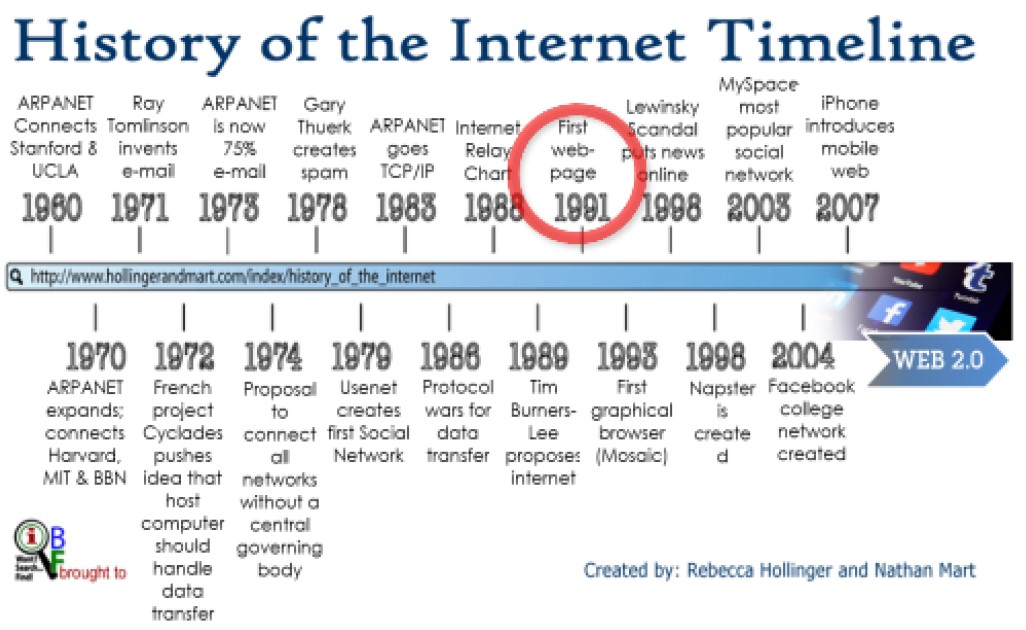
\includegraphics[width=0.9\linewidth]{images/03_lez_fig_01.jpg}
    \caption{History of Internet Timeline}
    \label{fig: Internet Timeline}
\end{figure}

Partiamo dal 1960 e arriviamo al 2007 con il web 2.0. 
Una delle date da ricordare più importanti è il 1991, data nella quale è stata pubblicata la prima web page.

Il nostro spunto di riflessione per questa prima parte della lezione è: quando è nato il moderno Internet? 

\subsection{Chi sono i principali strumenti e i principali attori di Internet?}

In questa seconda parte parleremo proprio di questi strumenti e attori. \par

\begin{itemize}
    \item Il World Wide Web
    \item gli Internet Service Provider
    \item i browser
    \item i motori di ricerca
    \item gli utenti
\end{itemize}

Come avete visto ho indicato gli utenti tra gli strumenti e gli attori del web perché nel web 2.0 gli utenti hanno un ruolo fondamentale di condivisione. Oggi gli utenti non sono più soltanto fruitori di ciò che accade su Internet, ma sono essi stessi artefici di quello che viene pubblicato. E partiamo quindi a cercare di definire chi sono tutti questi soggetti.

\subsubsection{World Wide Web}

Il  World Wide Web è il servizio di Internet che permette di navigare e usufruire di contenuti multimediali collegati tra loro (link) e di altri servizi. Il World Wide Web è il sistema che permette la condivisione di documenti ipertestuali e multimediali. 
Che cosa significa documenti ipertestuali e multimediali? 
Vuol dire che non si tratta soltanto di testo scritto ma che all'interno di questi documenti sono compresi anche immagini, suoni, altre forme di comunicazione e che tutte quante arrivano a costituire un unico documento, continuiamo a chiamarlo così utilizzando un termine tradizionale, ma fruibile in più modi da parte dell'utente.

Per accedere al World Wide Web si utilizza un software particolare detto browser. Quindi il web è un insieme di server web interconnessi.

\subsubsection{Web server}

I web server sono delle applicazioni software in esecuzione su un server che possono gestire le richieste di trasferimento di pagine web a un client. 

Ma i documenti dove sono? 

I documenti sono genericamente detti pagine web e sono memorizzati in porzioni della memoria dei server e sono raggruppati in insiemi più o meno uniformi per aspetto o per contenuti che sono organizzati secondo una qualche struttura. Questi sono detti siti. 
Per essere accessibili le pagine web vengono costruite con dei linguaggi descrittori particolari che permettono di specificare sia il contenuto della pagina, sia il loro formato di visualizzazione sul browser dell'utente.

Da questo punto di vista la visualizzazione è diversa quando l'utente è davanti allo schermo di un computer oppure quando è davanti ad un dispositivo mobile.

Vi sarete resi perfettamente conto ormai che le applicazioni su dispositivo mobile sono sempre più diffuse, che il modo di accedere, il modo di visualizzare i siti è completamente diverso.

La comunicazione tra utente e server così come il trasferimento tra le pagine web sono regolate da dei protocolli di trasferimento così detti e le singole risorse che sono disponibili sulla rete sono individuate univocamente da una serie di caratteri di identificazione universale.

In particolare la URL, \textbf{Uniform Resource Locator}, consente di specificare il nome e la posizione del documento. Poi torneremo su questo punto per comprendere come sia possibile l'identificazione univoca. La caratteristica principale della rete web è che i nodi che la compongono sono tra loro collegati tramite i link, i cosiddetti collegamenti ipertestuali, e in questa maniera formano un enorme ipertesto in modo tale che gli utenti possano navigare e usufruire di contenuti amatoriali e professionali multimediali e non.

La facile reperibilità delle informazioni è resa possibile dalla diffusione, facilità d'uso ed efficienza dei motori di ricerca e dei web browser appunto, in un modello di architettura di rete definito client-server. E quindi torniamo al nostro web server. Un server web, come detto prima, è un'applicazione software che permette di gestire le richieste di trasferimento di informazioni di pagine web di un client. Vediamo in fig. \ref{fig:Tipologie di server web} quali sono i web server più diffusi oggi nel mondo.

\begin{figure}[ht]
    \centering
    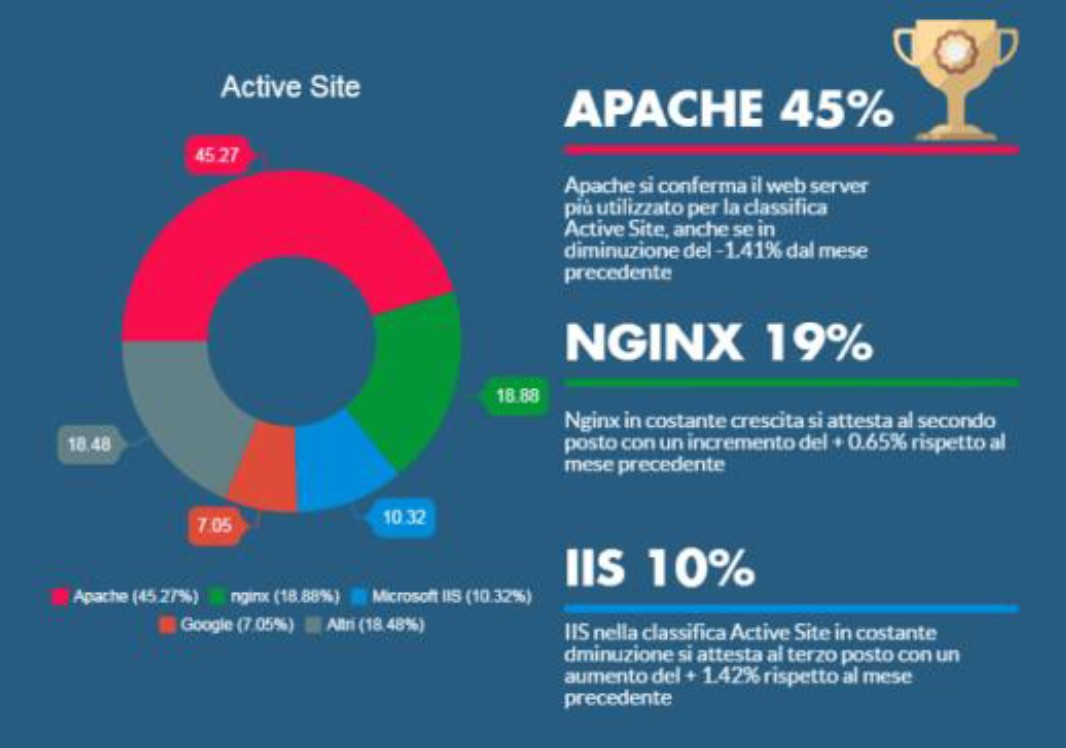
\includegraphics[width=0.8\linewidth]{images/03_lez_fig_02.jpg}
    \caption{Titologie di server web}
    \label{fig:Tipologie di server web}
\end{figure}

I web server più utilizzati nel dicembre 2016 erano principalmente Apache con una diffusione del 45\% seguiti da NGINX al 19\% e poi gli altri, IIS il 18\% e così via. 

Ecco qui un altro schema di riferimento in cui c'è il numero di presenze (fig. \ref{fig:presenza di server web}).
\begin{figure}[ht]
    \centering
    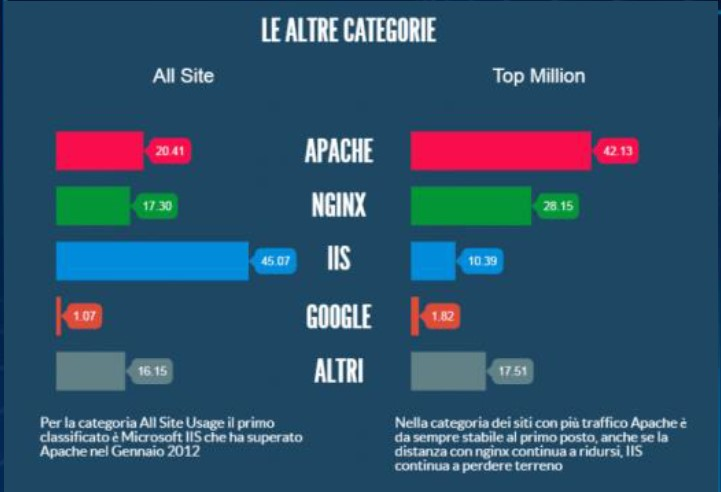
\includegraphics[width=0.8\linewidth]{images/03_lez_fig_03.jpg}
    \caption{Presenza di server web}
    \label{fig:presenza di server web}
\end{figure}

Continuamente nascono dei nuovi server, non sempre riescono ad avere una diffusione tale da aggredire quella che è attualmente la distribuzione.

\subsubsection{ISP Internet Service Provider}

Oltre ai server ci sono gli internet service provider, società che a pagamento permettono l'accesso a internet e forniscono altri servizi come email, spazi per la creazione di siti e così via. Un internet service provider è un fornitore di servizi internet appunto e cioè una struttura a carattere commerciale o un'organizzazione che offre agli utenti, persone fisiche e imprese, l'accesso a internet a pagamento con la stipula di contratti di fornitura. Di solito per la connessione a un internet service provider si utilizza una connessione remota attraverso una linea telefonica, banda larga o attraverso tutte quelle che sono le forme di connessione che la tecnologia riesce a mettere a disposizione degli utenti.

Gli internet service provider permettono o offrono anche dei servizi aggiuntivi fondamentali per la gestione e la fruibilità, cioè la posta elettronica, spazi per la creazione di siti web e quant'altro.

Gli internet service provider non sono tutti uguali fra loro, quelli di primo livello costituiscono la dorsale principale di internet e a questi sono connessi gli internet service provider di secondo livello che fungono da punti di connessione.

Dal 2000 in poi il mercato dell'accesso a internet ha avuto una crescita esponenziale e gli internet service provider hanno aggiunto servizi su servizi e non sono più solo dei punti di accesso, cosa che rimane comunque fondamentale, ma  danno tutta una serie di altre possibilità e in questo modo a seconda delle possibilità che offrono si fanno anche concorrenza fra di loro.

Ogni paese ha i suoi, in Italia l'Associazione Italiana Internet Provider, in UK la ISPA UK, in Francia AFPI e in Europa in generale l'euro ISPA. (fig. \ref{fig:Associazioni_ISP}) \par

\begin{figure}
    \centering
    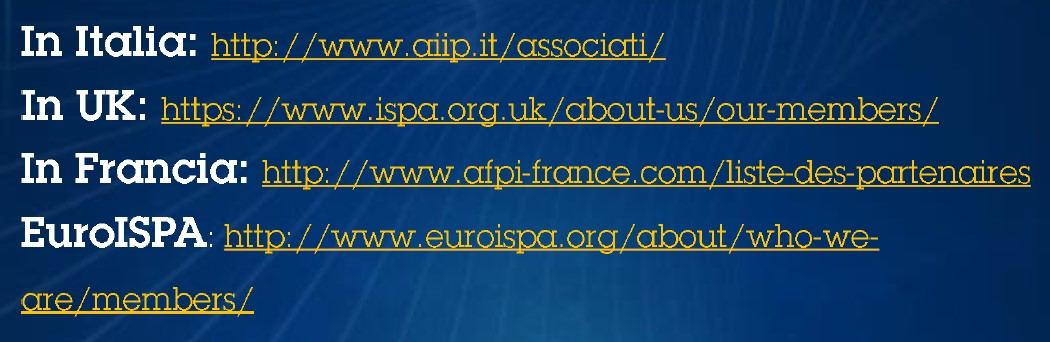
\includegraphics[width=1\linewidth]{images/03_lez_fig_04.jpg}
    \caption{Associazioni ISP}
    \label{fig:Associazioni_ISP}
\end{figure}


\subsubsection{Browser}
I browser sono applicazioni per il recupero, la presentazione, la navigazione di risorse sul web. 
Esempi sono  Google, Firefox, Safari, Microsoft Edge, Opera.

Il browser è fondamentale per poter accedere alla risorse messa a disposizione sul web. Da un lato il programma implementa le funzionalità del client e dall'altro consente la visualizzazione dei risultati, dei contenuti ipertestuali che vengono ricercati.

\subsubsection{Motori di ricerca}
Il motore di ricerca è un sistema automatico che su richiesta analizza un insieme di dati raccolti e restituisce un indice dei contenuti disponibili. I motori di ricerca più utilizzati nel 2017 sono:

\begin{itemize}
    \item Google
    \item Bing
    \item Qwant
    \item Yandex
    \item Ecosia
    \item Duck Duck GO
\end{itemize}

Sono motori di ricerca che hanno delle grandi similitudini fra loro ma anche delle differenze e sono le differenze sulle quali si basa la concorrenza. 

Come ho detto prima, Google assolutamente ha sbaragliato tutti, se consideriamo, il numero di accessi che ha quotidianamente è assolutamente di molto al di sopra di tutti gli altri.

Le caratteristiche di diversificazione sono la velocità, oppure la quantità di notizie di risultati che vengono restituiti, le modalità innovative di presentazione dei risultati stessi.

Avrete forse in passato sentito parlare di una vicenda che ha riguardato le modalità di presentazione dei risultati da parte di Google. Se navigate provate a googlare (è un termine ormai entrato nell'uso comune, non soltanto in Italia ma anche in altri paesi) e provate a cercare Google Spain troverete una serie di risultati relativamente ad una sentenza molto importante della Corte di Giustizia dell'Unione Europea che ha affrontato il tema del trattamento dati personali.

Torneremo su questo argomento in un'altra lezione relativamente al trattamento dati personali da parte dei motori di ricerca e la loro presentazione senza limitazioni di tempo anche a distanza di molti anni. Sulla base di questo si è elaborato un concetto di diritto all'oblio, diritto a essere dimenticati da web, che ha delle caratteristiche diverse rispetto a ciò che è mai stato in precedenza.

Torniamo ai motori di ricerca, i quali:

\begin{itemize}
    \item permettono l'organizzazione dei contenuti e il loro collegamento
    \item stabiliscono una relazione tra la ricerca dell'utente e le informazioni
    \item restituiscono una lista di riferimenti con una breve descrizione di quello che è il contenuto
    \item Attraverso degli hyperlink aprono altri siti o risorse
    \item Per ricordare quali sono state le precedenti ricerche dell'utente installano dei cookies, delle piccole stringhe di testo, che consentono di ricordare quali sono state le ultime ricerche dell'utente e permettono così di velocizzare le attività di ricerca.
\end{itemize}


\begin{figure}[ht]
    \centering
    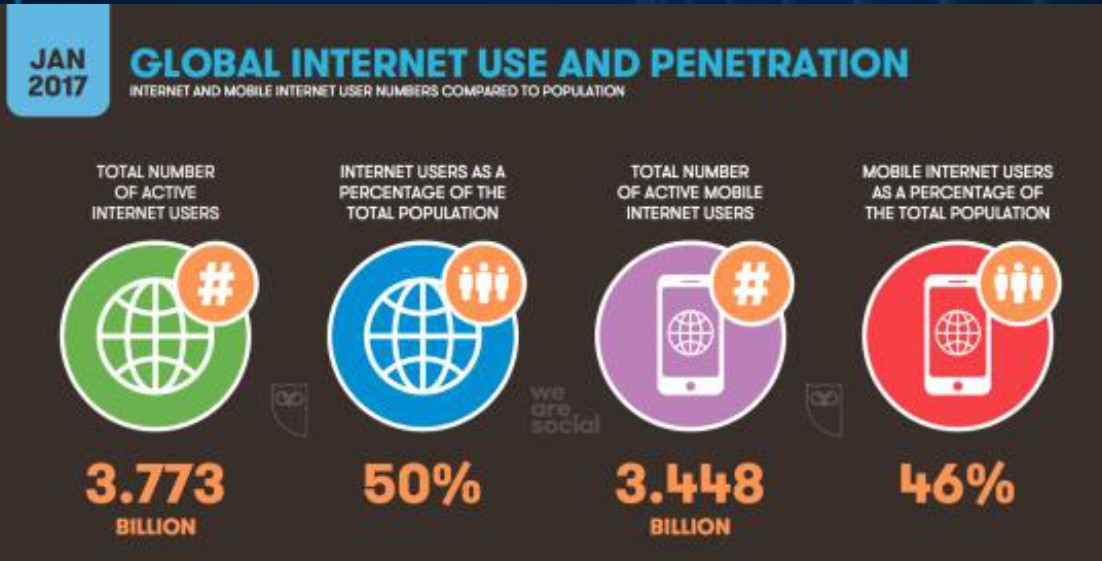
\includegraphics[width=1\linewidth]{images/03_lez_fig_05.jpg}
    \caption{Penetrazione globale di internet}
    \label{fig:penetrazione_globale_internet}
\end{figure}

Nel gennaio 2017 l'uso e la penetrazione globale di internet è descritta in questa slide (fig. \ref{fig:penetrazione_globale_internet}). 

Su 3 miliardi 773 milioni di utenti attivi su internet, il 50\% è la percentuale sulla popolazione globale, il totale dei dispositivi mobili attivi è 3 miliardi e 448 milioni e i dispositivi mobili sono una percentuale del 46\%. 

In quest'altra slide potete vedere la diffusione di internet in base alle regioni del mondo (fig. \ref{fig:diffusione_internet}):
\begin{figure}[ht]
    \centering
    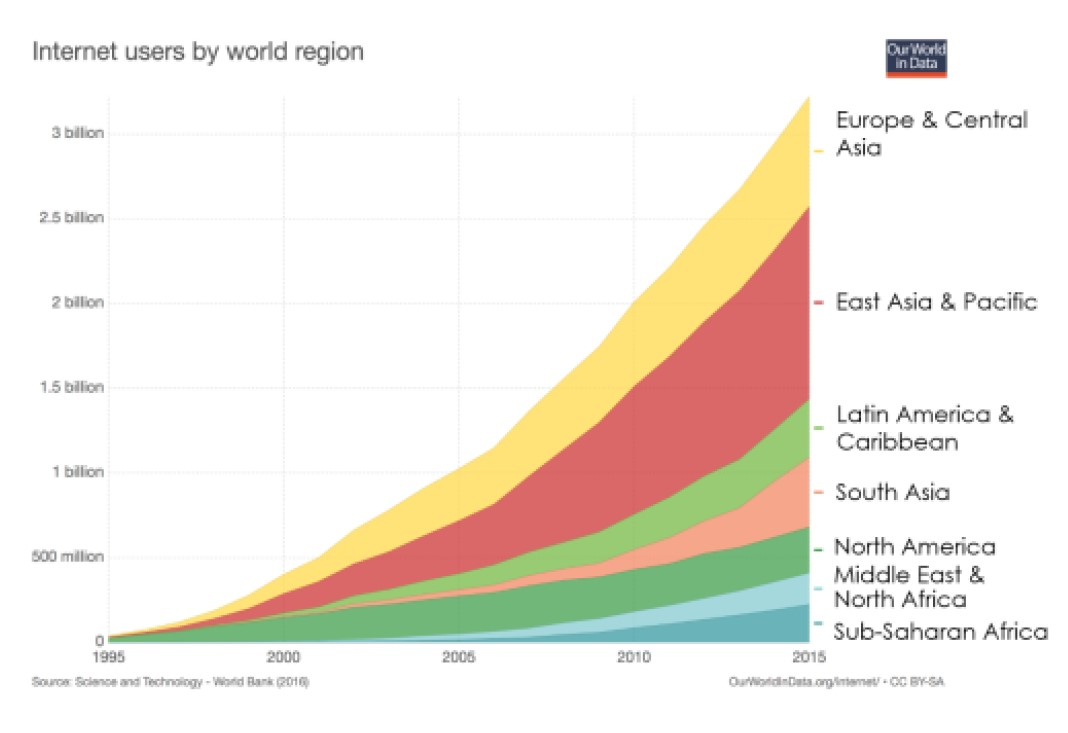
\includegraphics[width=0.9\linewidth]{images/03_lez_fig_06.jpg}
    \caption{Diffuzione di internet negli anni}
    \label{fig:diffusione_internet}
\end{figure}


Europa e Asia centrale, 3 miliardi, Est Asia e Pacifico 2 miliardi circa, America Latina e Caraibi 1 miliardo, Asia del sud, Nord America e così via. Questa è la penetrazione e soprattutto il cambiamento, la curva ascendente che c'è stata tra il 1995 e il 2015. I numeri sono cresciuti in maniera veramente eccezionale. 

Il nostro spunto di riflessione per questa seconda parte della lezione è chi fornisce l'accesso a internet ai cittadini?

\subsection{Identificazione sul web}

Abbiamo accennato all'inizio della nostra lezione che è fondamentale sul web l'accessibilità effettiva alle risorse che ci sono ed è quindi necessario avere una identificazione univoca di ogni utente, di ogni sito e  per questo bisogna rispettare delle regole.

\subsubsection{Gli indirizzi in internet.}

Per accedere ad una risorsa su internet è necessario conoscerne la localizzazione, cosiddetto indirizzo IP.

La URL (Uniform Resource Locator) identifica l'indirizzo sulla rete in modo univoco.

Vedete su questa slide una descrizione di che cos'è la URL (fig. \ref{fig:descrizione_URL}).

\begin{figure}[ht]
    \centering
    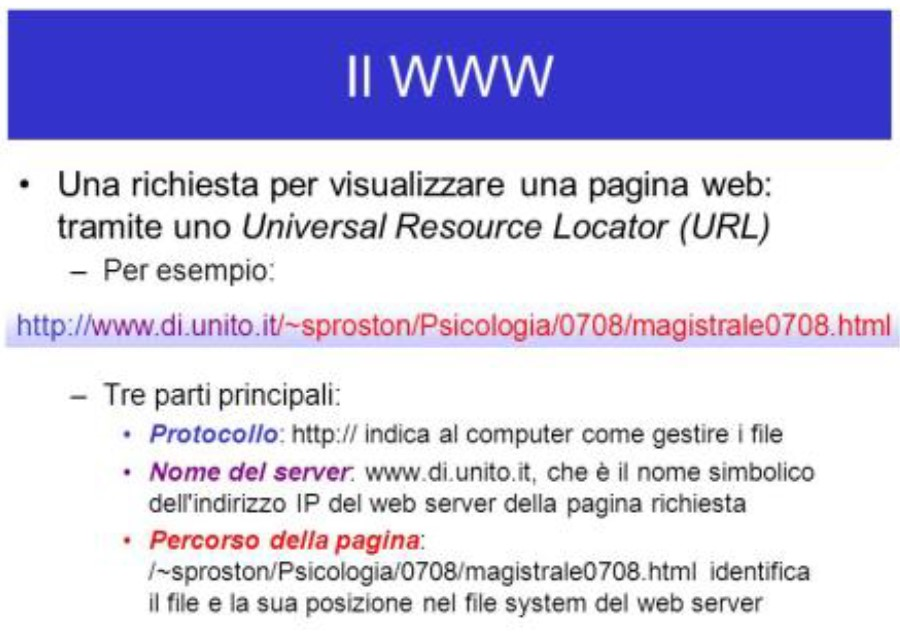
\includegraphics[width=0.9\linewidth]{images/03_lez_fig_07.jpg}
    \caption{Descrizione URL}
    \label{fig:descrizione_URL}
\end{figure}

Ad esempio, http://www.di.unito.it è un indirizzo che è composto di tre parti principali.

Il protocollo http indica al computer come gestire i file, il nome del server www.di.unito.it è il nome simbolico dell'indirizzo IP del web server della pagina richiesta e poi c'è il percorso della pagina.

Tutta questa serie di caratteri alfanumerici identificano il file e la sua posizione nel file system del web server. 
Gli indirizzi in internet sono sempre gli stessi in un certo senso ma un cambiamento importante nel corso del tempo è stata la individuazione dei DNS (domain name server). 
Il DNS consente l'individuazione univoca con un linguaggio alfanumerico comprensibile con un passaggio da codice numerico a una stringa di testo. Grazie ai domain name server per raggiungere i siti si possono utilizzare i nomi a dominio invece degli indirizzi IP, cioè in altri termini ogni sito è raggiungibile attraverso un IP numerico ma ciò che l'utente digita è un nome e questo nome viene riconosciuto come collegato in maniera univoca a quel determinato indirizzo e quindi consente di accedere alla risorsa.

Anche i nomi a dominio così come gli indirizzi IP devono essere univoci, per garantirlo la loro assegnazione è affidata a diversi organismi centrali.

Ma quali nomi a dominio esistono e cosa significano le varie estensioni dei nomi a dominio? I nomi a dominio hanno una struttura gerarchica che adesso vediamo.

\subsubsection{La struttura dei DNS}

\begin{itemize}
    \item Ci sono prima di tutto i top level domain (TLD) o domini di primo livello
          \begin{itemize}
              \item generici gTLD come .org, .net e com. Questi top level domain sono assegnati da una struttura internazionale chiamata ICANN
              \item country code top level domain ccTLD che sono i domini caratteristici dei vari paesi, quindi abbiamo .it, .at, .fr, .uk. Ogni paese ha un dominio caratteristico.
          \end{itemize}
    \item Dopodiché abbiamo i second level domain, i domini di secondo livello
    \item e poi il third level domain (sub domain) che sono definiti nella rete locale.
\end{itemize}

Sia i general gTLD, sia i country code ccTLD sono domini di primo livello. \par

I general Top level domain (gTLD) riguardano:
\begin{itemize}
    \item .com organizzazioni commerciali,
    \item .edu riguardano gli enti di ricerca alle università,
    \item .gov enti governativi,
    \item .int organizzazioni internazionali,
    \item .mil enti militari,
    \item .net enti di gestione della rete,
    \item .org enti diversi di volontariato, associazioni senza scopo di lucro e quant'altro
    \item i domini nazionali, .it, .fr, .uk, .de, ...
    \item .eu le istituzioni europee hanno un dominio EU che è caratteristico
\end{itemize}

\subsubsection{L'assegnazione dei general top level domain (gTLD)}

L'assegnazione dei general top level domain e quindi l'assegnazione degli indirizzi di rete curata dall'\textbf{ICANN, Internet Corporation for Assign Names and Number}, il sito dove andare a verificare, a studiare, esaminare di che cosa si tratta è www.ican.org. 

Parleremo meglio di ICANN in una prossima lezione, ma in questa lezione ci sono alcune indicazioni fondamentali che è bene che voi abbiate.
%-------------------------------------------------------
L'ICANN è stato istituito nel 1998 e incaricato dalle autorità governative degli Stati Uniti. Al giorno d'oggi è invece un ente di gestione internazionale. Potete notare, se fate mente locale a quanto abbiamo detto precedentemente in questa lezione, che l'origine di tutto ciò che riguarda il nostro internet è partita dagli Stati Uniti.

Il coinvolgimento degli altri paesi, in particolare dell'Unione Europea, è avvenuto in un secondo momento e a questo ha corrisposto una effettiva globalizzazione del mondo internet. Ma è per questa ragione che anche gli enti che si occupano della gestione di internet in prima battuta sono nati negli Stati Uniti e in prima battuta sono nati su indicazione degli organismi pubblici statunitensi. Abbiamo parlato dell'Arpanet che partiva dalle autorità militari, ma anche il soggetto che assegna i nomi di dominio, ICANN, è stato in prima battuta incaricato dal governo degli Stati Uniti. Il fatto che oggi sia un ente di gestione internazionale è sicuramente una garanzia di maggiore coinvolgimento anche degli altri Stati.

ICANN (Internet Corporation for Assigned Names and Numbers) ha l'incarico di assegnare gli indirizzi IP ed identificare e gestire i gTLD.

\subsubsection{Assegnazione dei ccTLD}

L'assegnazione dei ccTLD, cioè i Country Code Top Level Domain, è invece curata dai Registrar locali. In Italia la Naming Authority fa capo al CNR (Consiglio Nazionale delle Ricerche), e opera con il Ministero delle Poste e delle Telecomunicazioni (www.nic.it).

L'assegnazione dei Country Code Top Level Domain è in ogni Stato assegnata ad un registrar locale. In ogni Paese quindi c'è un registro locale e in Europa per l'assegnazione dei domini EU c'è l'EURID che è il registrar dei country code top level domain .eu (eurid.eu/en/).

Interessante è il CENTR, l'associazione dei registri dei ccTLD europei che raccoglie tutti quanti i registrar locali. (www.centr.org).

I registrar hanno un contratto/accordo con ICANN, tutti quanti ad eccezione della Germania e della Gran Bretagna. Quindi se andate a fare una verifica sui vari siti dei registrar locali, vedrete che fanno riferimento all'ICANN per mantenere un coordinamento e anche per valutare e verificare quali sono le regole da applicare. La Gran Bretagna e la Germania invece sono completamente autonomi.

\subsubsection{Registrar WHOIS}
I registrar svolgono una funzione molto importante, la funzione WHOIS. 

I registrar mantengono il database in cui sono indicati i dati dei titolari e dei nomi a dominio. Il mantenimento di un database è molto importante, non si tratta soltanto di tenere l'indicazione dei vari indirizzi assegnati, dei nomi di dominio assegnati, ma si tratta di conservare le informazioni relative ai titolari di questi siti e di questi domini. E' possibile un'interrogazione di questi database da parte di chi ha interesse a sapere chi sia il titolare di un nome a dominio, ma i nomi a dominio possono attivare la cosiddetta funzione privacy. 

La funzione privacy è una funzione in base alla quale a fronte di una interrogazione del motore di ricerca si possono avere alcune informazioni legate al titolare della registrazione, ma non tutte. È una funzione che mantiene riservato il nominativo, la denominazione del titolare. Questo ovviamente garantisce il titolare del nome di dominio, ma può mettersi in conflitto con quelle che può essere l' esigenza degli utenti di conoscere chi c'è dietro a un determinato dominio. La questione può interessare quando c'è un trattamento di dati personali, di dati di altri, quando attraverso un determinato sito vengono commessi degli illeciti, quando vengono diffuse delle fake news. L'oscuramento delle informazioni relative al titolare può impedire l'esercizio di altri diritti. 

Ne riparleremo in una prossima lezione, ma intanto il nostro spunto di riflessione per questa terza parte della lezione.

Chi è il responsabile dell'assegnazione di nomi a dominio CCTLD? 

Ora andiamo al riepilogo degli spunti di riflessione.

\begin{itemize}
    \item Quando è nato il moderno Internet?
    \item Chi fornisce l'accesso a Internet ai cittadini?
    \item Chi è il responsabile dell'assegnazione di nomi a dominio ccTLD?

\end{itemize}
La nostra lezione termina qui.
\chapter{Lezione 4 - La Governance di Internet I parte}

In questa lezione inizieremo a parlare di un argomento molto complesso in continua evoluzione, la governance di Internet. Vediamo gli argomenti di oggi:

\begin{itemize}
    \item La governance di Internet
    \item il World Summit on Information Society (WSIS)
\end{itemize}

\section{Governance di Internet}

\subsection{Definizione:}

\textbf{L'Internet Governance è il concetto che include tutte le attività che determinano la direzione dell'uso e dello sviluppo della rete Internet nei suoi vari aspetti, aspetti tecnici, infrastrutturali, aspetti economici e legali, aspetti sociali e politici.}

\subsubsection{Il fondamento della internet governance:}

\textbf{Il principio fondamentale della internet governance è che nessun soggetto può gestire autonomamente Internet, cioè la rete deve restare globalmente distribuita e priva di un organo di controllo centrale.} 

Questa necessità di un controllo diffuso e la volontà di evitare che ci sia un controllo centralizzato è da un lato necessaria per la struttura della rete e per l'immensità (La rete coinvolge e riguarda attori in tutto il mondo e quindi sarebbe estremamente complesso prenderne il controllo) dall'altro il punto è che si vuole mantenere la rete come strumento di libertà e di possibilità di circolazione libera delle informazioni e di sviluppo per tutta la società.

\subsubsection{Le componenti della internet governance}

La internet governance si articola su tre livelli:

\begin{itemize}
    \item Un livello fisico costituito dall'infrastruttura. Le infrastrutture della rete sono fondamentali per il passaggio delle informazioni.
    \item Un livello logico, il codice con il quale si scrivono le informazioni che poi diventano fruibili per la collettività.
    \item i contenuti, le informazioni che sono immesse non soltanto dai professionisti ma anche dagli utenti e che sono quelle che circolano ovunque, che sono intelligibili ovunque.
\end{itemize}

I protagonisti:

\begin{itemize}
    \item Gli stakeholders della rete sono innanzitutto i governi,
    \item le istituzioni nazionali e internazionali,
    \item le imprese private,
    \item la società civile.
\end{itemize}

Come potete vedere c'è una situazione multilivello. La partecipazione possibile sulla rete è una partecipazione veramente di tutti gli attori, di tutti i diversi livelli di soggetti che interagiscono in modo diverso e che possono contribuire allo sviluppo della società dell'informazione in modo diverso.

Attività e obiettivi:

\begin{itemize}
    \item la condivisione
    \item le regole
\end{itemize}

Le regole in particolare si concretizzano nello sviluppo e nell'applicazione di principi e di procedure decisionali e programmi condivisi.

La necessità di condivisione è sentita a tutti i livelli però dall'altra parte si pone la necessità di regole che permettano da un lato di consentire a tutti di usufruire allo stesso modo delle risorse e usufruirne sia come fruitori finali ma anche come artefici e come attori di quanto viene distribuito e sia per cercare di evitare abusi della rete che sono comunque sempre possibili.

Le scelte che riguardano la governance di internet hanno delle ricadute importanti sui governi a livello politico e sulla società tutta anche a livello economico. Sono diverse le iniziative che sono state assunte nel corso degli ultimi 20 anni quindi a partire dai primi anni 2000 soprattutto per gestire la governance di internet, per individuare il modo migliore di creare una governance su internet. Le iniziative che sono state assunte sono iniziative assunte soprattutto a livello internazionale proprio in considerazione del fatto che la rete è qualcosa di globale. Attualmente tra i temi importanti che sono affrontati nell'ambito della internet governance ci sono:
 
\begin{itemize}
    \item la cyber security
    \item il cyberbullismo
    \item la lotta all'illegalità intesa ad ampio spettro
    \item i temi legati alla violazione del copyright
\end{itemize}

La internet governance quindi è qualcosa che coinvolge la collettività tutta a livello internazionale e che appunto deve essere affrontata con degli strumenti di carattere internazionale.

Bisogna distinguere tra la internet governance e la e-governance.\par

La i-governance non  va  confusa con la e-governance che indica le iniziative di un governo nazionale per la fornitura di servizi via internet a cittadini, imprese e altri governi ed è legata allo sviluppo delle infrastrutture informatiche e di telecomunicazione.

A questo punto un nostro primo spunto di riflessione. Qual è il principio fondamentale della internet governance?

\section{World Summit on Information Society}
Il World Summit on Information Society, il vertice internazionale della società dell'informazione, è stato lanciato con la risoluzione 56/183 dell'Assemblea Generale delle Nazioni Unite il 21 dicembre 2001. In questa occasione l'Assemblea Generale ha approvato lo svolgimento del vertice mondiale della società dell'informazione, WSIS, iniziando e avviando due fasi. La prima fase si è svolta a Ginevra dal 10 al 20 di dicembre 2003, la seconda fase si è svolta a Tunisi dal 16 al 18 novembre 2005.

Quindi, la risoluzione 56/183 dell'Assemblea Generale delle Nazioni Unite è il punto di partenza del World Summit on Information Society e ha come presupposto il fatto che il cambiamento tecnologico trasforma l'ambiente in cui si è sviluppata la società dell'informazione.

Quali azioni si intendevano portare avanti? Innanzitutto, ci si è resi conto che il World Summit doveva essere una piattaforma in evoluzione continua, perché è la stessa società dell'informazione in evoluzione continua proprio in considerazione dell'evoluzione e dello sviluppo della tecnologia. E quindi la promozione di qualunque tipo di policy, qualunque tipo di attività in questo ambito deve coinvolgere i livelli nazionali, regionali e interregionali, ma deve avere un luogo, un punto di riferimento in cui effettivamente sia possibile scambiarsi delle idee e in cui sia possibile costruire qualcosa di nuovo.

La struttura iniziale data al World Summit dell'Information Society quella del 2003-2005, aveva l'obiettivo di tener conto dell'evoluzione per individuare i successivi sviluppi.

Anche successivamente, dopo il 2005, il World Summit si è continuato a tenere periodicamente e ha portato delle grandi e importanti novità.

Vediamo la prima fase:

\subsection{nel 2003, dichiarazione di Ginevra}

L'obiettivo individuato nell'ambito del World Summit di Ginevra era l'individuazione di una volontà politica di stabilire le basi per una società dell'informazione per tutti. Società dell'informazione per tutti vedremo che comporta una serie di iniziative. Tutti a qualunque età, e quindi un tema di digital divide legato alle generazioni. Tutti vuol dire tutti i luoghi e tutti i paesi del mondo e quindi questo significa portare l'infrastruttura tecnologica che consente di partecipare al mondo internet anche nei luoghi più sperduti del mondo. Tutti vuol dire questioni economiche, quindi evitare di avere un divario tra coloro che hanno possibilità economiche di interagire con determinati strumenti tecnologici e coloro che non ce le hanno. Tutti vuol dire formazione e informazione sufficiente per comprendere quali sono i temi fondamentali nella società dell'informazione.

Il \textbf{piano d'azione per lo sviluppo sostenibile} è stato elaborato all'interno della dichiarazione di Ginevra. \par

I protagonisti individuati dal summit di Ginevra:
%----------------------------------------------------------------------
\begin{itemize}
    \item i governi. I governi hanno un ruolo guida e un ruolo di sviluppo nell'attuazione delle strategie della società dell'informazione nazionali e globali, strategie che devono essere lungimiranti e sostenibili da tutti i punti di vista e tali da permettere di creare e portare avanti un ambiente favorevole e competitivo per gli investimenti necessari all'infrastruttura della società dell'informazione e per lo sviluppo di nuovi servizi.
    
    \item Il settore privato e la società civile in un dialogo con i governi possono svolgere un ruolo consultivo importante nell'elaborazione delle strategie elettroniche nazionali.
    
    \item La società civile è direttamente impegnata in quello che è il mondo della società dell'informazione e della comunicazione. Soltanto la partecipazione di tutti gli attori della società civile, siano essi persone individui, persone fisiche, siano essi soggetti che rappresentano interessi che vengono dalla società civile è essenziale per dare delle indicazioni su quello che è lo sviluppo sostenibile, lo sviluppo utile della società dell'informazione.
    
    \item le istituzioni internazionali e regionali.
\end{itemize}

L'impegno del settore privato accanto a quello dei governi è importantissimo per l'evoluzione della società dell'informazione, delle tecnologie, dell'informazione e della comunicazione, sia per la realizzazione delle infrastrutture, sia per la creazione di informazioni e l'immissione di contenuti e la gestione anche dei contenuti, e sia per lo sviluppo delle applicazioni che consentono di offrire servizi al grande pubblico. Il settore privato quindi non è soltanto un attore del mercato ma svolge un ruolo in un contesto di sviluppo sostenibile il più ampio possibile.

Le istituzioni pubbliche internazionali e regionali, quando si parla di istituzioni regionali non si intende ovviamente alle regioni di un singolo paese ma a macro regioni, soggetti che comprendono diversi paesi nelle diverse aree geografiche.

Le istituzioni internazionali hanno il ruolo determinante perché in un contesto nel quale il collegamento è un collegamento ampio all'interno del mondo, all'interno di una società globale, non è pensabile che il ruolo di gestione, organizzazione, sviluppo e quant'altro sia limitato ad un ambito di carattere nazionale.

Le tematiche sono complessive, sono globali. La rete ha come particolarità proprio il fatto di essere accessibile e fruibile in tutto il mondo, senza limitazioni e confini di carattere geografico e questa è la ragione per la quale qualunque tipo di valutazione, qualunque tipo di gestione deve essere condiviso a tutti i livelli.

Oltre ad individuare gli stakeholders cioè i componenti del mondo della società dell'informazione, la dichiarazione di Ginevra si è posta anche degli obiettivi. \par

\subsubsection{2003 - Obiettivi}

\textbf{L' obiettivo primario è la costruzione di una società dell'informazione inclusiva nella quale le tecnologie dell'informazione e della comunicazione sono al servizio dello sviluppo.}

L'obiettivo di carattere generale è quello di promuovere il più possibile l'inclusione a tutti i livelli.

\begin{itemize}
    \item comunità cioè trovare il modo di collegare tutti i luoghi del mondo, anche i più piccoli villaggi, alla rete per includerli nello scambio di informazioni, stabilire quindi dei punti di accesso per tutte le comunità.
    
    \item Istruzione e ricerca: poter collegare università, college e scuole consente di condividere le informazioni e la cultura a tutti i livelli.
    
    \item gli uffici pubblici, il tema delle attività della e-democracy, quindi delle attività che collegano le amministrazioni pubbliche ai cittadini, rendere accessibile tutto ciò che è la vita pubblica di un cittadino all'interno del proprio paese.
    
    \item accessibilità vuol dire adattare i programmi e gli strumenti alla portata di tutti e quindi ancora una volta dai bambini agli anziani senza che vi siano limitazioni legate al livello diverso di preparazione culturale.
    
    \item i contenuti, occorre incoraggiare lo sviluppo di contenuti e mettere in atto le condizioni tecniche per facilitare la presenza e l'uso di tutte le lingue del mondo su internet, quindi non soltanto le lingue più diffuse ma veramente tener conto della ricchezza linguistica dei paesi del mondo e consentire a tutti un accesso. Questo significa ad esempio implementare degli strumenti di traduzione dei contenuti, implementare l'utilizzo anche di scritture e caratteri che non sono comunemente utilizzati e anche questo è uno strumento per far sì che tutti nell'ambito del mondo abbiano accesso alle tecnologie dell'informazione e della comunicazione.
\end{itemize}

Per raggiungere questi obiettivi occorre lavorare sulla formazione e sull'informazione a partire dai livelli scolastici dei più piccoli, quindi a partire dai primi passi dei bambini e per andare avanti fino al livello universitario e poi ancora continuare a mantenere il collegamento fra le biblioteche, fra i musei, fra tutte quelle istituzioni che diffondono e raccolgono la cultura.
Occorre far sì che tutta la popolazione abbia la possibilità di accedere a servizi della società dell'informazione dai più piccoli villaggi ma anche in tutti gli ambiti sociali e culturali dei paesi.

\subsubsection{2003 - Linee di azione}

\begin{itemize}
    \item  infrastrutture, per infrastrutture si intende la banda larga, si intende il satellite e tutte le infrastrutture che consentono la trasmissione dei dati. L'infrastruttura come detto più volte è essenziale per raggiungere l'obiettivo dell'inclusione digitale consentendo a tutti un accesso universale, sostenibile, ubiquo e accessibile, tenuto conto di quelle che sono le soluzioni via via sviluppate nei diversi paesi e che possono richiedere delle fasi di transizione.
    
    \item accesso all'informazione e alla conoscenza con tutti gli strumenti possibili
    
    \item sviluppo delle competenze, ognuno dovrebbe poter avere le competenze necessarie per beneficiare pienamente della società dell'informazione, pertanto la creazione di capacità e l'alfabetizzazione informatica sono essenziali. Le tecnologie dell'informazione e della comunicazione possono contribuire a raggiungere un'istruzione universale, ad ottenere e ad implementare l'istruzione universale in tutto il mondo, occorre creare gli strumenti per erogare formazione anche agli insegnanti i quali a loro volta potranno poi aiutare i propri allievi a raggiungere determinati obiettivi di competenza. Occorre creare strumenti di formazione permanente e comprendere, all'interno di questi strumenti, anche persone che hanno maggiore difficoltà ad accedere agli strumenti di formazione e di informazione migliorandole anche le competenze professionali.
    
    \item fiducia e sicurezza, per poter stare su Internet occorre avere fiducia nell'uso delle tecnologie, delle informazioni e della comunicazione e quindi occorre promuovere la cooperazione tra i governi anche per proteggere l'integrità dei dati, per proteggere l'integrità della rete, per contrastare e prevenire la diffusione di comportamenti criminali. Quindi nell'obiettivo fiducia e sicurezza c'è la prevenzione del cybercrime, la prevenzione della sicurezza delle informazioni e la tutela della privacy, della riservatezza nella rete.
    
    \item ambiente sicuro, occorre sviluppare tecnologie e strumenti che consentano di mantenere la sicurezza nell'ambito della rete.
    
    \item applicazione delle ICT in diversi settori, lo sviluppo sostenibile della tecnologia, dell'informazione e della comunicazione deve riguardare tutti i settori, dalla pubblica amministrazione alle imprese, dall'istruzione alla formazione, dalla sanità all'occupazione, all'ambiente, all'agricoltura e alla scienza.
    
    \item questo obiettivo di tener conto dell'applicazione della tecnologia nell'ambito dell'applicazione della tecnologia in tutti i settori consente ancora una volta di avere la massima inclusione.
    
    \item sviluppo dell'identità e della diversità culturale e linguistica attraverso l'uso delle lingue che consente di includere la cultura e quindi di tener conto e di sviluppare l'identità culturale, tener conto delle tradizioni, tener conto delle religioni senza escludere nessuno in un concetto di massima inclusione.
    
    \item i media hanno un ruolo fondamentale in questo contesto per la creazione di contenuti corretti, per la ricerca e la diffusione di un'informazione corretta.
    
    \item Dimensione etica, l'etica nella società dell'informazione dovrebbe essere soggetta a valori universalmente condivisi. Trovare valori universalmente condivisi non è semplice data la diversità presente nel mondo.
    
    \item cooperazione internazionale e regionale come detto è fondamentale il collegamento e la cooperazione fra soggetti nell'ambito del mondo intero per riuscire a trovare dei punti di riferimento comuni.
\end{itemize}

L'agenda di Ginevra del 2003 dava uno spunto, un ponte verso il futuro.

\subsection{2005 - agenda di Tunisi}

Nel 2005 l'agenda di Tunisi ribadisce che l'attuazione del World Summit Information Society deve tener conto delle linee di azione stabilite a Ginevra. Nell'agenda di Tunisi si è ribadito e si è chiarito il ruolo delle agenzie e delle Nazioni Unite in questo sviluppo. 

Con l'agenda di Tunisi ci si è resi conto della necessità di avere e creare nuove risorse finanziarie per stare al passo con l'evoluzione della tecnologia e ci si è resi conto e si è sottolineata l'importanza della sostenibilità per le piccole e medie imprese. Non solo le grandi compagnie ma anche le piccole e medie imprese devono poter essere incluse a tutti i livelli all'interno dello sviluppo della società dell'informazione.

Ci si è resi conto, inoltre, della sempre più crescente importanza all'interno di questo contesto dell'apporto della società civile, delle persone, dei cittadini, a fianco ai grandi stakeholders quali governi e le imprese di grandi dimensioni.

Nello sviluppo delle tematiche le organizzazioni internazionali, le agenzie delle Nazioni Unite possono svolgere un ruolo fondamentale perché hanno degli osservatori privilegiati rispetto a quelle che sono le grandi tematiche che coinvolgono il mondo intero. E quindi nella definizione della internet governance si è ribadita la necessità di avere un punto di riferimento comune per tutti e per questa ragione si è deciso di affrontare le nuove sfide con dei punti di riferimento più precisi.

\subsubsection{2005 - Internet governance}

\begin{itemize}
    \item Nell'internet governance, così come indicato nel summit di Tunisi del 2005, si tiene conto dei nomi a dominio, dei numeri di protocollo e degli indirizzi IP come strumenti di contatto e collegamento con individuazione univoca. Parleremo in una delle prossime lezioni del significato dei nomi a dominio, dei numeri di protocollo e degli indirizzi IP e di qual è il loro ruolo nella società dell'informazione e della comunicazione.

    \item è necessario coinvolgere in misura sempre maggiore i diversi stakeholders,
    
    \item è necessario coinvolgere i paesi in via di sviluppo,
    
    \item è necessario individuare delle priorità.
    
    \item nelle priorità individuate nel 2005 c'era il multilinguismo, i contenuti locali, lo spam e la cybersecurity. Inoltre si ribadì l'importanza dell'individuazione di tecnologie standard comuni perché l'utilizzo di diversi tipi di tecnologie poteva creare un digital divide fra diversi paesi in base alla scelta di una tecnologia piuttosto che un'altra.
    
    \item come luogo per esprimere le varie potenzialità e le varie idee è stato istituito l'\textbf{Internet Governance Forum, IGF}, di cui parleremo nella prossima lezione
\end{itemize}

Negli anni successivi al 2005, ogni anno si è tenuto un summit dell'informazione e della comunicazione ma arriviamo al summit al 2015.

\subsection{2015 - ICT e sviluppo sostenibile}

In questo summit abbiamo l'individuazione, la creazione e l'avvio dell'Agenda per sviluppo Sostenibile attuata con la risoluzione dell'Assemblea generale delle Nazioni Unite 70/1 e si è varata l'Agenda 2030 per lo Sviluppo Sostenibile. 

L'Agenda 2030 riconosce e promuove il ruolo delle tecnologie, delle informazioni e della comunicazione (ICT).

L'agenda 2030 per lo Sviluppo Sostenibile riguarda diverse aree dello sviluppo della collettività, le Nazioni Unite hanno ribadito ancora una volta l'importanza delle tecnologie dell'informazione e della comunicazione per lo sviluppo generale di tutti gli ambiti e di tutti i contesti. Quindi non parliamo soltanto di tecnologie per l'informazione ma parliamo di tecnologie per qualunque ambito di interesse del mondo. E quindi anche l'Agenda 2030 ribadisce la necessità di includere in maniera complessiva nell'educazione e nella promozione dell'apprendimento tutte le fasce sociali, tutti i paesi del mondo e tutte le età.

L'Agenda 2030 per lo Sostenibile tra i suoi obiettivi riconosce la necessità di promuovere l'uguaglianza a vario livello e in particolare di coinvolgere il genere femminile, all'epoca ancora non adeguatamente rappresentato e non adeguatamente presente nel mondo della tecnologia.

Ancora per lo sviluppo sostenibile si sottolinea l'importanza dell'evoluzione e della possibilità di accesso alla tecnologia attraverso lo sviluppo di strumenti nuovi. Si riconosce l'importanza di sviluppare delle tecnologie abilitanti che consentano di accedere fin dall'inizio alle informazioni e alla rete. 

Sempre nel 2015 il World Summit Information Society indica le nuove sfide tenendo in considerazione l'Agenda per il 2030.

\subsection{2015 - WSIS verso nuove sfide}

\begin{itemize}
    \item L'uomo è al centro.  Il World Summit riafferma l'impegno per costruire una società dell'informazione e della comunicazione incentrata sulle persone che sia inclusiva e orientata allo sviluppo in cui tutti possano creare contenuti, accedere, utilizzare e condividere informazioni e conoscenze, consentendo agli individui, alle comunità e ai popoli di raggiungere il loro pieno potenziale di sviluppo e migliorare la qualità della propria vita.
    
    \item ICT e sviluppo sostenibile. Il potenziale delle tecnologie dell'informazione e della comunicazione può essere sfruttato come già indicato dall'Agenda per lo sviluppo sostenibile 2030 per raggiungere proprio quegli obiettivi. E quindi sono invitati tutti i governi, la società civile, il settore privato a lasciarsi coinvolgere e a collaborare nella promozione della società dell'informazione.
    
    \item individua alcuni temi nuovi, nuovi rischi sociali e per la salute. L'incremento dell'utilizzo delle tecnologie ha degli aspetti positivissimi come si è visto ma comincia a manifestare anche delle problematiche di cui occorre tener conto e che occorre affrontare nei successivi sviluppi. Da un lato un tema sociale, l'utilizzo delle tecnologie e dell'informazione come strumento oramai quasi principale di gestione delle relazioni, comincia a evidenziare alcuni problemi rispetto ai quali occorre porsi degli interrogativi e che occorre iniziare ad affrontare. Ad esempio, ne parleremo in una delle nostre prossime elezioni, il tema del linguaggio come strumento non di inclusione ma di esclusione, la discriminazione o l'odio espressi attraverso un linguaggio all'interno di un ambiente sociale del quale fa parte una larghissima parte della comunità. Allo stesso tempo cominciano a manifestarsi dei fenomeni nuovi che possono avere un impatto alla salute legati ad esempio ad una dipendenza eccessiva dalle tecnologie. Sono elementi di cui occorre tener conto per vedere non soltanto gli aspetti positivi della tecnologia ma anche vederne gli aspetti negativi, affrontarli e trovare delle soluzioni. Questo tema verrà sviluppato negli anni successivi al 2015.
    
    \item Altro tema che comincia a diventare importante di cui occorre tenere conto è il finanziamento. Lo sviluppo delle tecnologie dell'informazione e della comunicazione richiede di mettere in campo delle risorse economiche estremamente ingenti. Risorse economiche che possono essere reperite all'interno del settore privato in quanto a volte è più difficile reperirle all'interno del settore pubblico, all'interno dei governi con quello che può conseguirne in termini anche di controllo. Il potere economico nella gestione della società dell'informazione consente il controllo. D'altra parte lo sviluppo della tecnologia richiede ingenti finanziamenti. Occorre quindi trovare delle modalità corrette, delle modalità sostenibili per continuare a sviluppare le tecnologie nella maniera migliore e più aperta. Occorre trovare delle forme di investimento che mantengano la libertà nello sviluppo e nell'attività di ricerca.
    
    \item libertà di espressione privacy. Nella società dell'informazione e della telecomunicazione è strumento di diffusione della conoscenza, è strumento attraverso il quale è possibile informarsi, è strumento attraverso il quale è possibile informare. A fronte di questo bisogna tener conto e occorre trovare degli strumenti per ottemperare questo aspetto, il diritto all'informazione, con i diritti della persona e in particolare il diritto alla propria riservatezza, alla propria privacy, al controllo delle informazioni che girano sulla rete e che vengono diffuse. Di questo come vedremo si sono occupate le istituzioni internazionali e in particolare l'Unione Europea con provvedimenti che sono stati assunti successivamente al 2015 e di cui parleremo in una delle prossime lezioni.
    
    \item la sicurezza delle informazioni. In un mondo, in un contesto nel quale le informazioni sono per così dire il pane quotidiano, nel quale le informazioni diventano un bene primario, nel quale le informazioni sono anche merci di scambio, occorre individuare, sviluppare tutto ciò che riguarda la sicurezza delle informazioni stesse e quando si parla di sicurezza si intendono diversi aspetti.
    
    \item  Sicurezza delle informazioni vuol dire evitare che le informazioni possano essere rubate, possono essere acquisite illecitamente. Sicurezza delle informazioni vuol dire evitare che le informazioni possano essere compromesse e non corrispondere più al vero. Sicurezza delle informazioni vuol dire mantenere la riservatezza quando si tratta di informazioni che non possono essere condivise con tutti. Mantenere e sviluppare la sicurezza delle informazioni vuol dire anche incrementare la fiducia delle persone rispetto all'uso delle proprie informazioni sulla rete. E quindi questo tema è in continuo sviluppo e deve essere oggetto di ricerca e promozione.
\end{itemize}


Arrivati a questo punto alcune sono le domande a cui potete rispondere. Gli spunti di riflessione.
\begin{itemize}
    \item Quali sono gli stakeholders coinvolti nella internet governance?
    \item Quali sono le sfide indicate dal World Summit for the Information Society per il futuro della società dell'informazione?
    \item Qual è il principio fondamentale della internet governance?
    \item
\end{itemize}

\chapter{Lezione 5 - La Governance di Internet II parte}

Gli argomenti di oggi:

\begin{itemize}
    \item Internet Governance Forum
    \item il ruolo dell'Europa
\end{itemize}

\section{Internet Governance Forum IGF}

L'Internet Governance Forum è stato promosso dalle Nazioni Unite nel World Summit for Information Society che si è tenuto a Tunisi nel novembre del 2005. Il forum è stato convocato per la prima volta nei mesi di ottobre e novembre del 2006 e successivamente ogni anno si sono svolti degli incontri di questo forum nel quale si sono incontrati e scambiati opinioni tutti gli stakeholders che sono interessati alla governance di Internet. Ricorderete che tra gli stakeholders per la governance di Internet vi sono i governi, le imprese private e la società civile. Si parla quindi di un contesto nel quale si cerca di rappresentare, di ascoltare la voce di tutti coloro che ad ogni titolo sono parte del mondo Internet e quindi appunto sono interessati alla sua governance.

Cosa si tratta nell'Internet Governance Forum?

Si affrontano tutte le tematiche che possono interessare la governance di Internet e dobbiamo sempre ricordare che in questo contesto vi sono degli aspetti di carattere politico, vi sono degli aspetti di carattere tecnico e vi sono le questioni complesse legate anche al rapporto politico fra i diversi Stati e fra i diversi attori. L'Internet Governance Forum non ha dei poteri decisionali ma è un luogo, una struttura, un'organizzazione che nonostante non abbia poteri decisionali è diventata un punto centrale di riferimento per tutti i dibattiti che riguardano il mondo Internet.

Internet Governance Forum che cosa è?

\begin{itemize}
    \item Un luogo di incontro multilaterale aperto a tutti
    \item nel quale discutere della governance di Internet
    \item e affrontare regole, procedure, infrastrutture e programmi che ne determinano il funzionamento e l'evoluzione
\end{itemize}

L'elemento fondamentale che caratterizza l'Internet Governance Forum è la partecipazione di tutti, una multiparticipazione nella quale l'espressione delle valutazioni e delle idee risente della provenienza dei diversi Stackholders e la partecipazione è caratterizzata dalla democrazia e dalla trasparenza. \par

Mandato e temi dell'Internet Governance Forum:

\begin{itemize}
    \item L'obiettivo è facilitare la discussione e il dialogo tra diversi organismi sui temi della governance di Internet.
\end{itemize}

Il mandato dell'Internet Governance Forum è quello di discutere delle questioni di politica pubblica relative agli elementi chiave per la governance di Internet e promuovere la sostenibilità, la solidità, la sicurezza e la stabilità e lo sviluppo di Internet.

Non è semplice il dialogo tra i diversi attori ed è per questo che l'Internet Governance Forum deve trovare il modo di facilitarlo e deve aiutare e facilitare lo scambio di buone pratiche coinvolgendo per quanto possibile le competenze accademiche, scientifiche e tecniche dei diversi paesi che partecipano. Attraverso queste attività nel corso degli anni si sono raggiunti dei risultati interessanti.

Quali i temi principali?

\begin{itemize}
    \item sostenibilità
    \item sicurezza
    \item stabilità e sviluppo
\end{itemize}

Come funziona l'Internet Governance Forum?

Abbiamo visto che la sua istituzione è partita direttamente dall'Assemblea Generale delle Nazioni Unite attraverso il World Summit for Information Society.

Come è stato strutturato l'Internet Governance Forum? Il funzionamento prevede una partecipazione multilaterale attraverso degli incontri virtuali, gruppi di discussione tematici e riunioni periodiche. 

Il codice di condotta dell'Internet Forum prevede delle regole semplici:

\begin{itemize}
    \item rispetto e non discriminazione
    \item focus su temi specifici
    \item partecipazione informata di tutti gli attori
    \item trasparenza
    \item etica e integrità
\end{itemize}

Il forum ha una sua localizzazione presso l'Assemblea Generale delle Nazioni Unite a Ginevra ed è sostanzialmente un segretariato del quale fanno parte un gruppo di persone che si occupano delle attività pratiche. Il forum è affiancato da un gruppo di lavoro, il Multi-Stakeholder Advisory Group (MAG) che è composto di 50 membri nominati dal Segretario Generale delle Nazioni Unite individuati dai governi, dal settore privato, dalla società civile e dalla comunità tecnica. Il Multi-Stakeholder Advisory Group è stato costituito sempre nel 2006 e supporta il forum nella organizzazione e nella programmazione delle attività annuali.

I componenti del MAG collaborano con il forum per:
\begin{itemize}
    \item individuazione dei temi di discussione
    \item pianificazione degli incontri
    \item selezionare le relazioni
\end{itemize}

\subsection{Gli Internet Governance Forum locali}

L'Internet Governance Forum è il punto di riferimento centrale, è la struttura, chiamiamola così, centrale, ma a fianco ad essi sono nati nel corso degli anni una serie di strutture diversificate a livello locale, inteso come a livello nazionale ma anche a livello di macroaree, macroregioni o anche per aree tematiche. Gli Internet Governance Forum locali sono collocati in diversi paesi del mondo:

\begin{itemize}
    \item per l'Italia  (https://www.isoc.it/igfitalia)
    \item Forum regionali (Europa, Africa, Asia, eccetera)
    \item Forum di area di interesse (Forum dei Giovani)
\end{itemize}

L'individuazione delle aree di riferimento degli Internet Governance Forum è basata su dei criteri di carattere geografico, aree geografiche, criteri di carattere culturale e criteri linguistici. Tutti gli Internet Governance Forum locali aderiscono a Internet Governance Forum e partecipano alle conferenze annuali dell'Internet Governance e portano avanti anche delle conferenze a livello locale e regionale. L'obiettivo di questa struttura così organizzata è quello di consentire e agevolare la massima partecipazione possibile a questo Forum che come detto è un Forum che deve essere multipartecipato e quindi poter ascoltare le esigenze che provengono da tutti i livelli di coloro che accedono e partecipano ad Internet.

Per quanto riguarda l'Internet Governance Forum italiano, è coordinato dalla Internet Society Italia in collaborazione con il CNR, il Consiglio Nazionale delle Ricerche, ed è iniziato e partito nel 2008, quindi ha ormai 10 anni di storia, ed è partito con la partecipazione dei rappresentanti del governo, del settore privato e della società civile.

Spunti di riflessione. Quali obiettivi ha Internet Governance Forum? \par
Passiamo adesso alla seconda parte della nostra lezione.

\section{Il ruolo dell'Europa}
L'Unione Europea contribuisce da oltre 15 anni al sostegno e allo sviluppo di Internet e ha svolto e continua a svolgere una funzione essenziale nella vita di tutti. L'Unione Europea non può restare al di fuori di quella che è la governance di Internet e quindi ha operato in maniera organizzata e strutturata in modo da portare le istanze dei paesi europei e dare le proprie indicazioni, le proprie direttive.

Obiettivo ancora una volta è la promozione dell'innovazione e della crescita, la promozione del commercio e della democrazia e dei diritti umani. Nel 2014 in particolare l'Unione Europea ha preso una posizione importante con una comunicazione dedicata al proprio ruolo nella governance di Internet.

\subsection{La comunicazione COM(2014) 72 sul ruolo dell'Europa nella governance di Internet.}
 
L'Unione Europea ha in quest'occasione preso atto di una situazione di carattere generale che è evoluta nel corso del tempo. In particolare ha preso atto di divergenze di opinioni sul futuro di Internet e per questo suggerisce una evoluzione verso piattaforme di scambio per gli stakeholders. In sostanza nell'ambito dei 20 anni nei quali Internet è nato e cresciuto ci sono state delle evoluzioni significative. Accanto alle potenzialità e alle possibilità che si sono sviluppate sono anche nate delle nuove criticità che nei primi anni non erano nemmeno prevedibili.

Le nuove  criticità riguardano in primo luogo divergenze di opinioni sul futuro e su come rafforzare la governance multi stakeholder in modo sostenibile. Ricordiamoci che Internet è di tutti e di nessuno e quindi una governance partecipata al massimo livello è ciò che può consentire uno sviluppo sostenibile e valido per tutti. Al contrario,  negli ultimi anni c'è stata una perdita di fiducia per sorveglianza su larga scala e criminalità informatica. 

Di cyber crime, di criminalità informatica si è sempre parlato fin dai primi anni ma con la partecipazione di tutti al mondo Internet ovviamente anche fenomeni di carattere criminale possono essere maggiormente diffusi e  suscitano un allarme maggiore. Quando parliamo di fenomeni criminali parliamo di fenomeni di vario tipo che vanno dal furto di identità al linguaggio d'odio, alla diffamazione ma anche all'utilizzo della rete da parte di gruppi organizzati criminali che sfruttano la rete per fare i propri traffici.

Altro aspetto che ha suscitato preoccupazione nell'opinione pubblica è la preoccupazione di essere osservati, di essere spiati. Rispetto alla comunicazione del 2014 di cui stiamo parlando vi sono state delle evoluzioni successive. All'epoca si parlava e ci si preoccupava del controllo che i governi potevano mettere in piedi rispetto alle attività svolte dai comuni cittadini su Internet. Negli anni successivi ci si è resi conto che in effetti questo controllo è un controllo che può anche essere effettuato da parte di soggetti privati e quindi mentre alcuni anni fa ci si preoccupava delle rivelazioni di Snowden \footnote{Snowden nel 2013 è stato assunto da un'azienda di tecnologia informatica consulente della NSA, la Booz Allen Hamilton. Nello stesso anno S. ha rivelato migliaia di documenti segretati della NSA ai giornalisti del Guardian, che svelavano l’esistenza di un programma di intelligence di sorveglianza di massa in tutto il mondo, denunciando così violazioni della privacy, della libertà di informazione e reti di spionaggio.} oggi ci si preoccupa di fenomeni come quelli di Cambridge Analytica \footnote{Lo scandalo dei dati Facebook-Cambridge Analytica è stato uno dei maggiori scandali politici avvenuti all'inizio del 2018, quando fu rivelato che Cambridge Analytica aveva raccolto i dati personali di 87 milioni di account Facebook senza il loro consenso e li aveva usati per scopi di propaganda politica.} e quindi l'attenzione dei partecipanti è comunque massima e così anche l'attenzione di coloro che sviluppano e portano avanti la governance di Internet. 

Quali sono i rischi di queste situazioni? 

Innanzitutto un freno per l'innovazione e la crescita delle imprese nel settore di Internet e in secondo luogo la creazione di strutture di governance regionali e nazionali che non dialogano tra di loro e che quindi escono da quello che è il dialogo diffuso della governance auspicata e da questo il rischio ulteriore è quello di una frammentazione della rete con ciò che ne consegue in termini di sicurezza delle comunicazioni e anche di efficacia.

In altri termini la continua perdita di fiducia nei confronti della rete potrebbe disaffezionare, potrebbe allontanare dalla rete coloro che sono interessati a farne un uso di carattere lavorativo mentre lasciare invece spazio all'anarchia o lasciare spazio a dei fenomeni che sono essi stessi in contrasto con quelli che sono i diritti delle persone.

Qual'è la visione comune che porta avanti l'Unione Europea? 

Per la governance di Internet l'Europa punta alla difesa dei diritti fondamentali e dei valori democratici attraverso regole chiare che rispettino tali valori. L'Europa punta alla promozione di una rete unica con le stesse leggi che si applicano in altri settori della vita quotidiana, in sostanza Internet non può e non deve essere un luogo nel quale i diritti non possono essere tutelati.

Infine occorre stimolare un modello realmente multiparticipativo attraverso tutti gli strumenti che la tecnologia consente di utilizzare.

L'idea in sostanza dell'Unione Europea è quella di portare avanti e rafforzare i principi che già sono stati oggetto di discussione, di dibattito e che sono portati avanti dal World Summit for Information Society a livello globale e sotto l'egida delle Nazioni Unite. 

L'acronimo Compact è quello che caratterizza la politica dell'Unione Europea e vuol dire:
\begin{itemize}
    \item Responsabilità \textbf{C}iviche
    \item organizzazione, quindi un sistema \textbf{O}rganizzato
    \item un sistema \textbf{M}ultiparticipativo
    \item un sistema per \textbf{P}romuovere la democrazia e i diritti umani
    \item una rete basata su un'\textbf{A}rchitettura tecnologica
    \item per \textbf{C}onquistare la fiducia degli utenti
    \item per agevolare una governance \textbf{T}rasparente.
\end{itemize}
\par
Lo spazio Compact è quindi uno spazio organizzato nel quale possono operare tutte le componenti della società civile. Compact si fonda sull'agenda di Tunisi del 2005, l'agenda di Tunisi del World Summit for Information Society. Da quel momento in poi c'è stata una proliferazione dei principi della governance internet in diverse sedi, ma nella maggior parte dei casi questi principi sono stati sostenuti da gruppi di interesse limitati in un ambito geografico limitato. Ad avviso dell'Unione Europea per portare avanti una reale intesa su questi principi è necessario sostenerli maggiormente da parte delle istituzioni internazionali. 

Su questa premessa l'Unione Europea ha iniziato a dare una serie di indicazioni che riguardano aspetti politici, tecnici, giuridici nell'ottica della collaborazione e partecipazione globale.

In primo luogo partecipazione democratica attraverso:
\begin{itemize}
    \item discussioni intergovernative in contesti multiparticipativi
    
    \item  azioni di buon governo effettuate con (trasparenza, rendicontazione e inclusione). Il buon governo necessariamente passa attraverso questi tre elementi. La trasparenza è quella che consente di sapere come stanno agendo le istituzioni, la rendicontazione è ciò che permette di seguire il percorso che è stato seguito, l'inclusione consente a tutti gli stakeholders di avere consapevolezza di ciò che sta accadendo.
    
    \item Collaborazione con l'Internet Governance Forum. Come detto, la governance di internet deve essere partecipata al massimo livello. Questo significa che anche a livello di organizzazioni, a livello di istituzioni occorre una collaborazione ed è questo il motivo per cui la stessa Unione Europea ha istituito un punto di riferimento che collabora con l'Internet Governance Forum.
    
    \item collaborazione con ICANN e IANA, i due soggetti che a livello internazionale si occupano dell'assegnazione dei nomi di dominio. Parliamo dell'ICANN, Internet Corporation for Assigned Name and Numbers, e di IANA, Internet Assigned Numbers Authorities. In una diversa lezione affronteremo meglio il discorso su questi due soggetti importanti.
    
    \item occorre tenere in considerazione gli strumenti giuridici internazionali esistenti. Uno dei temi che rende complessa la gestione del mondo internet è il fatto che nei rapporti fra gli Stati vi sono delle relazioni che passano attraverso strumenti giuridici peculiari. È vero che il mondo si sta orientando verso forme di regolamentazione pattizia tra diversi Stati, diverse rispetto agli strumenti utilizzati in passato. Tuttavia, è ancora necessario tener conto degli strumenti esistenti. L’obiettivo dell’Unione Europea non è quello di superarli, ma di includerli e utilizzarli per lo sviluppo della rete.
\end{itemize}


\subsection{Apertura e accessibilità}

Altro tema è l'apertura e accessibilità.

L'architettura deve essere aperta e distribuita senza barriere all'ingresso:
\begin{itemize}
    \item l'ubicazione per l'accesso a internet deve essere irrilevante (modalità e accessibilità), deve quindi essere possibile accedere con diverse modalità e da qualunque posto alle stesse risorse.
    
    \item No alla censura, dal punto di vista tecnico questo significa evitare blocchi, rallentamenti della rete e discriminazione di qualsiasi tipo rispetto all'accesso alla rete
    
    \item Internet exchange points, la creazione di internet exchange points è quello che consente anche tecnicamente di facilitare e velocizzare l'accesso alle risorse della rete. 
\end{itemize}

Occorre partecipazione democratica, apertura e accessibilità,  occorre sviluppare delle linee di azione per una governance cooperativa:

\begin{itemize}
    \item  L'Europa si pone come obiettivo il miglioramento dei risultati dell'internet governance forum, ovvero si pone come obiettivo quello di avere una maggiore influenza.
    
    \item Dialoghi tematici anziché nuovi organismi; il fatto di non creare organismi diversi ma dialoghi tematici consente di sviluppare un colloquio, di sviluppare degli approfondimenti in maniera meno rigida di ciò che accade quando si creano dei nuovi organismi.
    
    \item Ciò però comporta una problematica nella definizione del ruolo degli attori, chi fa che cosa, nella valutazione, nella decisione di come deve essere strutturata la governance di internet. I diversi attori che fanno parte della comunità hanno ruoli, obiettivi e possibilità diverse. Occorre definire quale ruolo hanno i diversi attori e come possono interagire fra di loro arrivando in conclusione comunque a prendere delle decisioni, a fare delle valutazioni, a risolvere i problemi che di volta in volta si possono porre.
    
    \item L'obiettivo però di tutto questo ancora una volta è non calare dall'alto le scelte ma sollecitare quanto più possibile la responsabilizzazione dei singoli. Quindi responsabilizzazione anche attraverso auto-valutazioni e valutazioni fra pari. Obiettivo quindi generale è quello ancora una volta di ampliare il campo, di raccogliere tutto ciò che è possibile e di andare verso una partecipazione massima e una globalizzazione.
\end{itemize}

%22:50
\subsection{Globalizzazione delle decisioni fondamentali (verso il 2016)}

La globalizzazione delle decisioni fondamentali auspicata nella comunicazione del 2014 verso il 2016 prevedeva;

\begin{itemize}
    \item un ampliamento della collaborazione di ICANN con la platea internazionale. Ricordiamo che dal punto di vista tecnico Internet è nato negli Stati Uniti con delle caratteristiche molto precise ed era fortemente legato alla realtà territoriale ed è per questo che gli organismi che si sono per primi occupati dell'organizzazione e gestione della rete sono organismi che sono nati negli Stati Uniti con quel tipo di impostazione. ICANN, in particolare, l'autorità che si occupa dell'assegnazione dei nomi a dominio che sono determinanti per raggiungere le risorse e i soggetti su internet era un'organizzazione statunitense. L'Unione Europea ha spinto molto per ottenere un ampliamento del panel dei partecipanti a questa organizzazione per consentire una globalizzazione effettiva della rete.
    
    \item la globalizzazione di IANA è un obiettivo di sicurezza e stabilità dell'intero sistema dei nomi a dominio. E' importante su internet poter raggiungere tutte le diverse risorse e i soggetti che partecipano da parte di tutti i paesi del mondo e quindi è necessario poterli raggiungere tutti quanti con delle modalità semplici e possibilmente comuni.
    
    \item L'Europa auspicava e auspica anche la definizione di un calendario per la globalizzazione.
\end{itemize}

\subsubsection{Processo multipartecipativo}

Il processo è un processo multipartecipativo nel quale è necessaria

\begin{itemize}
    \item la trasparenza
    \item l'inclusività  e l'equilibrio
    \item occorre una rendicontazione costante delle attività
\end{itemize}

Da allora si è andati verso un quadro della normativa dell'Unione Europea diverso e più approfondito.

\subsubsection{Verso un quadro normativo UE }
I temi:

\begin{itemize}
    \item protezione dei dati personali o data protection
    \item criminalità informatica (cybercrime),
    \item sicurezza della rete (cyber security)
    \item tutela dei minori sia come vittime di adulti che come vittime di cyberbullismo,
    \item linguaggio d'odio. Il linguaggio d'odio negli anni ha preso un grandissimo spazio tanto da arrivare a preoccupare fortemente cittadini e governi.
    \item Fake news è un tema che è entrato all'ordine del giorno a partire dal 2017 in maniera dirompente, tanto che nel 2017 il Collins Dictionary ha definito che fake news era la parola dell'anno.
    \item Libertà di espressione, la libertà di espressione sulla rete è ciò che accompagna tutte le altre politiche di verifica, disciplina e gestione. La rete è uno strumento formidabile di comunicazione e informazione per tutti. Tutte le attività che avvengono sulla rete sono di capacità e libertà di espressione e questa deve essere tutelata al massimo grado.
\end{itemize}

Vale la pena segnalare che nel corso dell'Internet Governance Forum italiano del 2018 i temi appena illustrati sono stati individuati come temi da affrontare e risolvere. Oltre a questi nell'Internet Governance Forum italiano del 2018 si è parlato di etica e quindi come obiettivo di carattere generale, la tutela di interessi e diritti; si è parlato di cittadinanza digitale, segno che Internet e il mondo digitale non sono ancora entrati completamente nell'ambito delle attività dei cittadini e delle persone; si è parlato di innovazione e tecnologia come strumenti utili per lo sviluppo dell'economia e si è parlato di sovranità dei dati e di data sharing, condivisione dei dati. Infine si è parlato dell'importanza di Internet e del lavoro anche attraverso Internet in una sharing economy che è quella che caratterizza il mondo di questi anni.

Rimangono i temi legati al diritto.

\subsubsection{Conflitti fra giurisdizioni e leggi}

Conflitti fra giurisdizioni e leggi sono sempre possibili considerando che c'è:
\begin{itemize}
    \item l'applicazione extra-territoriale di norme nazionali.
    \item Allo stesso tempo spesso vi sono degli accordi contrattuali tra imprese e utenti, accordi che superano e che prescindono le norme nazionali perché spesso riguardano imprese e utenti collocati in paesi diversi. Basta pensare al tema del rapporto fra gli utenti e i fornitori di servizi Internet, Internet Service Provider, ma anche basta pensare all'utilizzo di licenze open source per la diffusione di contenuti o ancora basta pensare al rapporto che si crea tra i singoli utenti e i social network a cui questi sono iscritti.
    \item Obbligazioni extra-contrattuali degli intermediari, gli Internet Service Provider hanno delle caratteristiche particolari, hanno degli obblighi contrattuali ma hanno anche degli obblighi extra-contrattuali nei confronti dei diversi soggetti che accedono attraverso di loro alle risorse.
    \item Individuare la giurisdizione competente e la legge applicabile in caso di discussioni o in caso di problemi può non essere semplice. Non è detto che le indicazioni che sono fornite sui disclaimer pubblicati dai diversi fornitori di servizi siano sufficienti per radicare la competenza e la giurisdizione in uno stato piuttosto che un altro quando il rapporto è legato a soggetti con poteri e possibilità diverse, appunto fornitori di servizi multinazionali, individui soggetti singoli, soggetti privati.
    \item La casistica è variegata in ogni caso. Il punto è che al pari di tutte le altre attività trasfrontaliere internet pone una serie di sfide relative all'applicazione delle leggi. Non sempre si tratta di sfide che riguardano internet di per sé, si può trattare di sfide che riguardano determinati tipi di contenuti indipendentemente dal fatto che siano su internet con la peculiarità che su internet avviene ad esempio una transazione, avviene un rapporto.\par
\end{itemize}

Le decisioni giuridiche che sono state prese nel corso degli anni in diversi tribunali nell'ambito di diversi paesi europei e non solo, a volte hanno portato a conclusioni diverse e divergenti fra di loro. Il risultato di una situazione di questo tipo è da un lato il cosiddetto forum shopping e quindi l'interesse per determinati soggetti, compagnie, società a posizionarsi all'interno di paesi nei quali sia più semplice gestire determinate problematiche. Dall'altro queste decisioni diverse hanno portato anche a conclusioni diverse rispetto ai cittadini che tale decisione avevano promosso. Questo è un tema, come anticipato prima, che può portare a una grande incertezza rispetto alla rete e questa incertezza può essere fonte di difficoltà e di problemi. Questa difficoltà comunque è la ragione per cui molte attività sono oggi regolamentate da rapporti di carattere contrattuale fra privati, anche se bisogna dire che il potere contrattuale e quindi decisionale dei singoli cittadini certamente non è mai lo stesso di chi fornisce i servizi. Occorre in questo contesto sviluppare quindi delle nuove sinergie, delle nuove possibilità di accesso.

\subsubsection{Obiettivi dell'Unione Europea per Internet}

Quali sono gli obiettivi dell'Unione Europea per Internet?

\begin{itemize}
    \item Una rete di reti unica, aperta, libera e non frammentata
    \item soggetta alle stesse leggi e alle stesse norme che si applicano alla vita quotidiana
    \item con il rispetto dei diritti umani, delle libertà fondamentali e dei valori democratici
    \item il rispetto delle diversità linguistiche e culturali e con attenzione alle persone vulnerabili.
\end{itemize}

Come raggiungere questi obiettivi? 

Che cosa fare per renderli concreti e non soltanto tenerli sulla carta? 

Innanzitutto con la verifica di ciò che effettivamente accade ed è per questa ragione che l'Unione Europea ha istituito un osservatorio.

\subsubsection{Osservatorio europeo}
L'osservatorio europeo è il Global Internet Policy Observatory (GIPO) come risorsa per lo sviluppo di politiche di governance per la comunità internazionale (http://giponet.org/en). Potete andare a verificare e controllare quello di cui il GIPO parla. Quando si tratta di attività su internet vale sempre la pena di andare a verificare ciò che dicono i siti, quello che contengono, perché le piattaforme multi-stakeholder, attraverso le quali realizzare gli obiettivi del WSIS, dell'Internet Governance Forum e della stessa Unione Europea passano attraverso una partecipazione alle piattaforme su internet, che è la sede più propria.
Oltre al GIPO abbiamo anche l'European Dialogue on Internet Governance (EuroDIG) che è una piattaforma informale per gli stakeholders (https://www.eurodig.org/index.ph?id=74). La European Dialogue on Internet Governance è una piattaforma sulla quale è possibile dare suggerimenti, è possibile raccontare esperienze e attraverso questa piattaforma l'Unione Europea partecipa ai forum dell'Internet Governance Forum.

\subsubsection{GIPO - chi e cosa}
Vediamo in poche parole come è strutturato il GIPO.

\begin{itemize}
    \item composto di 12 membri indipendenti, di cui 8 indicati dall'Unione Europea.
    \item Sviluppa strumenti per aiutare la comunità globale a sviluppare a loro volta processi decisionali su internet
    \item raccoglie, analizza e condivide informazioni. La raccolta, la condivisione e l'analisi delle informazioni è il punto di partenza attraverso il quale rendersi conto di come la rete funziona, come si sta sviluppando e quali sono le problematiche principali da affrontare per il futuro.
\end{itemize}

I nostri spunti di riflessione. Quali sono gli ambiti principali di armonizzazione normativa auspicata dalla Unione Europea? Che cos'è GIPO?


Adesso rivediamo gli spunti di riflessione di questa lezione. Quali obiettivi ha Internet Governance Forum? Quali sono gli ambiti principali di armonizzazione normativa auspicata dall'Unione Europea? Che cos'è GIPO?
\chapter{Lezione 6 - Attori e regole del web}

Argomenti:

\begin{itemize}
    \item Gli attori del web 2.0
    \item la contestazione dei nomi a domenio
    \item le regole di netiquette
\end{itemize}
In una lezione precedente abbiamo raccontato la storia del web dalle origini fino ad oggi. Il passaggio soprattutto da un web 1.0 al web 2.0 che è il web a cui siamo di fronte in questi in questi anni.\par
Chi sono gli attori di questo web 2.0 e in che modo interagiscono fra di loro?
\section{Attori del web 2.0}
Il web è una parte integrante della vita comune delle persone ed è caratterizzato da:
\begin{itemize}
    \item un linguaggio di comunicazione comune per l'accesso di dispositivi diversi
    \item da sistemi e strutture di coordinamento per l'identificazione e la raggiungibilità dei dispositivi e quindi degli utenti.
\end{itemize}

Facciamo un passo indietro. Nel periodo che va dal 1991, data nella quale sono state pubblicate le prime pagine web e in cui il web divenne pubblico e sino ai primi anni 2000 gli utenti interagivano attraverso la rete in maniera sostanzialmente passiva. Sono anni in cui si iniziava a sperimentare la rete internet perché precedentemente, prima degli anni 90, la rete era dedicata e utilizzata soltanto da esperti informatici appartenenti alle università e prima ancora all'ambiente militare degli Stati Uniti. \par
Nel primo periodo in cui il grande pubblico ha avuto accesso ad internet l'interazione riguardava essenzialmente l'utilizzo di documenti elettronici e l'invio di messaggi di post elettronica.\par Successivamente comparvero le prime forme di comunicazione digitale più moderne parliamo di newsgroup o forum che erano sostanzialmente dei salotti di discussione digitale ed è attraverso queste forme di interazione che ha cominciato a svilupparsi una vera e propria interazione di massa mai avvenuta prima tra utenti inesperti.\par
Dopo il 2000 nasce il web 2.0.
Dal 2004-2005 due sono i concetti chiave:
\begin{itemize}
    \item la condivisione dei contenuti multimediali
    \item la partecipazione attiva degli utenti nella gestione
    \item
\end{itemize}

Anche il web 2.0 nasce negli Stati Uniti, tra il 2004 e il 2005 un grande editore americano o Riley Media organizzò una serie di conferenze per spiegare le nuove opportunità della comunicazione e per spiegare che la rete internet e in particolare il web metteva a disposizione degli utenti non esperti in informatica una serie di strumenti che permettevano appunto a questi utenti non esperti di partecipare attivamente e di gestire in modo autonomo i contenuti multimediali. \par
Durante questi incontri si coniò il concetto di web 2.0 che da allora fu utilizzato costantemente e l'elemento essenziale del web 2.0 è proprio il fatto che è possibile un'interazione avanzata non solo tra esperti informatici ma anche tra persone comuni, utenti non esperti. \par
Potete vedere in questa immagine un confronto delle interazioni che hanno avuto luogo nella prima fase del web il web 1.0 e il web 2.0.

\begin{figure}[ht]
    \centering
    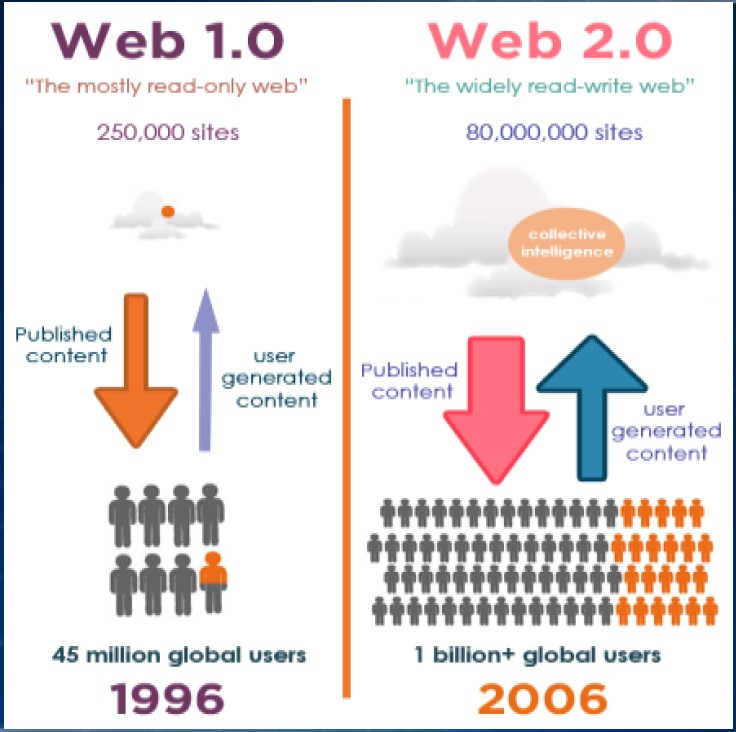
\includegraphics[width=0.75\linewidth]{images/06_lez_fig_01.jpg}
\end{figure}

Nel 1996 gli utenti globali di internet erano 45 milioni, nel 2006 a distanza di dieci anni oltre un miliardo di utenti di internet e anche la gestione dei contenuti è cambiata. I contenuti pubblicati da soggetti specializzati rispetto ai contenuti generati dagli utenti hanno un rapporto completamente diverso nel 1996 e nel 2006. Anche i siti presenti sul web 250 mila nel web 1.0, 80 milioni nel web 2.0. Si vede la grandissima differenza che nell'arco di dieci anni ha caratterizzato il rapporto dei cittadini con il web.\par
Per stare sul web occorre un dispositivo, i dispositivi oggi che consentono di approcciarsi al web sono innumerevoli, parliamo di tablet, di smartphone, di pc, di laptop e poi occorre un luogo su cui inserire i contenuti. Questo luogo può essere un sito creato da altri oppure un proprio sito e per avere un proprio sito occorre assicurarsi un dominio e per questo ci si rivolge ad un provider che generalmente offre servizi legati all'apertura del dominio ma anche altri servizi come un indirizzo email e lo spazio web necessario per creare il proprio sito.\par
Ricorderete dalle lezioni precedenti che il dominio è raggiungibile attraverso l'indicazione di un codice numerico ma che nel contesto del web questo codice numerico è sostituito da un nome vero e proprio, in maniera tale da semplificare e facilitare all'utente il ricordo di qual è la destinazione che vuole raggiungere.\par
Per poter effettuare la registrazione di un dominio, deve esserci un fornitore e questo deve essere riconosciuto come registrar ufficiale. Tutti i registrar che si occupano di domini.it lavorano insieme al NIC italiano, il registro .it, che è l'organo di registrazione centrale di tutti gli indirizzi italiani. Il NIC italiano fa riferimento all'ICANN che coordina la distribuzione dei domini di tutto il mondo.\par
Entrambe queste organizzazioni e le altre organizzazioni che sono attori all'interno del web, come operano davvero e come funziona concretamente l'assegnazione dei domini?\par
Riprendiamo quindi adesso più nel dettaglio un argomento che abbiamo iniziato ad affrontare in una lezione precedente.\par
\section{ICANN}
ICANN è l'Internet Corporation for Assigned Names and Numbers ed è responsabile per l'assegnazione e la gestione degli indirizzi web di primo livello, i General Top Level Domain. ICAN coordina tutti gli indirizzi web esistenti e assicura che ogni dominio sia unico, identificabile in maniera inequivocabile e raggiungibile attraverso un browser. Tuttavia non si occupa direttamente dell'assegnazione di questi indirizzi.\par
\begin{itemize}
    \item E' stato istituito nel 1998 su incarico delle autorità governative degli USA.
    \item ICANN oggi è un ente di gestione internazionale del quale fanno parte diverse entità non solo americane ma anche europee.
    \item ICANN, come detto, ha l'incarico di assegnare gli indirizzi IP e identificare e gestire i General Top Level Domain nel mondo.
    \item
\end{itemize}
\par
ICAN è coadiuvato da altri soggetti in particolare il NIC Registry.

\subsection{NIC Registry}

\begin{itemize}
    \item NIC Registry ovvero Network Information Center o Domain Name Registry che sono autorizzati da ICANN
    \item Si tratta di Naming Authorities che:
          \begin{itemize}
              \item gestiscono la registrazione dei domini locali o di secondo livello che sono
              \item responsabili del servizio WHOIS
          \end{itemize}

\end{itemize}

Ricorderete che i domini generali di secondo livello sono i Country Code Top Level Domain e sono quelli caratteristici dei diversi paesi nel mondo. Quindi abbiamo .it, .fr, .uk a seconda del paese di appartenenza a cui fanno riferimento. \par
I Registry associano gli indirizzi numerici necessari per muoversi in rete che sono lunghi e difficili da memorizzare con un nome. I registry a loro volta sono supportati da altri soggetti.
\subsection{Domain Name Registrar}
I Domain Name Registrar sono partner del NIC e si occupano della registrazione del dominio.
Provvedono a chiedere i dati relativi al registrante e li raccolgono in un database, il database proprio dei nomi di dominio e questo database contiene tutte le informazioni relative a coloro che chiedono e ottengono la registrazione di un nome di dominio. Il database che contiene i dati dei registranti può essere consultato attraverso un servizio che si chiama WHOIS (chi è).

I Domain Name Registrar
\begin{itemize}
    \item gestiscono la registrazione dei nomi locali o di secondo livello
    \item sono responsabili del servizio WHOIS
    \item
\end{itemize}{}

Per quanto riguarda l'Italia, il riferimento di ICANN è il registro.it.
\subsection{registro.it}
Il registro .it:
\begin{itemize}
    \item stabilisce in autonomia i criteri di assegnazione dei domini IT
    \item gestisce e amministra i top level domain .it
    \item gestisce i nomi dei server che consentono la raggiungibilità dei siti web .it
\end{itemize}

Il registro è gestito dal Consiglio nazionale delle Ricerche e ha sede presso l'Istituto di Informatica e Telematica del CNR di Pisa, del Centro nazionale delle Ricerche di Pisa.\par
Il registro .it è l'anagrafe dei domini .it, la targa internet dell'Italia. Soltanto attraverso di esso è possibile richiedere, modificare o cancellare uno o più domini .it.\par
Il registro.it:
\begin{itemize}
    \item come tutti i domini nazionali, si affida a registrar autorizzati
    \item gestisce il database dei nomi assegnati
    \item offre il servizio WHOIS .it
\end{itemize}

Attraverso il servizio WIS si ottengono informazioni sulla disponibilità del dominio e sul suo eventuale proprietario. In questo modo sono messi a disposizione del server di tutti i domini che hanno la stessa estensione insieme ai loro indirizzi IP.
%%11:37
\subsubsection{3WC Consortium}

Un altro attore del web è il 3WC Consortium, il World Wide Web Consortium. Si tratta di un'organizzazione internazionale nata nel 1994, è un'organizzazione non governativa ed è nata presso il MIT, il Massachusetts Institute of Technology, inventata dal padre del web, Tim Barners-Lee, in collaborazione con il CERN. \par
Il 3WC ha come scopo quello di sviluppare le tecnologie che garantiscono l'interoperabilità, le specifiche tecniche, le guideline e le linee guida delle applicazioni. L'obiettivo è quello di portare il World Wide Web al massimo del suo potenziale, agendo da forum internazionali con comunicazioni e attività comuni. \par
La composizione del 3WC Consortium è molto variata, è composto da aziende informatiche multinazionali di diversi settori, università e centri di ricerca. È inoltre un soggetto a cui compartecipano gli Stati Uniti e l'Unione Europea. \par
Il 3WC Consortium ha l'obiettivo di garantire il libero accesso al web. Per riuscirci è necessario, come detto, elaborare dei criteri comuni di utilizzo, un linguaggio comune condiviso di utilizzo, perché se ci fossero linguaggi diversi sarebbe ovviamente difficile poter interagire. Quindi il 3WC promuove:
\begin{itemize}
    \item standard tecnici comuni
    \item interoperabilità
    \item sviluppo di nuovi linguaggi
\end{itemize}

L'importanza dei membri del 3WC Consortium è tale che ne fa un organismo di grande autorevolezza.


\subsubsection{utenti del web 2.0}
Gli ultimi attori del web ma determinanti nel web 2.0, sono gli utenti.
Gli utenti del web 2.0 hanno a disposizione strumenti che con la loro duttilità e semplicità d'uso sono a disposizione dell'utente non esperto per consentirgli di operare. Sul web 2.0 molti nuovi servizi, la gran parte gratuiti, generano degli strumenti mediatici di grande potenzialità. Il loro utilizzo non richiede alcuna competenza specifica. Alcuni di questi servizi sono sviluppati interamente dagli utenti e non più dai tecnici e quindi hanno cambiato completamente pelle.

Vediamo adesso un breve video per riepilogare in qualche modo quello che abbiamo detto fino ad ora.
\par
\textit{Nel video si parla dell'interazione utenti web 2.0 (Facebbok, Twittwr, youtube, ecc) e della possibilità di fare marketing. E' molto breve.}\par

Avete visto quali sono gli strumenti messi a disposizione al giorno d'oggi, ma cerchiamo di capire un po' più nel dettaglio. \par
Gli utenti possono utilizzare una serie di strumenti diversi:
\begin{itemize}
    \item Wiki sono sistemi sviluppati e modificati liberamente dagli utilizzatori. Il caso esemplare di questo tipo di servizi è rappresentato da Wikipedia, l'enciclopedia libera sulla quale ogni utente iscritto può generare contenuti e che possono essere modificati e implementati da chiunque abbia accesso. Si tratta di un'enciclopedia libera e gratuita che nel bene o nel male è diventata un punto di riferimento per tutti coloro che fanno ricerche in rete ed è come detto interamente redatta dagli utenti che la utilizzano
    \item I CMS, Content Management System, sono dei sistemi di gestione dei contenuti multimediali e sono dei modelli di siti web preconfezionati per i quali basta scegliere un tema grafico da utilizzare e poi appunto riempirlo di contenuti. I CMS dispongono anche di funzionalità avanzate come la gestione degli utenti iscritti al blog e la gestione dei loro commenti e degli articoli pubblicati da altri
    \item I Feed RSS sono aggregatori di notizie, di articoli su argomenti specifici, di account email, di commenti sugli articoli dei blog e così via. Raccolgono le informazioni su vari siti differenti. Quando si avviano o vengono aggiornati questi programmi, le pagine web che ci interessano, già predisposte per l'uso, trasferiscono sul lettore Feed RSS una lista di articoli alla quale è possibile accedere rapidamente.
    \item I Cloud Computing. Il Cloud Computing è un insieme di tecnologie e di servizi che ci consentono di memorizzare i nostri dati, dati che utilizziamo per lavorare e quant'altro su un archivio multimediale, un archivio che è esterno al nostro computer e che risiede su un server da qualche parte nella rete internet. Con questa tecnologia tutti i documenti che elaboriamo vengono conservati su uno spazio web personalizzato senza occupare la memoria dei dispositivi che sono a nostra disposizione per l'archiviazione dei dati e senza impegnare il nostro sistema operativo. Il cloud permette di lavorare senza installare alcun software e di usufruire dei programmi e di altre risorse di cui abbiamo bisogno direttamente usando la rete. Il cloud, così come alcuni degli altri strumenti che sono a disposizione, hanno delle caratteristiche che possono anche presentare delle difficoltà ma ci occuperemo in una prossima lezione di quali sono le questioni più strettamente giuridiche collegate a questi sistemi.
    \item I social media sono gli strumenti di comunicazione sulla rete più diffusi in assoluto e più utilizzati e consentono l'interazione tra un grandissimo numero di utenti, tra i più noti Facebook che ha fatto in qualche modo da padrone nell'arco di dieci anni e che nella primavera del 2018 è stato coinvolto in uno scandalo molto grande, con molti effetti, che è il cosiddetto scandalo Cambridge Analytica e che ha riguardato la creazione e l'utilizzo di falsi profili su Facebook rubati da persone vere ed esistenti con finalità che erano collegate alle elezioni del presidente Trump negli Stati Uniti nel 2017. Ma anche di questo parleremo in una prossima lezione meglio.
\end{itemize}

\textit{Lo scandalo dei dati Facebook-Cambridge Analytica[1] è stato uno dei maggiori scandali politici avvenuti all'inizio del 2018, quando fu rivelato che Cambridge Analytica aveva raccolto i dati personali di 87 milioni di account Facebook senza il loro consenso e li aveva usati per scopi di propaganda politica.[2] È stato definito come un momento di spartiacque nella comprensione pubblica del valore dei dati personali e di conseguenza, provocando un forte calo del prezzo delle azioni di Facebook, si è chiesto una regolamentazione più rigorosa sull'uso dei dati personali da parte delle aziende tecnologiche.[3]
    Lo scandalo scoppiò a marzo 2018 a causa delle rivelazioni di un whistleblower, un ex dipendente della Cambridge Analytica, Christopher Wylie.}



Vediamo adesso però qual è la penetrazione nel mondo al giorno d'oggi, nel 2018.

\begin{figure}[ht]
    \centering
    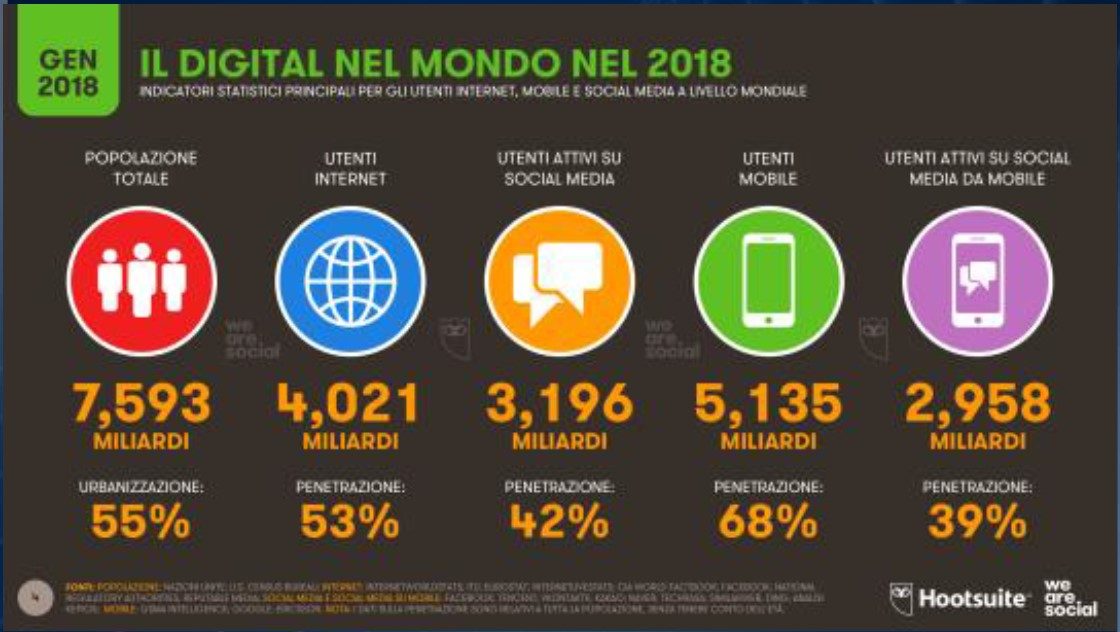
\includegraphics[width=0.75\linewidth]{images/06_lez_fig_02.jpg}
\end{figure}

Il digital nel mondo del 2018. Ecco qui da questo studio del 2018 potete vedere la penetrazione della rete nella popolazione totale. Abbiamo una popolazione totale di 7 miliardi e mezzo di persone, un'urbanizzazione del 55\% e 4 miliardi e abbondanti di utenti internet con una penetrazione del 53\%. \par
Tra gli utenti di internet attivi sui social media sono più di 3 miliardi, utenti mobile sono più di 5 miliardi e utenti sui social media da mobile sono quasi 3 miliardi. \par

\begin{figure}[ht]
    \centering
    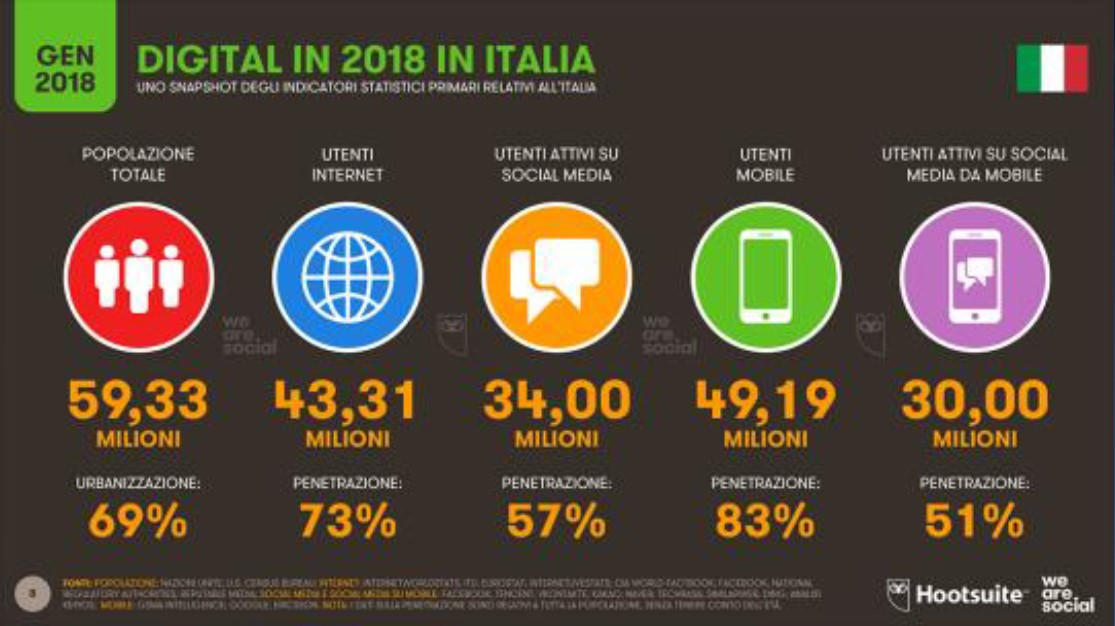
\includegraphics[width=0.75\linewidth]{images/06_lez_fig_03.jpg}
\end{figure}

In Italia dal gennaio 2018 abbiamo delle percentuali di presenza sul web estremamente elevate. Su 59 milioni di popolazione locale abbiamo 43 milioni di utenti internet. \par
Quindi come potete vedere ormai nel 2018 internet è diffuso ovunque. Se pensate a come era la situazione nei primi anni 90 dello scorso secolo, ricorderete abbiamo esaminato una timeline in una delle precedenti lezioni nelle quali proprio si comprendeva qual è stato il passaggio per il mondo moderno dall'epoca degli inizi di internet fino a oggi al web 2.0. \par
Potete rispondere ad una domanda. Come è cambiato il ruolo dell'utente nel web 2.0?

\subsection{Contestazione dei nomi a dominio.}
\subsubsection{Regole di assegnazione dei nomi a dominio}
Passiamo ad un altro argomento. Il nostro argomento adesso è contestazione dei nomi a dominio.
\subsubsection{Regole di assegnazione dei nomi a dominio}
La regola di base è first come first served, ma questa regola non tiene conto del fatto che può esserci un problema:
\begin{itemize}
    \item di diritto d'autore
    \item o può esserci un diritto all'uso del nome o della denominazione che non è quello di chi cerca di registrare il dominio.
\end{itemize}
Il registro infatti non fa delle verifiche sulla effettiva titolarità del nome che si vuole registrare.   \par
Se le regole sono violate, la persona che ha diritto ad utilizzare un determinato nome e che si rende conto che è stato utilizzato da altri ha degli strumenti diversi per riottenere l'assegnazione del nome a dominio a se stesso.\par

Perché un principio di chi primo arriva meglio alloggia è utilizzato sul web? Per una questione da un lato di praticità e rapidità, dall'altro perché come avete visto i domini sono assegnati da diversi registrar e quindi diventa estremamente difficile poter verificare se chi fa la richiesta di registrazione ha dei diritti effettivi e non calpesta invece i diritti degli altri. Nella registrazione è comunque richiesto di autodichiarare di avere i diritti per utilizzare quel determinato nominativo ma una verifica non viene fatta. Cosa può fare l'utente? L'utente può contestare il nome a dominio.

\subsubsection{Contestare i nomi a dominio}

L'assegnazione di un dominio dunque può essere controversa tra diversi soggetti.
\begin{itemize}
    \item Può esserci un diritto prioritario sul nome a dominio legato a un marchio registrato , all'esistenza di un determinato cognome e così via
    \item è possibile invece che il titolare del dominio lo abbia registrato utilizzando il nome a fini speculativi o abusivi
\end{itemize}

%24:31
Come contestare i nomi a dominio?
\begin{itemize}
    \item Esistono procedure di contestazione regolate e gestite dai registri locali
    \item devono tener conto dell'applicazione della normativa locale
    \item
\end{itemize}

Per contestare i nomi a dominio è possibile fare una \textbf{opposizione} che consente l'accesso a due procedure alternative al ricorso alla magistratura per la risoluzione della controversia. \par
L'opposizione di per sé non permette la riassegnazione automatica del dominio già registrato da altri però consente di attivare questo processo che è un processo stragiudiziale per ottenere e far valere le proprie ragioni. \par
Quindi contestare i nomi a dominio comporta la possibilità di fare una opposizione a cui segue:
\begin{itemize}
    \item un arbitrato irrituale
    \item oppure una procedura di riassegnazione
\end{itemize}

Al termine della procedura viene effettivamente riassegnato il dominio. \par
L'arbitrato irrituale consiste nell'affidare ad un collegio di persone esperte nell'assegnazione dei nomi a dominio la questione lasciando a loro di valutare, sulla base di una rapida istruttoria, chi abbia effettivamente il diritto di utilizzare quel determinato nome. Per poter accedere a questa procedura il registrante deve però aver sottoscritto la clausola arbitrale. \par
La procedura di riassegnazione invece anche questa è condotta da soggetti privati, sono degli studi professionali chiamati prestatori del servizio di risoluzione delle dispute (PSRD) e ha anche qui lo scopo di verificare che il dominio non sia stato registrato e mantenuto in mala fede. L'unico esito della procedura è la riassegnazione del dominio al soggetto che ha iniziato l'opposizione.\par

Per la gestione delle dispute ogni registro adotta delle regole simili. Per quanto riguarda l'Italia è il registro.it che provvede alla non solo all'assegnazione dei nomi di dominio ma anche a dirimere le controversie, per quanto riguarda l'Europa le informazioni sulla riassegnazione dei nomi a dominio e sulle procedure di opposizione si trovano sul sito di eurid.eu.it.\par

Lo spunto di riflessione di questa parte della nostra lezione è quali procedure si possono attivare per contestare un nome a dominio.it?

\section{Le regole di netiquette}

Le regole di netiquette. Alle origini e per lungo tempo internet non era regolato in alcun modo. Ricordiamo ancora una volta che alle origini e per i primi anni l'accesso a internet era possibile ad un numero limitato di utenti che erano sostanzialmente esperti o appartenenti a determinate categorie. Ma già dall'inizio degli anni 90 dello scorso secolo vi è stata l'apertura agli utenti comuni con un conseguente aumento di presenze sulla rete. Siamo passati dall'internet al web e così via. E' stato avviato un percorso che ancora non si è concluso.\par
Nei primi anni appunto non c'era nessun tipo di regolamentazione sul web ma l'esigenza di qualche forma di regolamentazione fra gli utenti si è sentita quasi dalle origini.\par
La netiquette consiste in un insieme di regole di buona educazione in rete. Come nasce questa parola? Da net (network, rete) e etiquette (buona educazione in lingua francese). La netiquette non è un regolamento imposto dall'esterno ma è una forma di autoregolamentazione degli utenti che ancora oggi valida anche se nel frattempo alcune norme sono state elaborate.\par
La netiquette, le regole di buona educazione sono sempre valide e sono sempre applicabili anche se non spesso utilizzate.\par
\textbf{La netiquette è un insieme di regole informali che disciplinano il buon comportamento dell'utente di internet (nel rapportarsi con gli altri utenti).}\par

\subsection{RFC 1855}
Come sono nate queste regole? Nel 1995 fu fatto una richiesta di commenti pubblicata, request for comment (RFC). Queste regole sono costituite da:

\begin{itemize}
    \item buona prassi
    \item vietano comportamenti scorretti
    \item vietano la commissione di reati
\end{itemize}

Sono ancora reperibili sul sito dove in origine sono state pubblicate. (https://tools.ietf.org/html/rfc1855) netiquette guidelines.\par

\subsubsection{il buon netizen}

Nel rfc 1855 sono elencate tutte le regole che permettono di diventare un buon netizen.\par
Quali sono le regole che deve rispettare?
Bisogna distinguere i vari tipi di comunicazione:
\begin{itemize}
    \item Comunicazione a uno a uno (post elettronica e dialogo)
    \item Comunicazione uno a molti tramite blog, social network, instant messenger
    \item servizi di informazione più generali
\end{itemize}

Le regole di base:
\begin{itemize}
    \item non appropriarsi di contenuti di altri
    \item non pubblicare il contenuto di un messaggio e email senza consenso
    \item non fare spam
    \item non violare la sicurezza
    \item non violare la privacy
    \item non compromettere il funzionamento della rete
\end{itemize}

Come potete notare si tratta di regole che in gran parte sono comunque presidiate da norme internazionali e nazionali, sia la tutela della privacy, sia la tutela rispetto alla commissione di crimini informatici, sia la tutela del diritto d'autore e così via. La maggior parte delle regole del buon vivere civile sulla rete sono regole che hanno un presidio offline forte con delle norme nazionali e internazionali e che quindi rispettare le regole di buona educazione porta anche a rispettare le leggi.\par
Oltre a queste regole di base ci sono delle indicazioni specifiche legate al tipo di interazione. \par
Nell'interazione da uno a uno:
\begin{itemize}
    \item si suggerisce nel testo di limitare l'uso del maiuscole e del grassetto
    \item si suggerisce di avere sintesi evitando divagazioni inutili
    \item si suggerisce di inviare le proprie comunicazioni a dei destinatari limitati e effettivamente necessari
\end{itemize}

Il suggerimento è quello di evitare di urlare sul web come può accadere invece con l'abuso di strumenti di evidenziazione e di richiamo.\par
Nel caso dell'interazione da uno a molti:
\begin{itemize}
    \item si parla di newsgroup e liste di distribuzione e si suggerisce di leggere prima di scrivere
    \item limitare e fare attenzione a ciò che viene inviato in cc e in ccn, in copia evidente e in copia nascosta. Ad esempio è opportuno utilizzare il ccn che non permette a tutti gli altri di conoscere gli indirizzi di posta elettronica della lista di destinatari per questioni di riservatezza.
    \item Si suggerisce di fare citazioni chirurgiche, fatte bene e con indicazione della fonte
    \item evitare guerre di opinioni in rete
    \item non inviare messaggi pubblicitari inutilmente
\end{itemize}

Anche in questo caso le regole sono abbastanza semplici, non sempre vengono ricordate. Negli anni 2017-2018, questa attenzione alle regole del vivere comune a volte sembra essere stata dimenticata. \par

Nei servizi di informazione occorre fare delle verifiche:

\begin{itemize}
    \item il servizio è gratuito oppure no
    \item qual è la fonte e quali sono le regole locali
    \item
\end{itemize}
\par
Nei social network:

\begin{itemize}
    \item attenzione alle bacache degli altri
    \item attenzione alla pubblicazione di fotografie
    \item attenzione al tagging
\end{itemize}

Insomma per stare correttamente in rete è suggerito di pensare due volte prima di reagire, \textbf{think twice before reacting}, anche se non tutti lo fanno. \par
Il nostro spunto di riflessione: quali sono le regole principali della netiquette?\par
Riepilogo degli spunti di riflessione, come è cambiato il ruolo dell'utente nel web 2.0, quali procedure si possono attivare per contestare un nome a dominio.it, quali sono le regole principali della netiquette?
\chapter{Lezione 7 - Internet e diritti umani - I parte}

Gli argomenti della lezione di oggi sono:
\begin{itemize}
    \item i diritti umani fondamentali  
    \item Internet e rivoluzione della comunicazione 
    \item Internet e violazione di diritti
\end{itemize}

\section{I diritti umani fondamentali}
I diritti umani fondamentali sono stati individuati all'indomani della Seconda Guerra Mondiale in diversi trattati e atti internazionali e nella Costituzione italiana. 
\begin{itemize}
    \item La Dichiarazione universale dei diritti umani (ONU 1948) 
    \item la Convenzione europea dei diritti umani (CEDU 1950) 
    \item la Carta dei diritti fondamentali dell'Unione europea del (UE 2000)
    \item la Costituzione italiana del (1948)
\end{itemize}

Si tratta di atti che rivestono un'importanza fondamentale per quelli che sono i principi generali a sostegno del nostro ordinamento. \par

\subsection{Libertà di espressione}
Libertà di espressione sancita dall'Art. 19 della Dichiarazione ONU, dall'Art. 10 CEDU, dall'Art. 11 della Carta UE e dell'Art. 21 della Costituzione italiana. \par
Fra i diritti fondamentali c'è ne uno in particolare che ci interessa per quello che riguarda Internet oggi ed è il diritto alla libertà di espressione e di comunicazione. Questo diritto è sancito dall'Art. 19 della Dichiarazione dell'ONU che dice che ogni individuo ha diritto alla libertà di opinione e di espressione incluso il diritto di non essere molestato per la propria opinione e quello di cercare, ricevere e diffondere informazioni e idee attraverso ogni mezzo e senza riguarda ad alcuna frontiera.\par
Negli stessi termini si esprime la Convenzione europea dei diritti dell'uomo che ribadisce il diritto alla libertà di espressione di ognuno, diritto che comprende la libertà di opinione e la libertà di ricevere e comunicare informazioni e idee senza ingerenze da parte delle autorità pubbliche e senza limiti di frontiera. \par
La Convenzione dei diritti dell'uomo però aggiunge che l'esercizio di queste libertà poiché comporta doveri e responsabilità può essere sottoposto a formalità, condizioni, restrizioni e sanzioni che sono previste dalla legge e che costituiscono misure necessarie in una società democratica alla sicurezza nazionale, all'integrità territoriale, alla pubblica sicurezza, alla difesa dell'ordine, la prevenzione dei reati, alla protezione della salute e della morale, alla protezione della reputazione dei diritti altrui per impedire la divulgazione di informazioni riservate o per garantire l'autorità e l'imparzialità del potere giudiziario.
\par
Ecco quindi che la Convenzione europea introduce un contemperamento fra il diritto di libera espressione e altri diritti. \par
La Carta dei diritti dell'Unione europea ribadisce il diritto di ogni persona alla libertà di espressione, ribadendo che questa libertà include la libertà di opinione ma anche la libertà di ricevere informazioni. \par
Negli stessi termini l'articolo 21 della Costituzione italiana prevede tra le altre cose che soltanto in casi eccezionali sia possibile disporre il sequestro di stampati.\par
Ovviamente questi diritti sono stati individuati in un momento storico nel quale il principale mezzo di espressione era la carta stampata e quindi non si poteva all'epoca tenere in conto di quelle che sono le caratteristiche che oggi abbiamo con Internet.

Libertà di opinione e di ricevere e comunicare informazioni e idee senza ingerenza di autorità pubbliche e senza limiti di frontiera. \par

Abbiamo visto che la libertà di espressione ha due aspetti. Il primo aspetto riguarda il diritto ad essere informati, il diritto a ricevere informazioni. Questo diritto è strettamente connesso con il diritto di cronaca, diritto dovere di cronaca, anzi quello che hanno i giornalisti nel momento in cui informano il pubblico di notizie che abbiano interesse pubblico e che per questo nell'esercizio di questo diritto di cronaca non possono essere limitati in alcun modo, non possono essere censurati. L'altro aspetto è il diritto di esprimere liberamente le proprie opinioni attraverso qualunque mezzo e questo aspetto del diritto della libertà di espressione è un aspetto che interessa particolarmente quando affrontiamo Internet.\par
Internet infatti è uno strumento che ha cambiato completamente il modo di comunicare perché consente a qualunque persona di esprimere la propria opinione senza la necessità di avvalersi di strumenti. \par
%05:48
Il diritto di esprimere liberamente il proprio pensiero deve essere contemperato con altri diritti: (la privacy, la reputazione, la pubblica sicurezza, la prevenzione dei reati, la tutela dei segreti).\par
La convenzione europea dei diritti dell'uomo ricorda che vi sono anche altri diritti fondamentali che devono essere rispettati nello stesso modo rispetto alla di libertà di espressione. Questo significa che anche nel momento in cui chiunque decida di comunicare le proprie opinioni attraverso internet dovrà comunque tener conto del fatto che vi sono altri tipi di diritti che si contrappongono alla libertà di espressione del proprio pensiero e che vanno comunque tenuti in considerazione. Immaginiamo ad esempio il fatto di raccontare al pubblico delle notizie riservate che riguardano terzi, ad esempio un segreto di stato, immaginiamo di utilizzare delle espressioni nel comunicare con il pubblico attraverso internet che sono diffamatorie perché sono lesive dell'onore e della reputazione di altri.\par
Spunto di riflessione di questa parte della lezione è chiedersi con quali altri diritti può interferire la libertà di espressione e comunicazione.

\subsection{internet e della rivoluzione della comunicazione}
Dopo 65 anni dalla Dichiarazione Universale dei Diritti Umani esiste un nuovo contesto. Internet rappresenta uno dei grandi strumenti di cambiamento. Come abbiamo detto nel momento in cui sono state promulgate le carte dei diritti fondamentali, il mondo era un mondo nel quale l'espressione delle proprie idee poteva essere veicolata attraverso strumenti che nella gran parte dei casi erano strumenti sottoposti ad una gestione. Immagino i giornali in particolare, ma lo stesso discorso vale anche con riferimento allo strumento televisivo. Si tratta di strumenti di comunicazione di massa a cui non tutti possono accedere per comunicare le proprie opinioni. Nel momento in cui si accede a questi strumenti di comunicazione di massa per comunicare qualche cosa, esiste una forma di valutazione preventiva effettuata da chi, l'editore, il giornalista, pubblica l'informazione e che quindi necessariamente filtra quelle che sono le informazioni che passano al pubblico.\par
Con l'utilizzo di internet è cambiato tutto. Internet è accessibile da parte di chiunque o meglio è in concreto utilizzato da una grandissima parte della popolazione mondiale e non ha alcun tipo di valutazione preventiva rispetto al contenuto, all'informazione, alla comunicazione che viene inserita. Questo significa che dall'altra parte chi riceve, chi si informa attraverso internet non ha alcuna possibilità di una valutazione preventiva rispetto alla qualità dell'informazione fornita, rispetto alla veridicità dell'informazione fornita, rispetto al fatto che l'informazione fornita sia un'informazione che non lede alcun altro diritto. Questo è un aspetto che va valutato con estrema attenzione.\par 
Più di un terzo della popolazione mondiale è connessa a internet, si parla di più di 600 milioni di famiglie (informazione da International Telecomunication Union, un rapporto del 2012 che probabilmente oggi è ancora diverso).\par
Il fatto che un numero così ingente di persone sia collegato ad internet è un segnale che lo strumento oggi riveste un ruolo importante per la comunicazione di massa. Quello che emerge dagli ulteriori approfondimenti che sono stati fatti è che nella maggior parte dei casi le persone utilizzano internet come strumento di carattere personale, per informazioni personali, per parlare della propria vita e soltanto in parte lo strumento è utilizzato per ragioni di carattere professionale o lavorativo.\par
In particolare le tecnologie dell'information and communication sono un fattore di crescita economica, di esportazione di investimenti in bene e servizi, specie nei paesi in via di sviluppo. Nei paesi nei quali le comunicazioni sono sempre state estremamente difficili, l'avvento di internet ha comportato dei cambiamenti notevoli anche nella gestione delle attività commerciali.\par
Esistono paesi del terzo mondo, in particolare ho in mente l'Africa, nei quali mancano moltissime cose ma esiste internet e questo consente anche ai piccoli produttori di far conoscere i propri prodotti ed eventualmente di mettere in moto un meccanismo di esportazione che può essere un fattore di crescita economica notevole. \par
Internet, anche attraverso l'utilizzo di email e social networks, è uno degli strumenti più utilizzati per comunicare. L'utilizzo dei social networks si è diffuso sostanzialmente negli ultimi 10 anni ed ha cambiato ancora di più la modalità di gestire la comunicazione di massa. Nei social network in particolare si proiettano gli interessi, le comunicazioni, i desideri della popolazione molto spesso su questioni di carattere squisitamente personale. Internet è  anche uno strumento di esposizione della persona che ha radicalmente stravolto le modalità di relazionarsi fra le persone come precedentemente la conoscevamo. I giovani che oggi si affacciano a internet sono nati all'interno del mondo digitale e questo non può non essere considerato anche in prospettiva futura.\par 
Spunto di riflessione di questa parte della lezione. Quale ruolo ha internet nel mondo moderno? Questa domanda è una domanda a cui occorre rispondere tenendo conto di tutti gli aspetti di cui si è parlato. \par

\subsection{internet e violazione di diritti}

Ora parliamo di internet e della possibilità che il suo utilizzo comporti la violazione di altri diritti. \par
Internet può trasformarsi in uno strumento di aggressione di altri diritti. Vi sono diverse situazioni concrete che si sono verificate negli ultimi anni e che ci fanno comprendere come internet possa essere uno strumento di aggressione di altri diritti, possa essere uno strumento che mette in difficoltà, che crea problemi e questo va gestito.\par
Molto spesso quando si parla di introdurre delle limitazioni, delle regole in internet, il popolo degli internauti si solleva contestando che vi possa essere un bavaglio al diritto di informazione, che vi possa essere un bavaglio alla libertà di espressione. Questo tipo di valutazioni, che sono valutazioni correnti, dovrebbero essere fatte con estrema attenzione anche perché spesso nel momento in cui si protesta rispetto alla possibilità di una limitazione del diritto di informazione, non ci si rende conto che chiunque può essere leso nei propri diritti proprio da questa stessa libertà.\par
Vi sono alcuni casi concreti di cui adesso parleremo che inducono certamente a riflettere.\par 
\subsubsection{Il caso Data Gate}
Nel caso Data Gate, così chiamato, la National Security Agency degli Stati Uniti ha raccolto un'ingente quantità di intercettazioni e dati geolocalizzati in tutto il mondo. Questo episodio del cosiddetto Data Gate è arrivato sulle cronache di tutti i giornali, di tutti i media nello scorso autunno. È capitato che la National Security Agency abbia raccolto un'ingentissima quantità di dati, di informazioni e intercettato comunicazioni relative alle attività più diverse, ma anche relative ad alcuni capi di Stato.\par
Su richiesta di informazioni, la NSA ha evidenziato che questa attività era stata svolta per la lotta contro il terrorismo. Quindi le ragioni per questa raccolta di dati erano delle ragioni estremamente rilevanti di sicurezza pubblica. Non c'è dubbio che la sicurezza pubblica è qualche cosa che deve essere tutelato alla pari della libertà di informazione. Tuttavia il problema che si pone è quali sono i limiti che questo modo di raccogliere informazioni debba avere.\par
L'ONU è intervenuta sul tema a tutela della privacy, cioè a tutela della riservatezza delle comunicazioni. L'impulso all'intervento è stato dato da alcuni Stati, in particolare il Brasile, che non hanno gradito un'interferenza da parte degli Stati Uniti nei propri affari di Stato.\par
Il tema importante in questo caso va oltre quelle che sono le relazioni tra singole persone, ma giunge proprio alla relazione fra gli Stati, relazione che per il momento è una delle relazioni più importanti per mantenere l'autonomia e la libertà di ogni singolo Stato. \par
\textbf{La raccolta di dati ha un aspetto legato al divieto di interferenze arbitrarie nella vita privata e nella corrispondenza che è un altro diritto fondamentale sancito dall'articolo 12 della Carta ONU, dall'articolo 8 della Convenzione Europea dei Diritti dell'Uomo, dagli articoli 7 e 8 della Carta dei Diritti dell'Unione Europea e per dall'articolo 15 della Costituzione Italiana.}\par
Abbiamo detto all'inizio di questa lezione che il diritto alla libertà di espressione, è uno dei diritti fondamentali enunciati dalle carte internazionali e dalla Costituzione Italiana. Ve ne sono altri che essendo diritti fondamentali sono alla pari della libertà di espressione. \par
Tra questi vi è proprio il diritto alla segretezza della corrispondenza e, con riferimento alle più recenti carte internazionali, particolare alla carta di Nizza, il diritto a tutelare la propria vita privata, la cosiddetta privacy, rispetto a qualunque tipo di interferenza esterna.\par
Nel caso dei mezzi di comunicazione di massa, la tutela della propria riservatezza rispetto a ogni interferenza esterna passa attraverso la possibilità di chiedere una limitazione delle informazioni che riguardano la persona stessa.\par
\subsubsection{il furto di identità}
L'utilizzo di dati personali può comportare la commissione di alcuni fatti che costituiscono reato per quanto riguarda la legge italiana. Innanzitutto il furto di identità che è colui si finge un'altra persona per ottenere vantaggi, ad esempio con l'accesso a conti correnti bancari, oppure per danneggiare la reputazione altrui, ad esempio con l'apertura di account di posta elettronica e con l'uso dei dati, ad esempio, su siti pornografici.\par
Questi fatti costituiscono reato. Il furto di identità costituisce reato nell'ordinamento italiano. Dal punto di vista concreto il furto di identità può comportare un depauperamento patrimoniale delle persone. Mi riferisco a quei casi nei quali vengono rubate le informazioni relative ad esempio all'accesso ai conti correnti bancari e vengono carpite queste informazioni attraverso diverse tecniche, chiamate fishing o in altri modi, tecniche le quali inducono in errore la persona che è titolare di quei dati, sono tecniche che fanno sì che la persona ingannata comunichi le proprie credenziali e poi queste credenziali vengono utilizzate da chi le ha raccolte per accedere al conto corrente bancario e svuotarlo.\par
Un altro esempio concreto estremamente diffuso è quello nel quale si utilizzano i dati, le informazioni relative ad una persona per danneggiarne la reputazione. Si tratta di casi che si sono verificati di frequente quando c'è un motivo di rabbia, di odio nei confronti di una persona, si utilizzano i suoi dati personali per aprire un account di posta elettronica e attraverso questo si fanno comunicazioni che mettono in cattiva luce la persona di cui i dati sono stati sottratti.\par
Uno dei reati che si possono contestare con riferimento al furto di identità è:


\begin{itemize}
    \item \textbf{reato di sostituzione di persona} prevista e punita dall'articolo 494 del nostro codice penale. 
    \item \textbf{reato di truffa} che è prevista e punita dagli articoli 640 e seguenti del codice penale;
    \item \textbf{reato di trattamento illecito di dati personali} previsto e punito dall'articolo 167 del Decreto Legislativo 196 del 2003 detto anche codice della privacy
\end{itemize}

\par

In che cosa consistono questi reati?\par
La sostituzione di persona è il fatto di chi assuma in qualunque modo l'identità di un altro per ottenere un vantaggio o per danneggiare qualcun altro. Si tratta di un reato che è previsto dal codice penale emanato nel 1930 e quindi stiamo parlando di un reato che teneva in conto delle modalità di realizzazione ben diverse da quelle che si utilizzano oggi su internet. Il caso poteva essere quello ad esempio del farsi rilasciare una carta di identità a nome di altri o anche semplicemente il fatto di farsi credere una persona diversa da quello che si è effettivamente con riferimento a titoli di qualunque genere qualifiche professionali, proprietà e quant'altro con l'obiettivo o di ottenere dei vantaggi oppure di danneggiare qualcun altro. L'obiettivo in questo senso non è rilevante, ciò che conta è il fatto di essersi sostituiti ad un'altra persona. Nel mondo di internet questo reato è assolutamente ipotizzabile anche se viene realizzato con modalità del tutto diverse. Come abbiamo detto il fatto di sostituirsi ad un altro su internet può avvenire attraverso l'utilizzo di credenziali altrui oppure attraverso l'apertura di account di qualunque genere a nome di altri utilizzando i dati di altri. Anche su internet questo reato può essere compiuto a proprio vantaggio per ottenere dei vantaggi oppure per danneggiare qualcun altro. A questo proposito occorre fare attenzione perché il fatto di danneggiare altri non è collegato necessariamente a un danno di carattere patrimoniale, può anche essere collegato ad un danno di carattere morale, ad una lesione di carattere morale.\par
Per quanto riguarda la truffa, il reato base è previsto e punito dall'articolo 640 del codice penale. Si tratta del fatto di chi utilizzando artifici e raggiri induce una persona in errore e lo induce a fare delle attività di disposizione di carattere patrimoniale a vantaggio proprio di chi commette il fatto o a vantaggio di un terzo. In questo caso quindi la truffa ha un collegamento diretto con un vantaggio di carattere patrimoniale. Gli artifici e i raggiri possono essere di qualunque genere purché abbiano come effetto di indurre in errore la persona che viene truffata.\par
Con riferimento ad internet il caso tipico è quello dell'utilizzo di credenziali altrui, anzi la raccolta di credenziali altrui attraverso degli artifici quali ad esempio il mandare un messaggio di posta elettronica apparentemente riconducibili all'Istituto Bancario presso il quale si ha il conto corrente. Questo artificio, questo inganno, l'invio della mail che apparentemente è riconducibile all'Istituto Bancario è un artificio che ha lo scopo di ingannare la persona a cui viene inviato e far sì che comunichi le proprie credenziali di accesso al conto corrente e questo consente di svuotare il conto corrente, quindi di sottrarre denaro al soggetto a cui fanno riferimento le credenziali.\par
Oltre a questa fattispecie di truffa il legislatore ne ha introdotta un'altra che è la cosiddetta truffa informatica prevista dall'articolo 640 ter del codice penale e introdotta negli anni 90 che prevede come reato il fatto di trarre in inganno, in questo caso il termine non è corretto, il computer. Nel caso è evidente che non si può ingannare il computer ma che l'utilizzo di questa formula significa che vengono utilizzati dei meccanismi per bypassare quelle che sono ad esempio le misure di sicurezza che proteggono un computer e ottenere in questo modo l'accesso al sistema.\par
L'ultimo reato che abbiamo introdotto è il trattamento illecito di dati personali previsto e punito dall'articolo 167 del decreto legislativo 196/2003 detto anche codice privacy. In questo caso si fa riferimento all'utilizzo di dati personali altrui in violazione di una o più norme previste dal codice stesso della privacy.\par
Il codice della privacy prevede in linea generale che ogni persona abbia diritto alla tutela dei dati che lo riguardano rispetto al trattamento da parte di altri. Come trattamento si intende qualunque tipo di attività venga svolta con questi dati a partire dalla raccolta, all'utilizzo, alla registrazione all'interno di una banca dati oppure all'utilizzo per qualunque tipo di attività. Il codice della privacy prevede che il trattamento di dati personali di terzi sia subordinato al consenso dell'interessato, cioè al consenso della persona a cui i dati fanno riferimento e che i dati raccolti siano utilizzati per scopi determinati e leciti. \par
Vi sono poi una serie di norme nel codice della privacy che disciplinano in maniera estremamente precisa e concreta le modalità di trattamento corretto dei dati personali. Nel caso in cui le modalità di trattamento corretto dei dati personali vengano violate e in particolare alcune delle norme previste dal codice non vengano rispettate, il codice prevede un reato che è quello del trattamento illecito. C'è però una condizione perché questo reato si possa effettivamente configurare e la condizione è che occorre che vi sia un trattamento effettuato a danno della persona a cui i dati fanno riferimento oppure che questo trattamento consista nella diffusione o nella comunicazione.\par
Questo secondo aspetto, cioè il trattamento illecito effettuato mediante la comunicazione e la diffusione, è quello che più interessa con riferimento ad internet. Diffusione infatti di informazioni significa comunicarle ad un numero indeterminato di persone. La pubblicazione di dati su internet che non sia una pubblicazione ristretta ad un gruppo chiuso e quindi accessibile da parte di soggetti non iscritti o che non fanno parte di questo gruppo, è una diffusione. Per fare un esempio concreto, la pubblicazione di dati, il postare dati su social network quali Facebook o altri, comporta una diffusione del dato e quindi se questa diffusione viene effettuata in violazione di quelle che sono le norme del codice della privacy, si ha trattamento illecito sanzionabile penalmente.\par
Da ricordare, con riferimento ai tre reati di cui abbiamo parlato, che le sanzioni per i reati sono sanzioni di carattere penale espressamente previste dall'ordinamento e quindi nel momento in cui l'autorità giudiziaria viene portata a conoscenza o vengono denunciati questi reati, l'autorità giudiziaria ha l'obbligo di procedere e quindi l'utilizzo dei dati su internet deve essere, sotto questo profilo, valutato con estrema attenzione. \par
Spunto di riflessione di questa parte della lezione riguarda quali sono i reati che possono essere commessi su internet. \par
Facciamo adesso un breve riepilogo degli argomenti di questa lezione.\par 
Abbiamo parlato dei diritti fondamentali, dei diritti umani fondamentali così come individuati dalle carte fondamentali internazionali e dalla Costituzione italiana. Tra questi diritti fondamentali vi è il diritto alla libertà di espressione e comunicazione che è un diritto che è sancito per quanto riguarda il nostro ordinamento dalla Costituzione italiana all'articolo 21, per quanto riguarda le carte internazionali è sancito dalla Dichiarazione universale dei diritti umani del 1948, dalla Convenzione europea dei diritti dell'uomo del 1950 e dalla carta dei diritti fondamentali dell'Unione europea del 2000.\par
Tutte queste carte internazionali e la Costituzione italiana affermano che è diritto fondamentale di ognuno quello di comunicare liberamente le proprie opinioni e quello di informarsi. Questo diritto è un diritto che va sempre con gli altri diritti fondamentali che sono sanciti ugualmente dalle carte dei diritti fondamentali e dalla Costituzione italiana. Questo significa che nell'esercitare il diritto alla libertà di espressione occorre tener conto degli altri diritti.\par
Il diritto alla libertà di espressione è un diritto che ha due aspetti, un aspetto passivo e un aspetto attivo. L'aspetto passivo è il diritto ad essere informati, di essere tenuti al corrente di fatti di rilevanza pubblica. Dall'altra parte c'è il diritto di esprimersi, il diritto di comunicare ad altri le proprie opinioni che è un diritto che ha acquisito una rilevanza del tutto nuova con l'avvento di internet. Internet infatti è uno strumento che consente a chiunque di esprimere la propria opinione di farla conoscere a chiunque altro, teoricamente in tutto il mondo.\par 
La comunicazione di informazioni, di notizie attraverso internet ha una caratteristica particolare che è quella di non avere limiti di tempo e di spazio, cioè nel senso che le informazioni pubblicate su internet risiedono senza nessun tipo di limitazione. Questo anche quando l'informazione stessa sia cancellata dal sito, dal luogo dove è pubblicata. Esiste infatti la possibilità di richiamare le informazioni in altro modo ed esiste la possibilità che esse vengano ridiffuse da terzi e in questo modo sostanzialmente non ci sono limiti alla comunicazione.\par 
Questo è un'innovazione che ha cambiato completamente i rapporti. Internet però può essere anche uno strumento proprio per le caratteristiche che ha di consentire la comunicazione e diffusione di informazioni senza limiti di tempo e di spazio. Internet può anche essere uno strumento che viola altri diritti. La comunicazione di informazioni senza alcuna autocensura, chiamiamola in questo modo, può portare alla violazione di altri diritti. In particolare possono essere commessi alcuni reati quali il furto di identità, nel caso in cui i dati di una persona vengono utilizzati su internet per parlarne male, per danneggiarla o per avvantaggiarsene. È possibile che vi sia la sostituzione di persona che è proprio il fatto di sostituirsi ad altri. È possibile che vi sia un trattamento illecito di dati personali quando si violano alcune specifiche norme del codice della privacy. Occorre quindi verificare con attenzione ciò che si fa.
\chapter{Lezione 8 -  Internet e diritti umani - II parte}

In questa lezione continueremo a parlare di Internet e diritti umani. Gli argomenti della lezione di oggi:
\begin{itemize}
    \item Internet e violazione di diritti
    \item la tutela dell'accesso a Internet
    \item la domanda se Internet sia o no un diritto fondamentale
\end{itemize}

\section{Internet e violazione di diritti}

Internet può trasformarsi in uno strumento di aggressione di altri diritti. Nella lezione precedente abbiamo iniziato a parlare del fatto che Internet è uno strumento di grande potenza, di grande utilità, ma può anche trasformarsi in uno strumento di violazione di altri diritti, che possono essere anche diritti fondamentali.\par

\subsection{Diffamazione}

La diffamazione è il comportamento che si commette quando si offende l'onore o la reputazione di qualcuno, in particolare in rete. Si tratta di un reato che è sanzionato dall'articolo 595 del codice penale e che ha come caratteristica quello di poter essere commesso in qualunque situazione. È sufficiente offendere l'onore o la reputazione di taluno parlando o scrivendo ad un numero indeterminato di persone in assenza del diretto interessato. Se questo reato viene commesso attraverso uno strumento di comunicazione di massa, nell'idea del legislatore del codice penale del 1930 erano i giornali, il reato è aggravato.

Internet indubbiamente è uno strumento di comunicazione di massa, anzi possiamo dire che è lo strumento principe di comunicazione di massa, perché è uno strumento che consente di arrivare ad un numero immenso di persone senza particolari difficoltà. Il fatto di offendere l'onore o la reputazione di taluno può a volte essere giustificato. Si tratta di quelle situazioni, in particolare che riguardano le notizie, le informazioni di carattere giornalistico, nelle quali l'offesa all'onore o la reputazione di taluno avviene raccontando fatti effettivamente accaduti, situazioni effettivamente esistenti che oggettivamente hanno come conseguenza quella di offendere l'onore o la reputazione.

\subsubsection{Diritto di cronaca}
In questi casi si parla di diritto di cronaca. Il diritto di cronaca riguarda specificamente i giornalisti e deve rispondere a dei principi, in particolare verità, continenza formale e continenza sostanziale.

Che cosa significa? Significa che fa parte della libertà di informazione, il fatto di raccontare delle notizie vere di interesse pubblico però anche facendo ciò che è necessario è che il modo di raccontare queste notizie corrisponda a dei criteri ben precisi che sono, oltre alla verità, anche una continenza formale, cioè una modalità espressiva, un linguaggio utilizzato che di per sé non ecceda, non trascenda rispetto a quelli che sono gli obiettivi di comunicazione, e una continenza sostanziale, cioè l'indicare delle notizie, delle informazioni, effettivamente necessarie per trasmettere la notizia. E quindi non condire le informazioni che si danno con delle informazioni non necessarie, con dei particolari non necessari, i quali, anche se potrebbero aumentare l'interesse della notizia, in realtà non sono essenziali per la trasmissione dell'informazione.

Vi sono dei termini, delle forme di espressione, che non aggiungono nulla, in particolare sono gli insulti e le oscenità che sono di scarsa utilità sociale e sono del tutto inutili per la verità. Già dagli anni 40 negli Stati Uniti si è ritenuto che ci sono alcune categorie di discorso ben definite e limitate la cui prevenzione e punizione non ha mai sollevato alcun tipo di problema nel rapporto fra diritto all'informazione e divieto di utilizzo di certe frasi. Si tratta proprio delle volgarità e delle oscenità, delle calunnie, degli insulti, di tutte quelle parole di scontro che per la loro stessa espressione comportano un danno, tendono a provocare la violazione dell'ordine pubblico e non hanno parte in alcun modo nell'esposizione di idee e sono di scarsa utilità sociale ai fini della verità che qualsiasi beneficio che ne potrebbe derivare è ampiamente superato da un interesse sociale più grande nell'ordine e nella moralità.

Queste parole erano state affermate dalla Corte Suprema degli Stati Uniti in una nota sentenza degli anni 40, ma i principi sono principi che sono assolutamente condivisibili e applicabili anche nel nostro ordinamento. Il fatto di avere come linea guida nelle modalità di espressione i principi del diritto di cronaca di cui si è parlato, cioè verità della notizia, continenza sostanziale e continenza formale consente di evitare di trascendere nelle comunicazioni che vengono fatte all'esterno.

C'è da dire che la pubblicazione di informazioni su internet ha degli effetti moltiplicatori del danno e quindi per questa ragione la cautela deve essere ancora maggiore. In particolare la pubblicazione di una notizia su internet \textbf{resta senza limiti di tempo}, non è sostanzialmente possibile cancellare le informazioni che vengono pubblicate su internet se non a prezzo di grandi difficoltà. Questo perché le informazioni pubblicate oltre ad essere contenute sul sito sul quale vengono pubblicate possono essere ritrasmesse e ripubblicate attraverso tutti i collegamenti che a quel sito possono essere fatti. E anche quando le informazioni vengono cancellate dal sito dove originariamente erano state pubblicate può accadere che siano in ogni caso reperibili su altre pagine, su altri siti.

Questo comporta \textbf{un'amplificazione del danno}, questo aspetto specifico che riguarda internet ha come conseguenza che la lesione dell'onore della reputazione eventualmente fatta attraverso internet può danneggiare l'interessato molto più a lungo di quanto non avvenga attraverso altri strumenti quali la carta stampata.
Un giornale viene pubblicato e poi viene dimenticato. Come abbiamo detto la pubblicazione di un'informazione su internet non ha questa caratteristica.

Un altro tema di particolare complessità collegato alla pubblicazione su internet è il \textbf{sistema della indicizzazione dei contenuti sui motori di ricerca}. Questo è un'altra specificità dello strumento che fa sì che anche una notizia vecchia e ormai superata nel tempo possa ritornare a galla per così dire attraverso le modalità di indicizzazione dei siti. Ed è accaduto in diverse situazioni che ad esempio la notizia di un procedimento penale a carico di una persona che ha come effetto quello di portare una lesione dell'onore della reputazione ancorché su fatti reali, è successo che notizie di questo genere abbiano continuato ad essere reperibili in modo semplice anche se nel frattempo il procedimento si era concluso con una assoluzione e quindi quella notizia relativa all'accusa in corso, non era più una notizia attuale ma anzi era una notizia superata da una notizia diversa.

Quindi ecco che la ragione per cui dover verificare con attenzione ciò che si pubblica su internet diventa essenziale.

\subsubsection{Responsabilità dei provider, dei blogger}

C'è da chiedersi a questo punto se vi sia una responsabilità dei provider, dei blogger, ovvero di tutti coloro che intervengono nella pubblicazione della notizia. L'autore, chi pubblica, non è l'unico soggetto che opera per la pubblicazione delle informazioni. La caratteristica di internet è che chiunque può trasmettere le informazioni ma per far questo comunque occorre lo strumento che è lo strumento gestito da provider, blogger e quant'altro. Quindi la domanda che ha suscita sempre un dibattito estremamente rilevante, i soggetti che concorrono nella trasmissione delle informazioni concorrono anche eventualmente nel reato di diffamazione unitamente a coloro che pubblicano?

C'è da dire che non esiste una normativa specifica su questo tema, esiste soltanto la \textbf{legge 70/2003} che è una legge che in recepimento di direttiva comunitaria prevede una responsabilità degli internet service provider soltanto nella misura in cui partecipano attivamente alla pubblicazione di determinati contenuti. Non c'è però alcun obbligo di controllo dei gestori, dei blogger, degli internet providers, assimilabile all'obbligo di controllo che invece la legge italiana prevede con riferimento alla carta stampata.

La normativa sull'editoria infatti prevede uno specifico controllo del direttore responsabile del giornale sugli articoli che vengono pubblicati. Questo non esiste su internet e da questa differenza di normativa sono nati una serie di dibattiti dottrinari e in ambito giurisprudenziale proprio per valutare in che termini e in che misura si possa invocare una responsabilità dei gestori dei blog e degli internet provider.

In linea di massima si può dire che il gestore del blog può essere ritenuto responsabile quando ha un effettivo potere di intervento rispetto alla pubblicazione. Ad esempio quando si è di fronte a un blog moderato. Ma in linea di massima si cerca di evitare un coinvolgimento del prestatore del servizio rispetto a quella che è l'attività che fa il singolo.

\subsubsection{Diritto all'oblio}

L'ultimo tema del profilo della diffamazione è il diritto all'oblio. Cos'è il diritto all'oblio? Il diritto all'oblio è il diritto ad essere dimenticati, è quel diritto che riguarda tutta la normativa in tema di protezione dei dati personali, in tema di riservatezza, ed è il diritto ad ottenere che le informazioni pubblicate, le informazioni conosciute che ci riguardano, siano informazioni effettivamente attuali.

Nel momento in cui, ed è il caso di cui si parlava prima, della pubblicazione di informazioni relative a procedimenti penali non più attuali, oppure la pubblicazione di notizie relative ad attività non più effettive, oppure la pubblicazione di notizie su persone che hanno cambiato la propria attività e che non desiderano più essere ricordati. Ecco, il diritto all'oblio è il diritto a far sì che ciò che transita sulla rete, ciò che transita in generale sui mezzi di informazione, siano notizie effettivamente attuali, effettivamente ancora di qualche interesse.

\subsubsection{Hate Speech}

Un altro tema che preoccupa con riferimento alle pubblicazioni di informazioni su internet è il cosiddetto hate speech.
Con Hate Speech si intende l'incitamento all'odio, all'intolleranza, alla discriminazione (razza, etnia, religione, genere, orientamento sessuale).

Hate speech è una espressione che è stata elaborata negli anni dalla giurisprudenza americana e che viene tradotta in italiano con la formula d'incitamento all'odio e indica quel genere di parole e di discorsi che hanno l'unica funzione di esprimere odio o intolleranza nei confronti di una persona o di un gruppo e che rischiano però di provocare delle reazioni violente contro quel gruppo o da parte di quel gruppo.

Nel linguaggio ordinario questa espressione indica un genere di offesa fondata su qualunque tipo di discriminazione ai danni di un certo gruppo. La condanna dello hate speech è condivisa anche se si pone, anche in questo caso, un tema di rapporto fra il diritto alla libertà di espressione e la tutela di altri interessi. Il tema è di grandissima attualità perché negli ultimi anni questa modalità di espressione si sta diffondendo sul web e quindi si sta verificando effettivamente un abuso del web per questo tipo di obiettivo.

Non esiste una normativa generalizzata a tutela di coloro che vengono colpiti dallo hate speech. Esistono azioni di vario tipo che vengono svolte sulla rete. 

Web e social networks in linea di massima hanno elaborato delle linee guida che sono diverse a seconda dei vari social networks. In particolare le grandi aziende come Google e Facebook hanno affidato la compilazione delle norme di utilizzo dei servizi a un gruppo di lavoro specifico, da questo gruppo di lavoro sono state elaborate le linee guida che sono consultabili agevolmente sui suddetti social network.

YouTube vieta esplicitamente lo hate speech inteso secondo una definizione generale di linguaggio offensivo di tipo discriminatorio. Facebook ha in linea di massima lo stesso principio però ammette che sia possibile pubblicare dei messaggi che abbiano dei chiari fini umoristici o satirici. E cioè si può trattare di un'offesa, si può trattare di un messaggio offensivo e aggressivo ma se viene fatto con un chiaro intento umoristico satirico non c'è più la necessità di rimuoverlo, è legittimato. Twitter non vieta esplicitamente lo hate speech e non lo cita nemmeno tranne in una nota sugli annunci pubblicitari in cui si specifica però che le campagne politiche contro un candidato generalmente non sono considerate hate speech.

Vale la pena di evidenziare che i grandi social network di cui stiamo parlando non sono radicati di base in Italia pur avendo generalmente delle sedi localizzate in Italia e quindi hanno come criteri ispiratori dei principi più che altro legati alla cultura giuridica e non solo degli Stati Uniti.

C'è da dire che non è semplice in concreto valutare tra i contenuti che vengono pubblicati quali sono semplicemente offensivi in quanto critici e quali invece hanno come possibile effetto quello di suscitare delle reazioni violente. E questo è un motivo per cui non è semplice effettivamente fare delle valutazioni.

In Italia si può consultare il sito nohatespeechmovement.org che è un sito promosso dalla comunità europea per sollevare il problema e sensibilizzare. E ancora in Italia proprio il sito nohatespeech.it che è un sito diretto alla sensibilizzazione. Questo nell'idea che la formazione, la sensibilizzazione e la cultura siano gli strumenti preventivi migliori rispetto a questo tipo di fenomeno.

Esiste dal punto di vista normativo la \textbf{legge 205/93} per la repressione dei crimini d'odio che prevede che vengano puniti tutti i reati commessi con finalità di discriminazione o di odio etnico, nazionale, razziale, religioso, ovvero per agevolare le attività di organizzazioni, associazioni o movimenti o gruppi che hanno tra i loro scopi le stesse finalità.

Questo principio, la finalità di odio ed discriminazione, costituisce un aggravante per i reati generali e costituisce un vero e proprio reato a parte nel caso di istigazione.

La \textbf{legge 38/2001} ha esteso alle minoranze linguistiche gli stessi principi già previsti dalla legge 205/93.

%20;50
\subsubsection{adescamento di minori}

Altro tema importante oggi su internet è quello che viene chiamato adescamento di minori. Consiste nell'\textbf{avvicinamento di bambini adolescenti a mezzo internet}. Questo avvicinamento avviene per scopi sessuali e avviene con un sistema di conquista della fiducia del minore che fa dei danni rilevantissimi. Il fenomeno è in aumento negli ultimi anni e questo aumento è agevolato dal fatto che anche i minori, anche i bambini molto piccoli, hanno la disponibilità degli strumenti di connessione alla rete. E' di tale portata che sono state costituite delle task force dedicate alla prevenzione e repressione di questo fenomeno.

In Italia questo condotta è considerata un crimine ed è prevista una specifica tutela per i minori dei 16 anni da parte \textbf{ dell'articolo 609 undiecis del codice penale}. Si tratta di una norma che è stata inserita a seguito della ratifica della convenzione di Lanzarote sulla tutela dei minori e che appunto prevede la punibilità di chiunque attraverso internet contatti un minore per gli scopi che sono stati detti.

La cosa interessante è che è sufficiente il tentativo, significa che non è necessario che ci sia effettivamente un contatto a seguito di questo adescamento ma già il solo fatto di raggiungere il minore per gli scopi che abbiamo detto attraverso lo strumento di internet è un reato.

L'obiettivo è quello di offrire una tutela penale ai minori di 16 anni che siano vittime di questi comportamenti seduttivi perpetrati attraverso mezzi di comunicazione a distanza. Il limite di età dei 16 anni è stato individuato tenendo conto della particolare fragilità dei ragazzi minori di quell'età. È evidente che se poi il contatto avviene e avvengono altri fatti esistono altre norme del codice penale per reprimerli.

Lo spunto di riflessione di questa prima parte della lezione è: quali cautele per pubblicare su internet?

\section{La tutela dell'accesso a internet}

Passiamo adesso al secondo argomento, la tutela dell'accesso a internet. Si è parlato a lungo in questa lezione e nella lezione precedente delle possibilità che internet offre, dei rischi in cui si incorre su internet, nel senso che internet può essere uno strumento di violazione di altri diritti. Occorre però chiedersi, e il mondo si chiede, le organizzazioni internazionali si chiedono in che termini e fino a che punto l'accesso a internet debba essere tutelato.

Nel rapporto ONU del 2011 si è evidenziato come internet sia un mezzo chiave per la libertà di espressione. Il relatore del rapporto ha chiarito con grande fermezza che poiché internet è diventato uno strumento indispensabile per realizzare una serie di diritti umani, la lotta contro la disuguaglianza e per accelerare lo sviluppo e il progresso umano, garantire l'accesso universale a internet dovrebbe essere una priorità per tutti gli Stati.

Questo si legge nel testo redatto da Frank Larue, il relatore speciale delle Nazioni Unite, che ha scritto un documento sulla promozione e la tutela del diritto alla libertà di opinione e di espressione. Quindi l'accesso a internet deve essere considerato una priorità per gli Stati.

Nel rapporto si richiama come dimostrazione di ciò che viene asserito la cosiddetta primavera araba nel Nord Africa e nel Medio Oriente, che è stata proprio agevolata dalla possibilità di essere collegati a internet. E tuttavia è anche certo che non in tutti gli Stati in questo momento internet sia effettivamente accessibile. In diversi Stati del Medio Oriente in cui internet è sottoposto a limitazioni, in altri Stati come l'Estonia, la Costa Rica, la Francia, che hanno dichiarato che internet è un diritto fondamentale. 

Quindi ci sono diverse posizioni da parte degli Stati, non c'è un approccio univoco e certamente non tutti gli Stati considerano come priorità assoluta il fatto di consentire l'accesso a internet.

È interessante però il fatto che nel rapporto di Frank Larue si riconosce che \textbf{è possibile introdurre delle limitazioni a internet. In particolare le limitazioni però devono essere eccezionali, legate a norme chiare e accessibili a tutti, e devono essere, laddove sono inserite, dirette a tutelare altri diritti di uguale rilevanza}. Ecco quindi che anche nel rapporto ONU ritornano gli stessi principi di cui abbiamo parlato, internet come strumento principe per veicolare la libertà di informazione, ma anche strumento che può avere delle conseguenze pericolose o dannose.

In quest'ottica è possibile introdurre delle limitazioni ma ciò che è fondamentale in paesi democratici, è che queste limitazioni siano delle limitazioni ben chiare, con delle finalità ben chiare e dirette a tutelare altri diritti fondamentali della stessa importanza, della stessa rilevanza, della libertà del diritto, della libertà d'espressione e che queste limitazioni siano introdotto con delle norme dello stato che devono essere estremamente chiare, accessibili a tutti e quindi facilmente individuabili.

Il fatto che nel rapporto si bilancino la libertà di espressione e delle possibilità di limitazioni, è conforme a quello che già avevamo potuto verificare nella lezione precedente dei principi sanciti dalle convenzioni internazionali, convenzione ONU, convenzione CEDU e costituzione italiana, rispetto alle possibili limitazioni del diritto alla libertà di espressione.

Lo spunto di riflessione è se internet sia in grado o meno di cambiare il rapporto fra libertà di espressione e altri diritti.

\subsection{Internet è un nuovo diritto fondamentale?}

Ultimo argomento di questa lezione è se internet è un nuovo diritto fondamentale. Alla luce di tutto quello che abbiamo potuto vedere, degli aspetti che abbiamo potuto esaminare, la domanda se internet di per sé sia o meno un diritto fondamentale è una domanda di estrema importanza.

I termini della questione sono: \textbf{l'accesso a internet è un diritto umano fondamentale di ultima generazione oppure è uno strumento che agevola il godimento di altri diritti?}

La questione non è una questione di soluzione semplice, certamente è un diritto fondamentale la libertà di espressione e l'abbiamo detto più volte. Certamente internet è uno strumento che consente di svolgere la libertà di espressione al massimo grado e quindi certamente avere l'accesso a internet consente di svolgere questo diritto fondamentale, ma da questo si può dedurre che l'accesso ad internet sia esso stesso un diritto?

Da ricordare che si suole dividere i diritti fondamentali in diritti di prima, seconda, terza generazione e così via. È chiaro che i diritti di ultima generazione, i diritti nuovi come questo sono dei diritti che si può pensare di tutelare soltanto dopo aver già garantito i diritti fondamentali primari.

Chi sostiene che l'accesso a internet sia un diritto fondamentale lo fa sul presupposto di una massima diffusione di internet, chi sostiene invece che internet sia soltanto uno strumento che agevola il godimento di altri diritti lo fa sul presupposto che internet in effetti è uno strumento e che internet in effetti non è diffuso ovunque e che non tutti gli stati, appunto come si diceva, hanno la stessa sensibilità rispetto al modo di fornire uno strumento.

Internet può essere, lo abbiamo detto, uno strumento attraverso cui violare altri diritti e quindi dato che si tratta di uno strumento che può essere usato positivamente ma anche negativamente, allora forse va considerato come uno strumento.

Le differenti opinioni possono essere facilmente individuabili anche tenendo conto di quelle che sono le normative che sono state adottate in diversi paesi. In Francia, alcuni anni fa, fu adottata la cosiddetta legge Hadopi che ormai è al tramonto che prevedeva l'obbligo per i fornitori di connettività, per i provider di sconnettere coloro che scaricavano musica o altri contenuti protetti dal diritto d'autore per più di tre volte. Quindi si dava agli internet service provider un obbligo di controllo che non è previsto in altri ordinamenti. 

Italia la cosiddetta legge Stanca considera un diritto per i disabili di avere l'accessibilità ai internet.

Nell'Unione Europea l'emendamento 138/46 in tema di diritto d'autore si occupa specificamente della violazione del diritto d'autore su internet.

Ecco quindi che gli aspetti che vengono trattati sono di vario genere.\par
Dal punto di vista dei fenomeni la primavera araba è stato proprio un esempio estremamente importante per il mondo per comprendere come l'utilizzo di internet nel bene e nel male abbia consentito di sviluppare una rivolta, un moto verso la libertà, verso un cambiamento di carattere democratico all'interno di quelle popolazioni. La maggior parte delle notizie che sono state comunicate, veicolate, che hanno consentito a quelle popolazioni di parlarsi e di andare avanti è stata resa possibile proprio dal web, proprio dalle comunicazioni su internet. E possiamo ricordare che ci fu durante la primavera araba proprio l'uccisione di un blogger proprio perché consentiva la comunicazione di informazioni che facevano sapere che cosa stava accadendo.

In periodi più recenti possiamo invece ricordare ciò che è accaduto e che sta accadendo in Turchia. Nel corso di quest'ultimo anno con l'avvicinarsi delle elezioni presidenziali è stata introdotta una legge di controllo all'interno della Turchia su internet e in particolare su youtube e twitter. Si tratta di norme che prevedono il controllo e che sono state ufficialmente motivate dalla necessità di reprimere violazioni e dalla necessità di tutelare dell'ordine pubblico.

In altri termini le ragioni che sono state date per l'introduzione di queste norme di carattere restrittivo sono delle ragioni che in astratto corrispondono a quei principi di cui abbiamo parlato prima riportati dal rapporto ONU. Ricordate che il rapporto ONU dice che riconosce la possibilità di introdurre delle limitazioni, purché queste limitazioni siano finalizzate a una tutela di altri diritti fondamentali, purché queste limitazioni siano introdotte con leggi ben chiare e comprensibili e accessibili a tutti. Il principio a cui si è fatto riferimento in Turchia era un principio di questo tipo.
%36:30
Quindi in teoria non c'era motivo per contestarlo. Il problema è che l'introduzione di queste limitazioni aveva come effetto quello di introdurre una forma di censura e quello che si è ritenuto motivo per l'introduzione di questa forma di censura era un motivo di carattere politico, un controllo sugli avversari politici.

In realtà questa normativa non ha resistito a lungo perché la Corte Costituzionale turca ha ordinato o ne ha dichiarato l'illegittimità consentendo la riapertura di YouTube e poi di Twitter. Quindi all'interno stesso della Turchia c'è stato un movimento di diritto che ha bloccato questi tentativi.

Per quanto riguarda la Turchia, c'è anche da dire che laddove dovesse effettivamente andare avanti la candidatura per l'ingresso all'interno dell'Unione Europea, la Turchia sarebbe comunque tenuta a rispettare quelli che sono i vincoli dettati dall'Unione Europea tra cui anche la tutela dei diritti fondamentali e quindi anche quello che riguarda la libertà di informazione. Non sarebbe più possibile introdurre delle limitazioni che nel resto d'Europa non sono ammissibili.

Ricordo il caso Data Gate di cui abbiamo parlato nella lezione precedente e che ricorderete è un caso nel quale vi è stata da parte della National Security Agency degli Stati Uniti la raccolta di informazioni che hanno riguardato diversi paesi e anche capi di Stato e rispetto ai quali c'è stata una presa di posizione dall'ONU.

Lo spunto di riflessione per quanto riguarda internet è libertà da una parte e governance dall'altra, come gestirli? Questa è la domanda che dovete porvi, questa è la domanda a cui è difficile rispondere e quindi si potrà ancora riflettere a lungo.
\chapter{Lezione 9 - Identità digitale}

Nella lezione di oggi parleremo di identità digitale. 

Gli argomenti della lezione di oggi:
\begin{itemize}
    \item identità digitale 
    \item identità digitale e pubblica amministrazione 
\end{itemize}

\textbf{L'identità digitale non è la semplice trasposizione elettronica di quella fisica.} \par
Per parlare di identità digitale occorre definire:
\begin{itemize}
    \item l'identità personale 
    \item l'identità digitale
    \item il processo tecnologico di identificazione
\end{itemize}

Si tratta di tre argomenti del tutto diversi anche se evidentemente ci sono dei collegamenti stretti.

\section{Identità digitale}
\subsection{Identità personale}

\textbf{L'identità personale è l'insieme dei caratteri fisici e psicologici che rendono una persona quella che è e diversa da ogni altra.} \par
Quando si parla di identità personale si fa riferimento ad una serie di elementi che sono stati individuati nel corso del tempo. L'identità personale è un insieme di caratteristiche che vengono anche prese in considerazione dall'ordinamento nei rapporti tra l'individuo e lo stato.\par
L'identità personale è un complesso di caratteristiche che rappresentano, che individuano la personalità. L'identità personale quindi è un coacervo, un insieme di elementi del tutto diversi che però individuano un soggetto, una persona come assolutamente unica.\par
Nel rapporto con lo stato vi sono diversi profili di tutela dell'identità personale:

\begin{itemize}
    \item l'individualità. L'identità personale tutelata è quella del singolo soggetto, del singolo individuo, diverso appunto da ogni altro. Il fatto di essere diverso e unico nel rapporto con gli altri è fondamentale per tutti quelli che sono i rapporti giuridici che vengono instaurati dalla persona con i consociati, coloro che vivono nello stesso ambiente.
    \item La fama. Un individuo può essere più o meno conosciuto nel gruppo dei consociati a cui fa riferimento e la sua fama, le modalità con cui è conosciuto sono per lui essenziali. 
    \item la credibilità
    \item la reputazione
    \item il credito inteso come rapporto con gli altri ma anche inteso come modalità di gestione di diritti, doveri e di attività nel rispetto alle altre persone.
\end{itemize}

Vicino al concetto di fama vi è la credibilità del soggetto e ancora la reputazione del soggetto. Queste due sono caratteristiche inscindibili che consentono di rappresentare l'individuo con se stesso e rispetto agli altri in un modo che è considerato più o meno positivo. Ognuno ha diritto a che la propria credibilità e la propria reputazione siano effettivamente quelle corrispondenti a ciò che l'individuo sente di essere.\par

Quindi in sintesi l'identità personale è un elemento caratterizzante di ogni persona ed è connesso alle garanzie che sono proposte dall'ordinamento, garanzie di carattere costituzionale e anche date da altre norme. In particolare si richiamano quelli che sono i principi del codice civile in tema di diritti della persona, in tema di individualità della persona. Si richiamano quelli che sono i principi sanciti dal codice penale per la tutela della persona rispetto non soltanto della persona fisica ma anche della persona come soggetto che ha una certa reputazione, una certa credibilità, una certa fama da difendere.\par
Da ultimo, nella più recente evoluzione, la tutela dell'identità personale è anche stata data con la tutela dei cosiddetti dati personali. La normativa, meglio nota come normativa tutela della privacy, si occupa proprio di difendere, di tutelare l'individuo rispetto a un utilizzo non corretto fatto dei dati personali che lo indicano, che lo individuano come soggetto unico al mondo nella gestione dei rapporti con gli altri.\par 
Individuata quella che è l'identità personale si tratta di verificare e di capire che cos'è l'identità digitale e in che rapporto l'identità digitale si pone rispetto all'identità personale. 

\subsection{L'identità digitale}
\textbf{L'identità digitale è la rappresentazione virtuale di un'identità reale che è utilizzabile nell'interazione elettronica.} 
%5:30

Ecco quindi che individuiamo immediatamente quella che è la prima caratteristica di un'identità digitale, la rappresentazione virtuale. L'identità digitale non è qualcosa di diverso rispetto all'identità personale, si tratta sempre della rappresentazione, dell'individuazione di una persona che ha una sua realtà. Quello che interessa in questa relazione è che l'identità digitale è l'elemento che è utilizzabile in una interazione elettronica, cioè sui rapporti che vengono instaurati nella gestione di relazioni elettroniche su internet e quant'altro. \par
Quali sono i legami con l'identità reale? \par
Si parla di anonimato o di possibilità di associazione tra le informazioni dell'identità digitale e la persona a seconda del modo in cui queste informazioni vengono proposte. Nel momento in cui le informazioni che individuano l'identità digitale sono delle informazioni che non consentono un facile collegamento con l'effettiva identità della persona, si può parlare di anonimato.\par 
Quando invece questi elementi di identità digitale sono degli elementi che consentono un'associazione più o meno ampia con l'individuazione della persona fisica c'è un legame che si può ritenere più stretto.\par
L'identità digitale può essere forte oppure debole.\par 
Questa distinzione tra identità forte e identità debole riguarda le caratteristiche distintive della persona individuata nel mondo digitale. Si parla di identità forte se questa identità digitale coinvolge un elevato numero di caratteristiche distintive. Si parla di identità debole se invece la descrizione dell'individuo contiene delle caratteristiche inferiori.\par
L'identità digitale è collegata con l'identità reale nella misura in cui consente l'accesso a servizi digitali da una parte e mette a rischio la privacy, la riservatezza della persona dall'altra.\par %8:35
L'accesso a strumenti, a servizi, a spazi nel mondo digitale è consentito attraverso l'identità digitale.\par
L'identità digitale è come detto che fa riferimento a informazioni di carattere personale. Quando si parla di informazioni c'è da dire che le informazioni personali possono essere replicate senza limiti e con una grande precisione. Quindi le informazioni che vengono utilizzate per costruire, per evidenziare, per individuare l'identità digitale sono informazioni che possono essere riprodotte nella costruzione di identità digitali diverse che consentono per esempio l'accesso ad altri servizi, ad altri spazi.\par
Un tema che si è posto frequentemente nei primi tempi in cui si parlava del rapporto fra identità digitale e identità personale è se si possa parlare di tante identità digitali quante sono le agglomerazioni di dati che consentono appunto di fare riferimento alla persona e che vengono utilizzate in varie situazioni.\par%10:13

In effetti non è corretto parlare di più identità digitali, l'identità è una ed è quella della persona. Questa identità della persona insieme alle caratteristiche, i dati personali e quant'altro che la  individuano ha un modo di essere rappresentato nel mondo digitale e quindi questa è l'identità digitale.\par
Nell'utilizzo dell'identità digitale per accedere a servizi, per fare qualunque tipo di attività nel mondo digitale  esiste un processo tecnologico di identificazione.\par
\textbf{Sono necessarie delle credenziali di identità affidabili dal punto di vista tecnico e giuridico.} Identificare una persona significa riconoscerne tratti caratteristici individuali. Nell'utilizzo di un'identità digitale non c'è la possibilità di una conoscenza diretta della persona e quindi di un riconoscimento diretto della persona, né c'è la possibilità di verificarne un documento di identità, per questa ragione sono state e per le caratteristiche peculiari dei sistemi informatici, sono state introdotte delle credenziali di identità dedicate all'identità digitale.\par
Queste credenziali di identità sono affidabili se rispondono a determinate caratteristiche relative agli aspetti sia giuridici sia tecnici e sono quelle caratteristiche che consentono effettivamente al sistema a cui si chiede il riconoscimento dell'identità digitale di poter dire sì, effettivamente quell'identità digitale corrisponde ad una certa persona. \par
Il processo di identificazione prevede diversi passaggi:
\begin{itemize}
    \item verifica dell'autenticità. La verifica dell'autenticità delle credenziali significa verificare che quelle credenziali sono state rilasciate da un soggetto che è quello che appare e che si tratta di credenziali che non sono state falsificate dal punto di vista tecnico. Questa è una prima valutazione che possiamo definire di carattere tecnico.
    \item occorre verificare i contrassegni dell'autorità emittente. Le credenziali dell'autenticazione che vengono emesse da un soggetto generalmente contengono dei contrassegni che individuano l'autorità, il soggetto che ha emesso quest'ultimo. Nel processo di tecnologico di identificazione, nella verifica di affidabilità delle credenziali, occorre che queste siano state emesse da un'autorità che sia legalmente riconosciuta e che abbia un potere certificatorio rispetto alla relazione fra l'identità personale e l'identità digitale. Quindi la seconda verifica rispetto all'affidabilità dell'identità digitale è la verifica che riguarda l'esistenza e l'effettività dei contrassegni dell'autorità emittente.
    \item comparazione tratti caratteristici. Per essere effettivamente certi che quell'identità digitale corrisponde effettivamente alla soggetto è necessario comparare i tratti caratteristici, occorre comparare quelle che sono le informazioni contenute nell'identità digitale con le informazioni relative alla persona.
\end{itemize}

\subsubsection{livelli di autenticazione}
 
 \begin{itemize}
     \item qualche cosa che so, una password.
     \item qualche cosa che ho, un chip
     \item qualcosa che sono impronte biometriche
 \end{itemize}
 %15:05
 Queste diverse caratteristiche caratterizzano i diversi sistemi di autenticazione. Qualche cosa che so è la password, è il sistema di autenticazione più semplice, è quello previsto da tutta una serie di norme, tra cui la normativa della sicurezza sulla privacy.\par
 Qualche cosa che ho, un chip, ad esempio una smart card che contiene un chip in cui sono contenute le informazioni relative all'identità personale e digitale.\par
 Qualche cosa che sono, le impronte biometriche che è il sistema di autenticazione più sicuro, perché fa riferimento all'utilizzo di caratteristiche assolutamente personali, ad esempio l'impronta dell'iride, l'impronta digitale e quant'altro. L'utilizzo di questo tipo di credenziali richiede una particolare attenzione per evitare che ci sia una sovraesposizione della persona e quindi un utilizzo abusivo possibile di queste caratteristiche personali.\par
\subsubsection{processo di identificazione }
 
 Il processo di identificazione prevede:
 \begin{itemize}
     \item un'autenticazione, cioè capire quale soggetto, persona, server, postazione e terminale sta richiedendo l'accesso a un servizio.
     \item L'autorizzazione, cioè stabilire se un'identità ha il diritto di accedere alle risorse richieste.
     \item a verifica, cioè accertare nel caso di esseri umani la validità dei tratti caratteristici.
 \end{itemize}
 
 Spunto di riflessione: quale relazione tra l'identità reale e l'identità digitale?
 
 \section{Identità digitale e pubblica amministrazione.}
 Passiamo al secondo argomento.  Nel rapporto fra il cittadino e la pubblica amministrazione, l'identità personale  entra in gioco, ma anche l'identità digitale ha un ruolo particolare. Quali sono le norme di riferimento?\par
 \subsection{Norme di riferimento}
 Norme di riferimento:
\begin{itemize}
    \item la costituzione dove si parla della dignità della persona e in tutte le sue norme sulla persona. il codice civile, in particolare gli articoli, i principi di riferimento per l'individuazione della persona e la sua tutela. 
     \item Il codice della privacy, cioè il decreto legislativo 196/2003 che tutela i dati personali ed è qualcosa di relativamente recente. 
    \item Il codice dell'amministrazione digitale, decreto legislativo 82/2005, si tratta della normativa principale di riferimento di quella che è l'attività basata sull'informatica per la pubblica amministrazione. 
    \item il codice penale, che prevede una serie di norme che costituiscono reato a tutela della persona e anche a tutela della identità della persona, a partire dalla sanzione per i casi di sostituzione di persona, che ha un riflesso anche nel caso di sostituzione della persona digitale, per proseguire con quelle che sono le forme di tutela della fama, dell'onore, della reputazione della persona.  
\end{itemize}
 
 In concreto quali sono gli strumenti che individuano l'identità? 
 
 \begin{itemize}
     \item 
 \end{itemize}
 Carta di identità elettronica e carta nazionale servizi, dette CIE e CNS sono disciplinate dal codice dell'amministrazione digitale.
 \item SPID o meglio sistema pubblico di identità digitale. E' stato introdotto nel codice dell'amministrazione digitale dal cosiddetto decreto del fare del 2013 ed è la prima volta che si introduce all'interno di una normativa la definizione di identità digitale. 
 \item la PEC, posta elettronica certificata, è il sistema di posta elettronica che è equiparato alla posta raccomandata. 
 \item la firma digitale che è un sistema di identificazione e di validazione e messa in sicurezza di documenti informatici. 
 
 \textbf{Tutti questi sistemi richiedono l'individuazione preliminare dell'identità personale.}\par
 Si tratta di sistemi di riconoscimento dell'identità digitale, di riconoscimento di quell'identità che viene utilizzata su internet nella gestione del rapporto con la pubblica amministrazione, che richiedono l'individuazione preliminare dell'identità personale e poi comportano la verifica della corrispondenza fra l'identità digitale e l'identità personale. 

\subsubsection{La carta di identità elettronica, CIE, e la carta nazionale servizi, CNS}
 
 La carta di identità elettronica, CIE, e la carta nazionale servizi, CNS, contengono informazioni identificative. All'interno dei sistemi di carta di identità elettronica e carta nazionale servizi, vi sono tutte le informazioni che consentono di identificare la persona. In particolare, queste informazioni sono contenute su un microchip o su una banda ottica in una smart card. Quindi le informazioni sono contenute su un supporto esterno al sistema informatico che per essere utilizzato richiede una apparecchiatura particolare. 
 PIN e PUC. Questi microchip o questi sistemi o smart card o altri sistemi che vengono utilizzati per il rilascio di carta di identità elettronica e carta nazionale servizi, hanno dei codici. Oltre ad avere le informazioni che riguardano la persona all'interno di microchip o banda ottica, vi sono dei codici, codice PIN e codice PUC, che devono essere utilizzati insieme al supporto esterno per poter consentire al sistema di verificare e validare la corrispondenza fra l'identità personale e l'identità digitale e per consentire l'accesso ai servizi della pubblica amministrazione. \par
 %22:52
 Questi sistemi sono inseriti all'interno del codice dell'amministrazione digitale, c'è da dire che il loro utilizzo non è mai veramente decollato un po' per la complessità della gestione e soprattutto per la difficoltà in questa fase di passaggio fra la gestione tradizionale e una gestione virtuale. La difficoltà di portare un grande numero di cittadini all'effettivo utilizzo di questi sistemi. \par
 Per questo con il decreto del fare è stato introdotto il \textbf{sistema pubblico per la gestione dell'identità digitale SPID.}\par 
 
 Il sistema pubblico per la gestione dell'identità digitale si fonda su quelle che sono le caratteristiche già individuate. È necessario che il sistema che si utilizza contenga le informazioni identificative ma anche di comunicazione.\par
 È la prima volta che è stato inserito all'interno di un testo di legge la definizione di identità digitale. In passato l'elaborazione che riguardava l'identità digitale era un'elaborazione esclusivamente dottrinaria, nella normativa si faceva riferimento  agli strumenti di utilizzo dell'identità digitale, ma non era mai stata individuata. Con l'introduzione del sistema pubblico per la gestione dell'identità digitale si fa uno sforzo per portare l'utilizzo dei sistemi a tutti i cittadini.\par
 Il cittadino secondo quello che è il sistema SPID potrà ottenere, nell'idea del legislatore, una o più identità digitali. In realtà potrà ottenere dei documenti digitali, dei passaporti digitali che conterranno alcune informazioni identificative obbligatorie, ad esempio il codice fiscale, il nome, il cognome, il luogo di nascita, la data di nascita, il sesso e potrà ottenere delle informazioni utili per comunicare con il soggetto titolare dell'identità, per esempio un numero di telefono o un indirizzo di posta elettronica.\par
 Questa identità conterrà una o più credenziali utilizzate per accedere ai servizi in modo sicuro.\par
 
 Il fatto di poter avere una o più identità digitali, uno più passaporti digitali, può servire a seconda del tipo di servizio a cui si accede, a seconda dell'utilizzo che si deve fare di quella identità.\par
 Per l'attribuzione delle identità digitali occorre un gestore dell'identità che è un soggetto pubblico o privato che, previo accreditamento presso l'Agenzia per l'Italia Digitale, si dovrà occupare di creare e gestire le identità digitali.\par
 
 E' stato previsto anche un gestore di attributi qualificati, cioè un soggetto che per legge è titolato a certificare alcuni attributi, un titolo di studio ad esempio, un'abilitazione professionale, un'appartenenza a un determinato albo.  \par
 Il cittadino che desidererà ottenere un'identità digitale dovrà rivolgersi a uno dei gestori di identità digitale accreditati, il quale dovrà procedere prima di tutto con un riconoscimento del cittadino attraverso una verifica diretta, una verifica personale. Ecco la relazione esistente fra l'identità personale e l'identità digitale, si capisce che l'identità digitale non è qualcosa di diverso ma è una modalità di espressione dell'identità personale. La verifica da parte del gestore prevederà anche il controllo in tempo reale della coerenza di tutti gli attributi contenuti nell'anagrafe nazionale della popolazione residente e questa forma di identificazione preliminare ed è ciò che serve per evitare di creare delle identità con attributi non corretti. 
 Fatta questa identificazione preliminare il gestore degli attributi qualificati potrà procedere per il rilascio dell'identità digitale.\par 
 Cosa conterrà?:
 \begin{itemize}
     \item credenziali di sicurezza, cioè le credenziali che consentono al sistema di verificare effettivamente la corrispondenza e la correttezza dei dati.
     \item il sistema di autenticazione è il sistema che permette appunto il riconoscimento, l'autenticazione del soggetto presso il sistema a cui il soggetto vuole accedere.
     \item la condivisione minima degli attributi prevede che vi siano delle informazioni che comunque e sempre devono essere inserite qualunque sia il tipo di identità digitale rilasciata nell'ambito del sistema pubblico di identità digitale. Ci sono delle caratteristiche individuali univoche, ad esempio il codice fiscale è certamente una caratteristica univoca in qunato al nome e cognome sono collegate anche altri dati quali il codice fiscale o la residenza ed ecco che le caratteristiche minime per l'individuazione univoca della persona sono state individuate.
 \end{itemize}

L'innovazione del sistema pubblico di identità digitale è che si cerca di staccarsi dalla necessità dell'utilizzo di una specifica tecnologia.\par    

Questo è un sistema innovativo introdotto da poco e bisognerà vedere effettivamente la concreta diffusione che questo avrà rispetto ai cittadini, perché già in passato, erano stati previsti dei sistemi per creare la relazione tra il cittadino e la pubblica amministrazione ma si è trattato di sistemi che non sono stati usati fino ad ora compiutamente.

\subsubsection{domicilio digitale PEC}
 Altro elemento che comporta e consente un rapporto con la pubblica amministrazione e prevede comunque la preliminare individuazione della persona è il domicilio digitale PEC, la posta elettronica certificata, che è un sistema di posta elettronica. 
 La differenza tra la posta elettronica certificata e la posta elettronica tradizionale è la parvenza di certezza che si dà rispetto alla partenza, all'arrivo e all'invio della comunicazione. Per questa ragione la PEC è utilizzata in sostituzione delle raccomandate con ricevuta di ritorno in tutte quelle situazioni in cui occorre avere la certezza della partenza e la certezza dell'arrivo della comunicazione.\par
 La posta elettronica certificata può costituire anche un domicilio digitale, cioè l'attribuzione di un indirizzo di posta elettronica certificata da parte di un soggetto autorizzato e la sua iscrizione all'interno dell'anagrafe nazionale delle pubbliche amministrazioni consente di avere un domicilio digitale sicuro e certo del cittadino.\par
 Questo può permettere al cittadino di dialogare con la pubblica amministrazione su un piano esclusivamente virtuale. Il cittadino può avere la certezza che la pubblica amministrazione riuscirà a comunicare con lui attraverso il sistema informatico con una destinazione sicura, così come l'amministrazione ha con certezza un'individuazione di un domicilio digitale dove appunto poter fare le proprie comunicazioni.
 Il domicilio digitale PEC è stato attribuito a tutti i cittadini registrati nell'anagrafe nazionale. Il sistema stenta a decollare; 
 le difficoltà sono legate all'effettiva diffusione fra i cittadini e la difficoltà per alcuni, soprattutto generazioni più anziane, di interagire concretamente con questi sistemi ormai non più nuovi ma per alcuni sempre troppo nuovi. \par
 Una delle grosse difficoltà nella gestione dell'informatizzazione della pubblica amministrazione è proprio il digital divide, il divario digitale esistente  ancora oggi fra i cittadini.
 
 \subsubsection{firma digitale}
 L'ultimo sistema che prevede l'individuazione della persona è la firma digitale, che è un sistema:
 \begin{itemize}
     \item con chiavi digitali private e pubbliche univoche. Il sistema di firma digitale contiene delle chiavi digitali, una chiave privata e una chiave pubblica che sono univoche che consentono, nella relazione fra mittente e destinatario, di fare le verifiche. 
     \item l'associazione ad un documento. L'associazione della firma ad un documento significa che nel momento in cui il documento viene firmato non c'è alcun dubbio rispetto al fatto che quel documento che viene inviato e quindi ricevuto da un determinato soggetto è certamente associato a quella firma e quindi alla persona che l'ha firmato. 
     \item 
 \end{itemize}
 
 Il sistema di firma digitale è uno dei primi sistemi che è stato sperimentato ed utilizzato e ancora ad oggi viene utilizzato per la gestione dei rapporti fra soggetti privati e soggetti pubblici, ma è anche un sistema utilizzato e fondamentale che consente di inviare documenti certi. Per certi si intende documenti che sono senza dubbio riconducibili ad un determinato soggetto e documenti dei quali c'è la certezza rispetto all'autenticità del contenuto.\par
 
 Il sistema di firma digitale è un sistema per l'invio sicuro di documenti che compie la sua completa funzione quando è associato alla trasmissione del documento stesso attraverso la posta elettronica certificata. L'utilizzo di entrambi questi strumenti consente di relazionarsi con la pubblica amministrazione e di inviare istanze, domande, documenti alla pubblica amministrazione con la certezza che questi documenti vengono effettivamente ricevuti. E quindi con la certezza di adempiere a tutti gli eventuali obblighi di comunicazione certa che sono previsti da diverse norme nella relazione con la pubblica amministrazione. \par
 Quindi in definitiva si può dire che l'accesso alla pubblica amministrazione attraverso l'utilizzo di sistemi informatici comporta da un lato l'accesso a servizi erogati in rete, dall'altro servizi per i quali è necessaria l'identificazione informatica. 
 \par
 In sostanza, nell'utilizzo dei sistemi informatici il rapporto tra il cittadino e la pubblica amministrazione è un rapporto complesso. L'utilizzo dell'identità digitale nel rapporto con la pubblica amministrazione ha una duplice veste. L'identità digitale consente di accedere, come detto, ai servizi erogati in rete, servizi non semplicemente di carattere informativo, non servizi semplicemente che permettono di dare informazioni o che sono rivolti a tutti, ma in particolare servizi per i quali è necessaria un'identificazione informatica perché si tratta di servizi indirizzati ad una certa persona.\par
 Spunto di riflessione di questa parte della lezione è quali sono gli strumenti per interagire con la pubblica amministrazione. \par
 L'identità digitale quindi è una rappresentazione dell'identità personale utile nella gestione delle relazioni informatiche.
\chapter{Fake news - prima parte}

\section{Fake news - prima parte}

Gli argomenti:
\begin{itemize}
    \item Cosa sono le fake news?
    \item Fake news e web.
\end{itemize}

\subsection{Cosa sono le fake news?}
Ora parliamo del primo argomento. Fake news, cosa sono?\par
Prima di iniziare a parlarne vi vorrei far vedere un piccolo video molto interessante che è stato realizzato da Noah Tavlin con Ted.
 
\begin{itshape}Filmato inglese:
There's a quote usually attributed to the writer Mark Twain that goes, "A lie can travel halfway around the world while the truth is putting on its shoes."\par
Funny thing about that: there's reason to doubt that Mark Twain ever said this at all, thus ironically proving the point. And today, the quote—whoever said it—is truer than ever before.\par
In previous decades, most media with global reach consisted of several major newspapers and networks which had the resources to gather information directly. Outlets like Reuters and the Associated Press, that aggregate or re-report stories, were relatively rare compared to today.\par
The speed with which information spreads now has created the ideal conditions for a phenomenon known as circular reporting. This is when publication A publishes misinformation, publication B reprints it, and publication A then cites B as the source for the information. It's also considered a form of circular reporting when multiple publications report on the same initial piece of false information, which then appears to another author as having been verified by multiple sources.\par
For instance, the 1998 publication of a single pseudoscientific paper arguing that routine vaccination of children causes autism inspired an entire anti-vaccination movement—despite the fact that the original paper has repeatedly been discredited by the scientific community. Deliberately unvaccinated children are now contracting contagious diseases that had been virtually eradicated in the United States, with some infections proving fatal.\par
In a slightly less dire example, satirical articles that are formatted to resemble real ones can also be picked up by outlets not in on the joke. For example, a joke article in the reputable British Medical Journal, entitled Energy Expenditure in Adolescents Playing New Generation Computer Games, has been referenced in serious science publications over 400 times.\par
User-generated content such as wikis are also a common contributor to circular reporting. As more writers come to rely on such pages for quick information, an unverified fact in a wiki page can make its way into a published article that may later be added as a citation for the very same wiki information—making it much harder to debunk.\par
Recent advances in communication technology have had immeasurable benefits in breaking down the barriers between information and people. But our desire for quick answers may overpower the desire to be certain of their validity. And when this bias can be multiplied by billions of people around the world nearly instantaneously, more caution is in order.\par
Avoiding sensationalist media, searching for criticisms of suspicious information, and tracing the original source of a report can help slow down a lie—giving the truth more time to put on its shoes.
\end{itshape}\par

\begin{itshape}Filmato italiano:

C'è una citazione spesso attribuita allo scrittore Mark Twain che dice: "Una bugia può viaggiare per mezzo mondo mentre la verità si sta ancora mettendo le scarpe." Ironia della sorte, ci sono buone ragioni per dubitare che sia stato davvero Twain a dirlo, il che dimostra paradossalmente il punto della citazione stessa.

E oggi, chiunque abbia detto, questa frase è più vera che mai. Nei decenni passati, la maggior parte dei media con portata globale era composta da pochi grandi giornali e reti televisive, che avevano le risorse per raccogliere direttamente le informazioni. Agenzie come Reuters e Associated Press, che aggregano o ripubblicano notizie, erano relativamente rare rispetto a oggi.

La velocità con cui le informazioni si diffondono al giorno d'oggi ha creato le condizioni ideali per un fenomeno noto come reporting circolare. Questo accade quando la pubblicazione A diffonde una falsa informazione, la pubblicazione B la riprende, e poi la pubblicazione A cita B come fonte della stessa informazione. È considerata una forma di reporting circolare anche quando più pubblicazioni riportano la stessa notizia falsa originale, facendo sembrare a un altro autore che l'informazione sia stata verificata da più fonti indipendenti.

Per esempio, la pubblicazione nel 1998 di un singolo articolo pseudoscientifico che sosteneva che le vaccinazioni infantili di routine causassero l’autismo ha ispirato un intero movimento anti-vaccinazione, nonostante il fatto che l’articolo sia stato più volte smentito dalla comunità scientifica. Oggi, bambini non vaccinati per scelta stanno contraendo malattie contagiose che erano praticamente scomparse negli Stati Uniti, e alcune di queste infezioni si sono rivelate mortali.

In un esempio un po’ meno drammatico, anche gli articoli satirici formattati come notizie vere possono essere ripresi da media che non colgono lo scherzo. Ad esempio, un articolo scherzoso pubblicato sulla rispettabile British Medical Journal intitolato Energy Expenditure in Adolescents Playing New Generation Computer Games è stato citato in oltre 400 pubblicazioni scientifiche serie.

Anche i contenuti generati dagli utenti, come le voci di Wikipedia, sono spesso fonte di reporting circolare. Poiché sempre più autori si affidano a queste pagine per informazioni rapide, un dato non verificato presente su una pagina wiki può finire in un articolo pubblicato, che poi può essere usato come fonte per la stessa informazione sulla pagina wiki, rendendo molto più difficile smascherare l’errore.

I recenti progressi nelle tecnologie di comunicazione hanno portato benefici incommensurabili, abbattendo le barriere tra l’informazione e le persone. Ma il nostro desiderio di risposte rapide può facilmente superare il desiderio di essere certi della loro veridicità. E quando questo bias può essere moltiplicato istantaneamente da miliardi di persone in tutto il mondo, è necessario un maggiore senso di cautela.

Evitare i media sensazionalistici, cercare critiche o smentite riguardo a informazioni sospette e risalire alla fonte originale di una notizia possono contribuire a rallentare la diffusione di una bugia, dando alla verità più tempo per mettersi le scarpe.
\end{itshape}\par 

Secondo il Collins Dictionary, la parola fake news è stata la parola dell'anno nel 2017. Questo perché si è notato un incremento del 365\% nell'utilizzo della ricerca della parola sul web. 
Fake news letteralmente vuol dire notizie false. In Italia le fake news sono state conosciute per lungo tempo come bufale. 
Dalle bufale alle fake news. Qual è la differenza? Tradizionalmente le bufale sono delle notizie certamente false che però destano il sorriso come minimo. Si tratta di panzane di dimensioni notevoli e quindi poco credibili. Il termine fake news invece ha una connotazione più preoccupante nell'immaginario odierno ed ha un significato un po' più complesso rispetto a quello di bufala.
\subsubsection{Le fake news come si diffondono?} 
Si diffondono attraverso i social network e spesso sono collegate con la hate speech, con il linguaggio d'odio. Ci troviamo quindi di fronte a una sorta di triangolo fra tre concetti e attività diverse che sono molto spesso inscindibilmente legati. 

\subsubsection{Cosa sono le fake news?}
Il termine fake news è utilizzato in modo inclusivo per indicare notizie false diffuse volontariamente e in grado di generare preoccupazione nella collettività o comunque di attirare l'attenzione su caratteristiche di alcune persone o diffondere informazioni non vere e denigratorie nei confronti di determinate persone, in particolare quando si tratta di persone di interesse pubblico.

La caratteristica della fake news:
\begin{itemize}
    \item è di raccontare vicende sensazionali. Si tratta di notizie date con modalità clamorose, grandi titoli, immagini molto inquietanti o comunque di grande impatto. 
    \item si tratta di una notizia difusa deliberatamente, inventata deliberatamente e diffusa deliberatamente. Quindi è molto importante, nella classificazione della fake news, rendersi conto che c'è una volontà di far arrivare ad un grande pubblico certe informazioni.
    \item Gli argomenti che sono trattati dalle fake news sono degli argomenti, come vi dicevo prima, sensibili per l'opinione pubblica. Sensibili come i vaccini. L'esempio dei vaccini è stato citato nel video che abbiamo visto prima, ma è anche un fatto di cronaca che nell'estate del 2017 ha interessato l'opinione pubblica italiana all'esito della reintroduzione dell'obbligo vaccinale che appunto ha comportato grande preoccupazione perché è un argomento che è stato cavalcato anche dalle forze politiche, ad alcune forze politiche, per sollevare un movimento di opinione.
\end{itemize}

\subsubsection{Chi è l'autore delle fake news?}
È molto difficile risalire alla fonte della prima pubblicazione e questo rende molto difficile scoprire realmente chi ha iniziato a diffondere una certa notizia. È un po' come il telefono senza fili. Il fenomeno del telefono senza fili, gioco che dalla notte dei tempi è un gioco diffuso tra i bambini. Si inizia a raccontare, a dire una frase o una parola e di bocca in orecchio e così a seguire, alla fine il contenuto dell'informazione, le parole stesse che vengono diffuse sono diverse da quelle che originariamente sono state pubblicate. Questo è quello che capita anche sul web con la divulgazione attraverso i diversi siti e diversi blog. Una notizia inizialmente postata, ad esempio su un social network, viene ripresa da altre persone che la ripostano, la retweetano, la fanno circolare. Se si tratta di una notizia o di un'informazione che ha un interesse di carattere generale, magari viene ripresa da blog, da siti di informazione online, e se si segue il percorso di quell'informazione ci si rende conto che nel corso del passaggio ha cambiato pelle, partendo in un modo e arrivando in un altro.

\subsubsection{Quando vengono diffuse?}
Prima di un evento importante, molto spesso una vicenda importante, un evento importante è preceduto da una serie di commenti o seguito da una serie di commenti non sempre corrispondenti a quello che è la realtà dell'evento. Si tratta di commenti che permettono di chiacchierare, di scambiarsi opinioni, ma che a volte sono veicolati e gestiti in maniera da creare una determinata impressione nel pubblico, indipendentemente dalla realtà del fatto narrato.
Oppure vi sono delle fake che vengono diffuse senza una apparente ragione, quando può esserci l'intenzione di manipolare l'opinione pubblica e costruire un'opinione rispetto ad un fatto di cui si parlerà in seguito. 
Una delle peculiarità delle fake news sul web è la permanenza in rete sostanzialmente senza limiti di tempo. 

\subsubsection{Dove vengono diffuse?}
\begin{itemize}
    \item Sui social network innanzitutto, il social network è uno dei principali veicoli di distribuzione e diffusione di notizie fake. La loro diffusione è aiutata dai commenti.
    \item sui blog, blog tematici ad esempio, o blog di commento o blog che raggruppano determinati persone con determinati interessi in comune. 
    \item sui siti di informazione, spesso succede sui siti di informazione che sono soltanto sul web che non hanno dei riferimenti con delle testate giornalistiche ufficiali offline; le informazioni dal blog arrivano sui siti di informazione e vengono ridistribuite, ricommentate come se si trattasse di verità assoluta.
\end{itemize}

\subsubsection{Perché vengono diffuse?} 
Questa è una delle domande più difficili a cui rispondere.
\begin{itemize}
    \item Un primo motivo è di carattere economico. Una notizia roboante di grande interesse per il pubblico richiama molti click che per un sito vuol dire pubblicità, vuol dire contatti, vuol dire  un ritorno economico importante. Quindi un primo motivo per pubblicare per pubblicare fake news online è il ritorno economico. Acchiappare click, acchiappare like. 
    \item Un secondo motivo è di carattere politico. Si tratta di creare consenso, di creare opinione pubblica, di creare un'opinione pubblica favorevole a determinate posizioni politiche. Si tratta di creare consenso per un partito politico, per un movimento politico, per una posizione politica. Si tratta di creare consenso o comunque di creare opinione pubblica su un determinato tema.
    \item movimenti di ipinione. Creare consenso o creare di senso ovviamente non è soltanto obiettivo e attività dei partiti politici, questo può avvenire, in generale, per movimenti di opinione su qualsiasi altro tipo di tema. E quindi ecco movimenti di opinione no vax, ad esempio, movimenti di opinione rispetto all'ambiente, movimenti di opinione rispetto a decisioni importanti per la collettività come i rifiuti. Si tratta di movimenti che vengono portati avanti, informazioni che vengono divulgate e posizioni che vengono divulgate attraverso le informazioni sul web. Se si tratta di informazioni false, ecco che abbiamo le fake news.

\end{itemize}  

\section{Fake news e web}
Abbiamo detto all'inizio che le fake news non sono qualcosa di nuovo. Le fake news esistono da sempre, da quando esistono i media, i mezzi di diffusione delle informazioni a un pubblico di massa. Perché è diverso sul web? Perché sul web siamo passati dalla bufala alla fake news? 
Le caratteristiche delle fake news sul web sono fondamentalmente legate all'uso della tecnologia ed è proprio l'uso della tecnologia che le differenzia rispetto alle fake news del passato. 
La prima caratteristica è quella legata alla diffusione virale delle informazioni sul web. Difusione virale significa, come vi ho accennato prima, che ci sono una notizia, una volta che viene pubblicata, che sia un post, che sia un tweet, che sia un articolo, una volta pubblicata esce fuori dalla sfera di controllo di chi l'ha pubblicata. È possibile che l'autore della pubblicazione si rimuova dal proprio sito, dal proprio profilo social l'informazione che ha pubblicato, ma una volta che l'informazione è uscita può essere stata replicata, ritweetata, ripostata, ridiffusa, ricopiata in maniera incontrollabile. Addirittura esistono dei siti specifici, negli Stati Uniti in particolare, che conservano le pagine perdute e quindi anche un'informazione di cui non si parla più potrebbe essere recuperata attraverso queste way back machine, strumenti che consentono di recuperare le informazioni che sono state cancellate dalla rete. 
La propagazione attraverso la rete, la diffusione virale può essere il frutto di una vera e propria strategia impostata da qualcuno che ha intenzione appunto di ottenere la divulgazione virale. Questo avviene attraverso l'utilizzo di più profili, di più account, di più post in maniera tale da creare un effetto domino per la diffusione fra più persone. A volte quando la propagazione virale è proprio frutto di una vera e propria strategia mirata alla diffusione di un'informazione, il primo post, il primo articolo viene rimosso dalla rete e in questa maniera diventa sostanzialmente impossibile capire dov'è la fonte della notizia. 
La diffusione virale quindi è una diffusione presso un numero indeterminato di account non controllabile. Molto spesso la diffusione virale basata su retweet non è un'attività che viene fatta dalle persone fisiche. A volte è possibile utilizzare degli strumenti informatici dedicati che consentono di moltiplicare il numero di like, che consentono di moltiplicare la diffusione e la distribuzione. 
Questa possibilità di diffusione è qualcosa che cambia rispetto ai media tradizionali anche se i media tradizionali, sbarcati sul web possono iniziare ad utilizzare gli stessi sistemi. 
Ecco, potete vedere un esempio grafico di come ci possano essere diversi soggetti sul web che sono in realtà collegati in questo caso da un unico editore più soggetti che distribuiscono un'unica fonte. 

\begin{figure}[h]
    \centering
    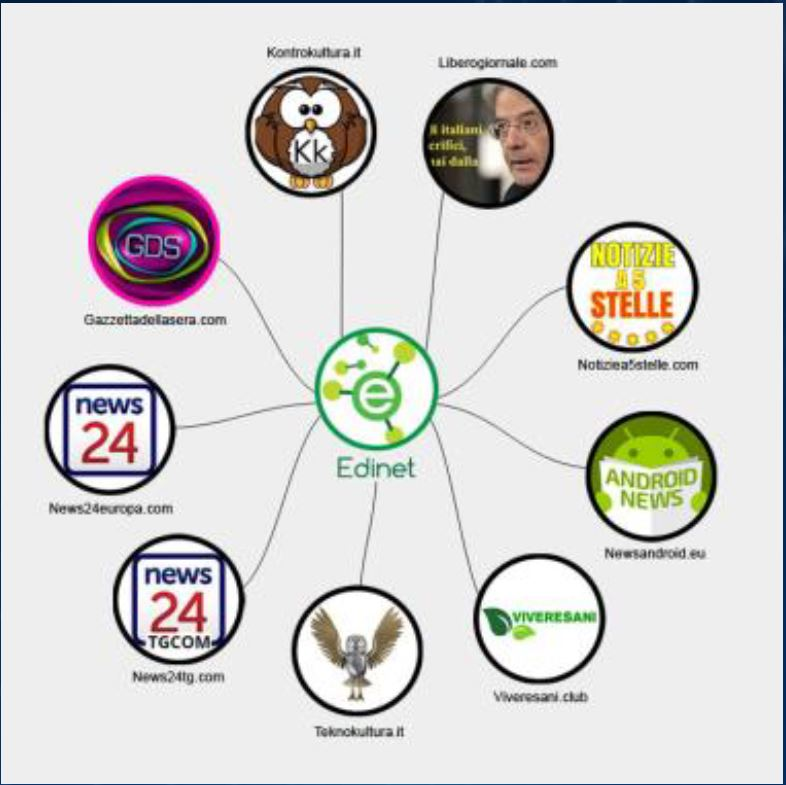
\includegraphics[width=0.5\textwidth]{images/10_lez_fig_01.jpg}
\end{figure}


Anche attraverso questo sistema è possibile moltiplicare la diffusione dell'informazione che viene diffusa. 

\subsection{Analfabetismo}
Un altro tema importante che gioca un ruolo fondamentale è l'analfabetismo. Parliamo di analfabetismo funzionale e di analfabetismo digitale. 
L'analfabetismo digitale normalmente caratterizza persone di una generazione non nata nel mondo digitale. Spesso le persone nate con le informazioni tradizionali non sanno gestire in modo completo e corretto lo strumento e si trovano in difficoltà quando si tratta di utilizzare gli strumenti che sono in continua evoluzione. 
Analfabetismo funzionale è quello che generalmente caratterizza i più giovani nativi digitali ma che non hanno acquisito una formazione sui contenuti e sulle possibilità di comprendere i contenuti tale da consettirgli di valutare l'attendibilità delle fonti e la correttezza delle informazioni.
Nell'autunno del 2016 l'Università di Stanford ha pubblicato uno studio dedicato proprio alla comprensione di come i giovani fra i 13-14 anni e 25 anni valutino la fonte delle informazioni e ne è emerso una grande incapacità di distinguere fra una fonte attendibile e una fonte inattendibile. 
Il ruolo nella diffusione sul web delle varie fonti è invece uguale. Non è detto che una fonte più attendibile o più seria abbia una capacità di diffusione delle informazioni maggiore di una fonte meno seria e meno attendibile. 
%20:05
\subsubsection{Facilità di pubblicazione}
Altro tema fondamentale pregio e difficoltà del web è la facilità con la quale si può arrivare a pubblicare qualsiasi tipo di commento. Qualunque utente sul web può generare contenuti informativi divulgandoli autoreferenziandosi. 
La grandissima differenza tra il web e i media tradizionali è proprio questa. Con i media tradizionali c'è un controllo, una verifica preliminare sull'informazione e soprattutto sull'autore dell'informazione per cui non tutto arriva a disposizione del pubblico. Basti pensare ad esempio ai giornali. Sui giornali scrivono i giornalisti professionisti, il pubblico può interagire, può commentare ma in un spazio ben preciso e ben dedicato che è quello delle lettere al giornale. 
Lo stesso discorso vale per la televisione. Il pubblico può interloquire, può partecipare come pubblico non come autore di nuovi contenuti. 
Nel web invece chiunque può aprire un blog, può pubblicare il proprio commento e può interagire con l'intero pubblico della rete.
Questo porta anche a delle conseguenze paradossali, ad esempio si trovano situazioni nelle quali il cittadino comune dibatte con l'esperto in una determinata materia pretendendo magari di spiegare come funzionano le cose. Qui mi piace citare una frase una dichiarazione di Piero Angela nel corso di un'intervista rilasciata nel febbraio-marzo del 2018 nella quale Piero Angela dice che la velocità della luce non si determina per alzata di mano. 
Occorre, nella possibilità di comunicare e dire la propria opinione,  trovare gli strumenti per distinguere fra un'opinione e una presa di posizione e un'affermazione di un esperto basata su ricerche, su fatti, su approfondimenti che non sono necessariamente del cittadino comune che si occupa magari di qualcos'altro. 

\subsubsection{Anonimato}
Altro tema importante è quello dell'anonimato. Sul web mediamente gli autori possono rimanere anonimi in primo luogo perché non c'è generalmente alcun obbligo né alcuna possibilità di controllo sulla effettiva identità di colui che apre un profilo, un account o che pubblica un commento. 
L'anonimato ha delle caratteristiche positive. Ci sono degli studi dell'UNESCO che chiariscono come la protezione dell'anonimato sia importante per le fonti giornalistiche in determinati contesti nei quali parlare liberamente è difficile. 
È anche vero che in alcune situazioni invece l'anonimato consente ai cosiddetti leoni da tastiera di diffondere informazioni di fare commenti, di denigrare il prossimo proprio con l'idea di non essere scoperti. 
Si dice anche che l'anonimato sul web è comunque una chimera perché spesso è possibile che la polizia postale, le autorità che fanno delle indagini, che hanno degli obblighi da adempiere rispetto a determinati contenuti che costituiscono un illecito possano rintracciare la persona.
Il fatto che sia possibile un anonimato porta anche ad una difficoltà di individuare se vi sono dei legami tra il sito informativo, tra l'informazione che viene distribuita e gruppi di potere. In altri termini, i legami fra un'informazione, fra i siti e determinati gruppi di potere può essere difficilmente riconoscibile con conseguente difficoltà quindi di comprendere quale sia l'effettiva fonte dell'informazione.
Ancora è possibile concentrare le fonti informative senza che questo sia immediatamente evidente. 
\subsubsection{Automazione}
\begin{itemize}
    \item I like e i profili sul web possono essere falsi. I profili possono essere creati da un unico soggetto o da più soggetti collegati ed essere replicati in maniera indiscriminata e incontrollabile. Anche i like su determinate immagini, notizie e post possono essere in realtà frutto di un'attività informatica di aumento di like con la conseguente ridistribuzione e ridiffusione sul web perché un contenuto che ha molti like viene indicizzato meglio, viene rivisto con più piacere perché anche l'utente che va a visualizzare le informazioni quando si rende conto che l'informazione ha un numero di visualizzazioni molto elevato, è invitato e aiutato ad andare ad aprire quell'informazione e a verificarla. In più, un numero di like molto importante contribuisce a creare una patente di attendibilità della notizia che viene diffusa.
    \item L'automazione consente anche un'aggregazione incontrollata e non trasparente fra informazioni diverse. È il fenomeno dell'indicizzazione delle informazioni che non è conosciuta né conoscibile da parte del grande pubblico.
    \item L'automazione consente una memoria locale delle ricerche precedentemente fatte. In altri termini, un utente che si pone davanti al web, quando cerca una determinata informazione, avrà facilmente restituite informazioni molto simili dello stesso tipo anche quando ritiene di fare una ricerca completamente nuova.
    \item L'automazione consente infatti di profilare le ricerche che sono state fatte dall'utente, consente di tenerne memoria e quindi in questo maniera consente di presentare all'utente che fa le sue ricerche delle informazioni molto simili, molto collegate, consente di restituirgli informazioni che il motore di ricerca o la piattaforma, o comunque il sistema, riconosce come informazioni che potrebbero essere gradite a chi fa la ricerca.



\end{itemize}

\subsubsection{Quali sono i rischi?}
\begin{itemize}
    \item un rischio è quello della manipolazione dell'informazione, quindi portare all'attenzione del pubblico un'informazione che è stata predigerita, precontrollata, premasticata in una maniera tale che un grande numero di persone continuerà ad essere convinta della verità di questa informazione.
    \item una delle preoccupazioni principali rispetto alla diffusione delle fake news è che queste possano essere un attentato ai processi politici e democratici. Nell'autunno del 2016, in occasione delle elezioni del presidente Trump negli Stati Uniti, si è cominciato a parlare dei rischi e della possibilità che le elezioni fossero state in qualche modo pilotate e controllate grazie alla diffusione di informazioni false sul web. All'epoca, autunno 2016, in inizio 2017, Facebook negò un suo possibile coinvolgimento, anche involontario, in un'operazione di questo tipo, è invece emerso nei primi mesi del 2018 che la società Cambridge Analytica avrebbe consentito avrebbe consentito la creazione di profili falsi su Facebook, i quali, a quanto sembrerebbe, effettivamente hanno contribuito alla divulgazione di informazioni che avrebbero aiutato l'elezione del presidente Trump.
    \item  La preoccupazione è al momento enorme, tanto che l'allarme sociale è tale che negli ultimi mesi del 2017 sono state adottate una serie di iniziative in ambito internazionale e presso diversi paesi, iniziative sia di studio, sia  di carattere normativo, che manifestano come ci sia una grande preoccupazione.
\end{itemize}

\textit{C'è un breve filmato in cu si fa vedere che se informazini sono verificate ci sono molte meno reazioni, è un episodio legato ai mussulmani.}
La diffusione di una informazione senza verifica dei fatti porta a una diffusione maggiore dell'odio. 
\begin{figure}[h]
    \centering
    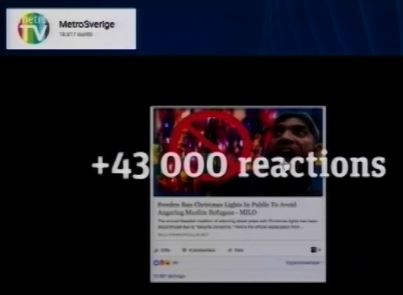
\includegraphics[width=0.5\textwidth]{images/10_lez_fig_02}
\end{figure}
Questo è realmente accaduto. Fact checking e non fact checking. 

\subsubsection{le dimensioni del fenomeno delle fake news}
Altro tema importante sono le dimensioni del fenomeno. Il fenomeno delle fake news ha due diverse dimensioni.
C'è un aspetto pubblico. L'interesse collettivo ad avere un'informazione corretta. La collettività nel suo insieme ha interesse a un'informazione corretta. Questo interesse della collettività si contrappone in qualche modo o comunque è un'altra faccia della medaglia dell'informazione perché dall'altro lato nelle società occidentali ognuno ha diritto di esprimersi liberamente e quindi di dire la propria versione. 
Per cui abbiamo un primo tema che è quello dell'interesse a informare da un lato dell'interesse a essere informati dall'altro. Nell'interesse a essere informati c'è l'importanza di un'informazione corretta. 
La pubblicazione di una notizia, di un'informazione può avere come contraltare quello di andare a toccare gli interessi di una singola persona. Quindi la seconda dimensione dell'informazione e della diffusione dell'informazione è l'interesse privato del singolo alla tutela della propria reputazione, alla tutela della propria identità, al diritto all'oblio di cui molto si parla e di cui avremo l'occasione di parlare meglio in una delle prossime lezioni. 
Il diritto pubblico ad avere determinate informazioni può essere in contrasto con l'interesse del singolo a veder cancellate quelle informazioni. La valutazione sul compromesso da adottare sulla prevalenza dell'uno o dell'altro è una valutazione che dovrà essere fatta caso per caso. 

\subsubsection{quali sono i possibili rimedi?}
Quali sono i possibili rimedi rispetto alla diffusione delle fake news? Ci sono tre orientamenti nel mondo occidentale su quali siano gli strumenti di contrasto rispetto alla diffusione delle fake news.
\begin{itemize}
    \item Un primo rimedio che lascia al lettore la valutazione è un approccio sostanzialmente liberista si dice è il lettore che deve essere formato e informato e migliorando le proprie competenze sarà in grado di individuare, di selezionare le informazioni corrette da quelle non corrette quindi è importante che sia il lettore a farsi una propria idea. 
    \item Un secondo orientamento propone che siano i fornitori di servizi internet a fare un'attività di verifica sulle notizie diffuse e di eventuale eliminazione delle notizie false. Sulla scorta di questo tipo di impostazione nel dicembre del 2017 Facebook ha proposto l'introduzione di un pulsante antibufala. Si tratterebbe di una sorta di bottone rosso che consente al pubblico, agli utenti di segnalare se un contenuto che è stato pubblicato è un contenuto discutibile, non reale.Dopodiché nel momento in cui c'è un gran numero di segnalazioni Facebook dovrebbe fare una verifica con dei fact checkers, cioè con delle organizzazioni riconosciute, accreditate di verifica dei fatti e poi eliminare l'informazione se è falsa o comunque segnalare che si tratta di un'informazione falsa. Questo tipo di soluzione presenta delle difficoltà perché si lascia sostanzialmente nelle mani di soggetti privati, di multinazionali che hanno come principale obiettivo il profitto, la valutazione su ciò che è vero e ciò che non è vero.
    \item La terza possibilità di intervento prevede l'intervento dei governi. I singoli governi o meglio ancora gli organismi internazionali dovrebbero prevedere un obbligo di verifica, segnalazione e rimozione con una valutazione però fatta da organismi di carattere internazionale e con la previsione di sanzioni a carico di coloro che pubblicano le fake news o che le lasciano in linea nel momento in cui sanno che si tratta di notizie false. Rispetto a questo tipo di soluzione le perplessità sono legate alla paura che da questo possa derivarne una forma di censura rispetto all'informazione pubblicata. 
\end{itemize} 

Non c'è quindi una presa di posizioni unica su quale sia il modo di risolvere le questioni.

Semplice domanda: perché le fake news diffuse sul web sono diverse da quelle diffuse sui media tradizionali? Cosa sono le fake news? 






\chapter{Fake news - seconda parte}

\section{Fake news - seconda parte}

Vi ricordo quello che abbiamo detto nella scorsa lezione. Le fake news sono delle notizie false che sono diffuse massivamente su internet e che possono ingannare, ingenerare delle false convinzioni negli utenti. Il problema delle fake news ha assunto delle dimensioni tali che nell'anno 2017 e anche nel 2018 due importanti enti in ambito europeo hanno deciso di assumere delle posizioni. 

Gli argomenti di oggi:

\begin{itemize}
    \item L'assemblea parlamentare del Consiglio d'Europa, il provvedimento che ha assunto
    \item commissione dell'Unione Europea High Level European Group (HLEG) on Fake News and Online Disinformation che è stato proposto dalla Commissione Europea e che ha elaborato un rapporto.
\end{itemize}

\subsection{L'assemblea parlamentare del Consiglio d'Europa}
Partiamo dal primo argomento, l'assemblea parlamentare del Consiglio d'Europa.
All'inizio del 2017 è stato elaborato un rapporto chiamato Media Online e Giornalismo, sfide e responsabilità. Si tratta della risoluzione numero 2143 del 2017 che è stata pubblicata il 2 febbraio del 2017. 
Di che cosa parla questa risoluzione? 
Parla della prevenzione e della diffusione di notizie false sul web. 

\begin{figure}[ht]
\centering
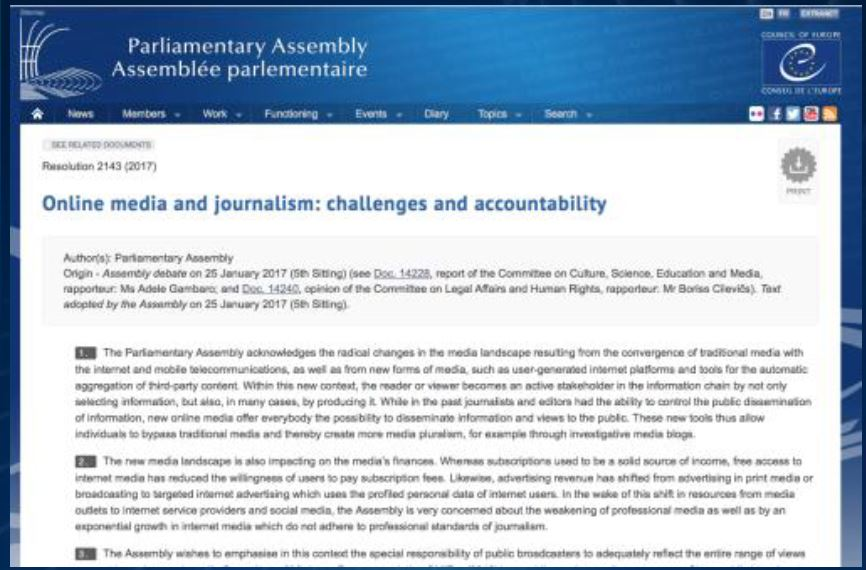
\includegraphics[width=0.8\textwidth]{images/11_lez_fig_01.jpg}
\caption{Pagina ufficiale sul sito con la pubblicazione del testo della risoluzione.}
\label{fig:11_lez_fig_01}
\end{figure}


Nella Figura \ref{fig:11_lez_fig_01} la pagina ufficiale sul sito con la pubblicazione del testo della risoluzione. Non potete leggere perché è soltanto un'immagine, ma potete vedere qual è il sito a cui fare riferimento e dove potete trovare questa risoluzione. \par
Come detto, la risoluzione si chiama Online Media and Journalism Challenges and Uncountability. Sono delle indicazioni di massima di quelle che sono le problematiche legate alla disinformazione online e degli spunti di riflessione e dei suggerimenti agli Stati membri su come è possibile intervenire per cercare di prevenire la diffusione della disinformazione online. \par
Da ricordarsi quando si parla di questo argomento che il web è uno strumento, un ambiente che offre un'infinità di possibilità. \par
Consente una partecipazione attiva del lettore. Il lettore può cercare quelle che sono le informazioni che lo interessano, ma può anche selezionare la produzione delle informazioni in maniera totalmente autonoma. Non solo, il web consente, ha consentito e continua a consentire sempre di più con lo sviluppo della tecnologia ad una informazione non professionale di farsi sentire e quindi la differenza rispetto al passato è enorme. \par
In passato l'informazione considerata tale, il giornalismo considerato tale, era soltanto un'attività di carattere professionale. Questo vuol dire che soltanto persone con una preparazione rispetto alla pubblicazione delle notizie avevano la possibilità concreta di far sentire la loro voce, di raccontare le loro opinioni, di esprimere, di raccontare la vita, il mondo, così come lo vedevano. \par
Con il web invece la possibilità di pubblicare informazioni non è più limitata agli organi tradizionali di informazione professionale, ma è aperta a chiunque. Chiunque con poco, con pochi strumenti, è in grado di pubblicare ciò che ritiene più importante o più opportuno. \par
È anche vero che il web permette di pubblicare informazioni a chiunque, permette anche di conoscere, di prestare attenzione a violazioni di diritti umani che possono essere rilevate in tutto il mondo a cui i media tradizionali a volte prestano scarza attenzione. \par
In questo senso il web è uno strumento formidabile per la diffusione di informazione, maggiore di quello che possono dare gli organi tradizionali. Questo modo di relazionarsi permette anche una mobilitazione di quello che è il cosiddetto popolo del web; le notizie che fanno presa sull'opinione pubblica possono portare a una mobilitazione molto forte di grandi masse di persone anche se non sempre sono basate su fatti reali o su informazioni obiettive. \par
E' capitato, e qui torniamo al tema delle fake news, della disinformazione, delle notizie false, sono capitati spesso episodi nei quali alcune notizie di grande effetto, generalmente corredate da fotografie o da video e da appelli a tutto il mondo tutto vengano ritenute oro colato e questo porta a grandi campagne di opinione, grande libertà di coinvolgere l'opinione pubblica ma anche grande rischio di coinvolgerla su informazioni che in realtà non sono fondate. 

\subsection{Le criticità del web}
Il web ha comunque delle grandi criticità, innanzitutto il tema del finanziamento dei mezzi di informazione. 
Con l'abitudine ad avere a disposizione notizie senza alcun limite, il popolo del web e gli utenti hanno una minore propensione ad abbonarsi agli organi di informazione. Questo però ha una contropartita, la ricerca, la pubblicazione, la selezione di notizie serie, il lavoro del giornalista e il lavoro del professionista è un lavoro appunto che richiede dei finanziamenti, l'organizzazione di un giornale, l'organizzazione di un canale media richiede dei finanziamenti, i giornali tradizionali, i media tradizionali sono stati spesso in parte finanziati dagli Stati ma anche finanziati dagli acquisti.\par
La minor propensione degli utenti ad abbonarsi ai canali di informazione crea un problema di tipo economico di cui bisogna tener conto. \par
Quindi spesso come è possibile finanziare l'informazione sul web? Attraverso la pubblicità e come avviene questo tipo di finanziamento, quali soggetti sono disposti a finanziare siti o blog e quant'altro? 
\subsubsection{Pubblicità e profilazione}
La valutazione sulla importanza di pubblicare una certa pubblicità sul sito dipende dai click, quanti più click un sito riceve, tanto più sarà facile che chi vuole fare pubblicità sia disposto a finanziare quel soggetto. 
Che cosa comporta però il rapporto fra visualizzazione di un sito e pubblicità? Che speso il click fatto sulla pubblicità viene utilizzato per profilare l'utente e si crea un rapporto incestuoso tra la profilazione e l'attività commerciale connessa alla pubblicità. 
%08:25
\subsubsection{Disinformazione e manipolazione sul web}
Possono essere messe in piedi delle campagne che sono realmente dirette a forviare l'opinione pubblica con informazioni false o anche con campagne d'odio. \par 
Abbiamo visto negli anni più recenti il modo in cui sono state impostate due importanti campagne elettorali nel mondo. Trump negli Stati Uniti e Macron in Francia. \par
In entrambi i casi si è fatto un ampio ricorso alle informazioni non tradizionali, a una diffusione di informazioni al di fuori dei canali ufficiali di informazione con strumenti come i social media, con strumenti di messaggistica istantanea, con Twitter. \par
Nel corso della campagna elettorale, più attori hanno diffuso notizie, magari semplicemente commenti, gossip su entrambi i candidati in modo diverso a seconda della campagna elettorale che è capitata. In entrambi i casi l'opinione pubblica è stata scossa e il timore è stato quello che l'opinione pubblica potesse essere distorta, che l'attenzione e la convinzione di tipo politico potesse avere un impatto importante sulla base di questi gossip e messaggi che erano spesso non veri. \par
\subsubsection{obiettivo del Consiglio d'Europa - Contrasto alle fake news}
Alla luce di tutta questa situazione l'obiettivo del Consiglio d'Europa è quello di trovare una maniera di contrastare le fake news perché:
\begin{itemize}
    \item creano allarme sociale
    \item permettono una manipolazione dell'opinione pubblica che può essere pericolosa, che può portare a direzionarla, a portarla verso degli obiettivi non trasparenti.
    \item permette di fare delle campagne d'odio nei confronti di singole persone o di gruppi sociali che possono destabilizzare anche gli Stati
    \item Perché una gestione delle fake news strutturata da parte di chi ha degli obiettivi magari non dichiarati può portare a contrastare quello che è il corretto processo democratico
\end{itemize}

L'informazione professionale secondo il Consiglio d'Europa ha un ruolo determinante come cane da guardia a tutela della imparzialità e della correttezza dell'opinione pubblica. Alla fine delle sue valutazioni quindi il Consiglio d'Europa fa una serie di raccomandazioni a più soggetti, agli Stati membri innanzitutto. 
\begin{itemize}
    \item L'invito è quello a stimolare un dibattito sulle norme possibili da adottare e su dei meccanismi di imprevenzione rispetto alla diffusione della disinformazione online.
    \item a individuare come tracciare gli utenti che violano la legge. E questo tema della tracciabilità è un tema particolarmente delicato. Il tracciamento degli utenti da un lato ha una grande utilità rispetto alla prevenzione o alla repressione di violazioni gravi di legge, dall'altro ingenera il timore che possa esserci un controllo sugli utenti che porterebbe a quella che è la temuta situazione del controllo a distanza. Ricorderete un importante romanzo di Orwell degli anni 80 nel quale si prefigurava proprio un controllo massivo della popolazione attraverso tecnologie informatiche.
    \item Dare un sostegno ai media tradizionali perché anche questi si adeguino agli standards che vengono oggi utilizzati online e facciano attenzione ai contenuti generati dagli utenti in maniera da tenerne conto, raccogliere quello che di buono viene e possano dialogare con gli utenti in maniera da mantenere desta l'attenzione, senza abbassare il livello di guardia rispetto alla correttezza delle informazioni.
    \item considerato questo rapporto fra l'informazione professionale e gli utenti, è importante garantire agli utenti un diritto di replica laddove vi sia da parte dell'informazione professionale un errore. E' anche un obbligo per l'informazione professionale di consentire all'utente la rettifica laddove ci sia appunto una falsa informazione.
    \item formazione rispetto al significato dell'informazione e della corretta informazione che deve partire dalla scuola e che poi deve portare anche a formare i professionisti in maniera adeguata e corretta anche sulle tecnologie attuali, anche sulle modalità di gestione dell'informazione online.
    \item di elaborare dei codici di condotta che possano essere esaminati in collaborazione con i media online e con gli internet service provider, soggetti che sono al di fuori del circuito informativo della raccolta e pubblicazione delle notizie, ma che hanno un ruolo enorme nella diffusione delle notizie e nel tenerle in piedi per lungo tempo.
    \item I proprietari dei siti devono in qualche modo essere responsabilizzati anche rispetto ai contenuti postati da terzi. La regola che fino adesso è stata la regola dominante nel web, è che l'internet service provider che non collaborando alla realizzazione dei contenuti non ha una responsabilità propria per quello che è il contenuto postato. È un po' poco perché il provider è quello che consente all'utente di farsi sentire e quindi in qualche maniera una forma di attenzione, non diciamo controllo, rispetto a quello che viene pubblicato e al fatto che non debba essere in contrasto con i diritti altrui, deve essere mantenuta anche da parte dei provider. 
\end{itemize}


%12:45
\subsubsection{Raccomandazioni per la Federazione Europea dei Giornalisti}
Vi sono nel rapporto anche delle raccomandazioni per la Federazione Europea dei Giornalisti. 

\begin{itemize}
    \item I giornalisti devono fare attenzione ad applicare anche al mondo internet i principi collaudati che sono applicati ai sistemi editoriali e i principi di deontologia.
    \item La pubblicità anche per l'informazione professionale è importante, va gestita e vanno individuati dei rimedi corretti per evitare che con l'uso della pubblicità si arrivi alla violazione di altri diritti come la profilazione. 
\end{itemize}

\subsubsection{Raccomandazioni per l'Associazione Europea dei Fornitori di Servizi Internet}

Il Consiglio d'Europa fa delle raccomandazioni all'Associazione Europea dei Fornitori di Servizi Internet che come abbiamo visto hanno un ruolo determinante nella diffusione dell'informazione. 

\begin{itemize}
    \item I fornitori di servizi internet dovrebbero dotarsi di un codice di deontologia 
    \item dovrebbero permettere agli utenti di segnalare le informazioni non corrette 
    \item dovrebbero anch'essi consentire una rettifica volontaria su richiesta di contenuti non corretti
    \item dovrebbero individuare da un punto di vista tecnico dei meccanismi di allerta e di segnalazione dei trolls.
\end{itemize}

Ecco qui quindi in sintesi quelle che sono le raccomandazioni del Consiglio d'Europa rispetto alla disinformazione online e quindi il più spunto di riflessione per voi. Che cosa raccomanda i governi il Consiglio d'Europa per contrastare le fake news? 

\section{High Level Group on Fake News and Online Disinformation}
La Commissione Europea e il High Level Group on Fake News and Online Disinformation. Cos'è l'High Level Group sulle fake news e disinformazione online? 
\begin{itemize}
    \item 
\end{itemize}

A dicembre 2017 la Commissione Europea ha lanciato l'istituzione del gruppo di lavoro sulle fake news e la disinformazione online.
A gennaio 2018 si è installato, ha cominciato i lavori e a marzo 2018 ha pubblicato il suo rapporto. 
Il tema sono le fake news e in particolare l'individuazione, la definizione, il contrasto alla loro diffusione.

\begin{figure}[h]
\centering
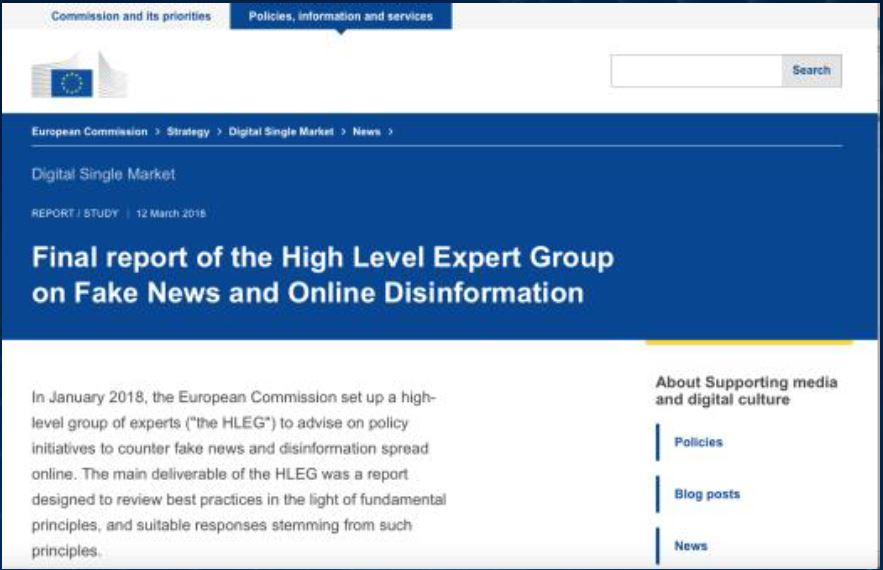
\includegraphics[width=0.9\textwidth]{images/11_lez_fig_02.jpg}
\label{fig: High Level European Group}
\caption{Final Report of the High Level European Group on Fake News and Online Disinformation}
\end{figure}

In Figura \ref{fig: High Level European Group} è per darvi un'idea di quello che è il sito sul quale la Commissione Europea ha pubblicato i lavori della Commissione e soprattutto il rapporto finale del gruppo di esperti sulle fake news e la disinformazione online. \par
I presupposti da cui partono gli esperti per l'elaborazione del loro lavoro è:
\begin{itemize}
    \item il fatto che c'è una stretta interconnessione tra la disinformazione e lo sviluppo dei media digitali
    \item sul web interagiscono una serie di attori diversi, pubblici e privati, commerciali, i media, i cittadini. Ci sono attori individuali e ci sono gruppi di utenti che operano.
\end{itemize}

Questi due elementi sono i presupposti dai quali è partito il gruppo di lavoro per elaborare il suo studio. La Commissione, il gruppo di lavoro, è consapevole che la disinformazione è un fenomeno che va ben oltre il termine fake news.\par
Con questo intende dire che le fake news, secondo il gruppo di esperti, sono solo una fetta della disinformazione online ed è la fetta della quale il gruppo si vuole occupare.\par
Il termine fake news tra il 2017 e il 2018 è diventato talmente importante che per il Collins Dictionary è stato il termine dell'anno 2017 a causa del numero di volte in cui è stato utilizzato sul web. \par
Secondo il gruppo di lavoro della Commissione europea però questo termine è stato utilizzato spesso in modo mistificatorio per indicare anche quello che è semplicemente sgradevole. Non tutto ciò che viene chiamato fake news è veramente fake news. \par 
Che cosa include il gruppo di lavoro nella sua definizione? \par
Innanzitutto fake è ogni informazione falsa, inaccurata o ingannevole che è stata indicata, presentata o promossa per provocare preoccupazione o per ottenere profitto, in ogni caso con intenzionalità. \par
Non è inclusa nella definizione del gruppo di lavoro la creazione e la disseminazione di contenuti illegali, quindi fake nella definizione del gruppo di lavoro non è illegale e come contenuti illegali intendiamo contenuti di carattere diffamatorio, hate speech, incitamento alla violenza. Questo tipo di contenuti illegali sono già regolamentati all'interno dell'Unione europea e degli Stati membri e questa è la ragione per la quale la Commissione ha ritenuto di non prenderli in considerazione.\par
Non rientra nelle fake news la distorsione dei fatti, deliberata ma non ingannevole, ad esempio individuabile nella satira o individuabile nella parodia.\par
Una volta individuati i limiti e i parametri, il gruppo di lavoro ha cercato di individuare i fondamenti per il contrasto alle fake news.
%22:17
\subsection{Fondamenti per il contrasto alle fake news}

Il gruppo di lavoro è consapevole che non esistono soluzioni facili per risolvere il problema, ogni soluzione è comunque complessa e richiede un approfondimento da vari punti di vista. \par

\begin{itemize}
    \item uno degli elementi principali di cui si è tenuto conto è che nell'elaborare delle forme di contrasto e di prevenzione delle fake news, è fondamentale tutelare sempre la libertà di espressione, che è uno dei principi fondanti dell'ordine democratico dei Paesi occidentali
    \item è necessaria una collaborazione di tutti gli stakeholders
    \item è anche necessario un monitoraggio costante dell'evoluzione di ciò che accade sul web
\end{itemize}

Ciò detto, sono stati individuati cinque pilastri. 

\begin{itemize}
    \item Inanzitutto la trasparenza delle notizie, come nascono, come vengono pubblicate
    \item l'alfabetizzazione, che deve essere alfabetizzazione digitale per le generazioni che non sono native digitali, e alfabetizzazione di contenuti, di concetto delle generazioni più giovani
    \item responsabilizzazione di utenti e giornalisti. Da una parte e dall'altra, proprio per il fatto che, come abbiamo visto, sia utenti che giornalisti possono inserire contenuti, è importante che tutti capiscano che devono assumersi delle responsabilità rispetto all'informazione online
    \item la sostenibilità e la diversità dei media all'interno dell'Unione Europea. Nel mondo del 2018 e nel futuro, i media online e offline convivono, e devono continuare a convivere più tipi di media, perché la pluralità è uno degli strumenti essenziali per una informazione libera e corretta. Entrambi questi strumenti, online e offline, devono essere sostenibili da tutti i punti di vista, compreso quello economico
    \item la ricerca. Occorre fare una ricerca continua di quello che è l'impatto delle notizie, di quello che è l'impatto dei media e di quelle che sono le risposte rispetto agli interventi adottati
\end{itemize}

\subsubsection{Raccomandazioni del gruppo di lavoro}
Dopo aver elaborato i cinque pilastri, il gruppo di lavoro ha individuato una serie di raccomandazioni a diversi soggetti. 
Inanzitutto alla la Commissione Europea.
\par
A breve termine: 
\begin{itemize}
    \item La prima raccomandazione, a breve termine, è quella di elaborare dei codici di condotta per tutti gli stakeholders che sono coinvolti
    \item di mettere in piedi un centro di ricerca europeo per affrontare il tema
    \item di promuovere il supporto per dei progetti innovativi che si occupino di questi argomenti
\end{itemize}

A medio-lungo termine:

\begin{itemize}
    \item promuovere delle attività, delle iniziative per l'alfabetizzazione e delle best practices
    \item Promuovere e istituire un safer internet center
    \item individuare e dare agli Stati membri una guida per l'adozione di misure fiscali che consentano la sostenibilità di iniziative valide e corrette per la promozione dell'informazione corretta

\end{itemize}

\subsubsection{Raccomandazioni agli Stati membri}
Il gruppo di lavoro dà delle raccomandazioni agli Stati membri.\par

A breve termine:

\begin{itemize}
    \item individuare dei fondi e strumenti per la ricerca
\end{itemize}

A medio-lungo termine:
\begin{itemize}
    \item promuovere l'alfabetizzazione e la formazione
    \item rafforzamento dell'indipendenza dei media rispetto a forme di pressione di qualunque genere
    \item Sostenibilità finanziaria dei media attraverso forme fiscali, adeguate e corrette, in modo da rendere sostenibile un'informazione corretta e l'innovazione nell'informazione
\end{itemize}


\subsubsection{Raccomandazioni alla società civile}
Da ultimo, la Commissione dà delle raccomandazioni alla società civile.\par
Le raccomandazioni sono  a medio e lungo termine. 

\begin{itemize}
    \item La società civile dovrebbe individuare delle forme di collaborazione alla ricerca anche attraverso l'istituzione di community di cittadini che collaborino
    \item dovrebbero essere elaborate delle piattaforme, dei tools di condivisione degli standard informativi, tali che permettano agli utenti di lavorare in maniera simile a come lavorano coloro che hanno  le piattaforme
    \item dovrebbe stimolare la nascita di New Media pretendendo un'informazione di qualità e operando perché vi sia un corretto fact checking e perché vi sia un approccio etico all'informazione
    
\end{itemize}


Riepilogando, il gruppo di lavoro della Commissione europea, dopo aver individuato il significato di fake news per quello che è l'obiettivo che aveva il gruppo di lavoro, ha dato dei pilastri sui quali fare riferimento e che hanno guidato l'elaborazione del rapporto. Ha poi individuato tutta una serie di azioni da mettere in piedi da parte dei diversi stakeholders interessati al tema, alla Commissione europea, agli stati membri, ai media e alla società civile.\par 
Lo spunto di riflessione per questo argomento. Quali sono i cinque pilastri proposti da Heigh Level Gruop on fake news? \par
Riepiloghiamo gli spunti di riflessione della lezione che abbiamo appena ascoltato:

\begin{itemize}
    \item Cosa raccomanda ai governi il Consiglio d'Europa per contrastare le fake news?
    \item Quali sono i cinque pilastri proposti da Heigh Level Gruop on fake news?
\end{itemize}

Con questa lezione abbiamo concluso l'argomento delle fake news. 
Come ricorderete, questo argomento è stato trattato in due lezioni e questo vi fa capire quanto il tema sia un tema importante. Probabilmente, anche mentre state ascoltando questa lezione, qualcosa è già cambiato. Basti dirvi che a seguito della pubblicazione del rapporto del gruppo di lavoro della Commissione europea, ci sono stati degli eventi importanti che hanno ancora una volta portato all'attenzione del pubblico il problema.\par 

Qual è la dimensione del problema? Proprio nella primavera del 2018, nel marzo-aprile 2018, è scompiato lo scandalo chiamato Cambridge Analytica. \par
Che cosa è successo? È successo che un dubbio che si era posto fin dalla campagna elettorale di Trump, si è iniziato a pensare che forse le fake news sono uno strumento che ha portato a un cambiamento delle decisioni.\par
Il dubbio era stato sollevato, Mark Zuckerberg aveva negato la possibilità di un convolgimento di Facebook rispetto a questo evento. A distanza di un anno e mezzo, invece, questo timore è stato confermato. A primavera, ad aprile del 2018 è emerso che attraverso la società Cambridge Analytica sono stati utilizzati dei profili su Facebook, sono stati violati e sono state diffuse delle informazioni finalizzate proprio a promuovere la posizione di Trump.\par 
Ne è nato uno scandalo enorme, Facebook ha perso moltissimo dal punto di vista economico in borsa e la società Cambridge Analytica è praticamente andata in default per questa ragione. Questo ha portato di nuovo all'attenzione dei governi l'importanza di questo tema. \par
Ancora siamo lontani dal trovare una soluzione, ma certamente va individuata una soluzione senza con questo in alcun modo limitare quello che è il diritto di informazione, la libertà di espressione che deve comunque sempre essere garantita a tutti i cittadini. 
\chapter{Lezione 12: La rivoluzione digitale nella pubblica amministrazione}

Il tema di questa lezione è la rivoluzione digitale nella pubblica amministrazione. 

Gli argomenti di oggi sono:
\begin{itemize}
    \item L'amministrazione digitale
    \item La documentazione digitale
\end{itemize}

\section{L'amministrazione digitale}

Iniziamo dal primo argomento, l'amministrazione digitale. 

Per amministrazione digitale si intende la digitalizzazione dell'amministrazione, processo disciplinato e incentivato dal \textbf{codice dell'amministrazione digitale}, di solito abbreviato in CAD, che è stato emanato con Decreto Regislativo 82/2005 e successivamente soggetto a numerose modifiche, alcune incisive; una modifica abbastanza importante nel 2010 e ulteriori modifiche nel 2011.

Per amministrazione digitale si intende l'applicazione delle tecnologie informatiche e telematiche all'attività amministrativa e a tutto ciò che supporta lo svolgimento dell'attività amministrativa e altresi al prodotto, diciamo al pervedimento \footnote{pervedimento: Arrivare, giungere, sia in senso generico sia (oggi più spesso) quando il luogo o punto d'arrivo rappresenta il termine di un viaggio lungo, di un percorso faticoso o che ha comunque richiesto il passaggio attraverso gradi successivi o il superamento di qualche difficoltà}, dell'attività amministrativa.

Si è parlato di una rivoluzione culturale nella pubblica amministrazione. 

Il modo in cui si raffigura e si pratica la pubblica amministrazione in Italia è tradizionalmente legata alla carta, ai timbri, al potere certificativo del pubblico ufficiale che appone una firma e un timbro, alla richiesta di documenti autentici, sottoscritti, firmati degli interessati, da chi avanza certe richieste o effettua certi adempimenti per la pubblica amministrazione, dalla richiesta per esempio di ricevere pagamenti di un certo tipo, in contanti o con bollettini postali e così via.

L'immagine tradizionale della pubblica amministrazione che si cerca faticosamente di superare in Italia  è quella di un pachiderma, di un macigno che ha procedure lente, farragginose, burocratiche, che comportano lo spostamento di carte polverose da un ufficio all'altro, che necessitano di firme su documenti stampati su carta, che attendono su scrivanie, eccetera eccetera.

È fatto anche di scarsa comunicazione sia con l'utenza, i cittadini, sia con le altre amministrazioni e così via.

Da alcuni decenni, in particolare a partire dalla legge 241 del 90 e poi anche per l'effetto di vari principi comunitari, si è cominciato a immaginare un ripensamento della cultura della pubblica amministrazione in Italia, non solo di singole strutture organizzative, ma della stessa cultura della pubblica amministrazione. Si è cercato di ripensare la cultura della pubblica amministrazione come un'attività statale dotata di imperio e di una certa posizione talvolta tacita, di supremazia nei confronti dei cittadini, quindi talvolta anche di scarso rispetto per le loro esigenze, da qui il prolungarsi abnorme, irragionevole, dei tempi di molte procedure amministrative, richieste dei cittadini, creando difficoltà.

Per esempio si pensi alle difficoltà che può avere un'attività commerciale nell'attendere il rilascio di tutte le licenze e autorizzazioni previste dalla legge.

Quindi si è cercato di immaginare una trasformazione culturale nella pubblica amministrazione da una visione statica della pubblica amministrazione quasi autoreferenziale e in una posizione di supremazia nei confronti dei privati ad una concezione sempre più di servizio della pubblica amministrazione.

L'amministrazione come servizio ai cittadini, l'amministrazione che al suo interno viene organizzata in maniera premiale in vista dei risultati.

Le burocrazie e gli uffici amministrativi devono agire sulla base dei risultati e perseguirli sulla base dei criteri, dei principi di economicità, efficacia, efficienza, trasparenza, pubblicità e legalità.

Questi sono i principi fondanti, i criteri base dell'attività amministrativa dalla fine del XX secolo in poi, quindi quantomeno dalla legge 241 del 90 in poi.

Legalità, il fatto che l'attività amministrativa deve svolgersi nell'ambito di una cornice di criteri, direttive e principi stabiliti dalla legge, altresì deve esserci una conformità tra i provvedimenti adottati dalla pubblica amministrazione e gli scopi e i presupposti indicati dalla legge, legalità, trasparenza e pubblicità, il fatto che il cittadino ha diritto di accedere e partecipare a vario titolo all'attività amministrativa, per esempio la legge sul procedimento amministrativo, appunto la già citata legge 241 del 90, che prevede che il cittadino abbia un diritto di accesso e di partecipazione, diritto per esempio di interlocuire, nell'ambito di procedimenti che lo riguardano, ha diritto a produrre documenti e così via, ha diritto che le sue istanze vengano tenute in considerazione nell'adozione del provvedimento finale.

Il cittadino ha diritto di partecipare ai procedimenti, diritto di accesso ai documenti che lo riguardano, diritto a consultare certi documenti e così via, quindi trasparenza, pubblicità, efficacia ed efficienza.
Per efficacia si intende l'esigenza che la pubblica amministrazione raggiunga i propri scopi in maniera concreta, quindi che la pubblica amministrazione raggiunga realmente gli scopi che si prefigge, gli scopi dell'azione amministrativa.

Per efficienza si intende l'esigenza che gli scopi perseguiti dall'autorità amministrativa siano perseguiti col minore dispendio possibile di risorse, quindi che siano usate le risorse umane e economiche effettivamente necessarie allo raggiungimento dello scopo, senza inutili sprechi di risorse.
%07:30
E' evidente che in questo processo di ripensamento culturale della pubblica amministrazione, ispirato i criteri di trasparenza, pubblicità, efficacia, efficienza e così via, si inserisse in maniera senz'altro inevitabile le più generali procedure e risorse rese disponibili dalle tecnologie della società dell'informazione. 

Quindi a un certo punto è sembrato inevitabile che tutte le esigenze che abbiamo annunciato, la pubblicità, la trasparenza, i diritti partecipativi dei cittadini nei confronti dell'attività amministrativa, l'efficacia, l'efficienza, eccetera, tutti queste esigenze potessero essere soddisfatte o raggiunte o comunque potessero trovare un valido sostegno nelle tecnologie dell'informazione, nella digitalizzazione e nella informatizzazione delle attività amministrative, delle procedure e anche degli atti dei documenti amministrativi.

Questo spiega appunto la rivoluzione culturale che molti si attendono, da un'amministrazione autoreferenziale in posizione di supremazia ad un'amministrazione di servizio e di risultato.
Questa è la rivoluzione più generale. All'interno di questa rivoluzione più generale c'è una seconda rivoluzione che è quella della informatizzazione della pubblica amministrazione, della trasformazione di gran parte delle attività amministrative in attività informatizzate e digitalizzate. 

Questo dovrebbe consentire il raggiungimento di vari obiettivi, l'abbattimento dei costi, una maggiore trasparenza, forse anche una maggiore considerazione per l'ambiente, nella misura in cui vi sia meno uso e meno spreco di carta. 

Vediamo come possiamo tradurre l'incrocio di queste due rivoluzioni in base ai principi indicati dal codice dell'amministrazione digitale.

Quali sono gli obiettivi, o alcuni degli obiettivi, previsti dal codice dell'amministrazione digitale? 

Una rivoluzione culturale nella PA: maggiore efficienza e trasparenza: ‘dialogo’ telematico tra PA e con i privati, con pieno valore legale; alfabetizzazione informatica dei dipendenti.

O meglio per una maggiore efficienza e trasparenza, promuovere il dialogo telematico tra pubbliche amministrazioni e tra la pubblica amministrazione e i privati, con pieno valore legale, promuovere l'alfabetizzazione informatica dei dipendenti. 
Iniziamo da questi. 
%10:45
\subsection{Promuovere maggiore efficienza e trasparenza}

E' evidente che il ricorso all'informatizzazione e anche alla telematica può incentivare questi processi. Per esempio tutte le pubbliche amministrazioni dovrebbero dotarsi di siti Internet che enunciano chiaramente per esempio la struttura dell'ufficio, i contatti, le persone a cui riferirsi, gli orari di ricevimento del pubblico, la modulistica, una sintesi delle procedure che svolgono, indichino le loro funzioni e così via.

In questo modo l'amministrazione diventa trasparente rispetto al cittadino, perché il cittadino sa a quali amministrazione rivolgersi, sa a chi rivolgersi all'interno dell'amministrazione, produce già da casa o dall'ufficio la modulistica rilevante, eccetera eccetera.

\subsection{Dialogo telematico tra pubbliche amministrazioni e tra pubbliche amministrazioni e privati}

Spesso le pubbliche amministrazioni non comunicano contro loro. Le pubbliche amministrazioni raccogono grande quantità di dati personali dei cittadini per i loro scopi istituzionali ma spesso però i cittadini sono obbligati a ripresentare le stesse informazioni o modulistiche che contengono le stesse informazioni a diverse amministrazioni per ottenere determinati tipi di provvedimenti che a loro interessano o per svolgere certi adempimenti. 

L'idea è che facendo dialogare e interagire le banche dati delle varie amministrazioni, con certi limiti per problemi di riservatezza dei dati, si possono realizzare risultati in termini di efficienza e efficacia dell'azione amministrativa anche in termini di risparmio di tempo per i cittadini. 

Inoltre il dialogo telematico tra la pubblica amministrazione e i privati è un vero e proprio diritto istituito dal codice dell'amministrazione digitale di dialogare in maniera telematica con la pubblica amministrazione. 

Che cosa vuol dire? La possibilità si scaricare documenti in formato elettronico, produrre documenti in formato elettronico, quindi attribuire un certo valore legale al documento formato in maniera elettronica e poi trasmetterli alla pubblica amministrazione con strumenti elettronici, per esempio con la posta elettronica. 
%13:30
Ovviamente questo presuppone una massiccia opera di alfabetizzazione informatica dei dipendenti della pubblica amministrazione con corsi di formazione, presuppone un cambiamento di cultura, cioè il progressivo abbandono della carta e la coscienza nei pubblici dipendenti che ciò è necessario. 

Il codice dell'amministrazione digitale è di fatto il primo intervento sistematico in materia. A partire dagli anni 90, si erano susseguiti interventi su settori diversi della pubblica amministrazione, in particolare erano provvedimenti non benissimo collegati tra loro, ma comunque adottati in tempi diversi sul documento informatico, sulla firma digitale, sulla trasmissione attraverso la posta elettronica dei documenti, sulla tenuta dei archivi e così via. 

Il codice dell'amministrazione digitale si prefigge di essere un intervento organico che ridisegna in maniera complessiva il sistema e la dimensione digitale informatizzata della pubblica amministrazione. 
%14:56
Probabilmente uno dei limiti del codice della pubblica amministrazione è una certa enfasi declamatoria, forse un eccessivo ottimismo, perché contiene soprattutto enunciazioni di principi che ad alcuni sono sembrati fumosi e la cui attuazione richiede sforzi e risorse coordinate e un impegno serio e costante. 

Si enunciano diritti come il diritto del cittadino al dialogo digitale con la pubblica amministrazione e così via. 

Se si vuole che questi principi diventino realtà sono necessari, innanzitutto numerosi atti normativi di dettaglio e soprattutto un cambiamento culturale nella pubblica amministrazione. 

Un elemento in tal senso è presente nelle successive modifiche del codice della amministrazione digitale, soprattutto  quelle del 2010 e 2011, in cui si cerca di introdurre un'ottica sanzionatoria premiale nei confronti delle pubbliche amministrazioni, sanzionatoria per un verso, premiale per l'altro, che progressivamente si dotano di questi strumenti e traducono la loro attività amministrativa in termini informatici e telematici. 

Allora l'oggetto della disciplina, del codice dell'amministrazione digitale, in generale è l'utilizzo delle tecnologie informatiche e telematiche nella pubblica amministrazione, tramite tutta quella serie di principi che abbiamo menzionato poc'anzi. 

Il sistema pubblico di connettività, vale a dire un'integrazione sempre maggiore e tendenzialmente globale di tutte le pubbliche amministrazioni centrali, periferiche, amministrazioni locali e così via, in un sistema pubblico di connettività, in una rete che integri e che faccia comunicare nella maniera più efficiente ma anche nella maniera più sicura possibile le pubbliche amministrazioni. 
%17:40
La sicurezza è un presupposto indispensabile per la circolazione dei dati vista la quantità di informazioni personali anche sensibili, come dati sulla salute che vengono resi da un dipendente pubblico va in aspettativa, o dati sulla salute richiesti quando si accede a certe prestazioni previdenziali e assistenziali e così via.

Il sistema pubblico di connettività che dovrebbe succedere a vari esperimenti già attuati da alcuni decenni, per esempio la Rupa, la rete unitaria della pubblica amministrazione e così via. 
Quindi un'unica rete, un sistema di connessione che riguarda tutte le pubbliche amministrazioni. 

\subsection{Il valore giuridico del documento informatico e delle firme elettroniche}

La pubblica amministrazione produce documenti che hanno un certo valore legale e spesso la pubblica amministrazione acquisisce o richiede l'acquisizione da parte dei privati di documenti che hanno un certo valore legale. Se la produzione o l'acquisizione di documenti da parte della pubblica amministrazione viene fatta sul supporto informatico è necessario stabilire le condizioni alle quali questa documentazione informatica ha valore legale e di ciò si occupa per l'appunto il codice dell'amministrazione digitale.

L'efficacia legale di questi documenti va oltre quello amministrativo ma è ovvio che era necessario trattare di questo tipo di profilo nell'ambito di una normativa generale sulla informatizzazione della pubblica amministrazione. 

Lo stesso vale per la posta elettronica certificata che è un altro degli argomenti che ricadono nell'ambito di disciplina del codice o delle normative che esso delega. 
Il codice richiede l'adozione di documenti attuativi, decreti ministeriali che contengono regole tecniche per esempio sulla produzione di documenti digitali, sulla posta elettronica certificata e così via; regole per la trasmissione elettronica avente valore legale di atti tra pubblica amministrazione e tra le pubbliche amministrazioni e i privati e questo viene fatto con la normativa inclusa in questo corpus sulla posta elettronica certificata.


\subsection{Finalità del codice dell'amministrazione digitale}

Iniziamo a valutare le finalità sia di medio che di lungo periodo del codice dell' amministrazione digitale. Lo Stato, le Regioni e le Autonomie Locali assicurano la disponibilità, la gestione, la trasmissione, la conservazione e la fruibilità dell'informazione in modalità digitale e si organizzano ed agiscono a tal fine, utilizzando con le modalità più appropriate, le tecnologie dell'informazione e della comunicazione.

Qui abbiamo alcuni spunti interessanti. Innanzitutto il fatto che venga istituito questo diritto del cittadino a fruire in maniera digitale e informatizzata dei servizi amministrativi. Ricevere prestazioni tramite supporto, per esempio comunicazioni da parte di uffici amministrativi, tramite email, tramite posta elettronica, inviare comunicazioni tramite email e quindi inviare documenti aventi valore legale, quindi formati sul supporto elettronico, anche questi inviarli tramite strumenti elettronici e telematici.

Più in generale la strutturazione dell'azione amministrativa con le opportunità rese possibili dalle tecnologie dell'informazione e delle telecomunicazioni. 

Il rinvio che viene fatto da questo corpo normativo alle tecnologie è ovviamente un rinvio mobile, vale a dire che le norme di principio contenute nel codice dell'amministrazione digitale non indicano in maniera precisa quali sono le tecnologie da utilizzare in quanto dovranno essere utilizzate le migliori o le più opportune tecnologie disponibili al momento e perché l'evoluzione tecnologica in sé che le consiglia, oppure perché, saranno previsti di volta in volta alcuni decreti ministeriali o decreti del Presidente del Consiglio dei Ministri per l'adozione di specifiche tecniche più opportune per certi fini. 
%23;27
La normativa di solito, per esempio i decreti ministeriali o decreti del Presidente del Consiglio e in certa misura anche il codice individuano criteri di base che devono essere eseguiti per la formazione di documenti e per trasmissioni di comunicazioni elettroniche;per esempio se sono soddisfatte queste regole di base, un certo documento prodotto avrà valore legale, efficacia probatoria, eccetera, eccetera. 

Il codice dell'amministrazione digitale si prefigge altresì obiettivi di lungo periodo. Sono poco più che declamazioni, ma probabilmente è possibile per esempio abbiano una utile funzione culturale anche queste proclamazioni nel codice. 
Promuovere iniziative per l'alfabetizzazione informatica dei cittadini, lotta al digital divide, il divario digitale che è ciò che separa i cittadini, i soggetti che non hanno familiarità e possibilità anche fisica, economica, materiale, di accesso alle risorse informatiche. 
Per fisica si intende, per esempio, la predisposizione di strumenti informatici o modalità di fruizione degli strumenti informatici da parte dei soggetti affetti a disabilità, anche di questo si occupa il codice dell'amministrazione digitale. 

È ovvio che se l'amministrazione e i cittadini viaggiasero a due velocità nettamente diverse dal punto di vista dell'informatizzazione, questo produrrebbe forme di esclusione da diritti di cittadinanza di molti cittadini. Se la pubblica amministrazione viaggiasse a livelli di informatizzazione tali che molti cittadini non riuscissero a dialogare con tali risorse informatiche digitali della pubblica amministrazione, si creerebbero forme di esclusione sociale, cioè l'impossibilità di molti cittadini di accedere ai servizi digitali e ai servizi informatici della pubblica amministrazione. Di conseguenza il complemento culturale della digitalizzazione e informatizzazione nella pubblica amministrazione è ovviamente l'alfabetizzazione digitale e l'alfabetizzazione informatica dei cittadini e questo è uno degli obiettivi di lungo periodo che si propone il codice. 

Ulteriore obiettivo è favorire l'uso delle nuove tecnologie per una maggiore partecipazione dei cittadini al processo democratico e facilitare l'esercizio dei diritti politici e civili, ed è ciò che si chiama e-democracy digitale.
%26:42
Quindi le tecnologie dell'informazione sfruttate dalla pubblica amministrazione in una prospettiva di lungo periodo dovrebbero essere finalizzate non solo alla fruizione di servizi amministrativi ma anche alla partecipazione dei cittadini al processo democratico, in che modo non è chiarissimo oggi, sono promesse per il futuro, è la facilitazione dell'esercizio dei diritti civili e politici. 

Per esempio si potrebbe prevedere una estensione o una implementazione del voto elettronico che potrebbe essere svolto anche a distanza, in presenza di certi presupposti, per facilitare l'esercizio del voto elettronico anche da parte di persone che sono fisicamente impossibilitate a recarsi nei seggi elettorali.
Queste sono però promesse per un futuro in cui contorni ancora non si scorgono. 

\subsection{Diritto all'uso delle tecnologie}

I cittadini e le imprese hanno diritto a richiedere ad ottenere l'uso delle tecnologie telematiche nelle comunicazioni con le pubbliche amministrazioni; si pone in capo ai cittadini e alle imprese la possibilità, a cui si dà la veste di diritto giuridico, anche se tuttora non è chiaro quali siano gli strumenti per sanzionare l'inottemperanza di questo diritto, affinché i loro rapporti con le pubbliche amministrazioni si svolgano tramite l'utilizzo di tecnologie informatiche e telematiche. 

Per esempio per le imprese lo stesso codice prevede l'istituzione di uno sportello unico per le imprese con il quale le imprese possono dialogare e interagire anche in maniera telematica. Oppure altri esempi, alcuni dei quali già vigenti, come la possibilità di accedere a certi servizi come ad esempio fare visure sui registri delle imprese, dentro le camere di commercio, visure catastrali, fare queste visure in maniera telematica, per esempio da uno studio notarile o da uno studio legale. Quindi interagire da parte di tutti i cittadini, da parte di imprese, da parte di particolari soggetti qualificati, interagire con le pubbliche amministrazioni con strumenti informatici e telematici. 

\subsection{Participazione al procedimento amministrativo informatico}

Il procedimento amministrativo è una procedura svolta da una pubblica amministrazione che si articola in vari passaggi che è preordinata che ha il fine di adottare un certo atto o provvedimento amministrativo. I cittadini che sono interessati all'adozione di quel procedimento amministrativo, perché per esempio quel provvedimento inciderà sulla loro sfera giuridica, hanno diritto a partecipare al procedimento amministrativo e questo è un diritto già stabilito in via generale dal 1990 con la legge 241; ma in base ai principi del codice dell'amministrazione digitale hanno diritto di partecipare a questo procedimento e di accedere agli atti prodotti o utilizzati nell'ambito di questo procedimento tramite l'uso delle tecnologie informatiche. 

Quindi, per esempio, richiedere  la comunicazione via posta elettronica di certi atti di un procedimento. Normalmente in fase pre-digitale l'accesso si esercitava recandosi personalmente presso l'amministrazione che detiene quei documenti. Questo richiedeva dispendio di tempo, una volta anche di denaro, se l'amministrazione si trova in una città diversa. Quindi accedere fisicamente a questi documenti ha un costo in termini di tempo e di denaro; l'utilizzo delle nuove tecnologie potrebbe tagliare significativamente questi costi. 

Ogni atto e documento può essere trasmesso alle amministrazioni pubbliche con l'uso delle tecnologie e dell'informazione se è formato ed inviato nel rispetto dell'evigenza normativa. Il diritto al dialogo digitale con la pubblica amministrazione che dicevamo prima. È chiaro che per questo sono necessari dei presupposti, vale a dire che il documento e anche la sua trasmissione vengono formati secondo certi presupposti, certe regole tecniche indicate di volta in volta dalla normativa rilevante. 

\subsection{Compiti della pubblica amministrazione}
Compiti della pubblica amministrazione nell'implementare i principi, i criteri direttivi stabiliti dal codice dell'amministrazione digitale. 

\begin{itemize}
    \item Realizzare gli obiettivi di efficienza, efficacia, economicità, trasparenza, semplificazione e partecipazione. In buona misura abbiamo già visto cosa significhi ciascuno di questi obiettivi, sono i principi cardine della nuova pubblica amministrazione a partire dalla fine dagli anni 90. 
    \begin{itemize}
        \item Efficienza, efficacia, economicità vuol dire realizzare concretamente gli obiettivi dell'azione amministrativa, realizzarli senza sprechi di risorse, con un adeguato e proporzionato impiego di risorse
        \item Imparzialità significa non favorire ragionevolmente o in maniera illecita cittadini o categorie di cittadini a scapito di altri, quindi quando la pubblica amministrazione ha adotto un provvedimento, l'adozione di questo provvedimento deve essere imparziale, questo per esempio richiede che gli interessati siano ascoltati nell'ambito dell'adozione del procedimento
        \item  Semplificazione significa ridurre al minimo le procedure necessarie, preordinate all'adozione di un certo atto
    \end{itemize}
\end{itemize}


\subsection{Adottare tecnologie adeguate nei rapporti interni tra diverse amministrazioni}

Adottare tecnologie adeguate nei rapporti interni tra diverse amministrazioni e tra queste e i privati. All'interno di una pubblica amministrazione o nell'interazione tra amministrazioni, ovvero nell'interazione tra amministrazioni e privati, la pubblica amministrazione deve adottare le tecnologie più adeguate a seconda del tipo di procedimento da porre in essere. 

L'esempio tipico che abbiamo già visto è dotarsi di un sito internet funzionante e aggiornato in cui i cittadini possono trovare informazioni senza necessità di andare a consultare personalmente i dipendenti dell'ufficio, che può essere uno spreco di tempo sia per i cittadini sia per il personale che può svolgere altre mansioni e così via. 
%34:12
Assicurare l'uniformità e la graduale integrazione delle modalità di interazione degli utenti con i servizi informatici, quindi fare in modo che le modalità con cui gli utenti interagiscono con i servizi informatici delle pubbliche amministrazioni siano tendenzialmente omogenee e uniformi, così che il cittadino sa sempre cosa aspettarsi in termini di procedure tecnologiche quando interagisce con una pubblica amministrazione. 

Implementare i processi di informatizzazione relative all'erogazione di servizi a cittadini e imprese, questo è parte del diritto all'uso delle tecnologie che abbiamo menzionato precedentemente. 

L'implementazione, la razionalizzazione e la semplificazione dei procedimenti amministrativi, le modalità di accesso e di presentazione delle istanze da parte dei cittadini e delle imprese.

Per un verso la digitalizzazione e l'informatizzazione dovrebbero essere una spinta anche alla razionalizzazione e semplificazione. L'informatizzazione di per sé è solo uno strumento, però può essere un'opportunità anche per rivedere tutta una serie di procedure utilizzate dalla pubblica amministrazione. Nel momento in cui si riversano le procedure dal mondo fisico cartaceo al supporto digitale questa può essere una occasione per semplificare e razionalizzare le procedure esistenti. A tal fine è prevista anche una logica premiale che cerca di incentivare l'amministrazione su questa strada. 

\section{La documentazione digitale}
La documentazione digitale è il secondo argomento di questa lezione. È un argomento in realtà contenuto nel primo perché sono assolutamente interconnessi e abbiamo già avuto modo di vedere in che modo. 

L'amministrazione digitale può funzionare nella misura in cui l'amministrazione produce e riceve documenti, aventi in un certo valore legale in termini digitali. 

\subsection{Il documento informatico}
Il documento informatico è la rappresentazione informatica di atti, fatti o dati giuridicamente rilevanti. 
Quindi la nozione chiave nella digitalizzazione della documentazione in sede amministrativa ma anche oltre l'ambito amministrativo, della pubblica di informazione, è la nozione di documento informatico. 
Questo può venire registrato in teoria su qualsiasi supporto, un documento di Word, un documento PDF, ma anche un supporto di altro tipo che abbia carattere informatico; il documento informatico prescinde dal tipo di supporto, basta che sia strutturato in un modo informatico. 

Quali sono i problemi del documento informatico? Sono essenzialmente due, la riferibilità e l'integrità. 

\subsubsection{Riferibilità}
La riferibilità vuol dire il fatto che quel documento sia riconducibile alla persona che lo ha prodotto o che lo ha sottoscritto. Con la carta questo è abbastanza semplice e si risolve con la sottoscrizione, è possibile anche falsificare la sottoscrizione cartacea, questo è ovvio, però la sottoscrizione dà una presunzione di riferibilità del documento alla persona che l'ha prodotto. Talvolta gli uffici pubblici richiedono che la sottoscrizione sia apposta davanti a un pubblico ufficiale per assicurare questa riferibilità. 

\subsubsection{Integrità}
Il secondo problema è l'integrità, vale a dire il fatto che un documento informatico è più semplice da alterare rispetto a un documento cartaceo. Il problema della riferibilità ma anche quello dell'integrità vengono risolti con le firme elettroniche. 

Esistono vari tipi di firme elettroniche, la firma elettronica semplice garantisce solo la riferibilità, vale a dire il fatto che quel documento sia associabile a una certa persona, che sia stato prodotto da una certa persona. 

Le firme elettroniche avanzate, ne esistono tante, garantiscono invece la riferibilità e l'integrità; 
Un documento prodotto da un soggetto che ha strumenti di autenticazione che si presumono siano nella sua disponibilità esclusiva, per esempio perché sono protetti da password e così via, questi strumenti  garantiscono l'integrità perché la sottoscrizione con firme elettroniche avanzate tiene anche traccia delle eventuali modifiche al documento; in questo modo si garantisce che il documento prodotto sia integro. 

Tra le firme elettroniche avanzate troviamo la firma elettronica qualificata che garantisce la riferibilità e l'integrità perché viene usato un dispositivo di firma certificato e sicuro e la firma digitale che garantisce la riferibilità e l'integrità perché si utilizza un sistema crittografico, di solito una crittografia asimmetrica, chiave pubblica e chiave privata. 

%40:03
\subsubsection{Efficacia probatoria del documento informatico}

Al documento informatico viene riconosciuta una certa efficacia probatoria.
L'idoneità del documento informatico a soddisfare il requisito della forma scritta e il suo valore probatorio sono liberamente valutabili in giudizio. Che cosa vuol dire? In un documento informatico senza sottoscrizioni particolari, senza firma elettronica o digitale sarà il giudice a valutare se quel documento assicura forma scritta e valore probatorio. 

Se nel documento informatico è apposta una firma elettronica anche qui forma scritta e valore probatorio sono valutati liberamente dal giudice. 

Se invece il documento informatico è sottoscritto con firma elettronica avanzata, qualificata o digitale, ha efficacia probatoria prevista dall'articolo 2702 del Codice Civile per la scrittura privata. Vale a dire, se la sottoscrizione è riconosciuta dal soggetto contro cui quel documento è prodotto, allora la provenienza del documento fa fede fino a querela di falso. 

Il documento con firma elettronica qualificata e firma elettronica digitale soddisfa la forma scritta ex articolo 1350 primo comma numeri da 1 a 12 del codice civile, vala a dire, che i documenti che hanno forma scritta ad substansiam e che sono idonei a trasferire certi diritti, per esempio la proprietà su beni immobili e così via, in tutti quei casi in cui ciò è richiesto dal Codice Civile a pena di nullità come previsto dall'articolo 1350, numeri da 1 a 12 del codice civile. 

La posta elettronica certificata è un tipo di posta elettronica che certifica le fasi di invio e di ricezione del messaggio. Il mittente riceve una ricevuta che è prova legale della avvenuta spedizione, riceve una ricevuta della avvenuta a consegna al destinatario con data e ora, anche se il messaggio non è stato letto dal destinatario. Il messaggio di posta elettronica così inviato ha valore giuridico equivalente alla notificazione a mezzo posta, ogni qualvolta ciò sia richiesto dalla normativa rilevante, e data e ora della trasmissione e la ricezione del documento sono opponibili  ai terzi, sempre che tutto ciò si sia svolto in conformità alle regole tecniche previste dal Codice dell'amministrazione digitale e dalla normativa attuativa.
\chapter{Contratti informatici, prima parte}

\section{Introduzione ai contratti informatici}
Gli argomenti della lezione di oggi:

\begin{itemize}
    \item contratti a oggetto informatico
    \item contratti hardware
    \item contratti software
\end{itemize}

\subsection{Contratti a oggetto informatico}
Le novità che sono state introdotte negli ultimi 20 anni dall'utilizzo di sistemi informatici ha portato alla diffusione di contratti che riguardano il mondo dell'informatica. La dimensione informatica è certamente un luogo per fare degli affari, ma richiede una riflessione sulle regole generali. Il fatto che il mondo dell'informatica ha un'evoluzione molto rapida, fa sì che sia difficile fare riferimento a delle elaborazioni dottrinarie e giurisprudenziali consolidate. C'è una evoluzione della gestione dei contratti più rapida di quanto non sia l'evoluzione dottrinale e giurisprudenziale. 

Quando parliamo di contratti informatici ci riferiamo a due tipologie:

\begin{itemize}
    \item contratti relativi all'utilizzo di mezzi informatici
    \item contratti conclusi per via telematica 
\end{itemize}
L'espressione contratti informatici quindi ricomprende in linea generale tutti i contratti che fondano la loro funzione economico-sociale sull'informatica. Quindi fanno riferimento ai contratti informatici i contratti relativi all'utilizzo di strumenti dell'informatica hardware e software, ma anche i contratti che comportano l'acquisizione, l'elaborazione, la diffusione di dati a mezzo strumenti informatici. Ancora i contratti che si formano attraverso gli strumenti dell'informatica e in generale ogni attività giuridicamente rilevante che può essere compiuta adoperando l'elaboratore come uno strumento di formulazione o trasmissione di un atto. 

Rispetto a questi contratti occorre prima di tutto verificare quelle che sono le regole generali che restano applicabili, perché parliamo comunque di contratti.

\subsubsection{Stipula}
La stipula del contratto deve avere:
\begin{itemize}
    \item un accordo che comporta proposta, accettazione e conoscenza. L'accordo è notoriamente l'incontro della volontà delle parti su tutti gli aspetti del contratto e determina la nascita di un vincolo contrattuale. L'accordo è raggiunto quando vi sono una proposta, un'accettazione senza riserve e modifiche e la conoscenza dell'accettazione. Questo è il primo degli elementi essenziali del contratto.
    \item Il secondo è l'oggetto che deve essere possibile, lecito, determinato o determinabile. L'oggetto del contratto deve avere dei requisiti precisi altrimenti è nullo. Si parla di contratto impossibile, quando l'oggetto è impossibile. Deve essere l'oggetto lecito e poi deve essere determinato e determinabile. Queste sono caratteristiche tutte essenziali
    \item la forma che può essere di scrittura privata o atto pubblico. La forma è lo strumento attraverso cui le parti manifestano all'esterno la loro volontà negoziale. In generale la forma è libera, soltanto in alcuni casi è richiesta la forma scritta, in particolare per gli atti pubblici. In ogni caso la forma scritta è un elemento di prova della conclusione del contenuto del contratto. E è obbligatoria soltanto in alcuni casi.
    \item vi sono altri elementi, che sono elementi accidentali, condizione, termine e modo. Si tratta di elementi che possono essere o non essere presenti all'interno del contratto. La condizione è un avvenimento futuro incerto, da cui verificarsi le parti fanno dipendere l'inizio o la cessazione degli effetti del contratto. Il termine è un avvenimento futuro ma certo, da cui le parti fanno dipendere l'inizio o la cessazione del contratto. Il modo è un'obbligazione accessoria che può o meno essere apposta a negozi a titolo gratuito per limitarli. Questi elementi sono degli elementi accessori e non indispensabili
    \item il tempo e il luogo. Nel caso dei contratti informatici o meglio nei contratti telefomatici di cui si parlerà, il tempo e il luogo della conclusione del contratto sono particolarmente importanti perchè la distanza che vi è fra le persone che stipolano il contratto comporta che non necessariamente il tempo di conclusione del contratto e il momento in cui proposta e accettazione vengono formulate siano lo stesso momento, ma anche il luogo può essere del tutto diverso. È possibile stipolare un contratto a distanza in cui una delle parti è in un paese e l'altra parte è in un altro paese. Questa peculiarità, nei contratti telematici, è determinante perché può comportare delle difficoltà di applicazione della normativa.
\end{itemize}

\subsubsection{Esecuzione del contratto}
Una volta conclusa la fase della stipola si passa alla fase della esecuzione. L'esecuzione del contratto è:
  
\begin{itemize}
    \item l'adempimento degli obblighi (corretto). L'esecuzione del contratto quindi comporta prima di tutto un obbligo di adempimento da parte di entrambe le parti poiché il contratto fa nascere una serie di obblighi a carico di essi. Ognuna delle parti è tenuta ad adempire correttamente la propria parte, il proprio obbligo
    \item esaurimento degli effetti. Terminato l'adempimento del contratto, gli effetti terminano anche se chiaramente resta la modifica della realtà che è stata determinata e voluta dal contratto
\end{itemize}  
  
\subsubsection{Modalità particolari}
%7:18
\begin{itemize}
    \item offerta al pubblico. Nella offerta al pubblico che è di particolare importanza nei contratti vi è una proposta diretta ad un numero indeterminato di persone. Il caso tipico delle proposte che vengono introdotte su internet. E questa offerta contiene tutti gli elementi essenziali del contratto alla cui conclusione diretta. C'è un'effettiva efficacia di proposta quando essa diventa conoscibile e la conclusione del contratto dipende dalla accettazione del cliente, o meglio dalla conoscenza dell'accettazione da parte del proponente. Le tempistiche, le modalità di gestione dei contratti telematici fanno sì che vi sia una immediatezza tra la risposta e la conoscenza della stessa
    \item Moduli e formulari. Nel caso di un'offerta al pubblico, e non solo in quel caso, il proponente offre dei contratti standard che utilizzano dei moduli o formulari. Sono un classico esempio i contratti bancari o telefonici. L'altro contraente può accettare o meno, ma certamente non ha la possibilità di modificare le clausole proposte dall'offerente. Questa caratteristica è una caratteristica che distingue i contratti conclusi con moduli o formulari da tutti gli altri tipi di contratti. In particolare dai contratti nel quali, come detto all'inizio, c'è la realizzazione di un accordo fra la volontà di chi offre, la volontà di chi acquisisce, la volontà delle due parti, nelle quali è possibile negoziare, nelle quali è possibile stabilire le regole che dovranno essere eseguite. Nel caso di utilizzo di moduli e formulari, invece, questa possibilità manca. Uno dei due contraenti, quello che accetta, se vuole, la proposta, è un contraente che non ha possibilità di contrattare, ha solo la possibilità di approvare in maniera specifica delle clausole cosiddette vessatorie, che sono particolarmente pesanti per lui. Questa particolarità riguarda in maniera particolarmente forte la stipula di contratti su internet. Anche in questo caso vi è un'offerta con delle regole contrattuali predeterminate che il contraente può decidere o meno di accettare, ma in toto, non può derogare, non può modificare. Anche le modalità di stipula del contratto sono modalità particolari che spesso non consentono di sapere esattamente a quali rischi e problematiche si va incontro. Pensate che normalmente nel caso di contratti su internet le regole generali sono in una finestra a parte e devono essere esaminate appositamente.
\end{itemize} 

\subsubsection{Contratti complessi}
 Nel caso dell'informatica i contratti sono comunque complessi.
 
\begin{itemize}
    \item per la natura ibrida del software. Il software è costituito da un insieme di istruzioni in forma di algoritmi, cioè un processo immateriale, e da mezzi materiali su cui queste istruzioni vengono tradotte e incorporate. Si può parlare dischetti, di CD, di sistemi USB. In ogni caso la natura complessa del software comporta delle difficoltà di classificazione e si pone sempre un dubbio se considerare il software un prodotto o un servizio. Da questa diversa classificazione discende anche un diverso inquadramento contrattuale.
    \item  inscindibilità tra hardware e software. Si è detto che il software è spesso e volentemente incorporato su un supporto hardware, ma è anche vero che l'hardware, la macchina, senza programmi, non è assolutamente in grado di svolgere nessun compito; quindi un hardware non può essere utilizzato senza la presenza di un software. D'altra parte anche la relazione fra hardware e software si ritrova anche in quelle situazioni in cui alcuni programmi possono funzionare soltanto su determinate macchine
    \item la atipicità delle formule contrattuali. Le difficoltà di classificazione, di individuazione della gestione portano a una difficoltà di standardizzazione, di individuazione di clausole, di carattere generale e per questo si deve fare riferimento a dei contratti atipici, non disciplinati preventivamente dalla legge. Nel caso dei contratti informatici questa atipicità è sostanzialmente standardizzata. In sintesi si tratta della difficoltà di classificare in uno schema preciso contratti hardware e software, in generale contratti informatici
    \item  difficoltà di individuare una singola responsabilità contrattuale nel caso in cui vi sia una difficoltà fra i contraenti e uno dei due non adempia i propri obblighi. È assai difficile ricondurre la responsabilità dell'evento dannoso in capo ad uno specifico contraente e a quantificarne l'incidenza. Da questo deriva l'esigenza di contratti che disciplinino in maniera molto puntuale quelli che sono gli obblighi dei contraenti. Il tema a chi si attribuisce la responsabilità è un tema determinante che va valutato preliminarmente


\end{itemize}
 
\subsubsection{Interazione tra hardware, software e servizi}
Un altro aspetto di difficoltà è legato alla interazione tra:

\begin{itemize}
    \item contratti hardware
    \item contratti software
    \item contratti di servizi
\end{itemize}

Le macchine servono per automatizzare le attività e devono essere coordinate fra loro. Come detto, però, le macchine possono funzionare disponendo del necessario software di base. Ancora, per effettivamente operare un'automazione occorre anche avere delle risorse che consentano la manutenzione di hardware e software e quindi la fornitura di servizi. In sintesi, dunque, non si può scindere in maniera netta e definitiva fra contratti hardware, contratti software e contratti di servizi. Occorre sempre tenerli in considerazione tutti quanti. 

Spunto di riflessione per questa parte della lezione, quali sono le regole generali per i contratti informatici? Quando sono applicabili? 

\subsection{Contratti hardware}
I principali contratti hardware sono:

\begin{itemize}
    \item la vendita
    \item il leasing
    \item la locazione
    \item l'assistenza e la manutenzione
\end{itemize}

Si tratta dei principali tipi di contratti che possiamo trovare nell'informatica a con riferimento all'hardware. È evidente che c'è la possibilità di avere dei contratti misti, di svolgere attività diverse, però è opportuno puntare l'attenzione su quelle che sono le caratteristiche principali. 

Nel caso dei contratti hardware esistono delle clausole contrattuali e una disciplina dettagliata che si aggiunge alla disciplina negoziale del tipo scelto. 

Nel caso dei contratti informatici, pur tenendo conto delle peculiarità, dell'oggetto, degli strumenti a cui si fa riferimento, occorre tenere in considerazione quelle che sono le regole di carattere generale per il tipo di contratto scelto. 

Nel caso della vendita, del leasing, della locazione, dell'assistenza si deve fare riferimento a quelle che sono le regole abitualmente utilizzate per quel tipo di contratti in qualunque altro settore. 

Occorre poi disciplinare specificamente quello che è il tema dell'hardware:

\begin{itemize}
    \item la preparazione dei locali dove devono essere posizionati gli strumenti informatici
    \item il trasporto e la consegna. È molto frequente che la consegna degli hardware si perfezioni sul piano stradale, lasciando all'acquirente il trasporto al piano, e questo per distribuire la responsabilità tra venditore e acquirente
    \item L'installazione e il collaudo sono determinanti nel caso di strumenti informatici. Il collaudo dell'hardware prevede di svolgere una serie di test e il collaudo positivo porta alla sottoscrizione di un verbale di accettazione firmato sia dal cliente che dal collaudatore. Se invece il collaudo è negativo è possibile che ci sia il diritto alla sostituzione dello strumento o alla riduzione del prezzo. Questo perché? Perché l'hardware è una macchina ma una macchina deve funzionare e quindi la verifica del corretto funzionamento non può che essere determinante per il corretto adempimento del contratto da parte del venditore
    \item garanzia e responsabilità del fornitore. Il fornitore deve garantire il buon funzionamento della macchina, c'è però da precisare che non può essere garantito il fatto che la macchina funzioni senza alcuna interruzione. 
\end{itemize}


Queste in generale le caratteristiche più interessanti nel caso della vendita. 

\subsubsection{Contratti di locazione e leasing}

\begin{itemize}
    \item Nel caso di locazione e di leasing c'è prima di tutto il numero predeterminato di ore e mensili di funzionamento. Si tratta di un contratto che consente l'utilizzabilità degli strumenti senza doverli acquistare. E questo prevede quindi l'individuazione di un numero predeterminato di ore di funzionamento per poter quantificare quello che è il canone da dare al cedente
    \item la manutenzione ordinaria e straordinaria è generalmente a carico del cedente, il quale mantenendo la proprietà dei beni ha anche degli obblighi di manutenzione ordinaria e straordinaria perché il bene messo a disposizione deve essere costantemente utilizzabile da parte dell'utilizzatore 
    \item la locazione e leasing prevedono la restituzione o l'estensione o il riscatto del bene alla scadenza del contratto. Nel caso di hardware la possibilità di decidere alla fine del contratto se restituire il bene e chiudere il contratto oppure se estendere il contratto con lo stesso bene o sostituendo il bene con un bene nuovo, quindi con un hardware che sia adeguato all'evoluzione tecnologica, oppure possa decidere se riscattare il bene è estremamente importante proprio per i cambiamenti che rapidamente si pongono rispetto all'utilizzo e alle caratteristiche degli strumenti hardware di cui disponiamo.
\end{abstract}

\subsubsection{Assistenza e manutenzione}
Altro contratto tipico è il contratto di assistenza e manutenzione sull'hardware. 

\begin{itemize}
    \item L'assistenza e la manutenzione sull'hardware sono regolati da condizioni generali predisposte dal fornitore. Le condizioni generali di manutenzione predisposte dal fornitore rispondono a quelle caratteristiche di cui abbiamo parlato, di predisposizione preliminare della regolamentazione da parte di un contraente che non può che essere accettata dall'altra parte. 
    \item l'assistenza gratuita nel caso della locazione, per assistenza si intende la riparazione dei guasti segnalati dall'utente, come detto nel caso della locazione l'assistenza è gratuita e questo perché il locatore ha l'obbligo di conservare la cosa locata idonea all'uso per cui è destinata durante l'intera durata del rapporto. Quindi l'assistenza relativa alla riparazione dei guasti è dovuta e continua perché deve consentire di mantenere in funzione lo strumento. 
    \item La manutenzione accessoria invece è una previsione di interventi su chiamata in occasione di guasti e per interventi preventivi in occasione dei verifiche periodiche o puliture o eventuali inchiostrature delle macchine
\end{itemize}

La manutenzione quindi ha delle caratteristiche diverse rispetto all'assistenza perché può riguardare un intervento periodico. 

Spunto di riflessione di questa parte della lezione, quali sono le caratteristiche dei contratti hardware? Quando si tratta di regole di carattere generale che vengono prese in prestito dalla regolamentazione ordinaria e quando invece si tratta di regole specifiche elaborate con riferimento alla realizzazione di specifici contratti del tutto nuovi. 

\section{Contratti software}

I contratti software sono quelli che disciplinano l'utilizzo, la creazione o l'utilizzo del software. 

I contratti più frequenti: 
\begin{itemize}
    \item la licenza d'uso
    \item lo sviluppo software
    \item l'assistenza e la manutenzione
\end{itemize}

I contratti software hanno delle particolarità ulteriori rispetto ai contratti hardware perché il software ha delle caratteristiche particolari. Da un lato è un prodotto perché viene realizzato, dall'altro lato è un servizio perché svolge delle funzioni, è qualcosa di indispensabile per il funzionamento delle macchine ma è anche qualcosa che può avere una sua utilità autonoma rispetto al funzionamento delle macchine. 

Un elemento importante nell'affrontare i contratti software è il fatto che la disciplina dei contratti software deve tenere conto della tutela del diritto d'autore. Il legislatore italiano con decreto legislativo del 1992 ha equiparato tutte le opere dell'ingegno di carattere creativo che appartengono alla letteratura anche i programmi per gli elaboratori, cioè i software. 

I software, dunque, nell'ordinamento italiano sono tutelati con la normativa sul diritto d'autore. Per questo tutti i temi, le problematiche connessi ai contratti software di vendita, di fornitura, di sviluppo, di manutenzione sono delle problematiche che comunque tengono conto e che risentono dei temi della cessione dei diritti di utilizzazione delle opere di un autore prevista dalla legge sul diritto d'autore, legge 633/1941. 

I contratti software, nella prassi, sono stati elaborati tenendo conto di questi principi. 

\begin{itemize}
    \item Occorre anche tener conto del fatto che della distinzione fra software di base che permettono l'utilizzo dell'hardware, cioè il software di base o sistema operativo è l'insieme dei programmi che di fatto permettono di utilizzare il computer, quindi normalmente rientrano i contratti hardware
    \item software applicativo che permette l'esecuzione di operazioni. Il software applicativo è l'insieme di programmi che interagendo con il sistema operativo permettono all' elaboratore elettronico di eseguire delle specifiche applicazioni
    \item La differenza tra software standard e software personalizzato. Il software applicativo può essere standardizzato, prodotto cioè da software houses e commercializzato su vasta scala, oppure può essere personalizzato, cioè creato appositamente per un soggetto in modo da soddisfarne le specifiche esigenze.
\end{itemize}

\subsection{licenza d'uso}

 Tra i contratti software che abbiamo individuato vediamo prima di tutto la licenza d'uso. 
 
 La licenza d'uso comporta:
 
 \begin{itemize}
    \item la cessione del godimento del software. La licenza d'uso è il contratto più utilizzato per la commercializzazione di un software. In questo tipo di contratto il soggetto che detiene i diritti sul software per averlo elaborato direttamente o per averli acquistati da chi lo ha effettivamente elaborato, cede il godimento del software ad uno o più soggetti
    \item avviene attraverso un supporto magnetico oppure attraverso il download del programma
    \item Fino a qualche tempo fa la cessione del supporto contenente, il software, era indispensabile per poter usufruire del software. Ormai non è più così perché il software può essere tranquillamente scaricato da internet e quindi la sua utilizzazione prevede questo passaggio di download ma non richiede più l'utilizzo di un supporto specifico. Questo ha in gran parte eliminato tutta una serie di problemi legati all'utilizzo del software su più macchine nonostante se ne fosse acquistata la copia di un solo supporto. Quindi è in parte risolto quello che era un grosso problema di duplicazione abusiva dei software. Nel caso della licenza d'uso del software, gli obblighi sdel licenziante e del licenziatario sono da un lato di consentire l'utilizzo del software per il tempo stabilito e dall'altro il fatto di corrispondere un canone di acquisto periodico e l'obbligo di non divulgare il software a terzi,ma questo riguardava soprattutto il software acquisito con un supporto esterno che era l'obbligo di non consentire di fare un numero di copie superiori a quelle della licenza
    \item Termine e tempo indeterminato. La cessione della licenza può essere una cessione che ha un periodo definito oppure può essere una cessione a tempo indeterminato.
    \item gli aggiornamenti. Gli aggiornamenti possono essere e sono determinanti nel caso dell'acquisizione della licenza di utilizzo del software perché generalmente il software viene migliorato e modificato nel corso del tempo
 \end{itemize}
 
 

 %27:43
Le principali licenze sono:

\begin{itemize}
    \item la cosiddetta licenza strappo denominata così perché era la licenza era scritta sull'involucro che contiene il supporto sul quale è memorizzato il software e quindi l'accettazione delle regole previste nella licenza avviene nel momento in cui si strappa l'involucro per utilizzare il software
    \item Licenze freeware e licenze shareware sono due tipi di licenze che consentono un utilizzo per un periodo limitato di tempo del programma in maniera tale da poterne verificare le potenzialità e quindi in modo tale da poter decidere se c'è l'interesse ad acquisire la licenza a tempo indeterminato. Oppure sono quelle licenze che permettono l'utilizzo per così dire una parte del software, ad esempio un software di mera lettura ma non di formazione documenti e questo è un modo che porta il produttore a diffondere l'utilizzo di quel determinato software gratuitamente creando così un mercato generale che poi potrà portare all'acquisizione della licenza per l'utilizzo dell'altra parte del programma che è quello che ha maggiori funzionalità
    \item licenze open source. Si tratta di una tipologia di licenze che prevedono la conoscibilità del cosiddetto codice sorgente, che prevedono la diffusione senza particolari difficoltà e che consentono in molti casi anche un'integrazione dello sviluppo del software così come immaginato originariamente. Si tratta di una tipologia di licenze software che si sono sviluppate soprattutto negli Stati Uniti dove la normativa che tutela il diritto d'autore è una normativa diversa rispetto a quella europea ma che sono licenze diffuse in tutto il mondo e sulle quali c'è un grande sviluppo perché si ritengono uno strumento di grandissima utilità. 
\end{itemize}

\subsection{Sviluppo software}

\begin{itemize}
    \item La creazione e modifica del software. Il contratto di sviluppo software ha ad oggetto la creazione di un prodotto e la sua eventuale gestione pratica su incarico di un cliente e può comportare tutta una serie di attività e di servizi. Può essere un contratto che interviene per modificare un software esistente che è già in commercio, per adattarlo alle esigenze specifiche dell'utilizzatore. Può riguardare la creazione di un software del tutto nuovo e questo prevede progettazione e sviluppo. Può invece riguardare l'integrazione alla modifica di un software di base già esistente e utilizzabile. Questo comporta la verifica delle specifiche funzionali del cliente
    \item Il cliente è quello che dà l'indicazione delle specifiche funzionali che gli occorrono perché il software soddisfi le sue specifiche esigenze. Questo comporta quindi un rapporto di collaborazione stretto fra il cliente e lo sviluppatore, il quale appunto deve essere messo in condizioni di conoscere esattamente quali sono le esigenze del cliente e quindi può elaborare il software sulla base di queste
    \item Ciò comporta ancora che il contratto è un contratto assimilabile a un contratto di appalto o a un contratto di opera
\end{itemize}

Nel contratto di sviluppo software è determinante l'attività svolta dallo sviluppatore, oltre ai mezzi che lo sviluppatore mette in campo per portare a termine l'attività svolta. 
Nel concreto occorre:

\begin{itemize}
    \item preliminarmente l'analisi tecnica delle specifiche funzionali. Ciò significa esaminare insieme al cliente quali sono le sue esigenze e poi riportarle nella progettazione del software 
    \item Il contratto di sviluppo software richiede un collaudo finale, cioè la verifica dell'effettivo funzionamento del software sulla base di quelle specifiche funzionali che erano state indicate dal cliente con l'accettazione da parte del cliente stesso.
    \item l'addestramento e fornitura dei manuali. La gestione del contratto di sviluppo si conclude con l'addestramento del personale all'uso del software e con la consegna dei manuali che contengono le istruzioni d'uso al cliente. La mancata consegna dei materiali può essere in adempimento molto grave perché non ne consente l'utilizzo da parte completo del cliente
\end{itemize}

Anche nel caso dello sviluppo software, vengono in considerazione le problematiche legate al diritto d'autore perché è aperto il tema di chi sia il proprietario effettivo del software che è stato sviluppato. Questo è un aspetto che sarà oggetto di un specifico approfondimento in un'altra lezione. 

\subsection{Assistenza e manutenzione}
Può essere:

\begin{itemize}
    \item statica o correttiva
    \item dinamica o migliorativa
\end{itemize}

L'assistenza e la manutenzione del software hanno delle caratteristiche determinate dalle caratteristiche del software. La manutenzione statica e correttiva porta all'eliminazione di errori preesistenti nel programma, mentre la manutenzione dinamica o migliorativa porta alla modifica, al potenziamento o al miglioramento del programma stesso. L'esigenza di una manutenzione dinamica o migliorativa può derivare da delle cause esterne al software che interagiscono con il software. Modifiche legislative, miglioramenti del programma di base sulla base del quale è stato sviluppato il software o ancora delle esigenze nuove del committente che deve svolgere nuove attività. 

Nel caso dell'assistenza e la manutenzione del software c'è un soggetto che si impegna ad intervenire per la riparazione dei guasti o per l'evoluzione o per quel che è l'oggetto della manutenzione o in cambio di un canone periodico oppure del pagamento di ogni attività svolta, di ogni chiamata. 

Spesso e volentieri l'assistenza e la manutenzione sul software è collegata con l'assistenza e la manutenzione dell'hardware proprio per le peculiari caratteristiche di interazione che vi sono fra i due elementi. 

Nei contratti esistono o vengono introdotte delle clausole di esonero o di limitazione della responsabilità per i danni che possono essere causati e questo tipo di clausole di limitazione della responsabilità sono normalmente previste anche se il fornitore tende ovviamente a limitarle il più possibile. 

Tra le clausole specifiche vi può essere previsto il rilascio del codice sorgente. Il codice sorgente come detto è la conoscenza del codice sorgente è quello che consente di conoscere esattamente il funzionamento del software con la conseguenza che eventuali attività di manutenzione, di modifica e quant'altro potrebbero essere svolte da soggetti diversi rispetto a coloro che hanno sviluppato. Il rilascio del codice sorgente quindi dipende dalle caratteristiche del software, dalla gestione della tutela dei diritti. Certamente è indispensabile in tutti i casi in cui colui che offre la manutenzione non può più continuare a offrirla per inadempimenti, fallimenti o quant'altro. Quindi è un argomento da trattare con attenzione. 

Spunto di riflessione: quali sono le caratteristiche dei contratti software? In tutti i contratti informatici occorre verificare quali sono le caratteristiche contrattuali, nel caso dei contratti software occorre porre particolare attenzione per le peculiarità dell'oggetto di cui si parla.

\chapter{Lezione 14: Contratti informatici - parte seconda}

 Gli argomenti della lezione di oggi:
 
 \begin{itemize}
    \item contratti di servizi
    \item contratti telematici
    \item contratti su internet 
 \end{itemize}
 
 
\section{Contratti di servizi} 
I contratti di servizi informatici hanno come obiettivo lo svolgimento di attività del tutto diverse. 


Il contenuto del contratto di servizi può andare dalla registrazione di dati alla progettazione di sistemi informativi. In altri termini, si tratta, l'oggetto di un contratto di servizi è il più disparato. Le attività sono le attività più varie.
Posso comprendere:

\begin{itemize}
    \item l'automazione delle attività. Se si vuole automatizzare la propria attività, si può affidare un servizio completo a soggetti specializzati che mettono a disposizione le macchine, i programmi e le persone. Questi sono tutti elementi che possono essere messi a disposizione nell'ambito di un contratto di servizi. 
    \item delega di attività. È possibile delegare a terzi determinate attività informatiche che non possono essere effettuate in proprio da parte di chi le delega o per mancanza di risorse o per impedimenti legali. Le attività delegate possono essere delle attività estremamente complesse o delle attività più semplificate. 
\end{itemize}   

  
 Nella gestione dei contratti di servizi, normalmente si distingue tra:
 
 \begin{itemize}
    \item normale prestazione. Quando si parla di normale prestazione si fa riferimento allo svolgimento di un'attività materiale o intellettuale di tipo tradizionale, la cui unica peculiarità è l'oggetto, cioè il sistema informatico. Nel caso di prestazioni normali, non ci sono delle complessità particolari per quanto riguarda la qualificazione giuridica e la disciplina applicabile. Si fa riferimento alle norme dettate dal Codice Civile per i contratti in generale
    \item prestazione computerizzata. Invece i contratti in cui la prestazione è computerizzata sono caratterizzati dalle stesse modalità pattuite per la prestazione. È tutto informatizzato. La natura particolare della prestazione automatizzata invece rende difficile il ricorso a categorie tradizionali di riferimento e richiede un esame approfondito delle regole della disciplina codicistica applicabili perché prevalgono o comunque sono estremamente importanti degli aspetti del tutto peculiari che rendono difficile il ricorso alle categorie tradizionali di riferimento
 \end{itemize}

\subsection{Contratto di appalto o contratto d'opera} 
Il fatto che vi siano una serie di attività miste da svolgere comporta in generale l'inquadramento dei contratti di prestazioni di servizi tra contratti di appalto o contratti d'opera. Va segnalato che il Codice Civile in linea generale distingue nettamente fra la prestazione di opera o la prestazione di un servizio e da delle discipline differenti, ma nel caso di una prestazione informatizzata non è sempre chiaro se la prestazione possa essere assimilata a un'opera oppure ad un servizio. Sotto questo profilo si ritiene spesso che la disciplina applicabile debba necessariamente essere una disciplina mista con dei principi, delle norme, prese da entrambi gli istituti. 

I principali contratti di servizi nell'informatica sono:

\begin{itemize}
    \item il contratto di outsourcing
    \item il contratto di integrazione di sistemi
    \item il contratto di disaster recovery
    \item il contratto di engineering
\end{itemize}

Questi sono i principali contratti che vengono individuati quando si fa riferimento ai contratti informatici di manutenzione. Si tratta di contratti che in parte sono peculiari, in parte sono contratti già utilizzati con riferimento anche ad altre attività. 

\subsubsection{Outsourcing}
Nell'outsourcing c'è la richiesta di un servizio informatico completo. Il contratto di outsourcing è il contratto più importante, prevede la gestione completa di una serie di servizi per conto di qualcun altro. È un contratto inquadrato nell'ambito del contratto di appalto caratterizzato dalla prestazione di beni e di servizi. Nel contratto di outsourcing possono essere previste diverse attività a partire dallo sviluppo dei programmi a finire con la fornitura dei beni. 

Attività informatiche (personale, infrastruttura e gestione). 

Nell'outsourcing delle attività informatiche può essere richiesta la prestazione di personale, le attività possono essere affidate alla gestione infrastrutturale dell'outsourcer e la gestione di tutto viene affidata all'outsourcer. Questo comporta una delega al fornitore di una serie di attività con evidenti e indubbi vantaggi di carattere economico e anche semplificazioni operative. Il fatto per il committente di spogliarsi della gestione di attività complesse mediante delega al fornitore del servizio indubbiamente consente e facilita lo svolgimento di qualunque attività. 

Da ciò deriva la responsabilità e la valutazione da fare in origine durante la gestione del contratto è a chi spetti la responsabilità per eventuali problemi, eventuali danni che si realizzano nello svolgimento della prestazione, nello svolgimento del contratto. E' opportuno che siano disciplinate nella gestione del contratto anche se in alcuni casi, con riferimento ad alcune specifiche attività, la responsabilità è stabilita per legge. Mi riferisco ad esempio alle responsabilità legate al trattamento dei dati personali nel caso in cui vi sia un contratto di outsourcing per la gestione dei sistemi informatici e la ripartizione delle responsabilità espressamente prevista dalla legge che qualifica il titolare come responsabile del trattamento. 

Perdita di controllo. 

Il fatto di affidare la gestione del sistema ad un soggetto esterno porta al rischio di non poter più controllare sia il proprio patrimonio, le attività delegate, sia anche il contenuto di determinate attività quali ancora una volta il trattamento dei dati. Questo rischio di perdita del controllo aumenta laddove si decida di ripristinare il proprio sistema, quindi riprenderlo in gestione, oppure di trasferirlo ad altro fornitore. In questo caso sarà necessario recuperare tutte quelle attività che sono state gestite all'esterno con eventualmente la necessità anche di aggiornarsi da un punto di vista tecnico. 

I contratti di outsourcing si dividono generalmente tra transfer outsourcing e simple outsourcing. 

Nel transfer outsourcing c'è un intero ramo d'azienda che viene trasferito con la gestione del sistema informativo. In questo caso quindi l'impresa trasferisce al fornitore del servizio la proprietà dell'intero ramo di azienda che si occupa della gestione del proprio sistema informativo. Se ne spoglia completamente l'impresa. Il ramo d'azienda può essere trasferito sia a una società mista in cui il cliente mantiene il controllo o mantiene la partecipazione, oppure può essere completamente trasferito all'esterno con la totale perdita del controllo da parte del cliente rispetto all'attività gestita. 

Il simple outsourcing comporta invece soltanto l'acquisizione di attività. In questo caso c'è semplicemente la cessazione dell'attività che è stata svolta fino ad un certo momento all'interno dell'azienda e la sua acquisizione sul mercato esterno sotto forma di servizio. 

\subsubsection{Integrazione di sistemi} 

Il contratto di integrazione di sistemi consente di realizzare un sistema informativo o un sottosistema informativo sulla base di specifiche esigenze e qualità dell'utente con funzionalità e prestazioni in comune. In comune si intende fra l'utente e il fornitore informatico. Ad esempio, un classico esempio di integrazione di sistemi è il controllo del traffico aereo di uno o più aeroporti. In questo caso dunque si integrano i sistemi del fornitore con i sistemi del cliente perché hanno delle peculiarità in comune. 

Occorre il software di integrazione. Nel momento in cui si devono integrare i sistemi vi è la necessità di software che consentano effettivamente il collegamento tra i sistemi stessi. Da ciò si comprende come il contratto di integrazione di sistemi sia un contratto particolarmente complesso da gestire e particolarmente complesso per la definizione di tutte le specifiche contrattuali. 

\subsubsection{Disaster recovery} 

Disaster recovery o piano di emergenza informatica. Si tratta di un contratto con cui si fornisce all'impresa di una certa dimensione dei servizi volti all'analisi delle inoperatività e dei problemi del sistema informatico e delle misure di recupero degli stessi con la messa a punto di un piano di emergenza informatica. Si prevede l'impiego temporaneo di sistemi alternativi. Il piano di emergenza è quello che viene elaborato per valutare come intervenire nel caso in cui si verificano le emergenze che vengono esaminate e può appunto prevedere delle procedure specifiche che consentano un impiego temporaneo di un centro di elaborazione alternativo o comunque l'utilizzo di macchine di soccorso in attesa della riattivazione dei sistemi principali. 

\subsubsection{Il contratto di engineering}

Il contratto di engineering riguarda attività varie, diversificate e articolate. Questo contratto che è molto utilizzato nei servizi informatici è in realtà un contratto che non nasce nel campo dell'informatica e fa riferimento ad attività estremamente diversificate che vanno dall'esecuzione e installazione di impianti industriali, all'elaborazione di progetti per costruzioni architettoniche o anche alla prestazione accessoria di semplice assistenza tecnica. 
Nel mondo dell'informatica si tratta di un contratto che è utilizzato volentieri proprio perché consente di gestire lo sviluppo e la realizzazione di attività che sono le attività più varie. 

Spunto di riflessione. Quali particolarità hanno i contratti di servizi informatici? 

\subsection{Contratti telematici} 

Si individua normalmente con questa dizione quei contratti che vengono stipulati in via telematica, cioè su internet. Si distinguono in:

\begin{itemize}
    \item contratti telematici in senso stretto. Sono quelli in cui la trasmissione della volontà avviene per via telematica, cioè la proposta e l'accettazione provengono direttamente ed esclusivamente dai contraenti e vengono trasmesse all'altro contraente per via telematica. In questo caso c'è un'analogia con altri contratti, ad esempio con i contratti telefonici. I contratti telematici in altri termini in senso stretto non costituiscono una vera e propria novità ma ricalcano le orme di altri contratti, quali quelli conclusi per telefono, e presentano delle caratteristiche simili, anche se chiaramente lo strumento internet ha delle caratteristiche diverse dallo strumento telefonico, delle caratteristiche delle quali occorre tener conto nella individuazione della disciplina contrattuale
    \item Sono diversi i contratti cibernetici, quelli nei quali la conclusione è automatica. Questo tipo di contratti sono conclusi automaticamente fra una persona e un computer, oppure fra due computer diversi considerati parti contrapposte. In questo caso la formazione della volontà contrattuale è ad opera di un computer, senza che vi sia un intervento umano successivo alla programmazione, perché chiaramente nella fase di programmazione vanno individuate le situazioni che derivano dalla stipula del contratto e quelle situazioni che portano alla stipula del contratto. Dopo la programmazione però non c'è più un intervento umano ma ci sono degli automatismi realizzati dai computer stessi. Si tratta di novità assoluta, questa tipologia di contratti è assolutamente nuova.
\end{itemize}

 Nei contratti telematici si prevede la prestazione di servizi telematici privati. Mancano in questo caso delle specifiche norme legislative e quindi questi contratti sono disciplinati da accordi fra utente e fornitore del servizio. Anche nel caso dei contratti telematici, come nel caso di molti contratti informatici, vi è lo squilibrio di forza contrattuale tra proponente e cliente, con conseguente necessità di tutela del contriente debole. Generalmente, infatti, uno dei contraenti, il proponente, è una multinazionale, una grande società, mentre il secondo, colui che accetta il contratto, è generalmente un piccolo operatore economico oppure un privato sprovvisto delle adeguate conoscenze informatiche e privo di particolari poteri contrattuali. In questi termini è necessario che l'ordinamento, così come in altre situazioni, tuteli il contrante debole, per cui sono previste delle regole specifiche per tutela del contrante debole, in particolare quando si tratti di un privato. Poiché il contratto tra operatore e privato ha comunque delle caratteristiche diverse rispetto al contratto stipulato fra due soggetti che operano nello svolgimento della propria attività economica.
 
 Nel caso di contratti telematici, le specifiche tecniche del servizio telematico sono parte integrante del regolamento contrattuale. Le specifiche tecniche infatti nel campo delle informatica costituiscono un elemento imprescindibile dalla stessa prestazione contrattuale e tale da giustificare il ricorso a mezzi di tutela giudiziali o stragiudiziali nel caso di mancanza dei requisiti tecnici che sono menzionati negli allegati. Nei contratti telematici dunque le specifiche tecniche acquisiscono una rilevanza determinante. 
 
 Spunto di riflessione per questa parte della lezione, quali particolarità hanno i contratti telematici? 
 
 \section{Contratti su internet}
 La maggior parte dei contratti telematici fanno sostanzialmente riferimento alla stipula su internet. Quando si parla di contratti su internet si fa riferimento a tutti quei contratti che vengono stipulati su internet, nei quali l'offerta della prestazione e l'accettazione avvengono su internet e ormai sono modalità di creazione dei rapporti contrattuali di grande diffusione. 
 Nei contratti su internet vi è la particolarità che intervengono più soggetti. 
 
 Il fornitore di connettività è colui che consente l'accesso a internet e occorre che sussista un rapporto contrattuale fra l'utente e il fornitore di connettività per avere la possibilità di accedere a internet. Anche il fornitore da parte sua ha l'esigenza di un rapporto con il fornitore di connettività per poter offrire il proprio prodotto su internet. Con il fornitore di altri servizi, dominio, sito e quant'altro, occorre anche instaurare un rapporto contrattuale specifico. L'utente, colui che stipula il contratto, deve quindi costituire un rapporto sia con il fornitore di connettività, sia con il fornitore dei servizi. Si tratta di rapporti diversi fra di loro, anche se spesso e volentieri il cattivo funzionamento della connettività e quindi dell'accesso a internet può avere delle conseguenze determinanti anche sulla possibilità di usufruire degli altri servizi che vengono offerti su internet. 
 
 Tra i fornitori di altri servizi, in questa sede si ricordano con particolare attenzione coloro che forniscono il nome di dominio, coloro che forniscono il sito, coloro che si occupano della struttura della pagina web e perché queste sono le attività indispensabili e preliminari per la prestazione della maggior parte delle attività su internet. L'esercizio di qualunque attività su internet non può prescindere dall'acquisizione di un nome di dominio, dalla creazione di un sito e dalla realizzazione di una pagina web. 
 
 La realizzazione della pagina web in particolare può essere predisposta dal titolare del sito oppure da un fornitore di servizi, da un webmaster. In questo caso vi è un contratto specifico di sviluppo del software che disciplina il rapporto tra il committente e il realizzatore. 
 
 \subsection{Tutela del diritto d'autore}
 Sia l'acquisizione di un nome di dominio, sia la realizzazione di un sito, sia la realizzazione della struttura della pagina web richiedono di considerare la tutela del diritto d'autore. Lo sviluppo di questi servizi, la prestazione di questi servizi attiene necessariamente a degli elementi che sono posti sotto la tutela del diritto d'autore. 
 
 Il nome di dominio è la denominazione, il nome che viene scelto per lo spazio sul quale si realizzeranno le attività. Questo nome deve essere un nome effettivamente utilizzabile da parte di chi lo utilizza e questa utilizzabilità deve comunque seguire delle regole di carattere generale estrane al mondo di internet, nonostante le regole specifiche di internet prevedano un principio di acquisizione del nome di dominio secondo un criterio semplicemente temporale in quanto il nome di dominio è considerato in realtà non un nome in senso stretto ma un indirizzo, l'indicazione di un certo luogo virtuale sul quale sono collocate le informazioni. 
 
 Per quanto riguarda il sito, la realizzazione di un sito comporta l'utilizzo di immagini, di grafica, di opere diciamo in senso lato che possono coinvolgere il diritto d'autore. Ad esempio l'utilizzo di fotografie o l'utilizzo di immagini o anche soltanto la realizzazione di qualche cosa di nuovo da pubblicare, si trattano di attività di carattere intellettuale tutelate. Lo stesso discorso può valere per la struttura della pagina web. Quindi la realizzazione di tutti questi aspetti richiede di tener conto della normativa che tutela il diritto di autore. 
 
 %24:00

 Alla... nelle prestazioni collegate ai contratti internet quindi riguarda da un lato la creazione di tutte le opere che sono... che vanno su internet. Dall'altro la manutenzione e l'aggiornamento. Nel momento in cui viene messo in piedi un sito, viene messa in piedi la struttura di una pagina web, c'è un'attività preliminare di creazione che risponde a quelle caratteristiche di cui si è parlato. E però non è sufficiente la realizzazione del sito, occorre anche mantenerlo. La manutenzione del sito che può portare anche alla necessità di un aggiornamento stesso può essere oggetto di un contratto del tutto autonomo e diverso rispetto a quello con il quale il sito è stato realizzato. Come si è detto la possibilità di creare ed utilizzare un sito su internet richiede necessariamente che sia garantito l'accesso a internet. L'accesso a internet prevede la stipula di un accordo con un internet service provider il quale deve quindi fornire l'accesso, deve garantire la stabilità di tale accesso e svolge un ruolo autonomo. L'internet service provider può assumere diverse funzioni, può limitarsi a fornire l'accesso, in questo caso non c'è nessun intervento diretto su quelle che sono le attività successivamente svolte dal cliente, può invece intervenire nel senso di mettere a disposizione le macchine per lo svolgimento di determinate attività e in questo caso la regolamentazione del rapporto contratto tra l'internet service provider e l'utente è più complessa. O infine può collaborare alla realizzazione e alla pubblicazione di contenuti che finiscono sul sito. In questo caso il coinvolgimento dell'internet service provider è certamente maggiore rispetto al coinvolgimento di un semplice access provider e vi può essere una individuazione di responsabilità in capo al provider anche con riferimento ai contenuti del sito. Sotto il profilo della responsabilità e della gestione di questi rapporti la normativa di riferimento è il decreto legislativo 70 del 2003 che sulla scorta delle indicazioni introdotte dalla normativa europea ha disciplinato questo tipo di attività. Ciò che vale segnalare rispetto alla responsabilità dei provider è che si esclude generalmente una responsabilità di carattere generale del provider per quelle che sono le attività svolte su internet da parte dell'utente. Questo per ragioni anche di natura tecnica, cioè la difficoltà di effettuare un controllo su ciò che viene realizzato, ma anche per ragioni di carattere giuridico. Non si vuole infatti che coinvolgendo sotto il profilo della responsabilità il provider questo comporti un controllo delle attività che vengono svolte da parte di coloro che inseriscono i contenuti. Questa disciplina è sostanzialmente l'unica disciplina che ad oggi regola le relazioni tra utente e fornitore ed è un tipo di disciplina che spesso porta quando si verificano delle aggressioni dei diritti su internet, o quando si verificano situazioni che vengono considerate come lesive dei diritti delle persone, ci si pone il problema se sia o meno opportuno o necessario introdurre una forma di controllo generalizzato in capo agli internet provider. Forme di controllo di generalizzato per il momento non ce ne sono, certamente l'internet provider può essere chiamato a rispondere nella misura in cui venga portato a conoscenza dell'esistenza della commissione di un reato su internet, perché in quel caso è tenuto comunque ad intervenire. Oltre a questo tipo di responsabilità che è una responsabilità che riguarda il contenuto, che riguarda ciò che passa su internet, vi è ovviamente la responsabilità di fondo, che è una responsabilità di carattere contrattuale nella relazione fra il service provider e l'utente che ha stipulato un contratto con lui. Che però riguarda esclusivamente il buon funzionamento, riguarda esclusivamente quelle che sono le prestazioni offerte dal service provider. Oltre alla relazione fra utente e service provider è determinante la relazione fra il service provider e il gestore delle telecomunicazioni. Non è possibile fornire alcun servizio se non c'è un accordo tra il service provider e il gestore delle telecomunicazioni. Quindi a monte rispetto alla fornitura del servizio vi è un rapporto contrattuale fra il service provider e il gestore delle telecomunicazioni. E anche questo tipo di rapporto ha delle particolarità, ha delle proprie peculiarità. Come accennato vi sono varie tipologie di servizi internet service provider. Innanzitutto il servizio di hosting che è quello che consente soltanto l'accesso ai computer e allo spazio web. Ancora vi è l'housing che è un servizio che consente il semplice accesso alla rete. Infine vi è il content provider che fornisce anche dei contenuti. La relazione che si crea fra l'utente e il fornitore è diversa nelle diverse situazioni così come sono diverse le responsabilità di entrambi. O in particolare come sono diverse le responsabilità del fornitore. Abbiamo già rappresentato che il service provider nella sostanza interviene oltre ad essere responsabile in quella che è la gestione del rapporto contrattuale con l'utente. L'utente può essere chiamato ad una responsabilità per i contenuti di ciò che viene inserito su internet ma soltanto nella misura in cui in qualche maniera partecipi alla realizzazione di questi contenuti. Cioè soltanto nella misura in cui intervenga in qualche modo per la realizzazione dei contenuti. Spunto di riflessione quali sono gli aspetti innovativi dei contratti su internet. Dalla esame dei contratti informatici nel corso della lezione precedente e nel corso della presente lezione si è visto che vi sono dei contratti che riguardano esclusivamente la gestione delle macchine, la gestione dei software. Ma la maggior parte dei contratti passano su internet. La maggior parte dei contratti informatici oggi sono, riguardano, coinvolgono l'utilizzo di internet. E l'utilizzo di internet nella gestione contrattuale sia dell'acquisizione di beni o servizi tradizionali sia gestione contrattuale invece di beni e servizi informatici risente necessariamente dell'utilizzo di internet. Non si può prescindere. Ne risente perché nella gestione di un rapporto via internet non vi è la relazione diretta fra chi offre e chi acquisisce. E quindi non vi è la possibilità di individuare, di avere quel rapporto di fiducia che può crearsi invece nella gestione di un rapporto contrattuale diviso. Nella gestione dei rapporti su internet vi è la possibilità di non palesarsi per quelli che si è effettivamente. Occorre quindi garantire sempre comunque che si possano eseguire le transazioni in maniera sicura e senza rischi. Perché la possibilità di eseguire transazioni in maniera sicura e senza rischi è l'unico strumento che consente la gestione dei rapporti su internet e il migliorare e l'aumentare di questi rapporti. Altra caratteristica che si è visto determinante nella gestione dei rapporti su internet è la modalità di stipula del contratto. Modalità di stipula che risente proprio del fatto che non c'è una relazione diretta. E quindi sia quella che è la parte che è legata alla stipula del contratto stesso, quindi proposta accettazione, ma anche quella che è legata al pagamento della prestazione da parte dell'utente, risente dell'utilizzo del sistema e quindi prevede una disciplina particolare. In particolare, tutto ciò che riguarda la gestione dei mezzi di pagamento è definita e disciplinata con estrema attenzione. E sulla gestione dei pagamenti su internet si sono purtroppo anche notoriamente sviluppate delle modalità di frode rispetto all'utenza che sono del tutto peculiari e diverse rispetto a quanto mai accaduto in precedenza rispetto a quanto può accadere al di fuori del mondo internet. Ultimo aspetto, dei contratti su internet, in particolare dei contratti che prevedono l'inserimento di particolari contenuti, tutto ciò che riguarda il contenuto delle informazioni che vengono fornite, tutto ciò che riguarda la gestione delle informazioni che vengono fornite, deve tener conto delle peculiarità della normativa, sia sul diritto d'autore ma anche la normativa posta a tutela dei dati personali poiché le informazioni che transitano sono informazioni che riguardano anche dati personali. In sintesi quindi la riflessione generale che si può fare sulla gestione dei contratti informatici è che si hanno come riferimento principale proprio la gestione del rapporto internet. Questa lezione termina qui, vi ringrazio per l'attenzione e vi invito a consultare il materiale di riferimento e di approfondimento sul sito dell'università.
\chapter{Lezone 15: Responsabilità dell'Internet Service Provider e Processo Telematico}

In particolare gli argomenti di oggi sono:

\begin{itemize}
    \item la responsabilità dell'Internet Service Provider o ISP
    \item il processo telematico
\end{itemize}

\section{La responsabilità dell'Internet Service Provider}

Si tratta di un argomento abbastanza delicato e molto discusso soprattutto verso la fine degli anni 90 e tutti gli anni 2000 e riguarda il tema del tipo di responsabilità ed eventualmente dei presupposti della responsabilità da applicare all'Internet Service Provider per attività dannose verso terzi che siano state compiute attraverso i servizi della Società dell'Informazione forniti da un certo appunto Internet Service Provider. 

Si rendono opportune alcune distinzioni preliminari per capire lo stato dell'arte della legislazione italiana su questo argomento. 

Potremmo distingue tra Internet Service Provider e Content Providers. 

I Content Providers sono i fornitori di contenuto, cioè sono coloro che immettono in rete certi contenuti che possono essere i più diversi, possono essere articoli giornalistici, possono essere opinioni postate su un blog, possono essere opere dell'ingegno come film, come libri, saggi scientifici o pezzi musicali, tutte opere dell'ingegno prodotte da altri e non prodotte dalle persone che li mettono online. 

Dovrebbe essere evidente, che per questo tipo di attività, il porre personalmente online cose come manifestazioni del pensiero o opere protette da diritti di proprietà intellettuale eventuali illeciti attinenti a queste condotte vengono imputate direttamente all'autore della condotta stessa, vale a dire appunto al Content Provider, a chi effettivamente direttamente pone in essere questa condotta. 

Questo non rappresenta una grande differenza rispetto a quello che succede nel mondo al di fuori della rete. Il problema però è, se e a quali condizioni, qualche responsabilità giuridica possa essere imputata anche all'Internet Service Provider e non al Content Provider colui che immette in rete certi contenuti, ma al Service Provider colui che fornisce certi servizi strutturali, strumentali, tecnici. Perché si pone il problema di indagare questo tipo di responsabilità? Per tanti motivi. Innanzitutto perché spesso se si produce un danno derivante da attività svolta su Internet, quindi con la conseguente necessità di risarcire quel danno o di rimuovere l'atto dannoso, spesso l'autore effettivo della condotta dannosa può essere irreperibile, può essere non identificabile, può essere residente in un paese , in un luogo su cui lo stato non ha giurisdizione, può essere anonimo e così via. Di conseguenza spesso i soggetti danneggiati trovano più conveniente andare ad aggredire, per risarcimento di eventuali danni, l'Internet Service Provider, il quale è un soggetto normalmente strutturato in forma di impresa, è un soggetto identificabile, è un soggetto che può avere anche più capacità risarcitoria rispetto al singolo Content Provider che può essere un "Quisque de populo" \footnote{in latino significa "qualunque persona del popolo" ovvero un individuo comune, senza particolari prerogative o qualità.} non particolarmente solvibile. 

Si pone allora il problema di capire se e a quali condizioni possa sorgere una responsabilità in capo all'Internet Service Provider. Responsabilità civile o responsabilità penale? 

\subsection{La responsabilità penale}
Per la responsabilità penale c'è un primo ostacolo, per la praticabilità della responsabilità penale, che è quello derivante dal fatto che in Italia per i principi costituzionali e generali del diritto penale, la responsabilità per i reati è una responsabilità personale, quindi per imputare una responsabilità penale all'Internet Service Provider occorre che egli abbia in qualche modo concorso fattivamente e coscientemente alla condotta che ha causato un certo danno. 
Quindi la via della responsabilità penale sembra spesso poco praticabile e anche se vedremo nel seguito di questa lezione alcuni casi che portano la responsabilità dell'Internet Service Provider nella direzione delle responsabilità penale. 

\subsection{La responsabilità civile}
Oppure potrebbe fare ricorso alla responsabilità civile. La responsabilità civile non richiede necessariamente l'apporto personale dell'Internet Service Provider all'accagionamento del danno, sono previste alcune ipotesi di responsabilità oggettiva nell'ordinamento, oppure delle forme un po' più deboli rispetto alla responsabilità diretta. Alcuni per esempio hanno ipotizzato che l'Internet Service Provider possa essere considerato responsabile in sede civile per i danni causati da attività svolte attraverso i sui strumenti in quanto può essere considerato responsabile per culpa in vigilando, per ommesso controllo sui contenuti che transitano tramite i servizi che egli metta a disposizione. 

Altri hanno pensato di avvicinare la responsabilità dell'Internet Provider a quella prevista dall'articolo 2050 del Codice Civile, cioè la responsabilità per il servizio di attività pericolose che richiede un livello di dirigenza più elevato rispetto agli obblighi di controllo precauzionari previsti al tipo di attività. Vi è però un problema nell'attribuire un tipo di responsabilità anche risarcitoria all'Internet Service Provider. Il problema è, intanto evitare di ripiegare in forme di responsabilità oggettiva che sono sempre a rischio di tenuta rispetto ai principi generali e all'ordinamento dei principi costituzionali; in secondo luogo, attribuire la responsabilità all'Internet Service Provider per i contenuti che circolano sulle strutture che egli predispone, senza che l'Internet Service Provider abbia apportato alcun ruolo attivo nella predisposizione di questi materiali, per esempio file che circolano sulle strutture da egli apprestate, la responsabilità all'Internet Provider per questo può cagionare un effetto distorto che è quello di attribuire all'Internet Provider degli impropri poteri o compiti di censore della rete. Vale a dire che per evitare che il provider si senta a rischio di essere imputato di responsabilità civile, attui dei controlli preventivi o anche successivi, sui contenuti che circolano in rete.
Per alcuni tipi di contenuti si può agevolmente rendersi conto se il contenuto che circola è illecito, potremmo anche pensare a forme meno strutturate di immoralità o simili. Però per molti tipi di violazioni, di contenuti illeciti che circolano sulla rete, per esempio violazione dei diritti autore, controversie relative alla diffamazione o anche la violazione della privacy, per molti tipi di illeciti attuati tramite Internet può essere difficile per il Provider accertare egli in prima persona, al di là dell'intervento di un organo pubblico o giurisdizionale,  se il contenuto che egli ospita sia effettivamente illecito. Probabilmente nel dubbio molti contenuti perfettamente leciti varrebbero bloccati. 

Di fronte a questa esigenza di evitare forme di responsabilità oggettiva, di evitare di porre a carico dell'Internet Service Provider obblighi di controllo eccessivi e sproporzionati, che in realtà sarebbero difficilmente praticabili e potrebbe essere molto difficile per un Internet Provider controllare e verificare tutti i contenuti che circolano sulle su strutture, per evitare che il Provider si trasformi in una sorta di censore occulto, o censore non occulto ma senza nessun titolo per essere censore, a fronte di tutte queste esigenze è stata emanata prima una normativa comunitaria contenuta nella direttiva sul commercio elettronico e sui servizi della Società dell'Informazione e poi queste normative comunitarie sono state recepite nell'ordinamento italiano. 

La normativa italiana rilevante oggi è contenuta negli articoli da 14 a 17 del Decreto Legislativo 70/2003 (riproduce l'articolo 15 della Direttiva 2000/31/CE). Quali sono i principi a cui si ispira la normativa  comunitaria e italiana? Le normative sono pressoché pedisseque, collimano abbastanza tranne alcune piccole discrepanze. 
La normativa italiana e l'europea si ispira a tre criteri di base:

\begin{itemize}
    \item distinzione tra i tipi di servizi che possono essere resi da un internet provider. Si individuano attività diverse che possono essere perseguite da un soggetto fornitore di servizi della Società dell'Informazione; non si individuano soggetti diversi ma si individuano attività e a seconda del il tipo di attività, seguirà un certo regime di responsabilità o meno
    \item  Stesso regime di responsabilità per tutti gli illeciti. Qualsiasi tipo di illecito, violazione della proprietà intellettuale, violazione della privacy, diffamazione o altre cose, richiamano in causa lo stesso regime di responsabilità. Attenzione, qui stiamo parlando principalmente di responsabilità civile. Quindi lo stesso regime di responsabilità segue tutti i tipi di illeciti che si realizzano tramite le strutture, tramite i servizi, le reti e quant'altro, le macchine, i programmi predisposti dall'internet service provider. La responsabilità del provider non cambia anche se possono cambiare gli illeciti commessi tramite le sue strutture
    \item Infine un principio molto importante che ha però anche delle deroghe è l'assenza di un obbligo generale di controllo da parte dell'internet service provider sui contenuti messi in rete da terzi
\end{itemize}

Quindi si chiarisce a livello di principi, a livello di dichiarazioni esplicite che il provider non ha un obbligo generale di controllo sui contenuti che transitano sui suoi servizi. 
%13:43
Vediamo i tipi di servizi indicati dalla direttiva e dalla normativa italiana. 

Un primo tipo di servizio:

\begin{itemize}
    \item semplice trasmissione (mere conduit \footnote{La definizione di "mere conduit" (tradotto anche come "semplice trasporto" o "semplice trasmissione") si riferisce a un servizio che consiste nella trasmissione, su una rete di comunicazione, di informazioni fornite da un utente del servizio o nella fornitura dell'accesso a tale rete. In sostanza, il fornitore non seleziona, modifica o controlla le informazioni trasmesse, agendo come un semplice canale di comunicazione. }). Trasmissione di informazioni fornite da un utente oppure forniture di accesso ad una rete di comunicazione. Qui è come se l'internet provider fosse semplicemente colui che mette a disposizione un canale di comunicazione e semplicemente trasmette le informazioni che vengono immesse da altri. Non è tenuto a conoscerle, fornisce altresì l'accesso eventualmente alla rete di comunicazione. Per questo tipo di attività in generale il provider non è responsabile, non può essere civilmente responsabile a meno che non abbia dato inizio lui alla trasmissione e non sia intervenuto sui dati trasmessi 
    \item Un secondo tipo di attività è quello che si chiama caching, vale a dire la memorizzazione automatica intermedia e temporanea di informazioni effettuata al solo scopo di rendere più efficace il loro successivo inoltro ad altri destinatari. Quindi è la memorizzazione temporanea di informazioni. Per questo tipo di attività è previsto che non ci sia la responsabilità del provider se non è intervenuto sulle informazioni e se richiesto dalla autorità competente ha prontamente rimosso i contenuti illeciti. A queste condizioni anche il provider che fornisce attività di caching non incorre responsabilità o viceversa incorre nel caso opposto
    \item hosting, vale a dire memorizzazione di informazioni a richiesta di un destinatario del servizio, non si tratta più di una memorizzazione temporanea come nel caso del caching ma di una memorizzazione stabile delle informazioni, dei contenuti immessi da un terzo, dall'utente del servizio, sulle strutture, le macchine, le reti, i programmi, predisposti dall'internet service provider. Anche qui la responsabilità non sorge se il provider non è intervenuto sulle informazioni e se avendo avuto notizia dell'autorità competente che sono presenti contenuti illeciti non li ha rimossi prontamente
\end{itemize}


Vedremo che questa tipologia di servizi della società dell'informazione, la mera trasmissione, il caching e l'hosting avevano una loro attualità nel momento in cui sono stati pensati dal legislatore comunitario e poi attuati da legislatore italiano quindi fino agli 90, primi 2000; attualmente vi sono molte attività che si svolgono sulla rete, svolte da internet service provider che sono difficilmente riconducibili a queste tipologie, a questa tricotomia. Per esempio l'attività di un gestore di un social network, facebook o twitter, è difficilmente catalogabile in una sola di queste categorie e spesso include anche un intervento attivo del gestore nel tipo di informazioni che vengono collocate in rete. 

Il quadro immaginato e dipinto dal legislatore comunitario e recepito dal legislatore italiano presuppone un tipo di operatore della rete che può essere assolutamente neutrale come qualcuno che si limita a mettere a disposizione uno spazio virtuale e poi arriva a qualcun altro, il content provider, che mette contenuti da egli predisposti. La struttura di responsabilità prevista dalla normativa comunitaria e dalla legislazione italiana ha in mente uno sfondo di comunicazione internet di questo tipo. Questo quadro comincia un po' a incrinarsi nel momento in cui appaiono, sul mercato e sulla rete, operatori che fanno attività un po' ibride, come i gestori di social network, ma anche i motori di ricerca che come vedremo non è chiaro a quale di queste categorie siano riconducibili. 

\subsection{Obblighi del prestatore}

Come abbiamo detto il prestatore incorre in responsabilità se non svolge certe attività come nel caso in cui egli venga informato di contenuti illeciti nei servizi da egli predisposti. 

\begin{itemize}
    \item Un primo obbligo è informare l'autorità giudiziaria o amministrativa avente funzioni di vigilanza, per esempio in Italia l'AGCOM, l'autorità garante delle comunicazioni, qualora sia a conoscenza di presunta attività o informazioni illecite. Quindi supponiamo che l'internet provider sia venuto a conoscenza in qualsiasi modo di una attività o informazioni che possono essere illecite e gli non ha il dovere di rimuoverle, quindi di farsi censore in prima persona, ma ha il dovere di informare prontamente l'autorità giudiziaria o l'autorità amministrativa con funzioni di vigilanza
    \item Un secondo obbligo è fornire a richiesta dell'autorità competenti le informazioni in suo possesso che consentano l'identificazione dei responsabili
    \item Infine laddove l'autorità giudiziario amministrativa competente richiede formalmente all'internet provider di rimuovere i contenuti o impedire l'accesso ai contenuti che vengono considerati dall'autorità giudiziaria o amministrativa competente illeciti, e l'internet provider non sia prontamente intervenuto su richiesta dall'autorità giudiziaria o amministrativa per rimuovere questi contenuti o impedire l'accesso è soggetto a responsabilità civile

\end{itemize}

Il rovescio della medaglia del primo obbligo è che l'ISP può incorrere in responsabilità civile se avendo avuto conoscenza del carattere pregiudizievole illecito delle comunicazioni che circolano sulla rete tramite i servizi da egli predisposti non abbia provveduto a informarne l'autorità competente. Questo è il rovescio della medaglia del primo obbligo e laddove il primo obbligo non venga ottemperato, sorge la responsabilità civile a carico dell'internet provider. 

Esiste una casistica abbastanza ricorrente di controversie nelle quali si cerca di fare valere la responsabilità civile dell'internet service provider. I casi più ricorrenti che occupano molto spesso le aule del tribunale sono la diffamazione online e la pirateria online, laddove per pirateria online intendiamo qualsiasi sistema di comunicazione, trasmissione, diffusione di contenuti che sono opere dell'ingegno protette da diritto dell'autore. Per pirateria online potremmo intendere il file sharing o il download illegale di file musicali o di film e quant'altro sia protetto da diritto dell'autore. 

Come abbiamo visto le esigenze che qui emergono laddove si tratti di individuare un sistema più appropriato di attribuzione eventuale, di responsabilità all'internet provider, i problemi sono il rischio di attribuire al provider una qualche forma di responsabilità oggettiva tutte le volte in cui non si possa dimostrare che il provider abbia svolto qualche tipo di intervento attivo sui contenuti trasmessi, quindi ritenerlo responsabile per un'attività in cui egli non è veramente intervenuto sarebbe un tipo di responsabilità oggettiva, che non è di solito una buona soluzione, una soluzione che suscita vari problemi nell'ambito dei regimi di responsabilità. Inoltre, come dicevamo, bisogna evitare di attribuire all'internet provider i propri poteri di controllo e di censura. 

Un'impropria attribuzione o autoattribuzione di poteri censori all'internet provider sarebbero un immediato riflesso dell'imposizione sull'internet provider di un sistema troppo rigido di responsabilità per i contenuti che circolano tramite i servizi da egli approntati. 

\subsection{Diffamazione online}

Un primo filone di casistica relativa, presunta, rivendicata, responsabilità dell'internet provider riguarda la diffamazione online. Qui la giurisprudenza ha, fermo restando l'attribuzione di responsabilità all'autore materiale dell'informazione e del contenuto diffamatorio, ha coinvolto nella vicenda risarcitoria anche l'internet provider, a seconda che l'internet provider rilevante in quella vicenda avesse un ruolo più o meno attivo nei confronti dei contenuti immessi. 

L'esempio che ha interessato più di una volta la giurisprudenza italiana, specialmente verso la fine degli anni 90, è quello dei newsgroup moderati o non moderati o forum di discussione. Laddove questi siti abbiano un moderatore, si parla di newsgroup o forum moderati, e l'informazione o il dato diffamatorio era stato collocato nel sito e non rimosso dal moderatore, si è talvolta chiamata in causa a livello risercitorio, a livello di responsabilità civile anche il moderatore, come una sorta di concorso di responsabilità.

Viceversa, se l'internet provider appronta un newsgroup o forum di discussione non moderato, allora tendenzialmente si esclude la responsabilità dell'internet provider. 

Una tendenza abbastanza ricorrente che si ravvisa nella giurisprudenza è quella di assimilare le comunicazioni via internet, in generale, e i siti web in particolare alle pubblicazioni a stampa e quindi ad accostare la responsabilità per diffamazione a mezzo stampa alla responsabilità per diffamazione online.
Questo ha provocato alcune forzature perché ha talvolta condotto a un'estensione analogica del tutto impropria della responsabilità prevista dalla legge sulla stampa del direttore responsabile della testata sui contenuti del giornale ad una forma di responsabilità dell'internet provider o del gestore di un sito internet. Qui si tratta di una operazione interpretativa abbastanza rischiosa, abbastanza controversa, perché le norme sulla stampa sono talvolta presupposto di applicazione di norme penali e quindi non possono essere estese in via analogica. In più esistono alcune rilevanti differenze tra un giornale e un sito internet, tant'è però che per semplicità spesso questo regime esercitorio, le norme della legge sulla stampa sono state usate in maniera analogica per estendere la responsabilità dei gestori di siti internet rispettivamente alle informazioni o alle opinioni diffamatorie che circolavano su quei siti internet.

Abbiamo detto quando abbiamo commentato il decreto legislativo che ha introdotto la normativa sulla responsabilità dei provider e la direttiva comunitaria che essa aveva di fronte il quadro degli operatori e delle attività dei provider che oggi è abbastanza mutato. Proprio un caso affrontato al Tribunale di Milano nel 2010 fornisce un esempio di questo. Infatti in tale caso era successo che un soggetto aveva citato in giudizio il motore di ricerca Google perché col servizio del completamento delle ricerche su Google suggerite, al termine ricercato associava degli ulteriori termini suggeriti per estendere la ricerca o restringerla a seconda dei casi. Era successo che quando veniva digitato nel campo di ricerca il nominativo di questo soggetto che era un operatore finanziario per qualche motivo tra i suggerimenti di ricerca spuntavano le parole truffa e truffatore. L'interessato ha citato in giudizio il motore di ricerca, dapprima ha chiesto di rimuovere il collegamento con queste parole truffa e truffatore e non è stato fatto, dopodiché ha citato per risarcimento del danno da diffamazione; il Tribunale ha ritenuto che il motore di ricerca fosse responsabile della diffamazione perché effettuava una modifica delle informazioni, cioè associava al nominativo della persona interessata la qualifica di truffa e truffatore prendendola probabilmente da un accostamento casuale con alcuni siti. Quindi in questo caso il Tribunale ha giudicato il motore di ricerca responsabile per questo tipo di attività diffamatoria. 
%29:56

Un altro caso che ha visto la responsabilità degli Internet Provider, in questo caso responsabilità penale è il caso Google deciso del Tribunale di Milano nel 2010, Google contro Vividown. Si tratta di una vicenda che è stata alla ribalta degli organi stampa per molto tempo e ha portato alla condanna penale, ma con pena sospesa, di tre dirigenti di Google per un video postato su YouTube. 
Fondamentalmente era successo che in una scuola dei ragazzi avevano vessato, con atti di bullismo abbastanza sgradevoli, un loro compagno di classe affetto da sindrome di Down. Avevano ripreso il tutto con un telefonino e successivamente avevano postato il video su YouTube. Erano state fatte richieste sia dagli interessati sia dalla Polizia Postale di rimuovere il video, che è stato rimosso dopo circa due mesi, dopo essere stato soggetto a più di 5000 visualizzazioni e per un periodo il video risultava anche in cima alla classifica dei cosiddetti video divertenti.
Su questa vicenda si sono innestate tre cause giudiziarie. Una che riguardava i ragazzi autori della condotta, che sono stati condannati al Tribunale dei minori, un'altra che riguardava la scuola e il docente, per ommesso controllo e un'altra che riguardava i dirigenti di Google per non aver rimosso il video. In questo caso il Tribunale è arrivato a una decisione abbastanza strana. In primo luogo ha affermato che i dirigenti di Google non erano responsabili per diffamazione in quanto non avevano un potere di controllo sui contenuti messi in rete e di conseguenza la diffamazione potrebbe essere imputabile solo agli autori del filmato che insultavano la vittima del loro atto di bullismo. 
Il Tribunale ha ritenuto che la diffamazione non riguardasse i dirigenti di Google, ha ritenuto invece che i dirigenti di Google avessero effettuato un trattamento illecito dei dati sulla salute, dove il dato sulla salute è la condizione di disabilità della vittima di questa vicenda, che era un ragazzo affetto dai sindrome di Down. 
In realtà il percorso argomentativo è un po' complicato e anche non sempre solidissimo, ma la responsabilità fondamentalmente è stata ravvisata perché Google non avrebbe avvisato coloro che uploadano file sul sito sul fatto che esistono normative, per esempio la normativa sulla privacy, il trattamento dei dati personali e così via, quindi non avrebbe in un certo senso catechizzato adeguatamente i propri utenti, avrebbe tollerato per fini commerciali che sul sito venisse collocato qualsiasi tipo di filmato. 
Questo tipo di condotta è stato giudicato dal Tribunale un trattamento illecito dei dati personali. 

Infine ed è sempre un caso che riguarda motori di ricerca, è il caso About Ellie che ha riguardato il motore di ricerca Yahoo, era stato citato perché cercando questo film spuntavano dei link a siti da cui poter scaricare illegalmente il film. La decisione in questo caso è stata che se il provider riceve una segnalazione dalla casa di produzione del film per una situazione illecita, deve esercitare un controllo sui siti segnalati ed eventualmente rimuoverli dal motore di ricerca. 
Qui ritorniamo sempre al solito problema, cioè di attribuire all'Internet Service Provider un potere di controllo che può essere del tutto inadeguato, cioè il potere di controllo se chi sta diffondendo un video ha i diritti per farlo o meno. 

\section{Il processo telematico}
Passiamo adesso sinteticamente al secondo argomento di questa lezione che tratteremo in termini introduttivi sia perché non è ancora del tutto implementato nella realtà italiana, sia perché richiede un approfondimento tecnico del tutto superiore alla prospettiva introduttiva di questo corso.

Il processo telematico riguarda il processo civile e non è un nuovo tipo di processo, un processo speciale, ma è semplicemente il ricorso nell'ambito del processo civile a tutta una serie di strumenti di tecnologia delle informazioni e di telecomunicazioni. Sostanzialmente riguarda la possibilità che certi atti del processo e certi documenti processuali vengano scambiati tramite procedure informatiche o meglio ancora che i documenti vengano redatti con strumenti informatici e vengono poi scambiati a tutti gli effetti legali con strumenti informatici e telematici.  Per esempio laddove è necessario fare una notificazione o un deposito in cancelleria e quant'altro tutto questo venga fatto con strumenti informatici e telematici. 

La disciplina è stata introdotta per la prima volta con il DPR 123/2001 che è stato modificato successivamente e in maniera rilevante negli anni e abbiamo avuto recentemente nel 2011 un ultimo decreto integrativo attuativo che riguarda l'uso della posta elettronica certificata all'interno del processo. 

Le nozioni rilevanti questo deposito sono:

\subsection{Dominio giustizia}
Il dominio giustizia è l'insieme delle risorse hardware e software mediante il quale l'amministrazione della giustizia tratta in via informatica e telematica qualsiasi tipo di attività

\subsection{il sistema informatico civile o SICI}
Il sistema informatico civile o SICI che è il sottosieme delle risorse del dominio giustizia mediante il quale l'amministrazione della giustizia tratta del processo civile, quindi dedicate specificamente al processo civile. 

L'accreditamento o certificazione dell'avvocato, l'avvocato viene accreditato o certificato da un punto di accesso. 

Il punto di accesso è il soggetto che fornisce servizi di trasmissione dei documenti, la casella di posta elettronica certificata (PEC), per esempio può essere un Consiglio dell'Ordine o il Consiglio Nazionale Forense. Quindi il Consiglio dell'Ordine, il Consiglio Nazionale Forenze o anche altri soggetti possono attribuire agli avvocati l'accreditamento o certificazione, le strutture per l'accesso ai documenti e anche la casella di posta elettronica. 

È prevista la formazione di un fascicolo informatico che non sostituisce il fascicolo cartaceo, quindi quantomeno per ora si viaggia su due binari, informatico e cartaceo, il fascicolo informatico non è nient'altro che la versione informatizzata del fascicolo d'ufficio che è altresi cartaceo. 

Tramite il SICI che abbiamo visto prima, il difensore accede a tutti i fascicoli dei procedimenti in cui è costituito, quindi può accedere a distanza in remoto a tutti i fascicoli dei procedimenti di cui parte.

Anche gli ausiliari del giudice, come esperti, periti, consulenti tecnici, traduttori e quant'altro possono accedere al SICI nei limiti dell'incarico conferito, hanno un'autorizzazione limitata al tipo di incarico che hanno ricevuto. 

La trasmissione degli atti e dei documenti del processo da parte degli avvocati è effettuata tramite posta elettronica certificata, che ormai sappiamo essere il sistema di posta che assicura con efficacia legale la notizia dell'avvenuto invio della comunicazione, dell'avvenuta ricezione della comunicazione, anche se si tratta di una comunicazione non aperta e non letta però ricevuta, e che ha valore pari analogo alla notificazione a mezzo posta. 

La ricevuta di avvenuta consegna, nell'ambito del sistema di posta elettronica certificata, attesta l'avvenuto deposito dell'atto o del documento presso l'ufficio giudiziale competente. 

I documenti informatici prodotti nel processo sono sottoscritti con firma digitale. Abbiamo visto come funziona e cosa era la firma digitale a proposito del codice dell'amministrazione digitale. 

La riservatezza dei documenti scambiati viene assicurata al sistema di crittografia, sia nell'invio di atti al gestore sia nell'invio da parte di questi, da parte del gestore e le parti. 

Il cancelliere che di solito rilascia copie degli atti attesta la conformità delle copie agli originali sottoscrivendo anchegli con la propria firma digitale. 

La sentenza è redatta in formato elettronico e sottoscritta con firma digitale dall'estensore. Se una sentenza è emanata da un organo giudicante collegiale è sottoscritta sia dall'estensore sia dal Presidente.

\chapter{Lezione 16 - Software, internet e diritto d'autore}

Gli argomenti della lezione di oggi:

\begin{itemize}
    \item la tutela del software
    \item i digital right management (DRM) e contenuti digitali
    \item le licenze d'uso
\end{itemize}


\section{La tutela del software}
Il legislatore italiano equipara il software alle opere dell'ingegno di carattere creativo con la legge sul diritto d'autore numero 633 del 1941. In Europa e in Italia si è scelto di proteggere giuridicamente il software con la stessa tutela che la legge accorda alle opere dell'ingegno di carattere creativo piuttosto che con altre forme di tutela più forti, ad esempio con brevetti per invenzioni industriali. 

Il software viene protetto nella sua forma di espressione (interfaccia grafica) e non nell'originalità della formula industriale (il software puro). Tutelare il software nella sua forma di espressione significa in concreto che il programma informatico viene protetto per l'originalità e la nobilità della sua forma di espressione così come fruibile, ad esempio il titolo, le rubriche, l'aspetto esterno e non nella originalità della formula industriale rappresentata;  l'idea del software, il software in quanto tale che dai giuristi viene comunemente definito come software puro è ciò che permette di trovare una soluzione tecnica a particolari problemi. 

Già si è accennato ad alcuni profili di tutela del software quando si è trattato di contratti informatici hardware e software. 

Il diritto d'autore tutela altre opere:

\begin{itemize}
    \item su internet i testi di qualunque tipo sono tutelati, anche le email, le pagine web nella loro parte testuale e i giornali online. A proposito dei giornali però vale la pena di ricordare che a questi si applica anche una disciplina specifica sull'editoria e quindi occorre in concreto anche distinguere tra quella che è una pubblicazione di testi priva di una struttura e quella che invece è una pubblicazione di testi a carattere giornalistico. Rispetto alla tutela dei testi, da segnalare anche che l'attività di copia e incolla di testi tratti da internet potrebbe in astratto a seconda delle situazioni costituire una violazione della normativa sul diritto d'autore
    \item le immagini, come immagini si intende le fotografie, le immagini artistiche, le opere cinematografiche, le opere musicali, tutte le immagini che vengono pubblicate su internet possono essere soggette alla tutela della normativa sul diritto d'autore, sempre in virtù dello stesso principio, cioè della realizzazione di un'opera di carattere creativo
    \item le banche dati. Per le banche dati la tutela fa riferimento alle situazioni nelle quali la banca dati è disposta secondo una certa scelta o c'è una certa disposizione del materiale e questa scelta e questa disposizione del materiale può costituire una creazione intellettuale dell'autore. Anche qui da notare che l'eventuale creazione di una banca dati contenente dei testi di altre persone non può poi prescindere dalla tutela accordata ai singoli testi. Un conto è la tutela della banca dati come serie di documenti o altre informazioni organizzati secondo un certo criterio e diverso è la tutela specifica accordata ad ogni singolo contenuto, ad ogni singolo testo
    \item le opere multimediali. In particolare all'interno delle opere multimediali sono tutelate le opere musicali; la musica ha comunque una tutela specifica, sono tutelate le opere audiovisive, sono tutelati i videogiochi
    \item le biblioteche online anche in questo caso sono da considerare che i testi raccolti all'interno della biblioteca hanno una loro tutela originaria di diritto d'autore
\end{itemize}

\subsection{Autore}

Ma chi è l'autore? L'autore è il creatore dell'opera quale particolare espressione del lavoro intellettuale. Questa è la definizione che si può ritrovare nella legge 633 del 1941 e a questa definizione occorre fare riferimento per valutare nelle diverse opere che possono essere sottoposte alla nostra attenzione chi sia effettivamente l'autore. In alcune situazioni può non essere semplice individuare l'autore di un'opera e quindi la legge soccorre dando dei criteri di riferimento. 

Nell'opera comune, che è quella creata con il contributo indistinguibile e inscindibile di più persone. In questo caso si parla di coautori e vi sono più coautori nella misura in cui essi hanno partecipato allo stesso modo alla creazione dell'opera; si tratta come detto di un'opera nella quale il contributo dei singoli non è individuabile. 

Se invece l'opera è costituita dalla riunione di parti di opere o di opere diverse in base ad una scelta di coordinamento per un fine letterario, una raccolta di testi di autori vari per esempio, si parla di opera collettiva e in questo caso è considerato autore dell'opera collettiva il costitutore, il coordinatore dell'opera; resta salva la tutela del diritto d'autore dei singoli testi che fa riferimento agli autori stessi. 

\subsection{I diritti dell'autore}

Detto questo vediamo quali sono i diritti dell'autore:

\begin{itemize}
    \item diritto morale inalienabile e senza limiti di tempo. Cosa significa? Significa che l'autore nel momento stesso in cui crea l'opera diviene autore e ha il diritto morale ad essere riconosciuto autore di quell'opera, cioè il diritto di paternità su quell'opera e questo diritto gli spetta senza limiti di tempo. Il diritto morale d'autore comporta il diritto di modificare l'opera in qualunque momento, il diritto dall'altra parte a che l'opera non sia modificata da altri, il diritto di divulgazione, il diritto di rivendica, il diritto di ritiro dell'opera dal mercato ove commercializzata
    \item diritto patrimoniale. Il diritto patrimoniale è temporaneo e cedibile. La temporaneità consiste nel fatto che questo tipo di diritto è attribuito per l'intera vita dell'autore e per un periodo dopo la morte. La peculiarità del diritto patrimoniale è che esso, a differenza del diritto morale, può essere cedibile. La cessione dei diritti patrimoniali comporta sostanzialmente la cessione della possibilità di sfruttamento economico dell'opera. E' ovvio che possa essere ceduto mentre il diritto morale non può essere ceduto. Nessuno potrà mai attribuire a se stesso la paternità di un'opera che non ha realizzato, ma sarà possibile sfruttare economicamente alcuni diritti ceduti dall'autore stesso. Tra i diritti patrimoniali, ad esempio il diritto di riproduzione, cioè della moltiplicazione in copie con qualsiasi mezzo e con qualsiasi forma, il diritto di adattamento o trasformazione o modifica, sempre senza violare quella che è la tutela dell'immagine o dell'autore e ancora il diritto di distribuzione al pubblico.
\end{itemize}

 Rispetto alla cessione di questi diritti o alla non cessione di questi diritti, l'autore ha delle forme di tutela. 
%08:53

\subsection{La tutela}

\begin{itemize}
    \item La prima forma di tutela di carattere preventivo sono le misure elettroniche di protezione. Le misure elettroniche di protezione sono delle misure tecnologiche che possono essere apposte sulle opere o sui materiali protetti e che sono destinati ad impedire o a limitare gli atti non autorizzati, nel caso del software di cui qui ci occupiamo, ad esempio la cifratura
    \item Oltre ad introdurre delle misure tecnologiche dirette ad evitare la possibilità di modifica, l'autore può introdurre delle informazioni elettroniche sul regime dei diritti. Cioè questo significa che l'autore può inserire nell'opera tutte le indicazioni che ritiene opportune rispetto ai suoi dati personali, rispetto al momento in cui l'opera è stata realizzata, rispetto a tutto ciò che può essere utile per identificare quell'opera e per far conoscere a chiunque il fatto che si tratta di un'opera riconducibile a quell'autore specifico
    \item la registrazione presso la SIAE, Società Italiana Autori Ed Editori. La registrazione presso la SIAE è relativa ed è possibile a qualunque tipo di opera protetta dal diritto d'autore; soltanto negli ultimi anni, dopo che nella legge 633 del 1941 è stata introdotta anche la tutela del software, la SIAE ha costituito un registro dedicato al software nel quale possono essere inseriti tutti i riferimenti dei software che vengono sottoposti alla tutela della SIAE
    \item Queste appena enunciate sono delle forme di tutela di cui l'autore si può avvalere per prevenire eventuali abusi rispetto all'utilizzo delle opere che da lui create. Laddove comunque vi siano delle violazioni dei diritti, l'autore potrà sempre rivolgersi all'autorità giudiziaria. Quindi il ricorso all'autorità giudiziaria sia civile sia penale è un'estrema razio con cui intervenire per correre ai ripari nel momento in cui il diritto d'autore viene violato. Questo si può fare ad esempio con riferimento allo sfruttamento non autorizzato delle opere, si può anche fare però con riferimento alla eventuale contraffazione, falsificazione delle opere da parte di altri
\end{itemize}

Spunto di riflessione su questa parte della lezione: quali sono i principi di tutela del software e in linea generale quali sono i principi di tutela del diritto d'autore e in particolare in che misura sono applicabili al software. 

\section{Digital right management e contenuti digitali}

La tecnologia digitale e internet facilitano la diffusione e la fruizione originale delle opere. Questo è un dato di fatto. Oggi è estremamente facile per chiunque abbia un minimo di conoscenza e di capacità di utilizzo dei sistemi informatici copiare dei testi oppure manipolarli, prenderne dei pezzi, arrangiare dei video o dei file musicali resi disponibili in rete, è possibile anche abbastanza facilmente accedere ai codici sorgenti dai software per modificarli. 

Si tratta di tutta una serie di attività possibili grazie alla tecnologia che possono incidere su delle opere realizzate da altri. È anche vero che attraverso la tecnologia è possibile condividere con altri le opere e ciò anche quando si tratti di persone distanti geograficamente ma con cui ad esempio si condividono interessi comuni. 

Tutto questo vuol dire che è possibile un conflitto con gli interessi morali e patrimoniali degli autori, interessi riconosciuti e tutelati dall'ordinamento. La facilità di accesso ad opere protette da parte degli utenti, facilità di utilizzo o manipolazione in autonomia anche in modo creativo rispetto alle opere ha portato effettivamente al rischio che queste attività, che sono attività difficilmente controllabili, entrino in conflitto con gli interessi di natura morale e patrimoniale degli autori che sono interessi riconosciuti e tutelati dagli ordinamenti che disciplinano la materia.

Generalmente si è assistito negli anni ad un ampio dibattito sul rapporto che deve esservi tra gli autori di un'opera e la comunità degli internauti, nel senso che vi è una scuola di pensiero secondo cui l'utilizzo, la pubblicazione su internet dovrebbe consentire una totale libertà di fruizione delle opere lì inserite. Dall'altra parte invece gli autori stessi in varie situazioni, quindi non solo gli autori tutelati dalle major ma anche giovani autori, singoli autori, desiderano proteggere il proprio lavoro pur avendo l'interesse a divulgarlo. 

\subsection{Digital Rights Management DRM}
Per questo sono nati i DRM, Digital Rights Management, che permettono di proteggere, identificare e tracciare le opere protette ed evitare usi non autorizzati. I DRM sono dei sistemi tecnologici mediante i quali titolari di diritto d'autore e di tutti i diritti connessi possono esercitare ed amministrare questi diritti nell'ambiente digitale. Si tratta di misure di sicurezza che possono essere incorporate nei computer, negli apparecchi elettronici e nei file digitali. 
%15:52
I DRM sono leciti sia in virtù e a partire dai WIPO Copyright Treaty.
La copertura giuridica internazionale dei DRM nasce dalla World Intellectual Property Organization che nel 1996 ha implementato un regolamento che è stato poi attuato in diversi Stati; innanzitutto la legge attuativa degli Stati Uniti e il Digital Millennium Copyright Act (DMCA), mentre in Europa il trattato è stato recepito da direttive 2009/24 e ed è stato anche ribadito con una sentenza relativamente recente della Corte di Giustizia CURIA C-128/11. 

In queste normative si attesta la licità dell'utilizzo dei Digital Right Management come strumento di tutela dei diritti d'autore su internet. La legge italiana 633 del 1941 di cui già abbiamo parlato consente agli autori di inserire delle misure tecnologiche di protezione dirette proprio ad evitare che qualcuno possa violare i diritti d'autore intervenendo illegittimamente sulle opere. Da notare che le misure tecnologiche di protezione introdotte devono essere, secondo la legge italiana, rimosse da chi le poste e soltanto in particolari casi stabiliti dalla legge, ad esempio per finalità di sicurezza pubblica o per assicurare il corretto svolgimento di un procedimento. 

Ci sono delle voci fuori dal coro che dicono che i DRM possono limitare la libertà dell'utente finale. In particolare questa è un'affermazione di Richard Stallman, un informatico di fama mondiale che per primo ha portato avanti l'idea del software libero e che ha voluto a più riprese sottolineare la possibile invasività di molte tecnologie DRM e addirittura ha reinterpretato questo acronimo DRM come digital restriction management invece che digital right management. Quello che ritiene Stallman e coloro che seguono la sua linea di pensiero è che le tecnologie DRM di fatto limitino pesantemente la libertà dell'utente finale e per questa ragione la Free Software Foundation di cui fra poco parleremo promuove un'iniziativa diretta alla rimozione dei DRM. 

Perché ci sono queste perplessità? 

Perché effettivamente attraverso la tecnologia DRM è possibile controllare la distribuzione di contenuti digitali e questo potrebbe potenzialmente implementare un sistema di censura su vasta scala. 

Spunto di riflessione: quali rischi possono derivare dai DRM? 

\section{Le licenze d'uso}

La risposta di moltissimi autori nel corso degli anni, sia giovani appassionati ma anche grandi multinazionali rispetto alle restrizioni poste dalla normativa e dalla tecnologia alla libera distribuzione e utilizzazione delle opere è stata la creazione e la diffusione di licenze che permettono una libertà molto ampia di utilizzo delle opere software e in ogni caso distribuite su internet.

\subsection{Software libero e open source}
\subsubsection{La Free Software Foundation e concetti morali (1980)}
Si tratta di due concetti molto importanti. La Free Software Foundation (FSF) del 1980 fa riferimento soprattutto a concetti morali. 
Il software libero a cui fa riferimento la Free Software Foundation fondata da Richard Stallman è un concetto che indica come libero il software nella cui distribuzione gli autori hanno deciso di indicare determinate caratteristiche. 

I concetti etici che sono:

\begin{itemize}
    \item la possibilità di studiare il software
    \item la possibilità di aiutare il prossimo
    \item la possibilità di favorire la comunità
\end{itemize}

In questa ottica sono state elaborate delle specifiche licenze d'uso che vengono utilizzate e applicate al software o alle opere distribuite. 
%20:49
Per poter applicare una licenza ad un'opera occorre averne il diritto, quindi l'esistenza di una licenza di software libero presuppone il riconoscimento del fatto che qualcuno ha un diritto d'autore da sfruttare.

\subsubsection{Open Source: definizione criteri (1990)}
Open Source invece prevede la definizione di alcuni criteri ed è stata elaborata nel 1990. Quando si parla di open source ci si riferisce alla open source definition derivata dalle Debian Free Software Guidelines e cioè a una serie di dieci punti pratici che definiscono quali criteri legali debba soddisfare una licenza per essere considerata effettivamente libera ovvero con il termine che si utilizza open source. 

Anche in questo caso come detto per il software libero si presuppone che colui che applica la licenza all'opera abbia diritto di farlo e quindi sia o l'autore dell'opera stessa o abbia ricevuto dall'autore il diritto di disporne a tutti gli effetti. 

Queste due tipologie free software e open source software partono da criteri giuridici applicati negli Stati Uniti nei quali il diritto d'autore ha delle caratteristiche leggermente diverse rispetto a quelle che sono le caratteristiche dei paesi di diritto europeo. In particolare l'ambito di applicazione del diritto morale d'autore negli Stati Uniti è ridotto rispetto a quello che è l'ambito di applicazione nei paesi di diritto europeo in particolare in Italia e la possibilità che ha l'autore di cedere i diritti è anche strutturata in maniera leggermente diversa. 
%23:00
In estrema sintesi nelle licenze free software o nelle licenze open source, l'autore indica nella licenza quali sono le attività che l'utilizzatore può fare e fra queste attività vi è generalmente la possibilità di modifica dell'opera senza alcuna limitazione purché  si mantenga l'indicazione di chi era l'autore originale dell'opera e si introduca l'indicazione di quali sono le modifiche apportate e da chi sono state apportate. 
Ne deriva sostanzialmente la possibilità di una sorta di catena di Sant'Antonio, un software può essere realizzato originariamente in un certo modo ma nel momento in cui viene distribuito con una licenza free o open source, chiunque può prendere quel software, utilizzarlo ma anche modificarlo e rimettere in circolazione il software così come modificato, purché mantenga le indicazioni di quali sono stati gli autori. 

Il primo obiettivo che si segue, in particolare con le free software, è quello di consentire alla comunità di studiare, di approfondire quelle che sono le innovazioni tecnologiche. Infatti il software libero è un concetto nato all'inizio degli anni 80, quando ancora la diffusione del software era certamente più limitata di quanto non sia oggi. 

L'evoluzione del concetto con l'open source è invece degli anni 90, quindi stiamo parlando di un periodo nel quale già le attività che venivano fatte e la capacità di comprendere l'importanza anche dal punto di vista economico dello sfruttamento del software era diversa. 

\subsubsection{Software proprietario}
Free software e open source si contrappongono al software proprietario per:
\begin{itemize}
    \item la conoscibilità del codice sorgente. Il software è composto di due parti fondamentali, un codice sorgente e un codice eseguibile. Il codice sorgente è intellegibile ed è adatto ad essere compreso da un programmatore, dall'uomo. L'eseguibile invece è un codice che non è intellegibile ma può essere eseguito dalla macchina. Nel software proprietario il codice sorgente generalmente non viene comunicato a nessuno, viene semplicemente reso conoscibile e utilizzabile il codice eseguibile in maniera tale che quelli che sono i segreti della realizzazione del software restano in capo a chi lo ha realizzato, a chi ha il diritto di sfruttamento del software stesso. Al contrario l'ideologia di base del software libero è che chiunque abbia la possibilità di studiare come è realizzato un software e quindi abbia accesso al codice sorgente e per questo nel free software viene sempre messo a disposizione il codice sorgente.
    \item nella possibilità di distribuzione libera. Deve esserci la possibilità di accedere al sorgente per sapere come è strutturato un software ma anche la possibiltà da parte di chi usufruisce del software di poter essere in grado di redistribuirlo anche modificato; questo tipo di libertà è una libertà che caratterizza il software libero
    \item possibilità di modifica, la possibilità di modifica è la terza caratteristica fondamentale che differenzia il software libero dal software proprietario
    \item Anche a fronte di queste libertà esistono comunque delle regole d'uso che gli autori che utilizzano delle licenze di software libero comunque impongono agli utilizzatori. In altri termini il fatto che vi sia una notevole libertà nell'approfondimento, nello studio, nella distribuzione, nella modifica del software non vuol dire che non ci sono delle regole da seguire. Anche se le regole sono delle regole relativamente limitate, sono delle regole abbastanza elastiche, comunque di regole si tratta e la loro violazione comporterebbe comunque un'attività illecita.
\end{itemize}

\subsection{Licenze d'uso}

Sono composte da:

\begin{itemize}
    \item condizioni di utilizzo del software che accompagnano il software e che specificano le modalità con cui l'utente può usare il prodotto garantendo diritti e imponendo obblighi. Il mancato rispetto delle condizioni di utilizzo è illecito
    \item Le licenze d'uso devono essere accettate, con riferimento al momento dell'uso, per l'installazione o addirittura preliminarmente. L'accettazione delle condizioni d'uso ha delle particolarità legate alle modalità di distribuzione del software. Un conto è l'acquisizione di un software su un supporto fisico, diverso è il download di un software da internet. Le modalità sono diverse e anche quindi le modalità di accettazione delle condizioni d'uso sono diverse. In queste modalità di accettazione si rivelano anche delle differenze che sono differenze fra ordinamenti. Non è questo il momento per approfondire gli aspetti legati ai contratti software, ma l'approfondimento di questi aspetti potete trovarlo nella lezione dedicata ai contratti.
\end{itemize}

\subsection{Copyright}

Il copyright statunitense ha una portata meno ampia del diritto d'autore di impostazione europea. Questo è un principio da tenere a mente quando si studiano le caratteristiche delle licenze di software libero. 

\subsection{Licenze free}

\begin{itemize}
    \item Tra le licenze più diffuse c'è la cosiddetta GNU-GPL, che è quella elaborata da Richard Stallman e che dà il cosiddetto permesso d'autore. Questa è anche chiamata una licenza di copyleft ed è quella forse più utilizzata anche al giorno d'oggi ed attribuisce la massima libertà di utilizzo
    \item creative commons che sono delle licenze che mantengono la riserva di alcuni diritti. Sono delle licenze più spesso utilizzate per i contenuti creativi piuttosto che per il software, quindi per la distribuzione di contenuti creativi su internet e che sono basate su una localizzazione, nel senso che la creative commons ha individuato localmente dei referenti per queste licenze che hanno elaborato e rivisto le licenze elaborate originariamente alla luce di quelli che sono i principi dell'ordinamento locale. E quindi è molto interessante anche confrontare le varie licenze creative commons elaborate nei diversi paesi. Per quanto riguarda l'Italia esistono un set di quattro clausole da cui derivano sei licenze e l'utilizzo di queste licenze rende molto semplice per il titolare dei diritti di segnalare con estrema chiarezza quali tipo di attività, riproduzione, diffusione, circolazione, modifica, commercializzazione e quant'altro sia permessa in modo esplicito.Le creative commons in particolare hanno dei simboli specifici dedicati a seconda della tipologia di licenza che viene utilizzata dall'autore che viene applicata all'opera
    \item la licenza Mozilla che nasce per tutelare i software del gruppo come Firefox, Thunderbird e così via. Anche questa è una licenza di software libero che ha ancora delle caratteristiche sue particolari
\end{itemize}


Il modello a codice aperto permette di concentrarsi sulla vendita di un pacchetto o di un servizio più che sulla vendita del software. Questo aspetto è estremamente interessante. Nel momento in cui io come autore acconsento al fatto che vi sia una estrema libertà nell'utilizzo dell'opera e quindi applico una licenza che dà un'estrema libertà nell'utilizzo dell'opera, mi interessa più fornire un servizio piuttosto che valutare il contenuto di quel software che viene distribuito. 

Questo approccio è stata una politica di business delle multinazionali ed è un approccio che viene seguito tuttora. Le grandi case che producono software e che hanno deciso di distribuirlo utilizzando delle licenze free si sono concentrate nello sviluppo dei servizi per il software e quindi hanno impostato la loro attività commerciale in un modo diverso rispetto a coloro che tradizionalmente producono software che continuano ad essere esclusivamente produttori di software. 

\subsection{I vantaggi del free software}
%33:48
\begin{itemize}
    \item Innanzitutto l'evoluzione. Il modello di sviluppo open source si adatta moltissimo ad un'impresa che ha interesse a creare nuovi prodotti e ha interesse a migliorare quelli esistenti
    \item La qualità. Si ritiene che la qualità di un software che viene sviluppato mano a mano da una comunità di utenti possa essere migliore di quella di un software sviluppato da un unico soggetto o comunque da un gruppo di soggetti che non ha altri raffronti con l'esterno
    \item manutenzione migliorativa del software. Anche in questo caso si ritiene che le proposte di modifica portate da un gruppo di utenti più vasto di quello che sono le persone che operano all'interno di una determinata società possa agevolare il miglioramento del software. Si dice a questo proposito che la comunità open source è una comunità ricca di individui che hanno grandi capacità e grande talento
\end{itemize}

Nel software open source però vi sono delle clausole di esonero, di limitazione della responsabilità per danni che possono essere estremamente significative. Il fatto che il software open source sia sviluppato da molti sviluppatori, cioè che molte persone contribuiscano alla realizzazione del software rende quasi inevitabile l'introduzione di clausole di esonero della responsabilità estremamente limitanti perché nel momento in cui il software è sviluppato da più persone che magari non hanno alcun rapporto fra di loro, nel caso in cui si verifichino dei danni può essere estremamente difficile risalire alle ragioni e chi è stato l'autore della modifica che ha comportato dei danni; quindi si comprende questo tipo di scelta anche se vi sono delle conseguenze negative rispetto all'utilizzatore finale. 

Il codice sorgente che non viene rilasciato al licenziatario nel caso del software proprietario viene invece rilasciato sempre e comunque visibile e accessibile nel software open source. 

Nel software open source l'apporto di contributi esterni è fondamentale sia per la riparazione di eventuali problemi sia per i miglioramenti del software. 

Esiste uno sviluppo di modelli di business che presuppongono l'uso del software open source. 
La diffusione che hanno avuto questo tipo di licenze nel corso degli ultimi 15 anni è tale che ormai anche le grandi multinazionali hanno deciso di adottare questo sistema come sistema da cui partire per fare business ed è qualcosa che possiamo verificare in qualunque momento in cui si acquisisce un software ma anche con riferimento a quelli che sono i contenuti distribuiti su internet perché quando si parla di licenze d'uso le licenze d'uso non fanno soltanto riferimento all'uso del software ma fanno riferimento e vengono utilizzate con riferimento alla diffusione di qualunque tipo di opera protetta dal diritto d'autore e quindi anche nella diffusione di contenuti digitali del carattere più vario a partire dalla musica per continuare con le fotografie e così via come abbiamo detto all'inizio di questa lezione. 

Quindi l'utilizzo di una licenza che consenta la distribuzione, la modifica e quant'altro è qualcosa che ha interesse per gli utenti sia per gli utenti che vogliono utilizzare un software ma anche per gli utenti che semplicemente vogliono acquisire e condividere ed eventualmente modificare laddove è possibile altre tipi di opere. 

Questi gli aspetti positivi, quali sono i rischi nell'utilizzo del software open source? 

Innanzitutto i costi, si parla di total cost of ownership (TCO). Quando si parla di costi infatti non si può soltanto prendere in considerazione quelli che sono i costi di acquisto, nel caso del free software, del software open source in linea di massima, può non esserci un costo di acquisto però poi vi sono le spese dei servizi di supporto e quindi spese che possono essere estremamente rilevanti anche quando si fa riferimento a software open source o free software. 

In secondo luogo l'inaffidabilità della comunità. L'efficienza del software nel caso dell'open source e del free software dipende strettamente dall'esistenza di una comunità che sia sufficientemente varia e sufficientemente ampia di programmatori. Se la partecipazione dei programmatori viene meno il progetto rischia di arenarsi. 

Ancora l'incompatibilità con applicazioni specifiche. E' possibile, se vi sono delle incompatibilità con applicazioni specifiche, che non si formi una massa critica utile per lo sviluppo in serie e questo ancora una volta può comportare la chiusura del progetto di sviluppo o può comportare un aumento considerevole dei costi. 

Da ultimo la limitazione della responsabilità di cui abbiamo già parlato e che effettivamente può essere un problema di cui tener conto nel caso in cui si creano delle difficoltà o vi sono dei danni. 

Lo spunto di riflessione: vi sono le ragioni per la riduzione delle limitazioni della tutela del diritto d'autore su internet o meno.

Il fatto che si parli di diffusione su internet deve portare, anche nel caso del software, a interrogarsi su quali siano le regole migliori. È corretto oggi continuare a portare avanti una tutela del diritto d'autore strutturata come lo era in passato a fronte di innovazioni come quelle a cui stiamo assistendo? Ha un senso ancora oggi voler continuare a avere l'idea che le opere potrebbero avere delle limitazioni nella loro modalità di distribuzione oppure bisogna seguire quelle che sono le indicazioni che molti del popolo di internet danno rispetto alla necessità dell'assoluta libertà?

\chapter{Lezione 17 - Cloud computing}

\section{Cloud computing}
Il termine cloud computing è utilizzato per definire le tecnologie che consentono di delocalizzare le risorse e i servizi informatici. Il NIST, il National Institute of Standards and Technology, definisce il cloud computing come un modello che abilita l'accesso tramite Internet a delle risorse condivise di calcolo che sono utilizzabili dinamicamente ed efficacemente a fronte di attività e risorse di gestione limitate. 

Il cloud computing si basa su delle tecnologie ormai mature e nel corso degli ultimi anni si è diffuso in maniera sempre più pervasiva ed è utilizzato per diverse attività da tutti coloro che operano a qualsiasi livello nei servizi e nelle attività. 

Gli argomenti di oggi:

\begin{itemize}
    \item Definizioni, modelli e servizi
    \item cloud computing sostenibile, la strategia europea
    \item l'inquadramento giuridico
\end{itemize}

\subsection{Definizioni, modelli e servizi}

Il cloud computing o nuvola informatica comporta la delocalizzazione di risorse e servizi informatici. 
Vediamo adesso una slide (\ref{fig:cloud-computing}) riassuntiva che forse può dare meglio delle parole l'idea di che cosa significa cloud computing:

\begin{figure}[ht!]
    \centering
    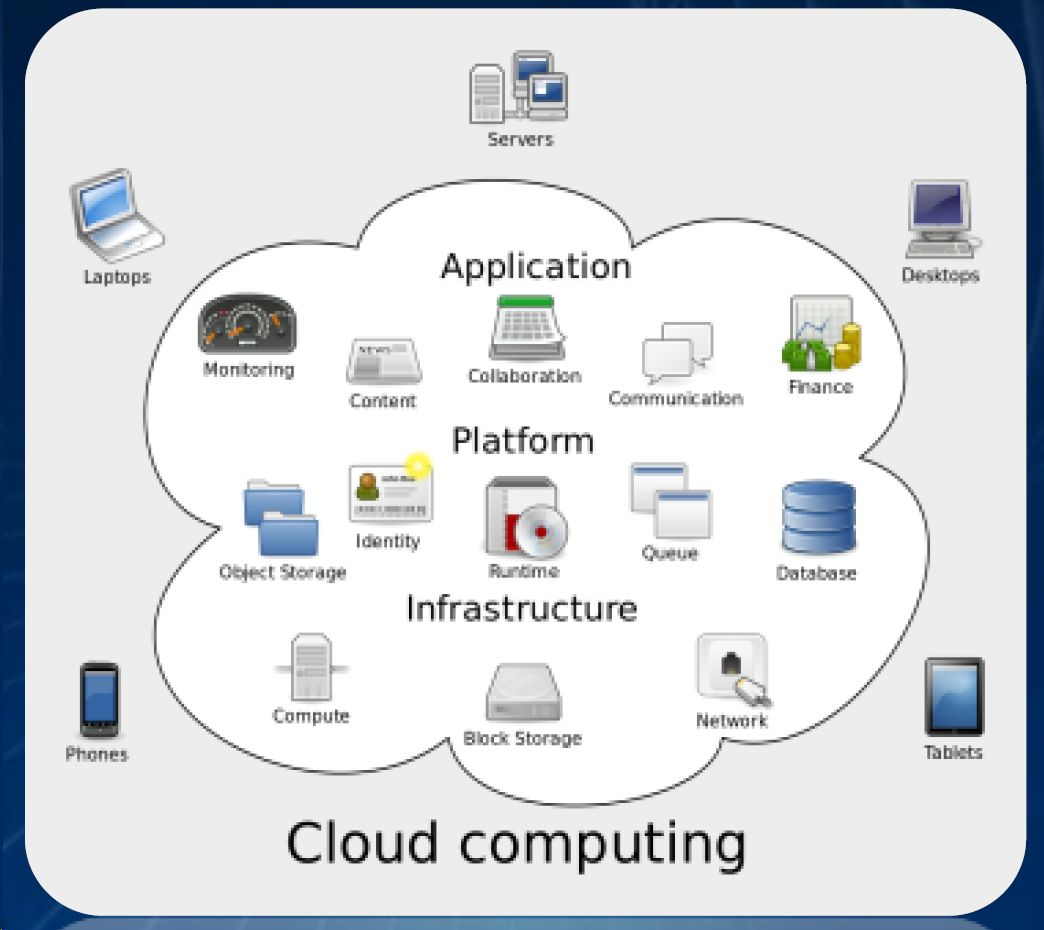
\includegraphics[width=0.7\textwidth]{images/17_lez_fig_01.jpg}
    \caption{Schema dei servizi e modelli del cloud computing.}
    \label{fig:cloud-computing}
\end{figure}

Ecco, vedete cloud computing o nuvola informatica. Ci sono infrastrutture, piattaforme e applicazioni sulle quali vengono gestite le attività più varie, dalla gestione dell'identità, all'archiviazione di oggetti, alla gestione delle reti, attività di collaborazione e quant'altro. 
Alla nuvola accedono i dispositivi più diversi, i server, laptops, telefoni smartphone, tablets e desktop. 

Vediamo adesso un video con delle immagini interessanti che nella maniera migliore può farvi comprendere che cos'è il cloud computing. 

\section{Video e traduzione}
\textit{Hi, today we're going to talk about cloud computing and level 3 communications. It used to be that your key business applications were just down the hall, across the campus, or at your company's headquarters. But now, with cloud computing, business applications, storage, computing cycles, networks, and other services are delivered to users virtually, or in the cloud. 
As your business increasingly relies on cloud computing for services and applications, how do you make sure those applications are as secure and perform as well as they did when they were on your dedicated local or wide area network? That's where the network comes in. Let me explain. Let's start with defining the cloud. Basically, the cloud is a way of delivering applications and IT resources. It's made up of a network of connections that provide access to services and a way for providers to deliver services to users. When you hear someone talk about the cloud, most of the time they are referring to IT services delivered via the public internet. However, many kinds of networks can be referred to as the cloud. There are public clouds based on the public internet, private clouds based on private internets, and hybrid clouds that combine the two. 
Because of the number of versions of the cloud, not everyone is happy with the same one. You might be using an application like email that works fine with the varying performance of the public cloud, but certain users like government agencies, financial institutions, and healthcare providers, to name a few, have serious concerns about privacy and security on the public internet. Not only do users have different needs, but the applications delivered over the cloud have different performance needs as well. What if, for example, you want to use the cloud for telemedicine or to store sensitive data? Would you want your doctor to trust your medical care to a best effort network? With compliance and privacy issues, consistent, secure performance is critical. As businesses migrate more and more critical business functions to the cloud, choosing the right cloud becomes essential. The better the cloud delivers your application and resources, the better your experience. 
If you're planning to use the public cloud, you'll want an internet service provider that can provide high performance and reliability. Level 3 has one of the most connected networks in the world. 60\% of all traffic that originates on the level 3 IP network stays on net. It's like your data is being carried in the express lane on the internet superhighway. When the public cloud simply isn't secure enough or performance is critical, financial institutions, government agencies, and other businesses might be more comfortable with a private cloud. 
This is where level 3 can help. We offer an extensive private IP network, along with other dedicated network options. This allows us to build private or hybrid clouds that offer all the benefits of IP, but with the security and performance of a private network. Cloud computing offers many benefits, but one size cloud does not fit all users. You need the right type of cloud network to support the way you want to use the cloud. 
At level 3, our network is built to offer scalability, performance, and security. 
We provide the platform for businesses to migrate critical applications to the cloud, no matter what type of cloud you require. For more information on cloud computing and how level 3 can help, check out www.level3.com forward slash cloud.}
\\
\\
Ciao, oggi parleremo del cloud computing e delle comunicazioni di Level 3. Un tempo, le applicazioni aziendali fondamentali si trovavano proprio dietro l’angolo, dall’altra parte del campus o nella sede centrale della tua azienda. Ma oggi, con il cloud computing, applicazioni aziendali, archiviazione, cicli di elaborazione, reti e altri servizi vengono forniti virtualmente agli utenti, ovvero nel cloud.

Man mano che la tua azienda si affida sempre più al cloud per servizi e applicazioni, come puoi assicurarti che tali applicazioni siano sicure e performanti quanto lo erano quando si trovavano sulla tua rete locale o su una rete geografica dedicata? È qui che entra in gioco la rete. Lascia che ti spieghi.

Iniziamo col definire il cloud. Fondamentalmente, il cloud è un modo per fornire applicazioni e risorse IT. È costituito da una rete di connessioni che consente l’accesso ai servizi e permette ai fornitori di consegnarli agli utenti. Quando senti parlare di cloud, nella maggior parte dei casi si fa riferimento a servizi IT forniti tramite internet pubblico. Tuttavia, ci sono vari tipi di reti che possono essere definite "cloud".

Esistono cloud pubblici basati su internet pubblico, cloud privati basati su reti private e cloud ibridi che combinano entrambi. A causa di questa varietà di versioni del cloud, non tutti sono soddisfatti della stessa soluzione. Potresti, ad esempio, usare un’applicazione come l’email che funziona bene anche con le prestazioni variabili del cloud pubblico. Tuttavia, alcuni utenti – come enti governativi, istituzioni finanziarie e operatori sanitari, solo per citarne alcuni – hanno serie preoccupazioni riguardo alla privacy e alla sicurezza su internet pubblico.

Non solo gli utenti hanno esigenze diverse, ma anche le applicazioni offerte tramite il cloud hanno requisiti di prestazione differenti. Cosa succede, ad esempio, se vuoi usare il cloud per la telemedicina o per archiviare dati sensibili? Vorresti davvero che il tuo medico si affidasse a una rete “best effort” per curarti? Con le problematiche di conformità e privacy, prestazioni sicure e costanti sono fondamentali.

Man mano che le aziende trasferiscono sempre più funzioni critiche nel cloud, scegliere il cloud giusto diventa essenziale. Più il cloud è efficiente nel fornire le tue applicazioni e risorse, migliore sarà la tua esperienza.

Se prevedi di usare il cloud pubblico, vorrai un provider di servizi internet in grado di garantire prestazioni elevate e affidabilità. Level 3 possiede una delle reti più interconnesse al mondo. Il 60\% di tutto il traffico che ha origine nella rete IP di Level 3 rimane all’interno della rete stessa. È come se i tuoi dati viaggiassero sulla corsia preferenziale dell’autostrada di internet.

Quando il cloud pubblico non è abbastanza sicuro o quando le prestazioni sono fondamentali, istituti finanziari, enti governativi e altre aziende potrebbero preferire un cloud privato. Ed è qui che Level 3 può aiutare. Offriamo un’ampia rete IP privata, insieme ad altre opzioni di rete dedicate. Questo ci consente di costruire cloud privati o ibridi che offrono tutti i vantaggi dell’IP, ma con la sicurezza e le prestazioni di una rete privata.

Il cloud computing offre molti vantaggi, ma una sola tipologia di cloud non è adatta a tutti gli utenti. Serve il tipo giusto di rete cloud per supportare il modo in cui intendi utilizzare il cloud. La nostra rete, in Level 3, è costruita per offrire scalabilità, prestazioni e sicurezza. Forniamo la piattaforma necessaria per consentire alle aziende di migrare applicazioni critiche nel cloud, indipendentemente dal tipo di cloud richiesto.

Per ulteriori informazioni sul cloud computing e su come Level 3 può aiutarti, visita www.level3.com/cloud.

Dal video emerge che il cloud è estremamente complesso e estremamente utile. 

\subsection{Caratteristiche da cui partire}
Quali sono le caratteristiche fondamentali da cui partire:

\begin{itemize}
    \item centralizzazione delle infrastrutture, delle piattaforme e dei programmi informatici, questo è il punto di partenza 
    \item redistribuzione agli utenti finali attraverso internet 
\end{itemize}

\subsection{Modelli di cloud computing}

I modelli noti di cloud sono:
\begin{itemize}
    \item il private cloud
    \item il public cloud
    \item il community cloud
\end{itemize}



Si tratta dei modelli attualmente esistenti, sui quali si fa una distinzione in base agli utenti che possono accedere al sistema. 

\subsubsection{Private cloud}
Nel caso del private cloud, l'infrastruttura è dedicata alle esigenze di un'unica organizzazione e può essere gestita in proprio, in house, oppure può essere gestita da un soggetto esterno che fornisce servizi esclusivamente al cliente, al soggetto che gli ha richiesti. Il private cloud permette di consolidare un'infrastruttura e le applicazioni informatiche che sono necessarie per la gestione delle risorse e per l'erogazione dei servizi a vantaggio di un aumento significativo di efficienza e di efficacia. La scelta della tecnologia da adottare è affidata al responsabile informatico delle singole organizzazioni, in base alle esigenze dell'organizzazione, e può essere dedicata all'infrastruttura a soggetti privati o a soggetti pubblici. 
Quindi si parla di private cloud perché è dedicato ad un unico soggetto e non è aperta ad altri.

\subsubsection{Public cloud}
Nel caso invece del public cloud, l'infrastruttura è di proprietà di un fornitore specializzato in questo specifico ambito tecnologico e il fornitore mette a disposizione degli utenti le risorse utilizzabili per la gestione di attività finali. Sostanzialmente si tratta di un'erogazione di servizi via web e la messa a disposizione di un ambiente nel quale possono essere conservati i dati e al quale si può accedere agevolmente attraverso i propri dispositivi. L'esempio tipico di public cloud è legato ad esempio alla fornitura di web server mail, quindi servizi di posta elettronica a cui si accede direttamente attraverso il web. Il public cloud è generalmente diretto a una molteplicità di utenti che non hanno alcun tipo di rapporto fra loro. 

\subsubsection{Community cloud}
Nel caso invece della community cloud, l'infrastruttura è utilizzata da più utenti che hanno fra di loro degli elementi comuni. Può essere ad esempio una specifica comunità che ha le stesse esigenze e che decide di condividere, di centralizzare, la fornitura dei servizi informatici. L'infrastruttura anche in questo caso può essere gestita dalla stessa comunità oppure anche in questo caso da un fornitore esterno che mette a disposizione le proprie attività, le proprie competenze, i propri servizi a favore della comunità. 

\subsubsection{Cloud intermedi}
Esistono anche dei cosiddetti cloud intermedi nei quali si utilizzano alcune delle caratteristiche di uno, alcune delle caratteristiche dell'altro. 

\subsection{Modelli di servizio}

\begin{itemize}
    \item IAAS, Infrastructure as a Service. In questo caso il fornitore mette a disposizione un'infrastruttura in sostituzione o in aggiunta a sistemi che l'utente ha già a disposizione. Le risorse messe a disposizione dell'utente non sono predefinite, ma sono individuate di volta in volta a seconda delle effettive esigenze che si presentano al momento
    \item SAAS, Software as a Service. In questo caso il fornitore eroga direttamente i servizi, spesso in sostituzione di quelli già installati degli utenti sui loro sistemi e fra i software più diffusi vi sono i fogli di calcolo e gli strumenti per l'elaborazione di testi, di applicazioni di protocollo informatico, per rubriche di contatti, calendari condivisi, sistemi di posta elettronica.
    \item PAAS, Platform as a Service. Nel caso della platform as a service il fornitore offre degli strumenti per sviluppare ed ospitare delle applicazioni nuove ed è un tipo di servizio dedicato soprattutto agli sviluppatori di sistemi. Lo sviluppatore accede alla piattaforma e sulla base di quella sviluppa servizi ulteriori che poi fornisce al soggetto finale. 
\end{itemize}   

Ecco una slide \ref{fig:Cloud_services} che vi può chiarire meglio il funzionamento dei modelli di servizio   

\begin{figure}[ht!]
    \centering
    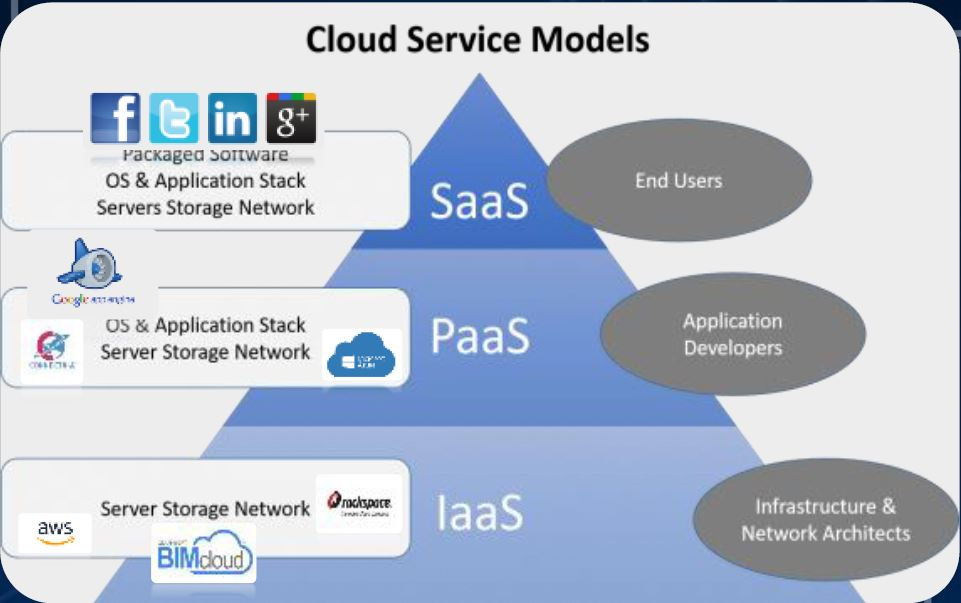
\includegraphics[width=0.7\textwidth]{images/17_lez_fig_02}
    \label{fig:Cloud_services}
    \caption{Cloud services}
\end{figure}

Vedete IAAS, Infrastructure and Network Architecture, trovate qui dei fornitori così per così dire di base, al secondo livello della piramide ci sono gli sviluppatori delle applicazioni, all'ultimo livello della piramide ci sono gli utenti finali che accedono attraverso servizi offerti al pubblico. 

\subsection{Vantaggi del cloud}
Il cloud presenta vantaggi e rischi. 
Vediamo prima di tutto quali sono i vantaggi che sono quelli che hanno portato a una diffusione assolutamente enorme nel mondo odierno dei servizi in cloud: 

\begin{itemize}
    \item acquisire servizi al posto di acquisire beni con quello che questo comporta dal punto di vista economico
    \item gestione dell'infrastruttura semplificata, effettuata da altri
    \item possibilità di avere un archivio senza limiti di spazio
    \item la possibilità di usufruire di economie di scala
\end{itemize}

Va considerato che la gestione dei sistemi informatici, l'acquisto di sistemi informatici, la loro manutenzione nel corso del tempo, ha dei costi estremamente elevati. 

Una delle caratteristiche della tecnologia moderna è quella di avere un'obsolescenza rapidissima e quindi la necessità di aggiornamento e di adeguamento dei sistemi, sia hardware che software, è una necessità molto forte con richiesta di aggiornamento che è sempre più rapida. Rimanere al passo con i tempi e con gli aggiornamenti richiede degli investimenti economici molto impegnativi. 

La possibilità di accedere a sistemi in cloud consente di ridurre enormemente i costi perché quello che si acquista non è un oggetto, ma sono delle attività, sono dei servizi. 
Quello che si acquista è una licenza di utilizzo, se ci sono degli aggiornamenti che vengono fatti dal fornitore questi aggiornamenti verranno resi disponibili senza necessità di acquisti nuovi ma semplicemente rinnovando e continuando ad avere delle licenze aggiornate. 
Il tema dei costi è un tema fondamentale nella gestione. 

Un altro tema è quello dello spazio, l'archiviazione delle informazioni e dei dati che comunemente si utilizzano nella gestione quotidiana delle attività è enorme. Lo spazio di memorizzazione che si richiedeva un tempo era poca cosa perché si archiviavano soprattutto dati semplici. Oggi con l'utilizzo di programmi complessi e con l'utilizzo di documenti di tipo diverso che prevedono audio, video, prevedono oggetti di grande peso che richiedono un spazio di memoria notevole, anche avere i dispositivi per l'archiviazione ha dei costi e delle richieste di implementazione costante. Anche in questo caso avere a disposizione uno spazio di archiviazione senza la necessità di acquisire la macchina su cui l'archiviazione va effettuata consente di ridurre i costi. 

Altro aspetto riguarda anche la possibilità di fare delle economie di scala. Lo sviluppo di un sistema informatizzato di gestione delle attività personalizzato sul soggetto, sull'organizzazione che ne deve usufruire può avere dei costi anche esso molto elevati. L'utilizzo invece di sistemi sviluppati e resi disponibili a più soggetti consente di facilitare, di dover riflettere meno su quelle che sono le esigenze ma di trovare già un prodotto pronto e anche questo permette delle notevoli economie di scala. Questi sono i vantaggi che hanno portato a uno sviluppo continuo dell'utilizzo dei cloud. 

\begin{figure}[ht!]
    \centering
    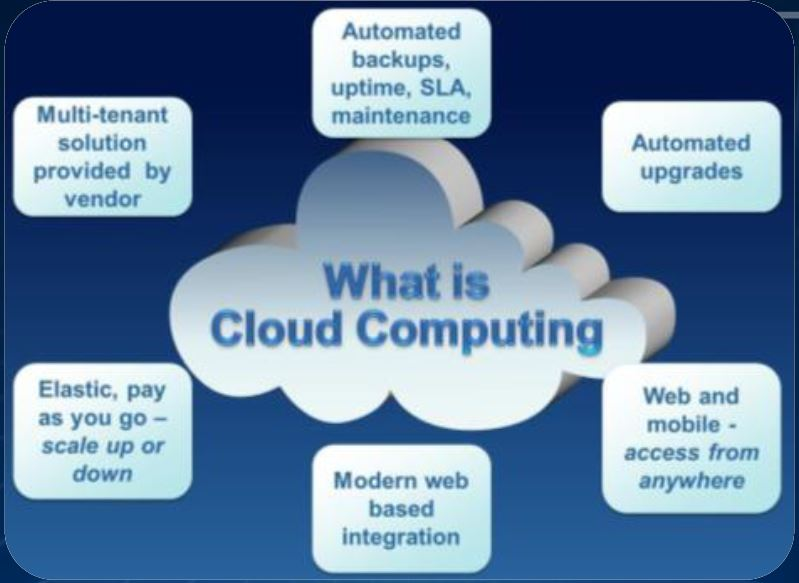
\includegraphics[width=0.7\textwidth]{images/17_lez_fig_03}
    \caption{Vantaggi Cloud}
    \label{fig:Vantaggi_Cloud}
\end{figure}

su questa slide \ref{fig:Vantaggi_Cloud} vedete quali sono le caratteristiche principali e gli aspetti positivi.

\subsection{Rischi del cloud}

Ci sono ovviamente come in tutto ciò che riguarda la tecnologia anche dei rischi. 
Vediamo quindi adesso quali possono essere i rischi dell'utilizzo del cloud:

\begin{itemize}
    \item perdita di controllo sui dati. Il fatto di archiviare i dati su uno spazio che non è proprio ha delle possibilità di rischio rispetto alla loro perdita e questo è un primo tema.
    \item  concentrazione dei dati. Normalmente i soggetti che forniscono servizi in cloud e che quindi archiviano i dati di proprietà dei clienti finali prevedono e provvedono all'archiviazione di dati di più soggetti, di più entità organizzative. Questo significa che in capo ai soggetti, ai fornitori di servizi cloud, si concentrano enormi numeri di dati di più soggetti con il rischio di commistione dei dati se non c'è un sistema di sicurezza adeguato e con il rischio comunque che chi detiene la conservazione dei dati ha un potere immenso perché i dati oggi nella società delle informazioni di oggi sono una ricchezza enorme.
    \item collocazione sconosciuta dei dati. Nel momento in cui noi mettiamo i nostri dati in cloud non sappiamo esattamente dove sono conservati questi dati, dove sono posizionati i server. Nel contratto normalmente è indicato dove sono collocati i server sui quali dati sono archiviati ma la società, il soggetto che fornisce questi servizi nel corso del tempo può subire dei mutamenti e quindi può accadere che questi dati vengano trasferiti altrove. L'utente finale, il cliente che usufruisce dei servizi non sempre può essere messo in condizioni di conoscere dove i propri dati sono archiviati e questo è un tema delicato da trattare. 
    \item  interoperabilità. Il conferimento dei dati su un certo sistema di cloud con determinate modalità può in qualche modo avere dei vincoli. Per avere la disponibilità continua dei propri dati e poter anche decidere di cambiare il fornitore, occorre che i dati vengano conservati in maniera tale che si possano spostare da un punto all'altro. Occorre la possibilità di gestire gli stessi dati anche con un sistema diverso senza avere una perdita. Quindi il tema della interoperabilità è un tema fondamentale nella gestione del cloud.
\end{itemize}

Il primo spunto di riflessione. In cosa consiste il cloud computing? 
%19:40

\section{Cloud computing sostenibile nella strategia europea}

L'importanza che la gestione del cloud ha assunto nel corso degli anni ha portato l'Unione Europea ad occuparsene con diversi programmi di azione. L'Europa ha elaborato delle strategie. 

La strategia generale europea per il cloud computer comporta diversi punti di vista e diverse azioni. 

\begin{figure}[ht!]
    \centering
    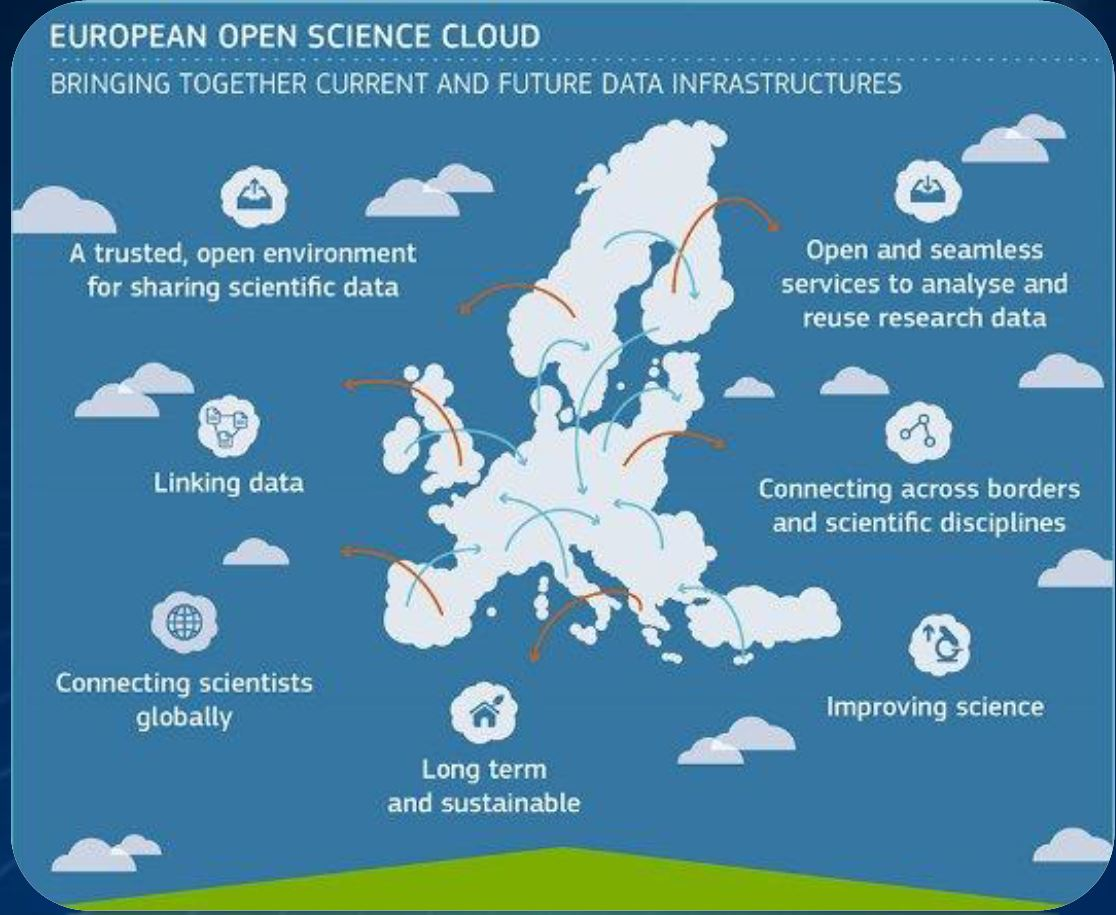
\includegraphics[width=0.7\textwidth]{images/17_lez_fig_04}
    \caption{European open science cloud}
    \label{fig:European}
\end{figure}

Rissumendo possiamo dire che occorre:
\begin{itemize}
    \item un ambiente aperto e affidabile per la condivisione di dati scientifici
    \item un ambiente aperto e gestibile per consentire l'analisi e il riuso dei dati di ricerca
    \item avere delle possibilità di collegamento semplice
    \item andare oltre quelli che sono i confini per poter condividere i dati
    \item una connessione globale tra gli scienziati
    \item una strategia a lungo termine sostenibile
    \item aiutare l'incremento della scienza
\end{itemize}

\subsection{Mercato unico digitale europeo}
La strategia europea attuale passa per un concetto di mercato unico digitale europeo. In questo contesto di mercato unico digitale europeo il cloud computing ha un ruolo chiave per la realizzazione di una data economy europea, di un'economia europea dei dati. 

La realizzazione del mercato unico digitale europeo passa attraverso una regolamentazione ma anche l'adozione, diffusione ed adozione di codici di condotta autoregolatori. 

\subsection{Progetti europei per il cloud}
Un primo progetto europeo, la strategia europea del 2012 per il cloud computing ha fatto partire una serie di iniziative. 

Oggi abbiamo il progetto Horizon 2020 che sta portando avanti i concetti del cloud computing. 

Quindi l'Unione Europea è ormai da diversi anni che si sta occupando di questo tema e nell'occuparsene ha individuato alcuni punti di riferimento fondamentali attraverso i quali bisogna passare per arrivare a quegli obiettivi che abbiamo visto prima. Di base sostanzialmente il concetto è che deve esserci una possibilità di condivisione semplice dei dati all'interno dell'Unione Europea, in particolare dei dati che sono conoscibili a tutti, deve essere possibile consentire a tutti di usufruire della stessa tipologia di servizi in maniera uniforme all'interno dell'Europa, quindi senza digital divide all'interno dei vari paesi europei. Per far questo è stato necessario e occorre continuare a sviluppare delle politiche comuni individuando dei punti di riferimento comuni a cui si possa accedere per proseguire con lo sviluppo. 

Potrete vedere tra i materiali che vi saranno messi a disposizione che ci sono proprio dei siti dedicati dell'Unione Europea proprio per il tema del mercato digitale sostenibile su cui sarà possibile fare degli approfondimenti. 

Vediamo in sintesi quali sono i temi fondamentali. Un cloud computing sostenibile:

\begin{itemize}
    \item richiede l'adozione di regole sicure, uniformi e semplici. Parlare di regole sicure, uniformi e semplici vuol dire uniformare una regolamentazione che è una regolamentazione sostanzialmente giuridica. Abbiamo accennato prima il fatto e poi, tra poco ne parleremo meglio, alla necessità di stipulare dei contratti per accedere ai servizi di cloud. Vedremo tra poco che l'utilizzo del cloud chiama in considerazione una serie di elementi che sono disciplinati da un punto di vista giuridico. Vedremo che abbiamo un tema di trattamento di dati personali, vedremo che abbiamo un tema di gestione dei rapporti contrattuali, vedremo che abbiamo un tema di sicurezza informatica che passa anche attraverso problematiche normative proprio di cyber crime. Quindi c'è un tema giuridico da tenere in considerazione sul quale occorre un'uniformità regolatoria. 
    \item richiede la semplificazione degli standard tecnici. Gestione del cloud è tecnologia e quindi per ottenere una facile circolazione, una facile interoperabilità, occorre avere degli standard tecnici semplificati e condivisibili, quindi due aspetti giuridico e tecnico che non possono in nessun caso essere divisi. 
    \item portabilità dei dati e delle informazioni. Ricordiamoci che i dati, una volta che sono stati strutturati, perché sono stati inseriti all'interno di un sistema, diventano meno flessibili. Per recuperarli e passare ad un sistema diverso, occorre che ci sia la possibilità di uscire, per così dire, da quella che è la struttura nella quale sono inseriti.
    \item interoperabilità
    \item reversibilità, possibilità di tornare indietro nelle informazioni che vengono inserite
\end{itemize}

Quindi l'elaborazione di standard tecnici richiede di tenere in considerazione queste tre caratteristiche, portabilità, interoperabilità, reversibilità. 

Un altro spunto di riflessione: quali sono le regole per un cloud computing sostenibile? 

\section{L'inquadramento giuridico del cloud computing}
Passiamo ora al terzo argomento, l'inquadramento giuridico. L'inquadramento giuridico del cloud computing è determinante per un cloud sostenibile. Per quanto riguarda il fornitore dei servizi di cloud, il fornitore deve:

\begin{itemize}
    \item fornire servizi e consentire l'accesso alla rete
    \item dotarsi di regole contrattuali, gestibili e utilizzabili
    \item occorre prevedere una ripartizione di ruoli e responsabilità nella gestione
\end{itemize}


La disponibilità dei dati e la loro accessibilità in qualunque momento richiede innanzitutto una certezza del livello della connettività. Occorre essere sicuri che sia sempre possibile accedere a quei dati. Provate ad immaginare per un'azienda che decide di usufruire di un servizio in cloud e che quindi archivia tutti i dati che le servono ordinariamente per la gestione dell'azienda su un server cloud e che quotidianamente accede al cloud per la gestione delle attività ordinarie, provate ad immaginarvi se per mezza giornata non è in grado di accedere alle proprie risorse. Questo può creare dei danni anche economici enormi. Quindi occorre avere una certezza sul livello di connettività e la possibilità di accedere ai servizi. È chiaro che l'accesso ai servizi, l'accesso ai dati archiviati, da un lato richiede un'attività del fornitore del servizio, dall'altro passa attraverso l'infrastruttura, cioè attraverso il soggetto che fornisce il servizio di connettività alla rete che normalmente è diverso dal fornitore del cloud. Qua si pone un tema ulteriore e diverso nel quale interviene un soggetto diverso dal fornitore del cloud. 

C'è un tema fondamentale di parità nella possibilità di accesso alle risorse che è in discussione continua. Proprio tra la fine del 2017 e l'inizio del 2018 negli Stati Uniti si è posto il tema della neutralità della rete. Neutralità della rete di cui uno degli aspetti è proprio quello di poter accedere alle risorse indipendentemente da quanto si paga l'accesso alle risorse. Questo è un tema che è importantissimo e che diventerà sempre più importante. 

Secondo tema, come avete visto, sono le regole contrattuali. Nel momento in cui un cliente finale decide di usufruire di servizi informatici in cloud,  di stabilire un rapporto con un fornitore di servizi, lo fa attraverso la stipula di un contratto. 

Contratto che sarà regolato forse dalla normativa nazionale, nella nazione in cui risiede il cliente finale, ma che potrebbe invece essere regolato da normativa diversa se il fornitore dei servizi cloud risiede in un altro luogo. Vedremo fra poco che il tema della giurisdizione, della normativa applicabile, della giurisdizione competente è un tema da affrontare nella parte più concreta, nella gestione più concreta delle attività. 

Ancora, e qua torno al tema del rapporto fra disponibilità del servizio e infrastruttura che mi consente di accedere al servizio, c'è un tema di ripartizione di ruoli e responsabilità per cui se il cliente finale ha un problema deve sapere con chi prendersela. Anche questo aspetto è un aspetto che può essere definito a livello contrattuale ma che può essere definito invece a livello di regolazione generale, normativa generale. 

Altro tema è la sicurezza. Occorre che vi sia un accesso a dati certi e che questi dati siano sempre integri. Il tema dell'accesso e dell'integrità dei dati tocca da un lato il trattamento dei dati personali, dall'altro un tema di sicurezza rispetto alla tutela dei reati informatici.

In entrambi questi casi abbiamo delle normative specifiche. 

Per quanto riguarda il trattamento dei dati personali richiamo il regolamento generale sul trattamento dei dati personali elaborato dall'Unione Europea ed entrato pienamente in vigore nella primavera del 2018. 

Per quanto riguarda i reati informatici, parlando di normativa di carattere internazionale, mi riferisco come punto di riferimento base alla convenzione sul cybercrime elaborata ed emessa a Budapest nel 2001 e che è stata attuata da quasi tutti gli Stati Europei. 

Altro tema è quello della proprietà dei dati, proprietà intellettuale innanzitutto verso open data. 

Quando parliamo di proprietà dei dati parliamo di diversi aspetti. È proprio oggetto di discussione in Unione Europea nella primavera e estate del 2018 una modifica della normativa sul diritto d'autore che ha delle previsioni particolari e che vuole tenere conto delle caratteristiche delle complessità del web. 

Parleremo di questo tema in una prossima lezione. Qua basti dire che il tema della proprietà intellettuale dei dati è un tema che si pone in modo fondamentale nel momento in cui io organizzazione, io soggetto, io cliente finale, conferisco, inserisco i dati all'interno di un sistema di archiviazione di cloud non per questo cedo la proprietà dei miei dati e questo comporta una valutazione, un'elaborazione di norme contrattuali e norme generali che mi consentano di garantirmi rispetto al furto di questi dati o all'utilizzo di questi dati non adeguato. 

Questo è un tema molto dibattuto in rapporto a quelli che sono i cosiddetti open data, cioè i dati che escono in qualche modo dalla sfera di chi quei dati li ha elaborati e di chi è il proprietario dei dati e che vengono messi a disposizione del pubblico. La gestione degli open data è una gestione particolare e articolata che tiene conto di diverse esigenze. 

Si tende a considerare open data quelli che sono i dati di interesse pubblico, si tende a pensare agli open data quando il titolare, il proprietario del dato, ritiene che sia possibile metterli a disposizione della collettività. In entrambi i casi vi sono delle normative specifiche condivise a livello internazionale. 

Collocazione e trasferimento dei dati. Abbiamo accennato prima il fatto che i dati non sappiamo dove esattamente vengono collocati. Si pone quindi un tema di giurisdizione, nel caso di contenziosi, e di competenza. 

Altro tema, ne abbiamo accennato prima, è quello dei big data. La conservazione di una grande quantità di dati presso un unico soggetto può porre delle tematiche di concorrenza, può porre delle tematiche di controllo, può porre una serie di temi da affrontare nel momento in cui sono gestite grandi, grandissime masse di dati. 

Ulteriore tema è quello della conservazione. Conservazione dei dati durante il rapporto contrattuale e dopo la scadenza del contratto. Abbiamo visto che nel momento in cui si accede ad un sistema di cloud, nei momenti in cui si archiviano i dati in un cloud, questi dati vengono appoggiati in un sistema di conservazione che esce al di fuori della sfera di disponibilità del soggetto che è proprietario di quei dati o che comunque legittimamente li detiene. Questi dati vengono affidati ad un soggetto terzo in base ad un rapporto contrattuale che stabilisce la regolamentazione del rapporto nella fornitura del servizio e quindi durante quel rapporto contrattuale occorre assicurarsi che i dati vengano conservati in sicurezza, che vengono conservati in maniera da non essere accessibili a terzi che non sono autorizzati a prenderli e ad accedere. Occorre assicurarsi che quei dati vengano messi a disposizione quando c'è la richiesta di accesso a quei dati. 

Nel momento in cui il rapporto contrattuale si chiude, occorre verificare cosa succederà di quei dati. Tipicamente questi dati dovrebbero essere rimessi a disposizione del cliente finale, il quale potrebbe decidere di avvalersi di un altro fornitore. 

Quindi questa parte di gestione dei dati dopo la scadenza del contratto va verificata e disciplinata. 

Avete visto che la gestione del cloud è una gestione complessa dal punto di vista normativo.

Abbiamo visto tra le complessità del mondo moderno vantaggi e svantaggi nell'utilizzo dei sistemi di cloud computing. Ricordiamoci che questi sistemi sono dei sistemi che ormai sono ovunque, sono diffusissimi. Se vedete tutto ciò che chiunque di voi appoggia, per così dire, su uno smartphone, tutti i servizi a cui eccede attraverso uno smartphone, si può rendere conto di come la vita oggi si basi su servizi di cloud. È un sistema eccellente, ma occorre sapere di quali sono le tematiche, quali sono i rischi a cui si va incontro.

Spunto di riflessione: Cosa deve garantire il fornitore di servizi di cloud per rassicurare e assicurare il cliente? 

Abbiamo visto tutta la complessità della gestione del cloud computing e qui facciamo un riassunto, un riepilogo degli spunti di riflessione: 
In cosa consiste il cloud computing? 
Quali regole sono state individuate per un cloud computing sostenibile? 
Cosa deve garantire il fornitore di servizi di cloud? La nostra lezione termina qui. 
\chapter{Lezione 18 - Computer Crimes e Computer Forensics}

L'argomento della lezione di oggi è Computer Crimes e Computer Forensics.

\section{Computer Crimes}
Per Computer Crimes o diritto penale dell'informatica si intende in generale la rilevanza dell'informatica nel diritto penale. Questo può avvenire in due ordini di fatti specie. La prima tipologia di fatti specie di diritto penale dell'informatica sono i reati comuni commessi con strumenti informatici.Vale a dire, tutta una serie di reati comuni, reati che possono essere commessi nel mondo reale, con strumenti fisici o comunque con strumenti non informatici che  possono anche essere commessi con strumenti informatici. 

Questo accade per esempio con violazioni della privacy, effettuate con strumenti informatici, cosa che non è necessario avvenga con strumenti informatici. La privacy può essere violata in altre modalità. 

E' il caso della diffamazione online. La diffamazione è un reato che nasce nel mondo della stampa o con la comunicazione orale e così via. E' possibile ovviamente, siccome gli strumenti della socità dell'informazione diffondono informazioni, diffondono anche opinioni, idee, manifestazioni e pensieri, è possibile che la diffamazione avvenga online tramite internet.

La pedopornografia si è attuata con strumenti informatici. 
Quindi questi sono esempi di reati comuni che possono essere commessi con strumenti informatici. 

Altre altre famiglie di fattispecie riconducibili al diritto penale dell'informatica, invece, sono reati informatici in senso stretto. Vale a dire reati compiuti in danno di sistemi informatici. In questo tipo di reati il sistema informatico o l'informatica, il bene informatico, è il bene oggetto di protezione penale ed è ciò che la normativa penale intende proteggere.
Quindi in questa seconda famiglia di fattispecie, la norma penale intende proteggere un bene che ha qualità informatica, quindi ad esempio accesso abusivo a banche dati, accesso abusivo a sistema informatico, contraffazione di software e così via. Il bene giuridico che la norma penale protegge ha una natura informatica. A differenza, invece, della fattispecie del primo tipo in cui il bene giuridico è un bene giuridico normale, che fa parte della vita reale e la lesione al bene giuridico avviene tramite strumenti informatici. 

In Italia abbiamo avuto una normativa apposita sui reati informatici abbastanza recentemente. Mentre i primi provvedimenti negli Stati Uniti ci sono già dagli anni 80, il primo del 1984, poi un secondo importante provvimento è del 1986, solo successivamente il Consiglio di Europa ha emanato la raccomandazione 89 che raccomanda ai Paesi membri di adottare normative specifiche sulla protezione di beni aventi di tipo informatico o comunque sul diritto penale dell'informatica. 

In Italia è stata necessaria una nuova normativa che è arrivata nei primi anni 90. Era necessaria perché era difficile estendere in via interpretativa le disposizioni preesistenti, quelle previste dal codice penale o da altre disposizioni penalistiche fuori dal codice, ai beni di cui stiamo parlando per due motivi; in primo luogo perché il diritto penale italiano è retto dal principio di stretta legalità, vale a dire affinché una certa condotta sia sanzionata penalmente sia punibile con una pena, è necessario che quella condotta sia tipizzata in una fattispecie legislativa, quindi è necessario che il legislatore abbia preso esattamente in esame quel tipo di condotta. Questo per i molti beni come quelli di tipo informatico mancava. 

Vi erano delle lacune per esempio per la repressione penale dell'accesso abusivo ad una banca dati o a un sistema informatico. Inoltre, secondo aspetto, risultava talvolta difficile estendere in via interpretativa le normative esistenti su alcuni reati, nel momento in cui il reato stesso fosse stato commesso con strumenti informatici. 

Quindi si poneva il problema se la frode informatica potesse essere qualificata deplano, senza problemi di sorta, come un tipo di truffa; quindi se fosse legittima questa interpretazione estensiva o se invece stessimo versando in un'ipotesi di estensione analogica che per il diritto penale è vietata. 

Stesso dubbio poteva porsi, per esempio, sulla possibilità di estendere le tutele penali sul segreto della corrispondenza a forme di corrispondenza non cartacee, forme di corrispondenza diverse, che potrebbero essere quelle che si verificano su internet; quindi per evitare il rischio o il dubbio che certe estensioni di reati preesistenti a nuove fatti specie avvenissero con un'operazione interpretativa qualificabile come analogia e l'analogia nel diritto penale è vietata, allora il legislatore ha ritenuto opportuno, in talunni casi, introdurre specifiche fatti specie penali o estendere normative preesistenti. 

La normativa principale che disciplina il diritto penale dell'informatica è quella introdotta dalla legge 547 del 1993. Questa legge in gran parte inserisce nuovi articoli o modifica articoli esistenti nel codice penale, quindi sono introdotti nel codice penale o nel corpo del codice penale degli articoli dedicati espressamente ai reati aventi a che fare con l'informatica. Questo è stato fatto secondo le due direttrici che menzionavo poc'anzi, vale a dire o con l'introduzione di nuove fatti specie, l'esempio è l'accesso abusivo al sistema informatico, o con l'estensione di fatti specie già esistenti. Quindi in alcuni casi sono state create delle figure di reato del tutto nuove, perché non vi era nulla che potesse plausibilmente somigliare nel codice penale preesistente a quella fattispecie nuova che riguarda la protezione di un bene informatico. 
Oppure, seconda modalità, presa a una disposizione del codice penale che disciplina una certa condotta, una certa fattispecie, questa fattispecie è stata è stata integrata espressamente dal legislatore con il riferimento a certi beni informatici. L'esempio è quello della violenza sulle cose, la violenza sulle cose si può esercitare su cose fisiche, su cose materiali e il legislatore ha esteso questa possibilità anche alla violenza su sistemi informatici, reti e quant'altro. 

Vediamo alcuni esempi specifici di reati aventi a che fare con l'informatica, sono tanti, ne vedremo solo alcuni e più interessanti. 

\subsection{Esempi di reati informatici}
\subsubsection{Frode informatica}
Il primo esempio è la froda informatica disciplinata dall'articolo 640ter del codice penale è considerato un tipo di truffa e in effetti come collocazione all'interno del codice si trova molto vicino alla truffa. La truffa è un reato che consiste nell'impiegare artifici o raggiri per indurre qualcuno in errore affinché compia qualcosa che beneficia ingiustamente l'autore della truffa e danneggia ingiustamente il soggetto truffato. Potremmo dire che la frode informatica è una sorta di truffa ai danni di un calcolatore, ai danni di un sistema informatico o di un programma. 
Come si verifica? Si realizza tramite alterazione del funzionamento di un sistema informatico, tramite alterazione dei delle informazioni o del software, quindi è come se con una frode informatica il truffato fosse un computer o un sistema informatico, alterando il modo in cui funziona il suo software o uno dei suoi software, oppure alterando i dati, le informazioni in esse contenuti. Questi sarebbero gli artifici o raggiri applicati al mondo informatico. 

È necessario affinché il reato si realizzi che l'autore della frode informatica realizzi o intenda realizzare un ingiusto profitto per sé e al contempo realizzi o intenda realizzare un danno ingiusto ad altri. È pertanto richiesta per questa figura il dolo specifico, è una figura di reato esclusivamente dolosa. 
Il dolo consiste nell'attuare le alterazioni del sistema o dei dati al fine di realizzare un ingiusto profitto o realizzare un danno ingiusto per altri.

\subsubsection{Accesso abusivo a sistema informatico}
Un altro esempio di reato informatico è l'accesso abusivo a sistema informatico, disciplinato dall'articolo 615ter del codice penale. È un reato collocato tra i delitti contro l'inviolabilità del domicilio. Quindi si considera che il sistema informatico sia equiparato al domicilio di quel soggetto. Entrare abusivamente nel sistema informatico di un certo soggetto è come entrare nel suo domicilio, come entrare a casa sua o nella sede del suo domicilio professionale. Sappiamo inoltre che la tutela del domicilio è una tutela rafforzata perché è considerata inviolabile dalla Costituzione. 
La Costituzione considera il domicilio inviolabile, quindi si giustifica una protezione penale del domicilio, ancorché informatico. L'accesso abusivo al sistema informatico può realizzarsi in due tipi di fattispecie a e b, per comodità espositiva, non è un'articolazione fatta dal codice:

\begin{itemize}
    \item a) La prima fattispecie è introdursi indebitamente, illegitamente in un sistema munito di misure di sicurezza
    \item b) La seconda fattispecie è mantenersi indebitamente all'interno di un sistema informatico contro la volontà dell'avente diritto, volontà che può essere espressa o tacita
\end{itemize}

Entrambe le fattispecie, ma soprattutto la fattispecie a, e lo sottolineo perché su questa che si è verificato qualche dubbo interpretativo sono necessariamente effettuate con strumenti elettronici. La formulazione testuale dell'articolo infatti dice che si introduce in un sistema informatico. Si è infatti posto il problema se possa considerarsi accesso abusivo ad un sistema informatico per esempio entrare nella stanza in cui ha sede un server, in cui hanno sede le apparecchieture informatiche di un soggetto o di un'azienda e così via. Secondo l'interpretazione letterale che normalmente nel diritto penale dovrebbe essere preferita, si dovrebbe in realtà configurare il reato, o meglio la consumazione del reato, nel momento in cui si accede al sistema con strumenti informatici. 

La condotta a, introdursi abusivamente in un sistema informatico, è di solito prodromica alla condotta B, cioè al mantenersi in un sistema informatico. Quindi si accede abusivamente al sistema informatico per poi fare qualcosa all'interno di quel sistema informatico, captare dati riservati, hackerare il sistema affinché quella macchina svolga certe operazioni a distanza e così via. Tuttavia non è vero il contrario, vale a dire la fattispecie b, mantenersi all'interno di un sistema informatico contro la volontà dell'avente diritto, può realizzarsi senza la fattispecie a. Vale a dire, ci si può mantenere indebitamente all'interno di un sistema informatico contro la volontà dell'avente diritto, senza che l'accesso sia stato abusivo. L'accesso potrebbe essere avvenuto col consenso del titolare dell'avente diritto sul sistema informatico. 

Supponiamo ad esempio che io porti un computer a riparare presso un centro d'assistenza. Il soggetto che fa assistenza e riparazioni accede al sistema col mio consenso, perché l'ho utilizzato io a effettuare le operazioni di riparazione. Supponiamo poi che però quel soggetto introduca un software spia, un spyware, all'interno del mio sistema. In questo modo si realizza un mantenersi abusivamente all'interno del sistema anche se l'accesso originario era stato valido, era stato effettuato lecitamente. 

Altro esempio potrebbe essere il fatto della condotta del dipendente che utilizza certi sistemi informatici dell'azienda in cui lavora, per esempio accede a banche dati e così via, al di là dell'orario di lavoro. Supponiamo che il dipendente abbia l'autorizzazione di accedere ai sistemi esclusivamente all'interno dell'orario di lavoro e supponiamo che acceda al di fuori dell'orario di lavoro. In questo caso ha avuto accesso all'interno dell'orario di lavoro quando aveva titolo di farlo, ma si è mantenuto oltre e quindi la sua condotta è diventata quella della fattispecie b. 

La disposizione penalistica richiede l'esistenza di misure di sicurezza. Diciamo che in un certo senso l'esistenza di misure di sicurezza è funzionale a far presumere una volontà del titolare del sistema di selezionare gli accessi leciti. Quindi il fatto stesso che il sistema è protetto da misure di sicurezza fa presumere che l'accesso al sistema da parte dei soggetti che il sistema di sicurezza non riconosce, per esempio non sono in possesso della password, fa presumere un accesso abusivo, fa presumere che l'accesso si sia verificato senza la volontà del titolare dei diritti sul sistema. 
Il reato si consuma nel momento in cui si superano le misure di protezione. Quindi non è necessario che chi ha effettuato l'accesso abusivo al sistema poi raccolga dati o prenda cognizione di dati più o meno riservati contenuti all'interno del sistema, affinché il reato si consumi e scatti la responsabilità penale, è sufficiente superare le misure di protezione di cui il sistema è dotato. 

\subsubsection{Accesso abusivo a sistema informatico: reato di pericolo}
E' un reato di pericolo. Cosa vuol dire? Vuol dire che la tutela penale è anticipata rispetto al verificarsi di un reale o di un qualsiasi danno o ingiusto profitto e così via. 
La differenza di quanto abbiamo visto con l'esempio precedente della froda informatica. I reati di pericolo sono quei reati contrassegnati da un'anticipazione della tutela penale. 
La tutela penale o la responsabilità penale scatta in un momento anticipato rispetto a quello in cui si verifica un danno apprezzabile. Si presume la dannosità di un certo comportamento o la pericolosità ire ipsa \footnote{"In re ipsa" indica che la natura del fatto o della situazione è di per sé prova di un danno o di una responsabilità.} di un certo comportamento. 
Accedendo abusivamente ad un sistema informatico si compie la condotta penalmente rilevante anche se poi dentro quel sistema informatico non si è svolta nessuna operazione o anche se non si è in grado di provare quali siano le operazioni poi svolte all'interno del sistema informatico in cui si è praticato l'accesso abusivo.

È possibile che questo reato si presenti sotto la forma del tentativo, quindi reato consumato, reato tentato. Questo reato può verificarsi sotto la forma del tentativo. Come? Per esempio, se semplicemente si cerca di forzare le misure di protezione del sistema senza riuscirci, per esempio fare ingresso nei locali fisici in cui sono custoditi gli elaboratori protetti da misure informatiche di sicurezza. L'accedere ai locali dove sono custoditi elaboratori elettronici, sistemi informatici, può configurare, se il contesto consente questa interpretazione, quindi i mezzi idonei, un tentativo di accesso abusivo. 


\subsubsection{Diffusione di virus informatici}
Diffusione di virus informatici, articolo 615, quinques. 

Si intende per diffusione di virus informatici la diffusione, ovvero la comunicazione, la trasmissione, la registrazione di un programma informatico che ha per scopo o effetto il danneggiamento, l'interruzione, l'alterazione, o comunque l'interferenza con programmi informatici, con il loro funzionamento, con i dati che essi contengono, eccetera, eccetera. 
La fattispecie di diffusione di virus informatici richiede che il virus, quindi il programma destinato a interferire con altri programmi, sia effettivamente messo in circolo. Quindi sia comunicato individualmente a qualcuno, o sia diffuso con strumenti di un certo tipo. 
Affinché scatti la responsabilità penale non è necessario che un certo virus informatico sia stato prodotto o detenuto da un soggetto. Quindi, ammesso che io ne abbia la capacità tecnica, non commetterei un reato se progettassi un virus nel chiuso del mio studio, senza mettere in circolazione questo virus. D'altro canto, affinché scatti la responsabilità penale non è necessario che il virus sia stato prodotto da chi lo trasmette. 
Quindi è penalmente responsabile per diffusione di virus informatici chi trasmette, comunica, diffonde, i virus informatici anche se non li ha prodotti lui, anche se non sono stati prodotti in proprio. 

Un problema relativo a questa norma. La norma non richiede dolo specifico, ma solo dolo generico. Di conseguenza il dolo specifico sarebbe la volontarietà di trasmettere un virus, cioè la volontà di provocare un'interferenza, un danno e quant'altro, con un sistema informatico altrui o un danneggiamento dei dati che si contengono. La norma non richiede nulla di tutto ciò, non richiede questo dolo specifico. Di conseguenza c'è il rischio che un'interpreazione letterale di questa norma, di questa disposizione penalistica, dia luogo ad una eccessiva estensione dell'area della punibilità. A prima vista, infatti, potrebbe essere punito ai sensi della norma che stiamo commentando chi trasmette un virus ad una società informatica che si occupa di studiare virus, per progettare antivirus. Supponiamo che io mi accorga di avere un virus nel computer, lo trasferisco su un supporto, su un dischetto, su un CD, su un DVD  e trasmetto questo supporto che contiene il virus informatico ad una società specializzata in informatica che progetta sistemi antivirus dicendo, vi sto trasmettendo questo virus affinché lo analizziate. A prima vista questa condotta sembrerebbe ricadere nell'ambito della norma, quindi è necessario qualche tipo di interpretazione correttiva affinché la norma non punisca comportamenti che non hanno disvalore sociale. 

\subsubsection{Violazione della corrispondenza}
Esistono disposizioni penalistiche, in particolare l'articolo 616, che riguardano la tutela della corrispondenza. Ebbene questa disposizione è stata estesa a coprire anche la corrispondenza che si realizza con strumenti elettronici o informatici. 
Vediamo le fattispecie previste da questa norma. 

\begin{itemize}
    \item prendere cognizione del contenuto di una corrispondenza chiusa è reato ai sensi dell'articolo 616 del codice penale
    \item sottrarre o distrarre, al fine di prenderne conoscenza o farne prendere da altri cognizione, una corrispondenza chiusa o aperta. Quindi in questo caso l'oggetto della tutela è una corrispondenza o chiusa o aperta, che viene sottratta o distratta per prenderne cognizione o per farne prendere cognizione ad altri
    \item Terza fattispecie, distruggere o sopprimere in tutto o in parte una corrispondenza chiusa o aperta
\end{itemize}

Ebbene, in seguito ad una estensione operata espressamente da legislatore la disciplina penale di queste fattispecie si applica a qualunque forma di comunicazione a distanza, anche elettronica, per esempio email, chat, Skype, messaggeria su cellulari e quant'altro. Quindi la riservatezza di queste comunicazioni è tutelata dal codice penale nelle modalità che abbiamo visto. 

Abbiamo visto che le norme penali rilevanti fanno riferimento alla distinzione tra corrispondenza chiusa e aperta. La cassazione ha utilizzato, ai fini di distinguere tra le due fattispecie, cioè distinguere se versiamo in una fattispecie di corrispondenza chiusa o di corrispondenza aperta, ha utilizzato la circostanza del legittimo possesso della password. Quindi, se un soggetto prende cognizione di un messaggio di posta elettronica a lui non indirizzato, forzando la password, ovvero perché quella posta elettronica si trovava su un computer aperto disponibile, in questo caso commette l'illecito penale che abbiamo visto. 
Se invece la comunicazione elettronica viene conosciuta da un soggetto al quale la comunicazione non è indirizzata, ma quel soggetto dispone della password che permette di accedere a quella comunicazione elettronica, in tal modo non si realizza il reato che stiamo esaminando. 

Per esempio, questa fattispecie si verifica molto spesso sui loghi di lavoro nell'ipotesi del dipendente in ferie, ed è necessario accedere alla casella di posta elettronica di quel dipendente per lo svolgimento di certe pratiche o di certi affari precedentemente trattati da quel dipendente. Ora, il datore di lavoro o un suo incaricato che accede alla casella personale di posta elettronica del dipendente assente sta commettendo il reato di cui ci stiamo occupando? La soluzione è quella indicata dalla Cassazione. Se il datore di lavoro o l'incaricato detiene legittimamente la password per accedere a quella casella di posta elettronica, cioè l'interessato è stato debitamente informato del fatto che qualcun altro ha la password e potrà accedere, allora non si commette il reato di violazione della corrispondenza applicato alle caselle di posta elettronica. 

\section{Computer Forensics}

Per computer forensics o informatica forense si intende la ricerca di prove utilizzabili in giudizio attraverso il reperimento e l'analisi di sistemi informatici, reti, dati e quant'altro. Quindi è l'utilizzo di mezzi di ricerca della prova, che possono essere utilizzate in un giudizio penale. In realtà l'uso in giudizio penale è quello più frequente e anche quello oggetto di specifica normazione in Italia, ma nulla vieta che informazioni, dati di questo tipo, possono essere impiegati anche in un processo civile. 

Concentriamoci sul caso paradigmatico che è quello dell'uso nel processo penale. 
Quindi, la ricerca di prove utilizzabili in giudizio penale, quindi prove relative al compimento di un reato o a traccia di un reato, prove relative alla colpevolezza, prove relative alla complicità e quant'altro, attraverso il reperimento e l'analisi di sistemi informatici, di reti, di insieme di dati e così via. 

Questo tipo di attività è disciplinato adesso dalla legge 48 del 2008 che recepisce in Italia la Convenzione Europea sul Cybercrime e che ha determinato anche una serie di interventi, di modifiche al codice di procedura penale per tenere conto del ricorso a questo tipo di tecnologia nella ricerca della prova. 
%32:27
L'informatica Forense o Computer Forensics entra in gioco solo dopo che il reato è stato commesso, quindi non ha a che fare con misure di sicurezza o con finalità preventive o di anticipazione della commissione del reato. E' l'insieme delle misure, degli accorgimenti, degli strumenti che sono finalizzati all'accertamento e alla ricostruzione di un reato e della relativa responsabilità penale. 
Come si attua in pratica questo tipo di attività? 
Ad esempio, analisi di memoria di massa come hard disk, supporti rimovibili, CD, DVD e quant'altro. Oppure analisi di flussi di comunicazione di dati, quindi andando a ricostruire i rapporti, i flussi di informazione tra client e server, come sono transitati sulla rete e quant'altro. Si tratta quindi di un'attività di ricostruzione o su supporti hardware o su infrastrutture di rete. 

\subsection{Tecnicismo e digital divide processuale.}

Il problema con l'uso di queste tecniche è che sono tecniche spesso molto specialistiche, spesso sono sperimentali e controverse, la cui attendibilità, non è del tutto pacifica nella comunità degli utenti; quindi da un primo punto di vista l'uso di queste metodologie può essere controversa in giudizio e dare luogo a contestazioni dibattimentali. 

Da un secondo punto di vista può dare luogo a una sorta di digital divide processuale. Vale a dire, può esserci troppa distanza tra il tecnico, tra il modo tecnico in cui viene raccolta, viene formata la prova, in cui è stato predisposto il mezzo di ricerca della prova e le cognizioni delle parti e soprattutto del giudice. Quindi il giudice potrebbe essere inabilitato a vagliare in maniera attendibile il tipo di attività che è stato svolto per ricostruire la prova. Al limite il giudice potrebbe essere ostaggio del tecnicismo delle parti o dei loro consulenti, dei loro periti. 

Un problema che si è posto è se l'accertamento informatico, nelle varie modalità in cui si può svolgere, sia un accertamento ripetibile o non ripetibile. Un accertamento ripetibile è come dice la parola stessa un accertamento che può essere ripetuto indifferentemente tante volte. Un accertamento non ripetibile invece è un accertamento che o per la sua natura modifica le cose  oggetto dell'accertamento, oppure è un accertamento che si svolge su cose deperibili e così via. 

La differenza è rilevante perché nel caso di un accertamento non ripetibile sono necessarie tutta una serie di garanzie procedimentali che riguardano soprattutto il coinvolgimento del difensore, della parte che ha diritto a partecipare all'attività di accertamento, proprio perché non è più ripetibile. La Cassazione ha talvolta affermato che l'accertamento informatico non determina un'alterazione dello stato di cose perché si tratta di prendere conoscenza del contenuto per esempio dell'hard disk di un computer. 
Si tratta però di una ricostruzione errata perché è quasi inevitabile che i dati contenuti nella memoria di un computer, una volta che vi si acceda per fare un accertamento di questo tipo, vengono in qualche modo alterati. L'accertamento informatico di questo tipo quasi inevitabilmente determina un'alterazione dei dati contenuti. Affinché non determini questa alterazione è necessario prendere tutta una serie di accorgimenti specifici che non è scontato vengano adottati per esempio dalla Polizia Postale o dagli organi preposti. 

Esistono problemi specifici per quanto riguarda la conservazione, l'analisi e la presentazione dell'evidenza digitale. Si tratta esattamente di ciò che ho appena detto. È possibile che nell'acquisire i dati e nel conservarli i dati vengano alterati. Un'alterazione, una modifica dei dati può essere conseguente anche alle procedure di analisi, al modo in cui vengono analizzate. È possibile che accedendo nei file di log, accedendo comunque nella memoria del computer, accedendo ai file da analizzare, questi dati vengono in qualche modo alterati. 

Infine, può essere necessario introdurre cautelle specifiche nella modalità di presentazione in giudizio dell'evidenza digitale. Qui infatti sarà necessario coniugare le esigenze di affidabilità scientifica e tecnica della procedura eseguita con le specifiche garanzie processuali dettate dal codice di procedura per il processo penale. 

I mezzi di ricerca della prova più direttamente incidenti nell'ambito della computer forensics sono:

\begin{itemize}
    \item l'ispezione informatica. L'ispezione informatica si svolge su strumenti fisici e riguarda il prendere osservazione, il prendere atto del loro stato. Nel fare questo si potrà anche prendere cognizione dei dati che si contengono. La perquisizione di ispezione chiaramente riguarda strumenti che possono avere attinenza col reato che si è verificato.
    \item la perquisizione informatica. La perquisizione informatica invece riguarda l'accesso, la presa di cognizione di strumenti informatici che sono stati funzionali alla realizzazione di un reato o che sono nella disponibilità dell'autore del reato o di i suoi complici, che per esempio potrebbero nascondere tracce del reato. Un tipo di perquisizione informatica un po' controverso è la perquisizione a distanza o su internet. Vole a dire che in remoto un agente di polizia si infiltra nel computer di un soggetto, ne accerta il contenuto, vede cosa contiene, i siti visitati, vede anche in tempo reale cosa sta facendo e registra tutto questo eventualmente anche registrando ciò che viene digitato sulla tastiera. Si tratta di una pratica seguita in alcuni paesi. In Italia si deve ritenere al momento non ammessa perché sarebbe un mezzo di prova tipico, perché fonde la perquisizione con il pedinamento e l'intercettazione, quindi fonde diversi mezzi di ricerca e la prova ed è altamente l'intrusivo dell'inviolabilità del domicilio e della riservatezza della corrispondenza dell'interessato.
    \item il sequestro informatico. il sequestro informatico riguarda il sequestro per esempio di dati da utilizzare a fini probatori. Avviene in due modalità di solito, o sequestrando fisicamente l'hard disk, oppure copiando il contenuto dell'hard disk e lasciandolo nella disponibilità dell'interessato. La giurispovenza spesso eccede nel sequestrare hard disk nella loro totalità e talvolta la Cassazione dovuta intervenire, gli inquirenti talvolta eccedono, la Cassazione talvolta è intervenuta dicendo che questi sequesti sono eccessivi perché sequestrano un complesso eccessivo di dati rispetto alle finalità probatorie.
\end{itemize}

Si conclude qui questa lezione di informatica giuridica, per ulteriori approfondimenti vi invito a visitare il sito web.

\chapter{Lezione 19 - Privacy}

Il tema di questa lezione è la privacy. 
\section{La protezione}

\subsection{L'evoluzione del concetto e della normativa di protezione dei dati personali}

Il concetto chiave nella normativa sulla protezione dei dati personali è esattamente, tautologicamente, il diritto alla protezione dei dati personali, diritto attualmente codificato nella normativa italiana dal cosiddetto codice della privacy, che è il decreto legislativo 1996/2003. 

Il diritto alla protezione dei dati personali può essere considerato come la somma di due distinti diritti, il diritto alla riservatezza, detta privacy o privacy in senso stretto e poi il diritto all'identità personale. 
Diritto alla riservatezza e diritto all'identità personale sono due diritti opposti in un certo senso complementari. 
Che cosa vuol dire? 

Per diritto alla riservatezza o privacy in senso stretto si intende il diritto a che certe informazioni personali non siano conosciute da terzi, quantomeno senza l'autorizzazione, il consenso dell'interessato, della persona a cui quelle informazioni si riferiscono.  

In senso stretto per riservatezza si intende il diritto di escludere gli altri dalla conoscenza di certe informazioni personali. 

Il diritto all'identità personale invece è il diritto di ciascun individuo di controllare la correttezza, la veridicità delle informazioni personali che lo riguardano e che circolano, per esempio nell'ambito informativo, nella stampa o nell'ambito burocratico, se per esempio un'amministrazione detiene informazioni personali al fine di erogare certi servizi e così via. 

Quindi tra diritto alla riservatezza e diritto all'identità personale si dà un rapporto quasi simbiontico di opposizione e complementarietà, perché mentre la riservatezza mira a escludere dalla conoscenza di certe informazioni, il diritto all'identità personale mira ad assicurare che le informazioni personali circolino in maniera corretta, in maniera veritera e aggiornata. 
 
Come avremo modo di vedere, il diritto alla protezione dei dati personali comprende entrambi questi profili. 

Un diritto di escludere e un diritto di controllare, di escludere dalla conoscenza di certe informazioni, e un diritto di controllare certe informazioni. 

Il diritto alla riservatezza in senso stretto ha delle origini relativamente recenti per quanto riguarda il suo ingresso nel diritto, la sua rilevanza giuridica. Si suole collocare l'esordio del diritto alla riservatezza nel mondo giuridico con un articolo di dottrina pubblicato su Harvard Law Review del 1890, quindi più di un secolo fa, da parte di due giuristi americani, uno era un avvocato, uno era un giudice. 
Questo articolo mirava sostanzialmente a criticare, a stigmatizzare certi usi, certi costumi degli organi di informazione della stampa. Si può dire che uno dei due autori dell'articolo, Warren e Brandeis, erano i due autori, uno dei due autori fosse interessato per fatto personale. 

Di fatto era successo che la moglie dell'avvocato, autore dell'articolo, fosse una donna molto inserita negli eventi sociali e avesse organizzato un ricevimento a casa propria e il giorno dopo, una giornale locale aveva pubblicato un ricco, dettagliato e forse a tratti irriverente resoconto di quella serata illustrando il lusso della dimora e così via. Il marito, che era un avvocato e un suo amico giudice, reagirono pubblicando un articolo, appunto sul Harvard Law Review, una delle più prestigiosi riviste giuridiche americane, in cui rivendicavano l'esistenza  e la rilevanza del diritto alla privacy inteso come right to be let alone, cioè diritto di essere lasciato in pace. 

Nella sua dimensione originaria il diritto alla privacy o alla riservatezza ha una qualificazione spaziale, più o meno metaforica. Cosa vuol dire? Che nella sua qualificazione originaria il diritto alla privacy o alla riservatezza viene legato a un ambito spaziale all'interno del quale l'individuo è sovrano di fare tutto ciò che vuole senza essere guardato da altri. 
Quindi, per esempio, tipicamente nello spazio della propria dimora, nella propria casa, all'interno delle mura di casa non può entrare neanche il sovrano, diceva un adagio di Common Law. Quindi la privacy nasce con una qualificazione spaziale e un legame diretto con la proprietà. All'interno della mia proprietà, all'interno della mia casa, posso fare ciò che voglio, all'interno della mia casa, della mia proprietà si colloca la mia vita privata e nessuno, né poteri pubblici, né organi di informazione, di stampa, sono autorizzati a spiare, a guardare cosa succede dentro il perimetro della proprietà privata. 

In tal modo il diritto alla privacy nasce come un diritto, diciamo così, borghese ed elitario, il diritto della borghese è il diritto dei proprietari, il diritto di una società in cui si sposano vizi privati, pubblica e virtù. Il proprietario, il borghese deve poter contare, vuole poter contare su uno spazio quasi fisico di intangibilità della sua vita personale, della sua vita privata. 
In tal modo il diritto alla privacy o alla riservatezza si traduce come un diritto al segreto, cioè un diritto a che certe cose, certe informazioni personali non vengano divulgate, non vengano conosciute, siano mantenute per l'appunto riservate. 

Le origini del diritto alla privacy le abbiamo collocate negli Stati Uniti. Cosa succedeva in Italia nel corso del seconda metà del Novecento? Il codice civile del 42 non diceva nulla a riguardo, non ci sono disposizioni che esplicitamente nel codice civile si occupino del diritto alla riservatezza. Vero è che per esempio nelle disposizioni sul diritto d'autore o al diritto all'immagine qualche spunto si poteva trarre. Stava il fatto che il codice civile italiano nella sua formulazione originaria e neanche adesso contiene una codificazione esplicita del diritto alla riservatezza o diritto alla privacy. 
Tuttavia, di fronte all'inerzia o al silenzio del codice civile la società evolveva, la società cambiava. Succedeva che alcuni mezzi di comunicazione, mass media, cominciavano ad avere sempre maggiore diffusione. Cinema, stampa, fotografia. La diffusione di questi mezzi di comunicazione di massa comincia a creare problemi per la tutela della riservatezza personale. 
%09:02
Abbiamo una casistica anche abbastanza eclatante, un primo caso negli anni 50 è il caso Caruso, un secondo caso negli anni 60 è il caso Petacci. 

Nel caso del tenore Caruso, era stato fatto un film che si chiamava Caruso leggenda di una voce e in questo film il giovane Caruso veniva raffigurato come proveniente da un ambiente socialmente molto umile, non molto raffinato, dedito all'alcol e ad altre intemperanze. Al momento della pubblicazione di questo film Caruso ormai era defunto e i suoi eredi protestarono perché questo film denunciava o poneva in piazza vicende sulla cui veridicità si poteva anche discutere ma comunque di rilievo esclusivamente personale e riservato. 
La Corte di Casazione nega che esista un diritto alla riservatezza di cui gli eredi di Caruso si sarebbero potuti avvalere. 

Simile decisione, non tutta identica veniva adottata poco dopo negli anni 60 nel caso Petacci. Erano state pubblicate dei diari e delle lettere di Claretta Petacci, l'amante di Mussolini, in cui venivano riportati passaggi abbastanza intimi e personali di Claretta Petacci, anche della vita affettiva e personale di Claretta Petacci. Gli eredi di Claretta Petacci agirono in giudizio per tutelare la memoria di Claretta Petacci ma la Corte di Casazione nuovamente disse che non esiste un diritto alla riservatezza specificamente codificato nell'ordinamento italiano ma aprì però una via d'uscita,  di clausola di sicurezza dicendo che esiste però nell'ordinamento italiano un diritto generale di salvaguardia della personalità e condotte di questo tipo possono incidere su tale diritto; pur non essendoci un diritto specifico alla riservatezza, condotte di questo tipo come la divulgazione di materiale estremamente riservato, personale, attinente alla vita affettiva e sessuale possono incidere sul diritto assoluto alla personalità. 

Il quadro cambia poco dopo negli anni 70, siamo nel 75 in particolare la Corte di Casazione si trova a giudicare di un caso di una vicenda in cui la parte interessata è la principessa Imperatrice Soraya o ex Imperatrice Soraya. 
Soraya Sfandiari si lamentava che fossero stati ripresi con un teleobiettivo degli atteggiamenti intimi e personali che ella aveva intrattenuto con un suo amico o amante all'interno della propria dimora. La Soraya Sfandiari instaura un processo giudiziario che arriva fino alla Cassazione; la Cassazione afferma che nell'ordinamento italiano esiste un diritto alla riservatezza ricavabile per analogia da varie disposizioni settoriali e riconosciuto anche nella Costituzione, laddove parla dell'inviolabilità del domicilio, dell'inviolabilità della corrispondenza e delle comunicazioni. 

Quindi prende forma in Italia in via giurisprudenziale, nell'inerzia quasi totale del legislatore, un diritto alla riservatezza nella sua forma originaria, plasmata poco a poco da singole pronunce giurisprudenziali che si vanno arricchendo nel tempo. Nella sua formulazione originaria riguarda prettamente i rapporti con i mass media, quindi la possibilità che vicende personali, informazioni personali, vengano divulgate da mezzi di comunicazione di massa come giornali, film e quant'altro. Successivamente si evolve con il concetto di privacy.

\subsubsection{L'evoluzione del concetto di privacy}

\begin{itemize}
    \item Dal segreto al controllo (accesso, rettifica,...)
    \item Diffusione e informatizzazione delle banche dati
    \item Circolazione massiccia delle informazioni personali su personal computer, internet e così via
\end{itemize}

Cosa vuol dire evoluzione dal segreto al controllo? In relazione ai fattori che ho appena manzionato, diffusione e informatizzazione delle banche dati, articolazione dei supporti informatici su PC e loro interconnessione su su internet e così via, si realizza una sempre maggiore archiviazione, registrazione, conservazione e possibilità di accesso a informazioni personali. 
Si realizzano grandi banche dati, inizialmente detenute in mano pubblica da Stati, Pubbliche Amministrazioni, poi sempre più polverizzate e dalle grandi banche dati passiamo alle infinite banche dati che ciascuno di noi può costruirsi per esempio o che un giornale può costruire e così via, diffuse e polverizzate tra innumerevoli soggetti. 
Quindi l'evoluzione tecnologica, informatica, la digitalizzazione, la rivoluzione telematica, cioè il fatto che l'informazione passa attraverso le reti telefoniche, gli strumenti telematici, determina il fatto che l'informazione personale si diffonde, viaggia, viene trasferita con costi contenutissimi e praticamente in tempo reale. In questo quadro di mutato contesto sociale e tecnologico l'esigenza non è più solamente quella del segreto ma è anche quella del controllo, cioè il controllo delle proprie informazioni personali che viaggiano in quantità enorme e in tempo reale sulla rete. 

Potere di controllo cosa vuol dire? Che l'interessato, la persona a cui si riferiscono le informazioni personali deve poter rivendicare un diritto di accesso alle informazioni personali, vale a dire la possibilità di sapere quali informazioni personali qualcuno stia detenendo e per quali fini, in quali modalità le tratta, eccetera eccetera. 

La rettifica avviene una volta preso atto che qualcuno tratta i miei dati personali e che magari quei dati personali sono inesatti, sono non veritieri o obsoleti, la possibilità di correggerli, rettificarli, eccetera eccetera. 

Infine, e qui si ritorna in realtà al profilo del segreto, la possibilità di impedire l'ulteriore circolazione di queste informazioni personali se si verificano certi presupposti. 

L'evoluzione del concetto di privacy si arricchisce di un'ulteriore dimensione che alla fine in realtà ingloba la precedente, dal segreto al controllo. Il controllo include anche il potere di blocco, quindi di rivendicare il diritto al segreto. Controllo come potere di seguire queste informazioni nel loro cristallizzarsi in banche date e nel loro circolare nella rete. 

Abbiamo visto il substrato tecnologico che rende questo attuale, quindi la circolazione massiccia delle informazioni personali su personal computer, internet, eccetera eccetera. 

\section{La protezione dei dati personali nell'ordinamento italiano}
\subsection{Principi generali}

A fronte dell'evoluzione tecnologica e sociale che abbiamo sinteticamente indicato precedentemente, come si poneva la normativa italiana relativamente al contesto tecnologico che abbiamo visto? Sostanzialmente nulla fino al 1996. Si tenga conto che abbiamo parlato di un processo che inizia a fine 800 e che la giurisprudenza italiana ha cominciato a segnalare gli anni 50, 60 e 70. Fino al 1996 non si muove nulla, salvo una legge di settore. Vale a dire che era stato istituito presso il Ministero dell'Interno un centro di elaborazione dati che aveva finalità di prevenzione di reati, ordine pubblico, conteneva informazioni finalizzate sostanzialmente all'ordine pubblico. La normativa che istituisce il centro di elaborazione dati presso il Ministero dell'Interno, che è la legge 121 dell'81, prevede una serie di diritti degli interessati, cioè dei soggetti di cui informazioni personali vengono riversate in questo centro di elaborazione dati, che sono diritti  attinenti alla protezione dei dati personali. 

Però è una normativa di settore che prevede diritti abbastanza limitati. Tuttavia il legislatore italiano non si muoveva nel vuoto, a parte le evoluzioni giurispronenziali che abbiamo menzionato. Il legislatore italiano aveva un quadro sovranazionale e comparatistico che si andava arricchendo. Comparatistico cosa vuol dire? Vuol dire che cominciavano a proliferare le legislazioni nazionali in vari Stati Europei. In Francia già negli anni 70 c'era stata una modifica del Code civil per introdurre principi di protezione dei dati personali, in Germania vari lenders erano dotati di normative apposite, i paesi scandinavi altrettanto e così via, ma ci sono anche principi e normative riconosciuti a livello sovranazionale da parte di organismi sovranazionali da cui l'Italia deriva e quindi l'Italia aveva l'obbligo di tenere conto di questi principi e ratificarli, principi rilevanti per la protezione dei dati personali e per la privacy. 

l'articolo 8 della Convenzione Europea dei Diritti dell'uomo che prevede il diritto al rispetto della propria vita privata e familiare

la Convenzione del Consiglio d'Europa numero 108 dell'81 che si propone di implementare i principi dell'articolo 8 della CEDU Convenzione Europea dei Diritti dell'uomo di implementarli a livello di informazioni personali e trattamenti dei dati personali. 

Avevamo nel 1995 la direttiva CEE 46 del 95, il sistema comunitario di denominazione degli atti, quindi nel 1995 c'era una direttiva comunitaria abbastanza dettagliata in realtà, perché essendo una direttiva richiamava la necessità di attuazione da parte dei singoli stati membri e abbastanza articolata sulla protezione dei dati personali. 
L'Italia si trovava nella necessità di adottare una normativa privacy per la protezione dei dati personali per ratificare il trattato di Schengen. Vale a dire l'Italia aveva aderita al trattato di Schengen sulla libera circolazione delle persone nel territorio degli Stati che aderiscono alla Convenzione Schengen, quindi in una cosiddetta area Schengen. Ai fini della ratifica di tale accordo la Convenzione prevedeva la necessità che i singoli stati contraenti si dotassero di una normativa sulle banche dati e sul trattamento dei dati personali; di conseguenza l'Italia si trovava nella situazione di dover ratificare entro il 1996 il trattato Schengen e dotarsi di una normativa sui dati personali. 
Esisteva in quel momento una normativa recentissima  sui dati personali che era quella europea che abbiamo menzionato precedentemente, la direttiva 95/46, ecco che allora l'Italia coglie due piccioni con una fava e ratificando Schengen si dota anche di una normativa sui dati personali che codifica il trattato Schengen, e che recepisce quasi interamente la normativa europea, così come introdotta dalla direttiva che abbiamo precedentemente menzionato. 

%23:12
Questo avviene con la legge 675 del 1996, legge del 31 dicembre del 1996, il legislatore si era dotato di una legge nell'ultimo giorno utile per ottemperare i propri obblighi sovranazionali.
Il legislatore sembrava cosciente che questo lavoro di attuazione di una normativa sul trattamento dei dati personali, era stato fatto in maniera forse un po' affrettata per alcuni versi e allora la legge 675 del 1996 viene accompagnata, caso abbastanza singolare, da una legge gemella, che era una legge delega,la legge 676 del 1996, che autorizza il governo a emanare una serie di decreti che possono integrare e modificare la legge 675. 

Il Parlamento italiano per un verso approva la legge sulla protezione dei dati personali e nello stesso istante con la legge 676, delega il governo a emanare tutta una serie di provvedimenti integrativi, correttivi, eccetera, della legge 675. Negli anni seguenti il governo ha emanato numerosi decreti delegati che arricchiscono, integro e modificano la legge originaria e la conseguenza è che nel giro di 4-5 anni il panorama normativo italiano sulla privacy era diventato abbastanza caotico, perché vi era la legge madre la 675, e  una pletora di decreti settoriali delegati emanati di lì a poco. In più era venuta fuori una nuova fonte atipica del diritto, le cosiddette autorizzazioni generali del garante per la privacy. 

Nel giro di pochi anni si avvertiva già l'esigenza di rimettere ordine al panorama normativo sulla protezione dei dati personali e questo è stato fatto col decreto legislativo 196 del 2003. Si tratta di un decreto delegato, quindi anch'esso adottato in attuazione di una delega del Parlamento, che ha assunto la denominazione di codice della privacy o codice in materia di protezione dei dati personali. Si tratta di un testo che ricomprende e cerca di sistematizzare, in maniera coerente tutta la normativa, anche con alcuni innovativi principi. La legge 675 del 1996 alla fine prevedeva una cinquantina di articoli, il decreto legislativo codice della privacy viaggia quasi verso i 200 ed è stato anch'esso ulteriormente integrato da successivi provvedimenti, tra cui uno recentissimo datato dicembre 2011. 

E' importante notare che la legge si applica a tutti i dati personali e a tutte le operazioni di trattamento di dati. Questa è una precisazione importante perché nella precomprensione comune, anche degli organi di stampa, specialmente nei primi tempi di vigenza di questa legge, si faceva passare l'interpretazione secondo cui la 675 prima e poi il codice privacy, fossero leggi sulla privacy informatica o sulle banche dati. In realtà la legge sulla privacy o legislazione sul trattamento e protezione dei dati personali, si applica a tutti i dati personali e a tutte le operazioni di trattamento di dati, quindi non soltanto ai dati personali e ai tipi di trattamento di dati svolti con strumenti informatici, né soltanto ai tipi di trattamenti e i dati svolti su banche dati o alle informazioni personali riversate in banche dati. È vero che i trattamenti di dati personali che si svolgono con strumenti informatici sono molto importanti e hanno talvolta un regime specifico, vero è che l'ipotesi del dato personale riversato in una banca dati è una delle ipotesi di cui si occupa questa normativa, quindi sì, la privacy informatica è uno degli oggetti di questa legge, sì le banche dati sono uno degli oggetti di questa legge, tuttavia non sono gli oggetti esclusivi. Questa normativa italiana copre anche trattamenti svolti in maniera non informatizzata e anche trattamenti di dati personali svolti al di fuori di banche dati. 

\subsection{Concetti chiave della normativa italiana sul trattamento dei dati personali}

\begin{itemize}
    \item Dato personale
    \item Trattamento
    \item Autorità indipendente
\end{itemize}

Il primo concetto è quello di dato personale, un secondo concetto essenziale, un concetto chiave è il trattamento e infine l'autorità indipendente. 

\subsubsection{L'autorità indipendente}

La legge italiana, così come richiesto dalla direttiva comunitaria, richiede che venga istituito un soggetto appositamente competente  per controllare l'implementazione della legge, anche con poteri autonomi di ispezione, di verifica, di controllo, e competente anche a ricevere segnalazioni, istanze, reclami e anche ricorsi da parte di privati cittadini o di soggetti che ritengono che vi sia stata una violazione della normativa sui dati personali. 
Quindi la legge italiana ha istituito un organismo che è un'autorità amministrativa indipendente che si chiama Garante per la protezione dei dati personali, detta anche Garante per la privacy in maniera ufficiosa, che ha indipendenza sia dal governo, dall'esecutivo, sia dal Parlamento e che può svolgere funzioni para giurisdizionali, simili a quelle giurisdizionali, perché è possibile che chi ritenga che i propri diritti attinenti alla sfera della protezione dei dati personali siano stati lesi, può attivare uno strumento di tutela davanti al Garante, oppure in alternativa può attivare tutela davanti al giudice ordinario. 
Quindi si introduce una dimensione di tutela, una dimensione di protezione dei diritti nuova e ulteriore e anche in un certo senso inedita nella sua modalità nell'ordinamento rispetto alle tradizioni di forme di tutela giudiziaria. 

\subsubsection{Il dato personale}
Cominciamo con la nozione di dato personale. Qui ripercorriamo per sommi capi il modo in cui la legge stessa definisce questi concetti rilevanti. Dato personale è qualunque informazione relativa a persona fisica, la persona fisica a cui si riferisce questa informazione si chiamerà interessato, persona fisica identificata o identificabile anche indirettamente. Quindi un dato personale è qualsiasi informazione che rende un soggetto identificato o identificabile. 
È un'informazione che mi consente di identificare qualcuno o di renderlo identificabile anche indirettamente. 
Che cosa vuol dire? Che magari la singola informazione in sé non identifica direttamente un soggetto, ma mettendo quella informazione in un contesto di altre informazioni agevolmente ricavabili, facilmente acquisibili, ciò rende facilmente, ancorché indirettamente, identificabile il soggetto interessato. Quindi dato personale è qualunque informazione relativa a persona fisica, cioè l'interessato identificato o identificabile anche indirettamente. 

Fino al dicembre 2011, interessato poteva anche essere una persona giuridica, ente, associazione, per esempio un'impresa, una società per azioni, un partito politico, un sindacato, una confessione religiosa e così via. In una manovra normativa di semplificazione, questo riferimento è stato tolto. Quindi dal dicembre 2011 in poi, l'informazione personale o meglio l'interessato a cui si riferisce l'informazione personale è solo persona fisica. Questo è considerato una semplificazione dell'attività specialmente commerciale, professionale, imprenditoriale. Vero è che spesso è comunque difficile distinguere se un dato personale si riferisce a un soggetto persona fisica o a un'ente o a una persona giuridica. Per esempio il caso di una persona giuridica, una società per azioni, questa persona giuridica ha determinati organi, il presidente del Consiglio d'amministrazione, l'amministratore delegato. Può essere abbastanza difficile, se non assolutamente fittizio, distinguere una informazione personale che si riferisce alla persona giuridica da un'informazione personale che si riferisce al legale al rappresentante, comunque presidente di una società per azioni per esempio. Si pensi altresì al caso di un'impresa gestita da un imprenditore singolo, l'impresa può essere considerata come un'ente, un'entità che ha una sua soggettività separata o relativamente separata dalla persona dell'imprenditore e tuttavia può essere difficile distinguere un dato personale che si riferisce all'azienda, all'impresa e un dato personale che si riferisce all'imprenditore. 

Esempiti dati personali, cioè informazioni personali che rendono un certo soggetto attualmente solo a persona fisica identificato o identificabile. Può essere una fotografia, può essere un numero di telefono, un indirizzo email, un codice fiscale, quindi anche un mero codice numerico, un codice di identificazione o un codice fiscale o un numero di telefono sono ovviamente dati personali. 

Si possono distinguere i dati personali in vari tipi. 

Muovendosi in questa tipologia che stiamo introducendo di solito cambia il regime giuridico di questi dati, il livello di tutela, i presupposti di illicità del trattamento, ecc. 

\begin{itemize}
    \item dati identificativi sono i dati che permettono l'identificazione diretta dell'interessato.
    \item  Dati anonimi sono dati che in origine o a seguito di trattamento non possono essere associati ad un interessato identificato o identificabile. Quindi un dato anonimo è un dato che sia in sé per sé oppure perché è stato successivamente trattato in un certo modo, assogettato a certe operazioni di trattamento, non rende identificabile alcun interessato. Per esempio una foto in cui siano state oscurate le fattezze del viso della persona ritratta, questo diventa un dato originariamente personale, perchè identificava qualcuno grazie a sui tratti somatici, successivamente anonimizato oppure la voce che può essere dato personale ma se trattata con strumenti informatici che la rendono non riconoscibile diventa data anonimo.
    \item I dati sensibili sono quelli idonei a rivelare l'origine razziale ed etnica, le convinzioni religiose, filosofiche o di altro genere, le opinioni politiche, l'adesione a partiti, sindacati, associazioni, organizzazioni a carattere religioso, filosofico, politico o sindacale e altri dati personali idonei a rivelare lo stato di salute e la vita sessuale. I dati sensibili hanno un regime di tutela differenziato, di solito più rigoroso e all'interno della categoria dei dati sensibili quelli idonei a rivelare lo stato di salute e la vita sessuale, a loro volta hanno spesso un livello di tutela ancora maggiorato, ancora più rigoroso.
    \item dati giudiziari, anche i dati giudiziari di solito hanno un livello di tutela più elevato, più rigido rispetto agli altri tipi di dati personali. Sono dati giudiziari, i dati personali riguardanti ai provvedimenti penali o la qualità di imputato o indagato in senso degli articoli 60 e 61 del codice di procedura penale. Un dato giudiziare è tipicamente quello  di essere stato rinvito a giudizio.
\end{itemize}


\subsection{Il trattamento}
L'altro concetto chiave dell'architettura della normativa è il trattamento. Per trattamento intendiamo qualunque operazione che ha ad oggetto dati personali. 

Esempi di questo tipo di trattamento. 

Non sono operazioni necessariamente automatizzate o informatizzate, un trattamento può svolgersi in maniera cartacea o manuale, altresì, il trattamento può non essere strutturato in una banca dati, può essere un trattamento occasionale che non avviene in un insieme strutturato di dati. 

Alcuni esempi di trattamento. 

\begin{itemize}
    \item raccolta 
    \item registrazione
    \item organizzazione
    \item conservazione
    \item consultazione
    \item elaborazione
    \item modificazione
    \item estrazione
    \item comunicazione
    \item diffusione
    \item cancellazione
    \item blocco
    \item interconnessione
    \item distruzione
    \item raffronto
    \item utilizzo
\end{itemize}

Due tipi specifici di trattamento che richiedono tutele specifiche, regimi talvolta più rigorosi sono la comunicazione, vale a dire il dare conoscenza dei dati personali a soggetti determinati in qualunque forma, anche mediante la loro messa a disposizione o consultazione, vale a dire per esempio in un ufficio pubblico il rendere un certo registro cartaceo o informatico accessibile a chiunque venga a fare certe richieste, certi tipo di indagini, sempre che costui sia determinato, vale a dire per esempio se vado all'ufficio dell'anagrafe e richiedo un certificato non mio e per fare questo l'ufficio dell'anagrafe mi richiede un documento, cioè mi identifica, divento una persona determinata. 

%40:46
\subsection{La comunicazione e la diffusione}

Un altro tipo di trattamento su cui dobbiamo concentrare l'attenzione è la diffusione ed è quando la conoscenza dei dati personali viene data a una platea indeterminata di soggetti in qualunque forma anche mediante la loro messa a disposizione o consultazione.

Anche se in astratto la normativa non rileva la forma della comunicazione e diffusione che possono avvenire in qualsiasi forma, tipicamente la comunicazione è inviare una lettera o inviare una mail o fare una telefonata, la diffusione è per esempio pubblicare un post in un sito internet. 

Anche se non rileva nello specifico il modo in cui queste cose si fanno, il garante ha individuato cautele differenti per il caso di dati online, per esempio ha individuato livelli diversi di accessibilità per certi tipi di dati o la richiesta di non accessibilità su motore di ricerca. 

I soggetti del trattamento sono:

\begin{itemize}
    \item il titolare, il soggetto a cui competono le decisioni in ordine della finalità del trattamento
    \item il responsabile, figura eventuale e contingente che può essere indicata dal titolare affinché curi certi passaggi, certe operazioni di trattamento
    \item l'incaricato, l'incaricato è un soggetto, persona fisica che è autorizzato dal titolare o dal responsabile a svolgere certi tipi di trattamento
\end{itemize}


\chapter{Diritti umani e internet}
\section{Registrazione della classe interattiva del 14 ottobre 2024}


L'informatica giuridica che cos'è?
L'informatica giuridica è una disciplina che sostanzialmente utilizza delle tecnologie di supporto che vanno comunque ad ausiliare l'operatore giuridico in determinate attività quindi questo ausilio può avvenire nell'ambito della giustizia quindi pensiamo al processo telematico ma può avvenire anche nell'ambito della professione di avvocato pensiamo comunque a dei motori di ricerca o comunque banche dati che aiutano l'avvocato nella ricerca magari delle sentenze.

L'informatica giuridica differisce dal dritto dell'informatica perchè quando parliamo di diritto parliamo di diritto oggettivo, un insieme di leggi e di norme che hanno ad oggetto l'informatica prendiamo ad esempio le norme,  le leggi che riguardano i reati informatici; in quel caso  parlando dei reati informatici avremo per esempio la norma sull'accesso abusivo al sistema informatico, la norma sulla truffa informatica, tutte queste norme che hanno ad oggetto l'informatica. 

Parlando di reati ci sarà un bene tutelato dalla norma e per ogni reato vedremo quale è. Poi ci sono le norme che riguardano i contratti informatici quindi anche in questo caso parliamo di diritto dell'informatica.

La società dell'informazione che è caratterizzata da una serie di requisiti 
Cerchiamo di definire meglio i concetti, quali sono le caratteristiche della società dell'informazione?
Intanto cos'è la società dell'informazione?
La società dell'informazione è quella società che ha ad oggetto l'informazione come bene primario l'informazione che non è veicolata con uno strumento cartaceo ma con un strumento digitale, su un supporto digitale e questa è la prima cosa inoltre quali sono le caratteristiche della società dell'informazione?
La deterritorializzazione, la destatualizzazione e la globalizzazione e la pervasività. Queste sono le caratteristiche della società dell'informazione.

La globalizzazione e la pervasività sono concetti collegati e l'informatica e le tecnologie dell'informazione sono oramai pervasive perchè pervadono ogni campo della società e vanno comunque anche ad perorare lo stesso concetto di identità tant'è che parliamo di identità digitale.
%10:30
La globalizzazione ha un rapporto biunivoco  con la digitalizzazione diciamo che la globalizzazione accresce la pervasività delle nuove tecnologie e le nuove tecnologie senza globalizzazione non si sarebbero diffuse così tanto.
Diciamo che la globalizzazione è un fenomeno che connota l'apertura delle economie, delle frontiere, risulta sostanziale alla crescita degli scambi commerciali su scala globale.

Andiamo agli altri concetti che invece sono legati alla categoria dello stato che nel diritto negli studi giuridici è studiata nel diritto costituzionale. Quando andiamo a definire lo stato lo definiamo in base a tre categorie:  il territorio, il popolo e la sovranità.

Andando ad affermare che nella società digitale si verifica la deterritorializzazione andiamo ad affermare che questa società non è circoscritta sui confini e le frontiere del proprio dello stato o nazione perché vengono scardinate queste frontiere in quanto la digitalizzazione va ben oltre i confini di uno stato.
Collegata alla destatualizzazione ci sono i concetti di destatualizzazione che è un concetto che ha a che fare con la crisi della sovranità che è un potere assoluto, perpetuo che fu teorizzato da boden nel 600 e che è riferibile allo stato. 
Affermando che la società digitale è caratterizzata da destatualizzazione oltre ad affermare che c'è una perdita del connotato territoriale dello stato perché la digitalizzazione va ad operare dento e fuori dai confini dello stato, la destatualizzazione  va comunque a colpire anche la perdita di sovranità.
Quello che voglio dire è collegato anche al concetto di giurisdizione, se avviene una violazione di dati in un determinato stato però quei dati sono riferibili ad una persona che comunque risiede in un altro stato di chi è la giurisdizione? Di quale dei due stati? 
La regolamentazione a livello europeo e anche la regolamentazione a livello internazionale tendono a risolvere questi conflitti. 
Per quanto riguarda ad esempio la disciplina privacy, sapete che c'è un regolamento europeo 679/2016 che è andato a rendere omogenee tutte le normative che avevano oggetto la produzione dei dati personali ma che erano proprie di ogni  nazione, questo ovviamente all'interno dell'unione europea.

\section{La nascita di internet e i diritti fondamentali}
In questa lezione tratto dell'accesso ad internet come diritto fondamentale. 
Dobbiamo partire dalla fine di un percorso teorico nel luglio del 2015 quando è stato redatto il documento della dichiarazione dei diritti in internet. Questo documento che è stato redatto da una commissione presieduta dal professore Stefano Rodotà e voluta dall'allora presidente della Camera Laura Boldrini.
Questa dichiarazione è importante perchè oltre a definire una serie di concetti fondativi nell'era della società digitale perché sostanzialmente definisce internet come il fenomeno che ha contribuito in maniera decisiva a ridefinire lo spazio pubblico e privato.
Internet ha anche ristrutturato e costituito nuovi rapporti tra le persone, tra le persone e le istituzioni e anche tra le istituzioni.
Vediamo prima una questione più tecnica, questa dichiarazione dei diritti in internet che valore ha?
E' un atto, una dichiarazione vincolante? Se io contravengo a qualche direttiva che è espressa in questa dichiarazione ci saranno delle sanzioni a mio carico? Questa dichiarazione dei diritti in internet ha il carattere proprio della legge quindi la vincolatività e anche la cogenza (concetto intercorrelato con la costrizione).
La risposta è no questa dichiarazione dei diritti in internet ha un valore precettivo; è un insieme di direttive e di principi e criteri direttivi che nell'ambito dell'Unione Europea hanno creato le condizioni per l'adozione di atti normativi. 
Detto ciò un argomento importante è l'accesso ad internet che in questa dichiarazione è definito come diritto fondamentale della persona e condizione per il pieno sviluppo individuale e sociale.

Partiamo dalla fine e ripercorriamo il percorso; in realtà il presupposto dell'accesso ad internet e quindi il requisito dell'accesso ad internet come definito in questa dichiarazione quindi il fatto che il diritto di accesso ad internet sia un diritto fondamentale è stato oggetto di un ampio dibattito in dottrina.
Possiamo parlare di due filoni interpretativi; il primo che considerava l'accesso ad internet come un mero strumento di accesso alla rete e non un diritto fondamentale ma attraverso quest'accesso io posso esercitare dei diritti fondamentali come per esempio la manifestazione del mio pensiero.
Il secondo filone interpretativo, supportato dal professor Stefan Rodotà, sosteneva che il diritto di accesso ad internet è un diritto fondamentale e non è un mero strumento per l'esercizio di altri diritti; perché il diritto di accesso ad internet per sé stesso plasma la personalità dell'individuo ed è un diritto diverso da quello formalizzato all'articolo 21 della costituzione (la libertà di manifestare il proprio pensiero) tant'è che la commissione presiduta da Rodotà aveva ipotizzato di inserire all'interno della costituzione italiana un articolo 21 bis in cui fosse proprio formalizzato anche il diritto di accesso ad internet.
Questo dibattito teorico che poi ha condotto invece all'affermazione di questa dichiarazione di diritti di internet all'articolo 2  vedete che il diritto di accesso ad internet è definito come un diritto fondamentale e a all'esercizio questo diritto è collegata la realizzazione della personalità dell'individuo che è un collegamento con l'articolo 2 della costituzione.

Ogni persona quindi ha il diritto di accedere ad internet in condizioni di parità e con modalità tecnologicamente adeguate che significa il diritto di accesso ad internet deve anche essere assicurato nei suoi presupposti sostanziali e non solo come possibilità di collegamento alla rete.

Questo articolo ricalca in qualche modo anche l'articolo 3 della costituzione italiana in cui viene formalizzato il diritto all'uguaglianza, ugualianza formale e ugualianza sostanziale.
Le istituzioni pubbliche devono garantire i necessari interventi per il superamento di ogni forma di divario digitale e come all'articolo 3 della costituzione è detto che la repubblica rimuove ogni ostacolo alla ugualianza personale quindi al fatto che ogni cittadino al pari dignità sociale ed uguale davanti alla legge quindi è compito della repubblica rimuovere gli ostacoli di ordine economico e sociale che limitano di fatto la libertà e l'uguaglianza dei cittadini.

Quali sono gli altri spunti interessanti da cogliere dalla lettura di questa dichiarazione?

Un altro concetto è quello della neutralità della rete cioè il diritto che dati trasmessi e ricevuti in internet non subiscano discriminazioni, restrizioni, interferenze in relazione al criterio del mittente, del ricevente, il tipo di contenuto, del dispositivo utilizzato; quindi il diritto ad un accesso neutrale ad internet è una condizione necessaria per l'effettività dei diritti fondamentali delle persone.

In questa dichiarazione troviamo anche un articolo che si riferisce alla tutela dei dati personali; considerate che poi nel 2017 abbiamo avuto l'adozione del regolamento europeo.

Altro concetto importante è il diritto all'autodeterminazione informativa; ogni persona ha diritto di accedere ai propri dati quale che sia il soggetto che li detiene, il luogo dove sono conservati e può richiederne (questo articolo è collegato  alla tutela della privacy) l'integrazione, la rettifica, la cancellazione secondo le modalità previste dalla legge.

Troverete inoltre un altro articolo l'articolo 8 che ha oggetto i trattamenti automatizzati e viene stabilito che nessun atto, provvedimento giudiziario, amministrativo o comunque qualsiasi decisione che può incidere in maniera significativa nella sfera delle persone può essere fondato unicamente sul trattamento automatizzato dei dati volto a definire il profilo o la personalità dell'interessato.

Il regolamento 679/2016 ha una disposizione che ricalca questo principio sulla protezione dei dati personali, ha una norma che ricalca questo criterio direttivo ed è un'idea che viene dalla dichiarazione dei diritti fondamentali in internet.

In questa dichiarazione viene anche definita l'identità digitale e viene definita come la rappresentazione integrale e aggiornata delle identità del soggetto in rete. Questa nozione è importante e suscita molte riflessioni. 

L'articolo titolato diritto all'identità afferma che l'uso di algoritmi e tecniche probabilistiche deve essere portato a conoscenza delle persone interessate che in ogni caso possono opporsi alla costruzione e alla diffusione di profili che le riguardano.

Voglio parlare dell'anonimato quindi della protezione dell'anonimato, base fondativa anche di internet. 
Ogni persona può accedere alla rete e comunicare utilizzando strumenti di natura tecnica che però tutelino l'anonimato e quindi evitino la raccolta dei dati personali.

Vi inviterei a leggere questa dichiarazione dei diritti internet, il materiale che avete sulla protezione dei dati personali sul regolamento europeo 796/2016.





\section*{Evidenziatore in LaTeX}

\subsection*{1. Evidenziatore giallo (default)}
Questo è un testo \hl{evidenziato in giallo}.

\subsection*{2. Cambiare colore dell'evidenziatore}

\textbf{Azzurro:}\\
{\sethlcolor{cyan!30}\hl{Testo evidenziato in azzurro}}

\vspace{5pt}
\textbf{Rosa:}\\
{\sethlcolor{pink}\hl{Testo evidenziato in rosa}}

\vspace{5pt}
\textbf{Verde chiaro:}\\
{\sethlcolor{green!30}\hl{Testo evidenziato in verde chiaro}}

\vspace{5pt}
\textbf{Arancione:}\\
{\sethlcolor{orange!40}\hl{Testo evidenziato in arancione}}

\subsection*{3. Evidenziare in modalità matematica}

\textbf{Formula evidenziata:}\\
\colorbox{yellow}{$E = mc^2$}

\vspace{5pt}
\colorbox{cyan!30}{$\int_0^1 x^2\,dx$}

\subsection*{4. Legenda colori (modificabili)}

\begin{itemize}
  \item \texttt{yellow} = giallo
  \item \texttt{cyan!30} = azzurro
  \item \texttt{pink} = rosa
  \item \texttt{green!30} = verde chiaro
  \item \texttt{orange!40} = arancione
  \item ... puoi usare anche \texttt{red}, \texttt{blue!20}, \texttt{purple!40}, ecc.

  
\end{itemize}

\item \textit{Testo corsivo}

\onehalfspacing




\end{document}
